% Options for packages loaded elsewhere
\PassOptionsToPackage{unicode}{hyperref}
\PassOptionsToPackage{hyphens}{url}
%
\documentclass[a4paper,one side,12pt]{book}
% Define margins
\usepackage[left=2.5cm,right=2.5cm,top=2.5cm,bottom=2.5cm,includehead,includefoot,headheight=16pt]{geometry}
\usepackage{caption}
\captionsetup[figure]{labelfont=it,textfont=it}
\captionsetup[table]{labelfont=it,textfont=it}
\usepackage{subfig}
\pagenumbering{arabic}
\usepackage[backend=biber,style=numeric,sorting=none,natbib=true, autolang=other,bibencoding=auto, language=autobib,giveninits=true]{biblatex}
\addbibresource{myref.bib} %file of biblatex

\usepackage{tgschola}
\usepackage[T1]{fontenc}
\usepackage[LGR,T1]{fontenc}

%better tables
\usepackage{multirow}
\usepackage{booktabs}
\usepackage{array}
\usepackage{longtable}

%better lists
\usepackage{multicol}
\usepackage[greek,english]{babel}

% Switch back to Computer Modern for Greek
\DeclareFontFamilySubstitution{LGR,T1}{\rmdefault}{cmr}
\usepackage{minted}
\usepackage{indentfirst}
\usepackage{lmodern}
\usepackage{amsmath}
\usepackage{amsthm}
\usepackage[tableaux]{prooftrees}
\usepackage{tempora,newtxmath}

%\usepackage{textcomp} % provide euro and other symbols
\usepackage{float}
\usepackage{xcolor}
\usepackage{longtable,booktabs,array}
\usepackage{xurl}
\usepackage{titlesec}
\usepackage{hyperref}
\urlstyle{same} % disable monospaced font for URLs
\hypersetup{
  hidelinks,
  pdfcreator={LaTeX via pandoc}}

\usepackage{afterpage}
\newcommand\blankpage{%
    \null
    \thispagestyle{empty}%
    \addtocounter{page}{-1}%
    \newpage}
\usepackage{csquotes}

\author{DIMITRIOS KOURKOUTAS}

%title page

\usepackage{mieUTHtitle-en}

%chapters sections and subsections format
\definecolor{myBlue}{RGB}{47, 84, 150}
\definecolor{myLightBlue}{RGB}{68, 114, 196}

\titleformat{\chapter}[display]
  {\normalfont\bfseries\Huge\color{myBlue}\filcenter}{\thechapter}{}{\Huge}[\titlerule]
\titlespacing*{\chapter}
  {0pt}{-50pt}{20pt}
  
\titleformat{\section}[display]
  {\normalfont\LARGE\color{myBlue}}{\thesection}{}{\LARGE}[\titlerule]
\titleformat{\subsection}[display]
{\normalfont\large\color{myLightBlue}}{\thesubsection}{}{\large}[\titlerule]
  
\pagestyle{myheadings}

\begin{document}

\begin{title}

\maketitle

\frontmatter

\pagestyle{plain}

\end{title}

\pagenumbering{arabic}
%use for unnumbered sections etc to work with table of contents
\setcounter{secnumdepth}{-1} 

\blankpage
\selectlanguage{greek}
«Με ατομική μου ευθύνη και γνωρίζοντας τις κυρώσεις (1), που προβλέπονται από της διατάξεις της παρ. 6 του άρθρου 22 του Ν. 1599/1986, δηλώνω ότι:\\\\
1.    Δεν παραθέτω κομμάτια βιβλίων ή άρθρων ή εργασιών άλλων αυτολεξεί χωρίς να τα περικλείω σε εισαγωγικά και χωρίς να αναφέρω το συγγραφέα, τη χρονολογία, τη σελίδα. Η αυτολεξεί παράθεση χωρίς εισαγωγικά χωρίς αναφορά στην πηγή, είναι λογοκλοπή. Πέραν της αυτολεξεί παράθεσης, λογοκλοπή θεωρείται και η παράφραση εδαφίων από έργα άλλων, συμπεριλαμβανομένων και έργων συμφοιτητών μου, καθώς και η παράθεση στοιχείων που άλλοι συνέλεξαν ή επεξεργάσθηκαν, χωρίς αναφορά στην πηγή. Αναφέρω πάντοτε με πληρότητα την πηγή κάτω από τον πίνακα ή σχέδιο, όπως στα παραθέματα.\\\\
2.    Δέχομαι ότι η αυτολεξεί παράθεση χωρίς εισαγωγικά, ακόμα κι αν συνοδεύεται από αναφορά στην πηγή σε κάποιο άλλο σημείο του κειμένου ή στο τέλος του, είναι αντιγραφή. Η αναφορά στην πηγή στο τέλος π.χ. μιας παραγράφου ή μιας σελίδας, δεν δικαιολογεί συρραφή εδαφίων έργου άλλου συγγραφέα, έστω και παραφρασμένων, και παρουσίασή τους ως δική μου εργασία. \\\\
3.    Δέχομαι ότι υπάρχει επίσης περιορισμός στο μέγεθος και στη συχνότητα των παραθεμάτων που μπορώ να εντάξω στην εργασία μου εντός εισαγωγικών. Κάθε μεγάλο παράθεμα (π.χ. σε πίνακα ή πλαίσιο, κλπ), προϋποθέτει ειδικές ρυθμίσεις, και όταν δημοσιεύεται προϋποθέτει την άδεια του συγγραφέα ή του εκδότη. Το ίδιο και οι πίνακες και τα σχέδια\\\\
4. Δέχομαι όλες τις συνέπειες σε περίπτωση λογοκλοπής ή αντιγραφής.
\vspace{5em}

\begin{flushright} 

Ημερομηνία:      ……/..…/20……

Ο – Η Δηλ.

\end{flushright}
\vspace{7em}

(1)   «Όποιος εν γνώσει του δηλώνει ψευδή γεγονότα ή αρνείται ή αποκρύπτει τα αληθινά με έγγραφη υπεύθυνη δήλωση 
του άρθρου 8 παρ. 4 Ν. 1599/1986 τιμωρείται με φυλάκιση τουλάχιστον τριών μηνών. Εάν ο υπαίτιος αυτών των πράξεων 
σκόπευε να προσπορίσει στον εαυτόν του ή σε άλλον περιουσιακό όφελος βλάπτοντας τρίτον ή σκόπευε να βλάψει άλλον, τιμωρείται με κάθειρξη μέχρι 10 ετών.»

\blankpage
\blankpage

\selectlanguage{english}
\chapter{ABSTRACT}

As artificial intelligence(AI) technology advances, more and more industries integrate it into their workflow. In this thesis the focus will be on the game development industry, analyzing all aspects involved
in the process of developing modern video game titles and how cutting-edge AI technology can be utilized to optimize different parts of the workflow. From creating behavior, to generating digital
content, a deep analysis of the up-to-date proposed literature will be
conducted, and an array of widely available online AI tools will be
featured in detail. Continuing with the development of a demo game using the
proposed AI tools and unreal engine, combined with an attempt to leverage the simulation capabilities of the engine for the purpose of designing, implementing and training a Deep Reinforcement Learning agent inside the demo game. Ending with a discussion of how to adapt the game environment for simulating real-world scenarios as well as the potential benefits of employing agents trained in simulated environments for real-world application.

\selectlanguage{greek}
\chapter{ΠΕΡΙΛΗΨΗ}

 Όσο η τεχνολογία τεχνητής νοημοσύνης εξελίσσεται, όλο και περισσότερες βιομηχανίες την εντάσσουν στη ροή εργασίας τους. Σε αυτή τη διπλωματική εργασία, θα δοθεί έμφαση στη βιομηχανία ανάπτυξης παιχνιδιών, αναλύοντας όλες οι πτυχές που εμπλέκονται στη διαδικασία ανάπτυξης σύγχρονων τίτλων βιντεοπαιχνιδιών και πώς ΑΙ τεχνολογίες αιχμής μπορούν να χρησιμοποιηθούν για τη βελτιστοποίηση διαφορετικών τμημάτων της ροής εργασίας. Από τη δημιουργία συμπεριφοράς, ως τη δημιουργία ψηφιακού περιεχομένου, θα πραγματοποιηθεί μια εκτενής βιβλιογραφική ανασκόπηση και θα παρουσιαστεί λεπτομερώς μια σειρά από ευρέως διαθέσιμα διαδικτυακά ΑΙ εργαλεία.Συνεχίζοντας με την ανάπτυξη ενός \selectlanguage{english}demo\selectlanguage{greek} βιντεοπαιχνιδιού  χρησιμοποιώντας τα προτεινόμενα εργαλεία και την μηχανή \selectlanguage{english}Unreal\selectlanguage{greek}, σε συνδυασμό με μια προσπάθεια αξιοποίησης των δυνατοτήτων προσομοίωσης περιβάλλοντος της \selectlanguage{english} Unreal Engine\selectlanguage{greek} με σκοπό τον σχεδιασμό, την υλοποίηση και εκπαίδευση ενός πράκτορα Βαθιάς Ενισχυτικής Μάθησης μέσα στο \selectlanguage{english} demo\selectlanguage{greek} παιχνίδι. Τελειώνοντας με μια αναφορά στο πως μπορεί να προσαρμοστεί το περιβάλλον προσομοίωσης πάνω σε πραγματικά σενάρια και τα πιθανά οφέλη που μπορεί να προσφέρει η εκπαίδευση πρακτόρων σε εικονικό περιβάλλον με σκοπό την μετέπειτα χρήση τους σε πρακτικές εφαρμογές.
\selectlanguage{english}
\blankpage

\tableofcontents

\thispagestyle{empty}
\listoffigures
\listoftables
\pagebreak

\begin{center}
  \centering
  \normalfont\bfseries\Huge\color{myBlue}List of Abbreviations
\end{center}
\vspace{-1.5em}
\noindent\makebox[\linewidth]{\textcolor{myBlue}{\rule{\linewidth}{1pt}}}

\begin{longtable} {m{10em} m{20em}}
  A2C& Advantage Actor-Critic\\
A3C& Asynchronous Advantage Actor Critic \\
AI & Artificial Intelligence\\
API&Application Programming Interface\\
BG & Background (ambience) - noise from the environment\\
BPM&Beats Per Minute\\
BT& Behavior Tree\\
CAD&Computer Aided Design\\
cGAN&Conditional Generative Adversarial Network\\
CLAP&Contrastive Language Audio Pretraining\\
CPU& Central Processing Unit\\
CRT Monitor & Cathode Ray Tube Monitor\\
DCGAN& Deep Convolutional Generative Adversarial Network\\
DDM& Denoising Diffusion Model\\
DDPG&Deep Deterministic Policy Gradient\\
DM& Diffusion Model\\
DNN& Deep Neural Network\\
DRL& Deep Reinforcement Learning\\
DX & Dialogue - any verbal speech in the game\\
ELBO& Evidence Lower Bound\\
ESR-GAN& Enhanced Super Resolution Generative Adversarial Network\\
EST-GAN& Enhancing Style Transfer Generative Adversarial Network\\
FOL & Foley - any sound effect that the player makes\\
FSM& Finite State Machine\\
GAN& Generative Adversarial Network\\
GLAM2&Gapped Local Alignment of Motifs\\
GPS&Global Positioning System\\
GPU&Graphics Processing Unit\\
HFSM& Hierarchical Finite State Machine\\
HTS-AT&Hierarchical Token Semantic Audio Transformer\\
IG-GAN& Inverse Graphics Generative Adversarial Network\\
LDM& Latent Diffusion Model\\
LiDAR&Light Detection and Ranging\\
LION&  Latent Point Diffusion\\
LOA & Language Of Audio\\
LOD&Level Of Detail\\
LSTM& Long Short Term Memory\\
MARL& Multi Agent Reinforcement Learning\\
MC-GAN& Multi-Class GameGAN\\
MIDI & Musical Instrument Digital Interface\\
MMO& Massive Multiplayer Online\\
MOBA&Multiplayer Online Battle Arena\\
MX & Music - any non-diegetic music\\
NPC&Non Player Character\\
PBR&Physics Based Rendering\\
PC-GAN & Point Cloud Generative Adversarial Network\\
PC&Personal Computer\\
PGC&Procedurally Generated Content\\
PPO&Proximal Policy Optimization\\
PVD&Point Voxel Diffusion\\
RL& Reinforcement Learning\\
RoBERTa&Robustly Optimized Bidirectional Encoder Representations from Transformers Approach\\
SAC&Soft Actor Critic\\
SAP& Shape AS Points\\
SARSA&State-Action-Reward-State-Action\\
SFX & Sound Effects (Hard Effects) - any sound from a real-life object\\
TANGO&Text to Audio using instruction-Guided diffusion \\
TD3& Twin Delayed Deep Deterministic Policy Gradient\\
TRPO& Trust Region Policy Optimization\\
TTA&Text To Audio\\
VAE& Variational Auto Encoder\\
VFX & Visual effects\\
VGG& Visual Geometry Group\\

\end{longtable}

\mainmatter

\blankpage


\chapter{CHAPTER 1 Introduction}


\section{(Sub-chapter 1.1) Origins of Gaming}

\subsection{(Section 1.1.a) Brief History of Games}

Since the dawn of humankind, games have been intertwined with human
life. Everyone has heard and used the word Game instinctively but if you ask anyone for a definition, they stare with a troubled look on their face.
As per the Britannica Dictionary definition of GAME \textless\textless a
physical or mental activity or contest that has rules and that people do
for pleasure\textgreater\textgreater.\cite{brittanica_game}

Humans most likely engage in such games, in their
simplest form, even before learning to speak or write and as the species
evolved so did the games. Bigger brain meant more complex games and the
continuous evolution of civilization carried along the games which
became more and more intricate.

In his 1938 book, Homo Ludens\cite{huizinga_1955_homo}, Dutch cultural historian Johan Huizinga argued that games were a primary condition of the generation of human cultures. Huizinga saw the playing of games as something that "is older than culture, for culture, however inadequately defined, always presupposes human society, and animals have not waited for man to teach them their playing"

Language, law, war, philosophy, and art are all concepts, Huizinga,
believed to be derived from innate human compulsion to play games. As
society matured and science advanced through the centuries, so did the
games.

\subsection{(Section 1.1.b) Game Development}

Games in general don't follow a single linear evolutionary path. Since
antiquity games of similar traits appear in different parts of the world
who did not take part in sociocultural exchanges. The term "convergent
evolution" is used in biology to explain  "the process
by which unrelated or distantly related organisms evolve similar body
forms, coloration, organs, and adaptations. Natural selection can result
in evolutionary convergence under several different
circumstances." \cite{pianka_convergent}

Games and thus video games take part in a natural selection process
based on popularity and resilience. From the almost infinite volume of
games created only a handful can endure the test of time. So, the
question is presented on how someone can create a game that can satisfy
the criteria of a successful game.

The process of game development is strenuous and needs to take account
of many aspects of human society and culture. It can involve one or many
people, who through mutual collaboration and skill sharing, create a
game.

From conception to completion, it may take an unfathomable amount of
effort. This is not only referring to the technical difficulties one may
encounter but in the process of designing a game based on an abstract
idea.

It takes considerable skill to transform an idea into a game. From the
playing medium to rules to target audience, the game designer must make
decisions that will shape the game. The choice of elements to use,
board, dice, cards or inventing an entirely new one, to the construction
of a comprehensive set of rules in order to provide the players with an
entertaining yet challenging experience.

Video games share a lot of the characteristics of traditional games, as
they are an evolution of them, played in a different medium.


\section{(Sub-chapter 1.2) Artificial Intelligence-AI}

\subsection{(Section 1.2.a) Introduction to the Concept of AI and connection with the Game Development Process}

Artificial intelligence is not a new concept within the scientific
community. Mathematicians tried to simulate human intelligence inside
computer processes since the early years of their invention. Allan
Turing published "COMPUTING MACHINERY AND INTELLIGENCE" in 1950 \cite{turing_1950_computing}, asking the question "Can machines think?" and sowed the seeds
of an entire computer science field but the term Artificial intelligence
was not coined till 1956, when John McArthy used the term for the first
time at the Dartmouth Summer Research Project on Artificial Intelligence.\cite{moor_2006}

In today's age, the massive increase in computing power enables
Artificial intelligence and all its branches like Machine Learning,
Knowledge Mining, Computer Vision and many more to find uses in a wide
variety of real-world application. Benefitting greatly from the rise of
the internet the enormous amount of data being gathered, assisting in
the training process of complex AI models that will more closely
resemble human thinking.

For many decades after its conception, artificial intelligence was
considered to be a "predictive" tool, trained on collected data and
attempting to find patterns in order to forecast, classify values or
events and provide insight based on those historical data.

The continuous evolution of AI is remarkable and with the recent
introduction of "generative" artificial intelligence, AI has started
to offer solutions previously thought to be unattainable or cost
prohibitive by human labor, while simultaneously expanding the ways in
which it can be used.

As game developers reach for higher and higher with the games they are
creating, it is inevitable that the requirements will be so high that
the use of AI will be unavoidable. The modern game development process
can be greatly benefited by utilizing the artificial intelligence
technology, some of the pros of artificial intelligence in video games
are, increasing employee productivity, reducing labor costs and
identifying future trends based on collected player data.

\section{(Sub-chapter 1.3) Thesis Motivation and Objective}

The scientific community is working hard on constantly progressing the state of the art
AI technology through research in various specialized fields. Image, video, audio, language 
and 3d geometry processing are well researched on an individual level and are all 
involved in the video game development industry. 

The motivation for this thesis came from noticing a lack of substantial work on reviewing 
and discussing the potential uses and benefits of utilizing the state-of-the-art AI in 
the videogame development workflow, as well as realizing the simulation capabilities of game 
engines for cost effective and reliable data collection.\\


This thesis can be broken down in two parts, the theoretical part and
the practical part.


\begin{enumerate}
\def\labelenumi{\arabic{enumi}.}
\item
  {The theoretical part}
\end{enumerate}

Chapter 2 -- A review of scientific literature proposals on artificial
intelligence techniques that have application in the domain of game
development.

Chapter 3 -- An attempt to define what a "Video Game" is and an
in-depth analysis of the development process as well as breakdown of the
technical components of a video game.

Chapter 4 -- a highlight of the challenges faced during game development
in both large and small scale teams and a discussion of the benefits of
employing artificial intelligence for assisting in or replacing parts of
the development process.

Chapter 5 -- A showcase of the necessary software needed to develop a
video game and web-based artificial intelligence tools that can
substitute them or greatly reduce the developers' workload.

Chapter 6 -- How to leverage the Unreal Engine as a simulation
environment to train agents using deep reinforcement learning.

\begin{enumerate}
\def\labelenumi{\arabic{enumi}.}
\setcounter{enumi}{1}
\item
  {The practical part}
\end{enumerate}

A video game will be developed using the latest version of Unreal Engine
and the proposed AI tools, that were showcased in the theoretical part
of the thesis, will be used in order to prove the practical application
of the claims made.

After completion of the game development process, an agent will be
trained using deep reinforcement learning inside the virtual game world.
\pagebreak


\chapter{CHAPTER 2 Literature
Review}

Artificial intelligence has played an important role in the development
of videogames since their conception. Alexander "Sandy" Douglas was
working on his thesis on human computer interaction, and he decided to
illustrate his theoretical claims by creating an interactive computer
program, the game was named OXO.\cite{Sandy}

The game was played on a CRT Monitor using a rotary telephone controller
as the input device and pitted the player against the computer, whose
actions were not pre-determined or random but calculated by the computer
after each move the player made.

It was programmed on Punched Tape or Input Tape and was not only the
first computer video game but also the first interactive computer
program who featured an early version of AI, although primitive by
today's standards it is considered as one of the first applications of
true artificial intelligence.\cite{cohen_2019_oxo}

\begin{figure}[H]
	\centering
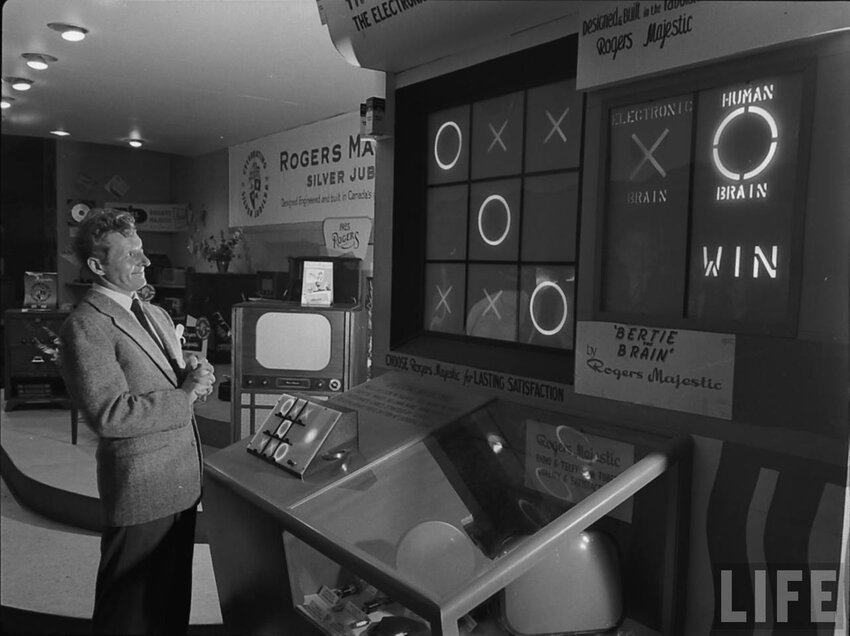
\includegraphics[width=4.23035in,height=3.16667in]{MyThesisImages/media/image3.jpeg}	
\caption{Life magazine photo of comedian Danny Kaye standing in front
of Bertie the Brain at the Canadian National Exhibition in 1950 Source:\cite{QuantumGames}}
\end{figure}

Since then, artificial intelligence has been closely intertwined with
game development and can be separated in two distinct categories
Behavioral and Generative, used as a means of creating engaging enemies,
as well as never ending procedurally generated worlds.


\section{(Sub-chapter 2.1) Behavioral AI}

There are many ways to implement behavior inside a video game and
depending on the developers approach the results may greatly vary.
Mainly used in the creation of autonomous Non-Player Characters (NPC)
for the purpose of creating a more realistic environment and a
"living" world filled with enemies and friendly characters for the
player to interact with.

Many techniques from the academic field are utilized in creating
believable characters and varied behaviors in video games but sometimes
complex and costly in terms of computational power are most of the time
avoided, because the developers desire a degree of control in certain
interactions.


\subsection{(Section 2.1.a) Finite State Machines}

The first and simplest form of creating a behavioral AI inside a game is
using a finite state machine (FSM) in order to simulate the behavior of
an NPC. \cite{syahputra_2019_historical,jagdale_2021_finite,tengkusyahdinariyan_2023_implementation,sweetser_2002_current,utesch_2017_the,fathoni_2020_finite,aversa_2018_unity}

\begin{figure}[H]
	\centering
    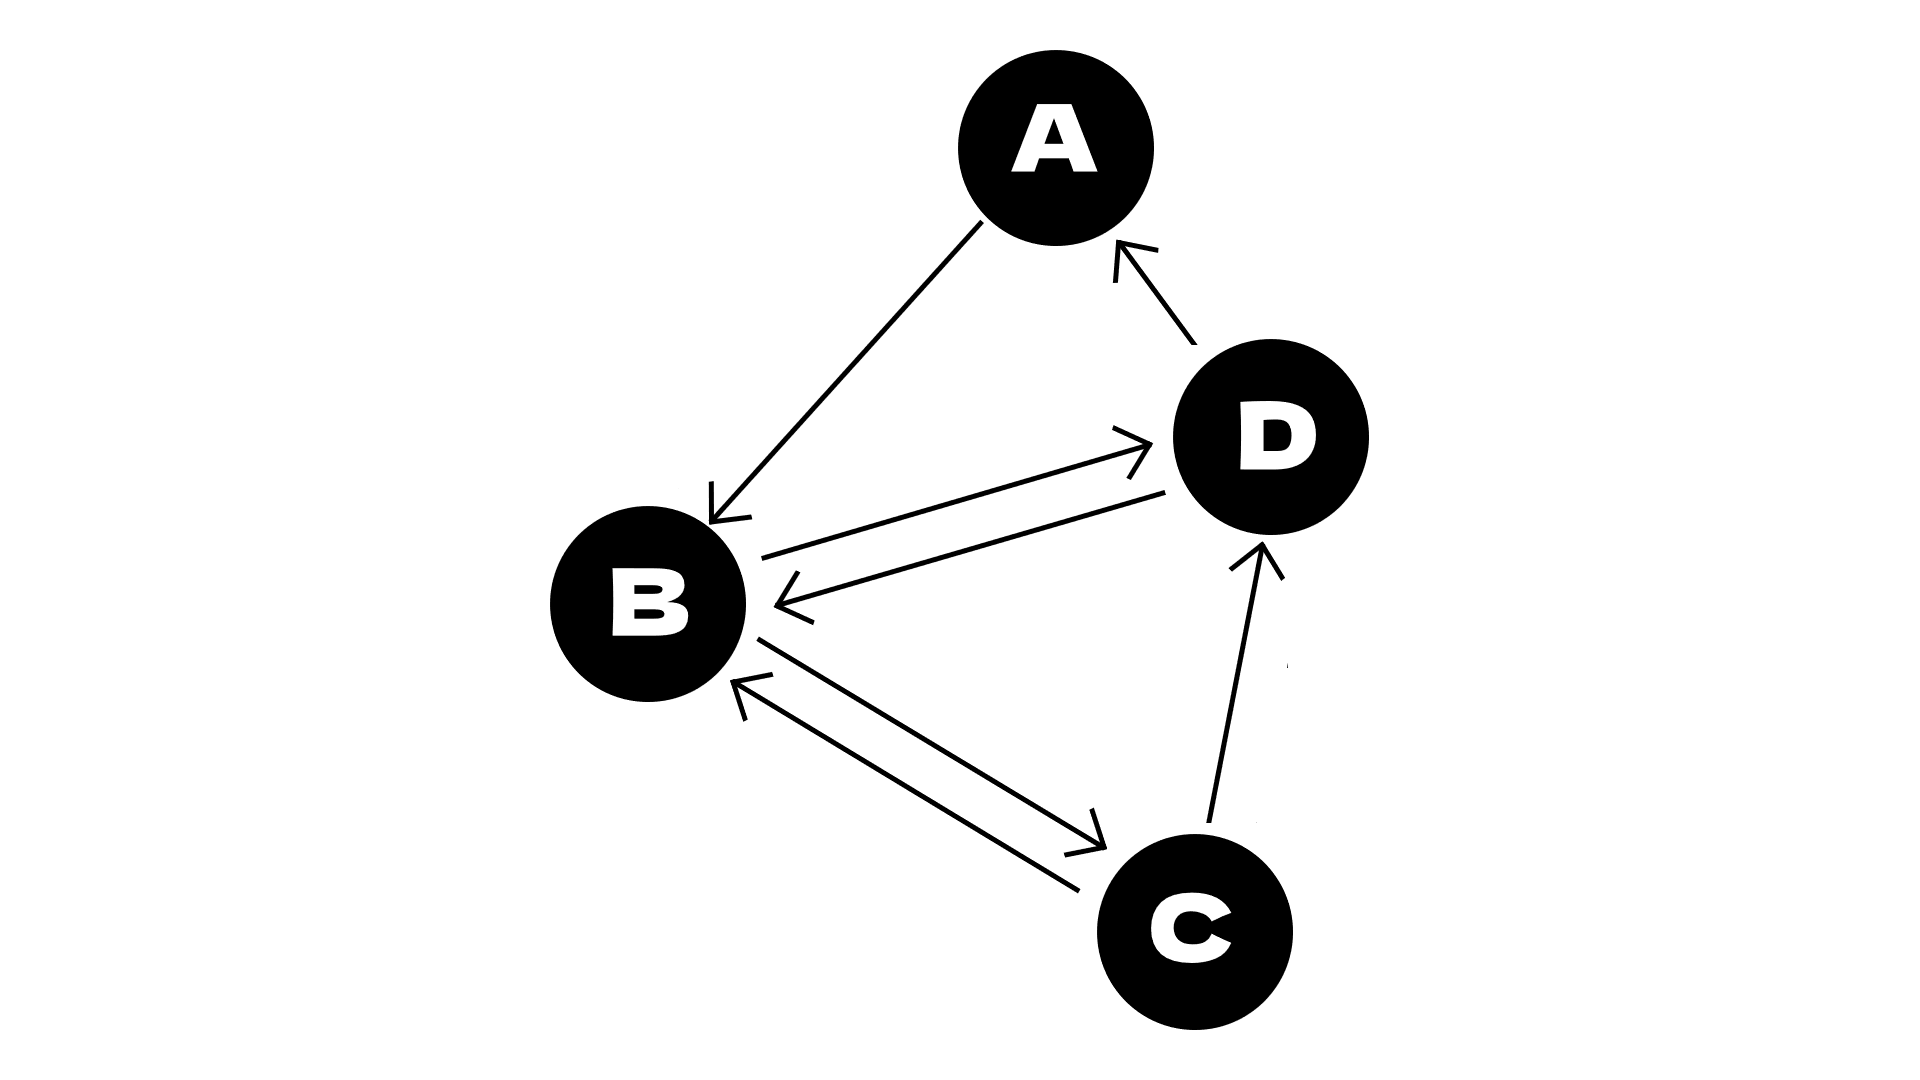
\includegraphics[width=4.31478in,height=2.425in]{MyThesisImages/media/image4.png}
	\caption{Example of Finite State Machine Behavior Control}
\end{figure}

This example FSM represents a simple enemy NPC behavior. Each circle
represents a state of the FSM, A: patrol, B: Hunt, C: Attack, D: Seek.
The enemy keeps track of many in game variables and transitions between
states on the FSM depending on those.

Consider the scenario of an enemy being in state A: patrol, after player
character is in sight transition to state B: Hunt, if player is within
attach range transition to state C: attack. If the player runs away,
then transition back to state B: Hunt. If the player leaves line of
sight transition to state D: Seek. If certain window of time passes and
the player is not found, then transition to state A: patrol. By
following the flow of a predefined FSM, a game can simulate the behavior
of an enemy character with ease.

Various propositions are made from the scientific community to combine
the concept of FSMs with multiple different technologies like fuzzy
logic \cite{andrea_2018_combination}, A* algorithm \cite{adegun_2020_design}, evolutionary programming
\cite{miranda_2015_improving,mora_2014_creating} and more in order to create better models for decision
making, path finding and NPC emotion status.

The complexity of FSMs increases rapidly based on the number of states,
they start to become more and more difficult to design. A Hierarchical
Finite State Machine (HFSM) \cite{hu_2011_componentbased} was the next step to combat the
shortcomings of traditional FSMs. HFSM is nothing more than an extension
of the basic FSM by creating composite states containing inside them
states and transitions, thus making a hierarchy of FSMs.


\begin{figure}[H]
	\centering
    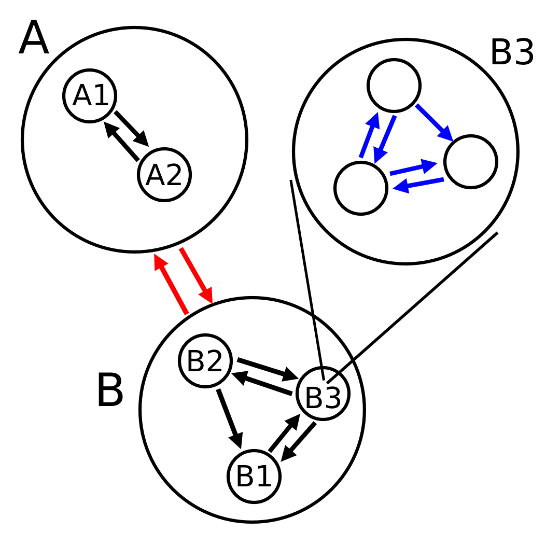
\includegraphics[width=2.54861in,height=2.54861in]{MyThesisImages/media/image5.png}  	\caption{Hierarchical FSM example. Same colored arrows represent interactions between states of the same level of hierarchy. B3 is zoomed out view of inner state of B.}
\end{figure}





\subsection{(Section 2.1.b) Behavior Trees}

Using Behavior Trees (BT) for game AI is the most common technique used
in current game development; they are a hierarchical structure of nodes
that control the flow of the decision-making process. Compared to FSM
approaches, BTs provide easier state transitions and are a simpler
method to create more complex behaviors. \cite{sekhavat_2017_behavior}

There are 3 types of nodes used in BTs, Composite, Decorator and Leaf
nodes.

\begin{enumerate}
\def\labelenumi{\arabic{enumi}.}
\item
  Composite nodes: can have one or more children of different types.

  \begin{enumerate}
  \def\labelenumii{\alph{enumii}.}
  \item
    Sequence: Behavior analogous to an AND logic gate. Executes all its
    children from first to last. If a child returns a failure the
    sequence stops and returns fail to the parent node. If the last
    child succeeds, then the sequence returns success to the parent
    node.
  \item
    Selector: Behavior analogous to an OR logic gate. Executes all its
    children from first to last. If the first child fails then continues
    to the second and so on, but immediately breaks and returns success
    to the parent when a child succeeds. Returns fail only if all
    children fail.
  \item
    Random Selector/Sequence: Identical functionality as Selector and
    Sequence but the order of visiting the children is randomized.
  \item
    Parallel: executing all its children at the same time
  \end{enumerate}
\item
  Decorator nodes: has only one child and affect its behavior or result.

  \begin{enumerate}
  \def\labelenumii{\alph{enumii}.}
  \item
    Inverter: Inverts the result of the child node. Similar to NOT logic
    gate
  \item
    Succeeder: always returns success regardless of the child's outcome.
  \item
    Repeater: repeat the process of the child node every time child node
    returns a result or for a set number of iterations.
  \item
    Repeat until fail: repeats the process of the child node until it
    returns a fail.
  \end{enumerate}
\item
  Leaf nodes: Task nodes that implement the actual actions of the AI.
\end{enumerate}


\begin{figure}[H]
	\centering
    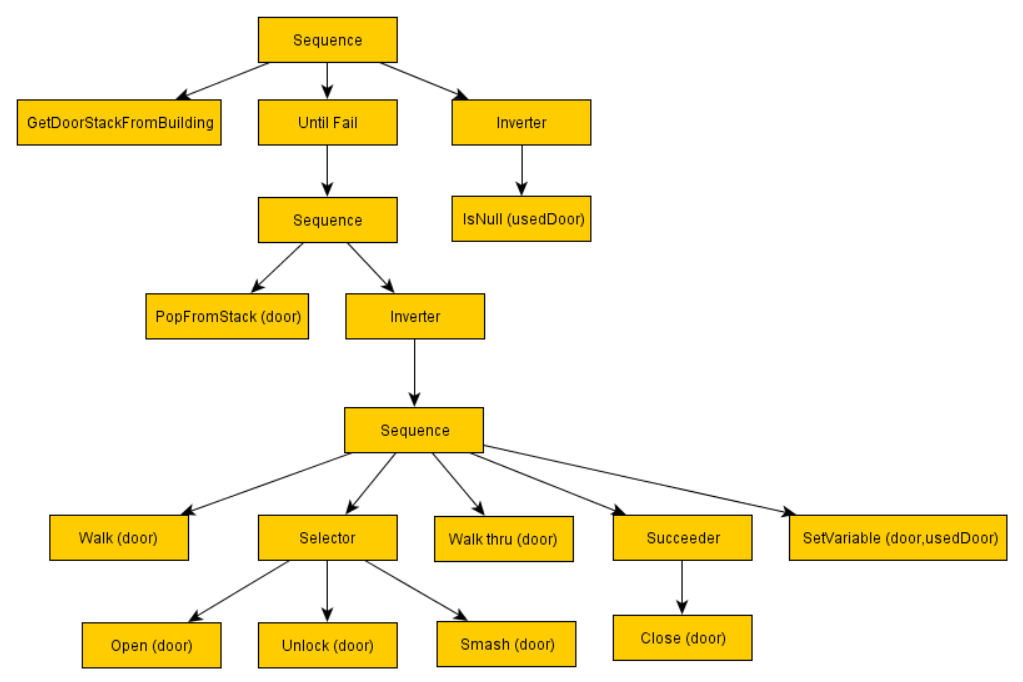
\includegraphics[width=4.56944in,height=3.04832in]{MyThesisImages/media/image6.png}	
    \caption{A behavior tree that will retrieve and then try to enter every single door into a building and return success if the character succeeded in getting in any of the doors, and it will return failure if they did not. Source:\cite{BehaviorTrees}}
\end{figure}

On top of this basic concept of a BT, many implementations have been
proposed by the scientific community as well as the development
industry. The main problem in creating BTs is in how to generate and
improve them in a manner that doesn't require much human intervention.

Using Genetic Algorithms to generate BTs has been explored in research\cite{zhang_2018_behavior}, Darwinian evolutionary methods can yield good results in
decision making, where genetic factors are used to generate improved
trees. The challenges of genetic algorithm implementations of BTs are
that they require a predefined initial population and the design of a
specific fitness function in order to evaluate the quality of generated
BTs comprising the population. Depending on the case this kind of
approach may not result in improved BTs.

A better method for generating and improving BTs is by observing expert
players and using their decision patterns as a means of constructing a
BT. Two such methodologies have been proposed, the first by Robertson
and Watson and the second by Tomai and Flores.

The Robertson-Watson\cite{robertson_2015_building} method creates a maximally specific BT
combining every action made by the players and then attempting to reduce
the tree by implementing a pattern recognition mechanism using the
Gapped Local Alignment of Motifs (GLAM2) software. Passing all sequences
to the GLAM2, which uses a simulated annealing approach to evaluate
matching patterns, and returning the new sequences and their scores when
they cannot be further improved after a set number of iterations. The
resulted sequences are evaluated by posing a threshold which discards
every sequence that scored below it and the remaining sequences are used
to construct the new BT.


\begin{figure}[H]
	\centering
    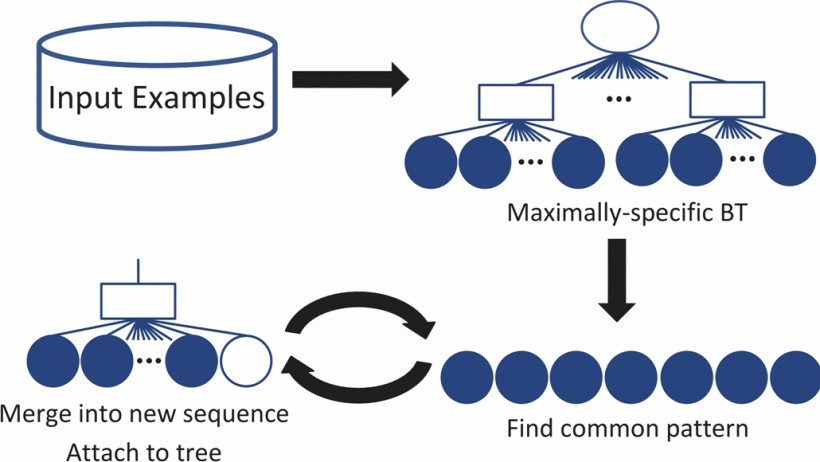
\includegraphics[width=2.89765in,height=1.63194in]{MyThesisImages/media/image7.jpg}	\caption{Overview of the Robertson-Watson approach. Source:\cite{robertson_2015_building}}
\end{figure}



\begin{figure}[H]
	\centering
    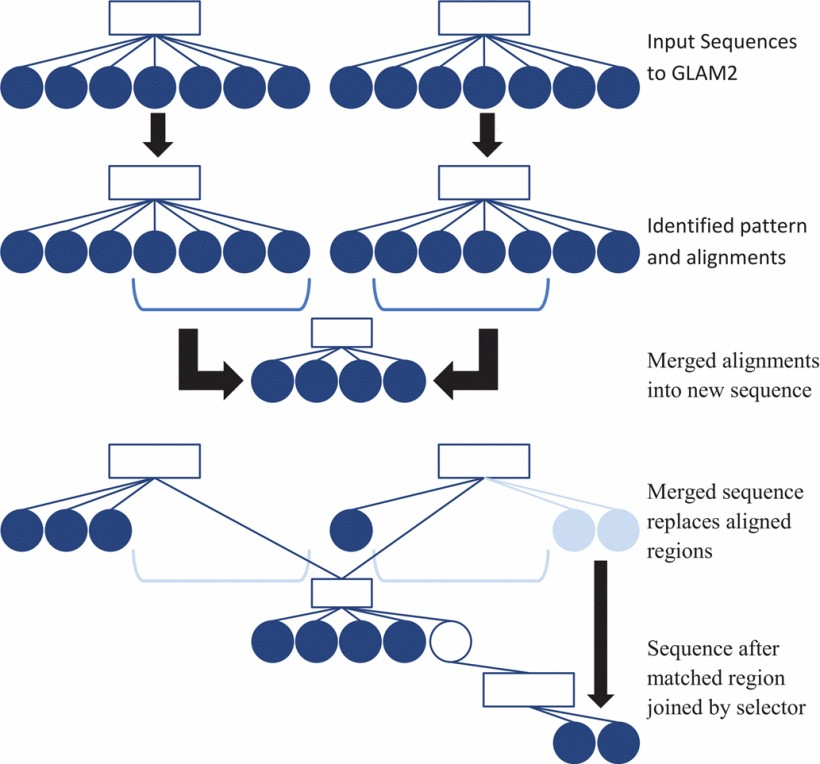
\includegraphics[width=2.72639in,height=2.54097in]{MyThesisImages/media/image8.jpg}	\caption{ Reducing the BT using GLAM2. Source:\cite{robertson_2015_building}}
\end{figure}


The Tomai-Flores\cite{tomai_2014_adapting} method proposes a Learning BT approach by
using a predefined BT, running an agent in sync with a playback
recording of a player and trying to match the actions of the player with
the behavior defined by the BT. If the player action diverges from the
expected, then the algorithm automatically tries to alter the structure
of the tree by adding Decorator nodes in order to create matching
human-like behavior. The most common example is the addition of delay as
players take time to consider their next action while the AI immediately
processes the next action in the BT. Another example of diverging player
behavior is when an enemy is killed the BT will automatically have the
agent loot the corpse, but in some circumstances, players may decide not
to loot and proceed to the next action.

The Tomai-Flores approach tries to closely imitate player actions in
order to create agents with human-like behavior. That has the
presupposes that the players always take objective oriented logical
actions, but in fact that is also not true, as many players run around
and jump aimlessly or make frantic movements while playing the game,
making the evaluation of the resulted agent behavior very challenging as
it is difficult to define what constitutes human-like behavior inside a
game environment.

Instead of observing players' actions, another proposal to improve
predesigned BTs is by implementation of utility theory approaches, to
attempt recreating believable game AI. This method does not alter the
structure of the BT but instead adds principles of calculating utility
for the purpose of selecting actions that will maximize the profit for
the agent.

A group of Chinese researchers\cite{fu_2016_Reinforcement}, proposed a reinforcement
learning method for adding utility in BTs. Traditional Selector nodes
have a left to right priority in child processing, they argue that a
more natural consideration would be to attach weight to each child and
by utilizing a reinforcement learning method of calculating those
weights it would result in a more believable agent behavior. To achieve that they implemented the Q-Learning algorithm for selector node optimization. Q-Learning introduces a state-action evaluation function with calculates the profit of each action given the agent's state and chooses the one that will result in the highest reward in an attempt to mimic human player behavior.

Another utility-based approach is presented by Simonov- Zagarskikh-
Fedorov \cite{simonov_2019_applying}, they introduce an intention-action system that chooses an action based on the agents' intentions. In the design phase
developers create behavior groups and intentions, they attach a list of appropriate intentions to each behavior group depending on the
personality they desire the agents of that group to have. During
gameplay the agents get a list of available intentions and choose the
best one given by a proposed utility evaluation function which considers environmental observations and personal characteristics, after that they calculate the utility trade-off for each intention-action pair and select the best action.

This approach produces believable agent behavior for agents of different
behavior groups, but agents of the same group will have predictable
behavior. To address this, they introduce Behavior Characteristics (BC)
variables that influence the utility calculation process and diversify
each agent based on individual circumstances. An agent may receive
temporary BCs depending on factors such as game area, health state,
mental state or game state.

One of the most popular game engines on the market, Unreal Engine (UE)
implements an Event-Driven approach of BTs \cite{UE_documentation_behavior}, instead of checking
for potential changes in every game tick, UE system passively listens to
relevant events that can be used to trigger changes in the BT. To
achieve this, conditionals are removed from the leaf nodes functionality
and instead are implemented as Conditional Decorators used as gates to
block off entire sub-trees or as observers by listening to events
triggers and if the conditions are met then they allow execution of the
subtree. By doing this the computational cost of visiting the BT is
decreased and thus achieving better game performance.


\begin{figure}[H]
	\centering
    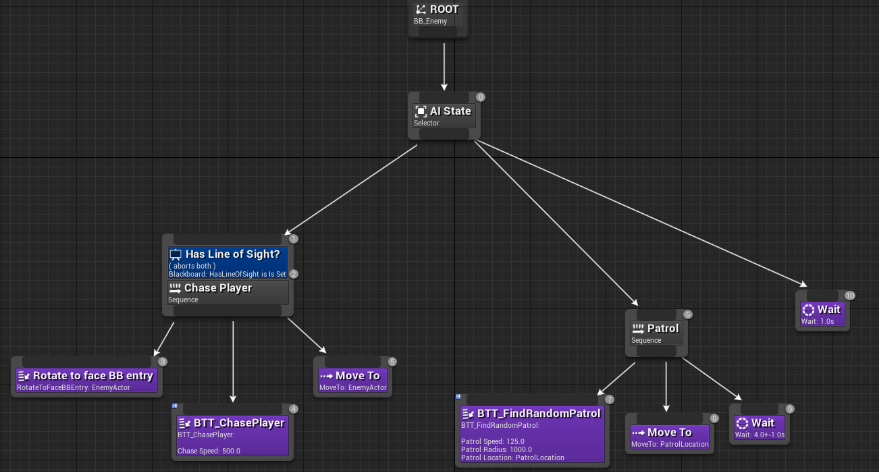
\includegraphics[width=3.97222in,height=2.2in]{MyThesisImages/media/image9.png}	
    \caption{Simple Unreal Engine 4 "Zombie" Behavior Tree. Source:\cite{UE_documentation_behavior}}
\end{figure}


\subsection{(Section 2.1.c) Neural Networks \& Deep
learning}

In order to simulate human brain function inside a digital environment
the scientific community developed the concept of Artificial Neural
Networks. These networks are represented as weighted directed graphs
consisting of "a layer of input neurons(nodes), one or
two or even three layers of hidden neurons and a final layer of output
neurons"\cite{wang_2003_artificial}. Video game environments are
ideal training grounds for neural networks as they provide a plethora of
use cases and training variables. Games can leverage this technology to
interpret input data and make probabilistic decisions to approximate
realistic responses in whatever scenario they are put through.

\begin{figure}[H]
	\centering
    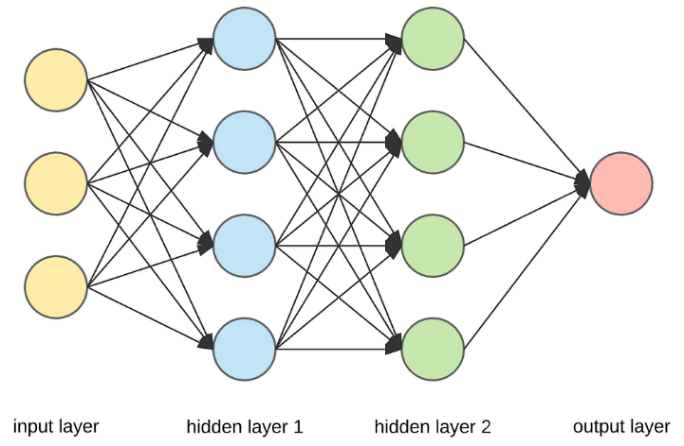
\includegraphics[width=2.99972in,height=1.96212in]{MyThesisImages/media/image10.png}
    \caption{Simple neural network graph representation. Source:\cite{dertat_2017}}
\end{figure}

Some of the most common uses of neural networks inside video games
include:

\begin{itemize}
\item
  \textbf{Environmental Scanning and classification}: The game AI can be
  taught to recognize audiovisual input from the environment and choose
  the appropriate response based on that.\cite{sweetser_2002_current}
\item
  \textbf{Memory:} The AI can learn a set of responses based on previews
  experiences and can choose how to respond to new situations. \cite{sweetser_2002_current}
\item
  \textbf{Prediction:} The network can be trained to recognize patterns
  in players' behavior, try to predict their next actions and respond
  according to this prediction.\cite{charles_2004_the}
\item
  \textbf{Behavior control:} The neural network can directly control
  the game AI by connecting the network's output as an input to various
  game engine variables. \cite{sweetser_2002_current}
\end{itemize}

\textbf{DEEP LEARNING}

"Deep learning is a subset of machine learning that uses multi-layered
neural networks, called deep neural networks, to simulate the complex
decision-making power of the human brain. By strict definition, a~deep
neural network, or DNN, is a neural network with three or more layers.
In practice, most DNNs have many more layers. DNNs are trained on large
amounts of data to identify and classify phenomena, recognize patterns
and relationships, evaluate possibilities, and make predictions and
decisions." \cite{ibm_2023_what}


\begin{figure}[H]
	\centering
    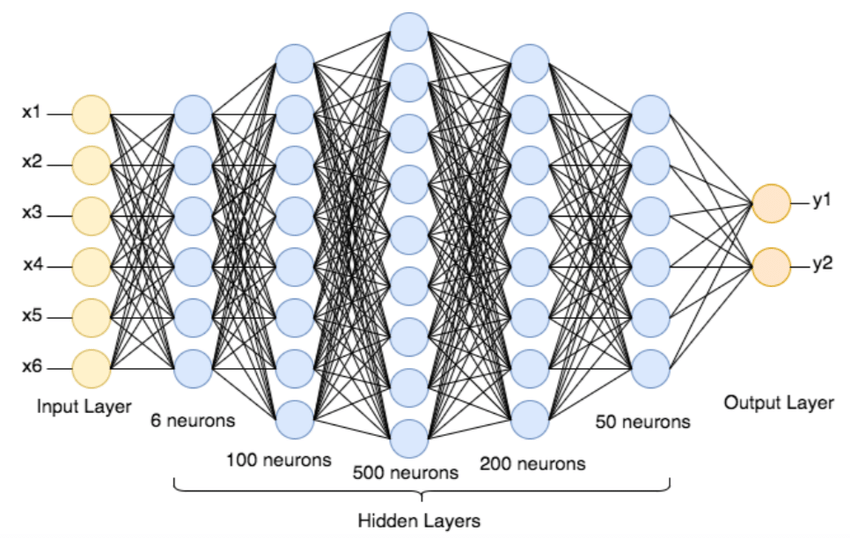
\includegraphics[width=3.96675in,height=2.51389in]{MyThesisImages/media/image11.png}
    \caption{Deep Neural Network Architecture Source:\cite{DeepNN}}
\end{figure}

By utilizing deep learning techniques to create the behavior of
autonomous agents, video games can make the next step in terms of
realistic behavior simulation.

The most popular deep learning approach in game development is deep
reinforcement learning, that combines the advantages of neural networks
and reinforcement learning technics to create agents who learn through
trial and error.

Model-Free Policy Gradient methods are commonly used as a means to solve
reinforcement learning problems such as the training of an agent inside
a video game environment and depending on the task at hand an on-policy
or an off-policy approach may be preferred.


\begin{table}[H]
    \centering
    \begin{tabular}{|m{17em}||m{17em}|}  
        \hline
        \centering
        On-Policy    & Off-Policy\\
        \hline
• Agent can pick actions. & • Agent cannot pick actions.\\
• Agent calculates state-action pairs to determine behavior policy. & •	Agent learns through explorations and plays without exploration.\\
• Agent always follows his own policy. & • Agent can learn from expert (imperfect human)\\
 &•	Agent can learn from sessions (recorded data)\\

    \hline
    \end{tabular}
    \caption{ Comparing On-policy and Off-policy}
\end{table}


According to Sutton and Barto (2018 2\textsuperscript{nd} edition)\cite{sutton_2020_reinforcement}, On-policy methods result in an agent that follows a safer
policy and as such don't take risky decisions, that makes the algorithm
converge faster but it is more likely to be trapped in local minima.

On the other hand, off-policy methods are greedy and agnostic, that
makes them less likely to get stuck in local minima thus increasing the
possibility to achieve optimal policy. Due to their greedy nature
off-policy technics result in an agent that takes more risky decisions
as it assumes that the agent will always take optimal future action.


\begin{figure}[H]
	\centering
    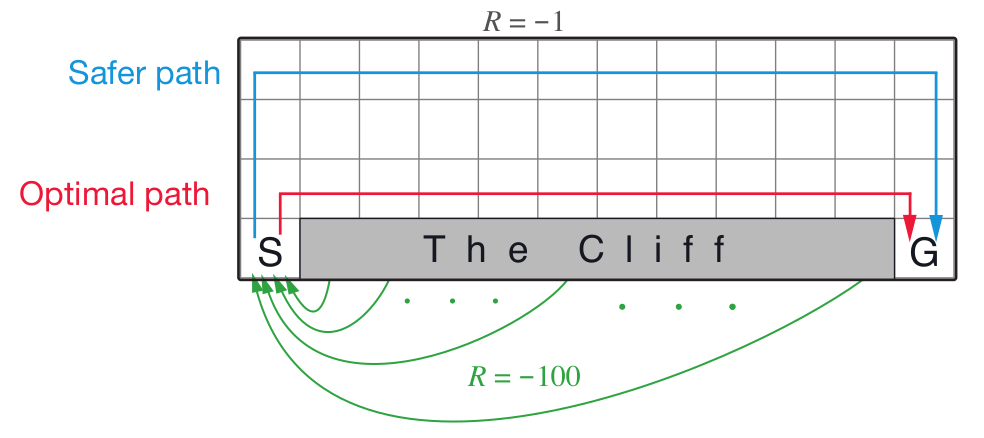
\includegraphics[width=4.38333in,height=1.95306in]{MyThesisImages/media/image12.png}\caption{Path finding comparison Blue is on-policy and Red is
    off-policy Source:\cite{sutton_2020_reinforcement}}
\end{figure}

\paragraph{Value-based and Policy-based\\}

Louis Owen in his article "Bird's-Eye View of Reinforcement Learning
Algorithms Taxonomy" \cite{owen_2020_birdseye} explains the distinction between
value/action based and Policy based approaches.

"The value-based methods try to pick the action which \emph{maximizes}
the action-state value function which will improve the policy in the
direction to the best policy (faster and lower variance), while
policy-based methods just take a little step and smoothly update in that
direction which is more stable but at the same time is less efficient
and sometimes leads to higher variance.


\begin{figure}[H]
	\centering
    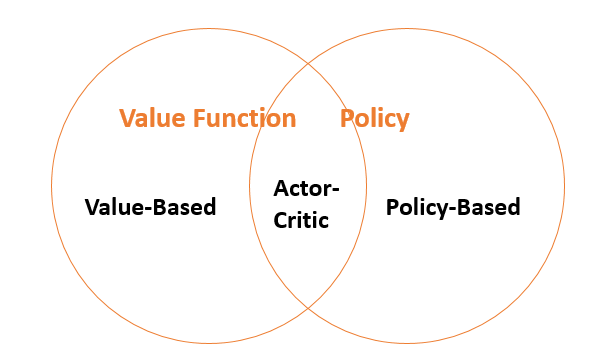
\includegraphics[width=3.66667in,height=2.17846in]{MyThesisImages/media/image13.png}\caption{Value-Based and Policy-Based Algorithms. {[}Image by Owen
Louis, Reproduced from David Silver's RL Course{]}}
\end{figure}

\begin{itemize}
\item
  \textbf{Value-based:} Agent aims to learn the value/action-value
  function in order to generate the optimal policy (i.e. the optimal
  policy is generated implicitly).
\item
  \textbf{Policy-based:} Agent aims to learn the policy directly using a
  parameterized function.
\item
  \textbf{Actor-Critic}: Agent aims to learn both the value function and
  the policy."
\end{itemize}

In implementations of video game AI value based and actor-critic
algorithms are commonly used, here we provide a list of popular
algorithms categorized appropriately.


\begin{table}[H]
    \centering
    \begin{tabular}{|m{10em}||m{10em}||m{10em}|}  
        \hline
        \centering
        & On-Policy    & Off-Policy\\
        \hline
        \centering
        
Value based & Deep SARSA	& Deep Q Network (DQN)\\
                            & & Double DQN\\
                            & &Dueling DQN\\
\hline
        \centering

Actor-Critic	&A3C&         DDPG\\
                &A2C&         TD3\\
                &TRPO&        SAC\\
                &PPO&	 \\
    \hline
    \end{tabular}
    \caption{List of common Deep Reinforcement learning Algorithms}
\end{table}

\textbf{Online and offline}

Charles and McGlinchey \cite{charles_2004_the} in their 2004 work on neural networks
denote that video game AI can fall in two categories online and offline
depending on whether the learning process stops or not after the release
of the final product.

The most common approach is to fully train the agent while the game is
in development and after the game's release no further improvements will
be possible on the agent's behavior. If that's the case, then the AI
falls in the offline category as its behavior has been developed only
prerelease by the game makers.

The second approach is to begin the agents learning process during the
game's development phase but continue to let the AI train itself after
the final release of the game by collecting data from players and
develop its behavior as an accumulation of different playstyles. This
method constitutes online learning as the AI continues to improve and
adapt its behavior by interacting with the end users.

\begin{figure}[H]
	\centering
    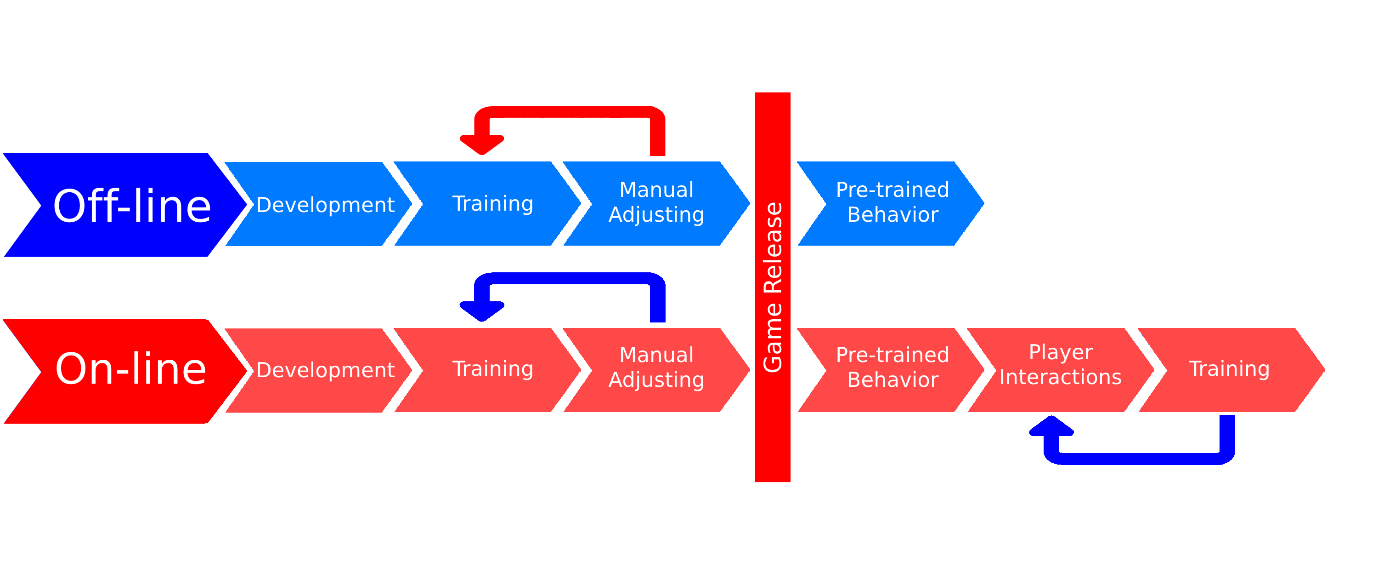
\includegraphics[width=6.04861in,height=1.83333in]{MyThesisImages/media/image14.png}
    \caption{Online and offline learning processes comparison.}
\end{figure}

Both categories come with their respective advantages and disadvantages. 
The offline method may produce a realistic agent behavior and the developers 
can make changes to account for undesirable or buggy behavior
before the game is released publicly, but that comes with the drawback
that the agent has a set behavior making it predictable after some time
and thus the players will learn to exploit its play patterns eventually.

On the other hand the online method will not produce predictable
gameplay for the agent as it continuously learns and changes its
behavior depending on the players it encounters in the game, but as
Barnes and Hutchens point out in "Testing Undefined Behavior as a
Result of Learning" (2002) \cite{barnes_2002_testing} " The most significant issue with
on-line learning is that it may produce unpredictable results; sometimes
these effects serve to enhance but more often it leads to erratic game
behavior that reduces the quality of gameplay, and in worse scenarios
will introduce dynamic game bugs. Testing, debugging and balancing games
that incorporate learning is a challenging task."

With online learning, the agent selects actions in real time based on
interactions with the video game environment, it is free to train the
policy using on-policy or off-policy updates. Offline technics employ a
pre-collected dataset without real-time interactions; therefore, they
are closely connected with off-policy methods.

\textbf{OPENAI FIVE}

OpenAI is considered one of the leading figures in the research of
artificial intelligence. In 2018 developed a multi-agent deep
reinforcement learning model named "OpenAI Five" \cite{openai_five} for playing
Valve's DOTA2 game. Dota2 is a Multiplayer online battle arena (MOBA)
where two teams comprised of five players each compete to subjugate each
other's base, inside a predefined area (arena).

The model is a scaled-up adaptation of the Proximal Policy Optimization
algorithm (PPO) that also includes a Long Short-Term Memory (LSTM)
network for each individual agent. Each LSTM is constituted by a single
layer of 1024-units that extract data from Valve's BOT API.



\begin{figure}[H]
	\centering
    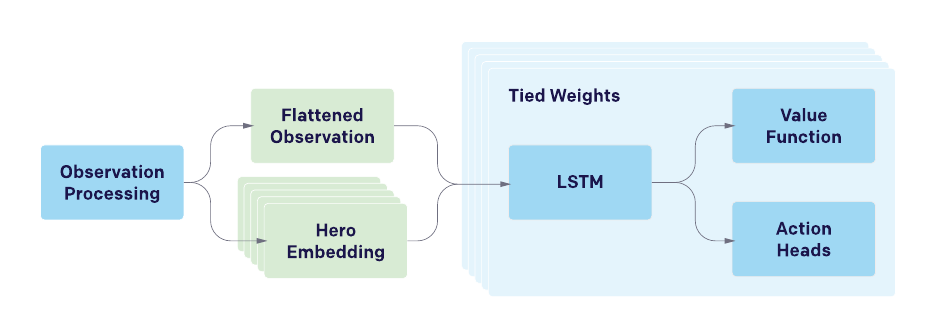
\includegraphics[width=6.25694in,height=1.83333in]{MyThesisImages/media/image15.png}
    \caption{Overview of the OpenAI Five model. Source:\cite{OpenAIFiveArch}}
\end{figure}

Open AI Five utilizes self-learning only and does not rely on data
gathered from human replays, the agent trains 80\% of its games against
itself and the other 20\% against its past selves. It starts from
randomized weights and tries to maximize the exponentially decayed sum
of future rewards, weighted by an exponential decay factor valuing
future rewards with a half-life of 46 seconds.

The metrics used to calculate the reward are the same that humans use to
calculate performance: net worth, kills, deaths, assists, last hits etc.

The AI heroes do not communicate with one another, the "team spirit"
hyperparameter is used to dictate how much each agent should care about
his individual reward versus the overall team's average reward.

Slowly but steadily the AI learned to play the game. In the beginning
the workers just wondered around aimlessly, after some training they
started to learn the concepts of laning, farming, fighting over mid and
steadily developed base level as well as high level strategies like
stealing bounty, champion rotations, five people push and more. OpenAI
Five averages around 150-170 actions per minute with a theoretical
maximum of 450 and has an average reaction time of 80ms, which is faster
than~humans. In live testing it managed to beat teams of amateur (93rd
percentile) and semi-professional (99th percentile) level.


\section{(Sub-chapter 2.2) Generative AI}

In the classical approach, video game content generation, also referred
commonly as procedurally generated content (PGC), is different than
modern generative AI. PGC focuses on generating adjustable game content,
"refers to all aspects of a game that affect the player experience but
are not non-player character (NPC) behavior or the game engine itself"\cite{yannakakis_2011_experiencedriven}
, such as textures, props, enemies, terrains, maps, levels,
quests, created by using a predefined set of assets as puzzle pieces to
mix and match together based on predefined algorithms.

A very popular approach on PGC proposed by Giannakakis and Togelius is
Experience Driven PGC \cite{yannakakis_2011_experiencedriven}, which leverages videogames as a prime ground for data mining from the player base in order to create models that generate content based on player preferences.

The main difference between PCG and Generative AI is that the first is
done at run time, resulting in a different experience for the player
each time he plays the game. Generative AI focuses on the development
phase of the game, as an assistive tool during the artistic process.

The objective of Generative AI is to create new synthetic data and
content from existing data sets by utilizing latent spaces which are
defined as abstract multi-dimensional spaces that encode a meaningful
internal representation of externally observed events. It works by
transforming raw data (image pixel values, soundwaves etc.) to suitable
internal representations inside a latent space. The distance between two
data points inside the latent space is dependent on the similarity of
the data before transformation. The more similar the raw data the closer
the distance of the latent representations. \cite{antoniadis_2022_latent}

The focus of this chapter will be on Latent Variable models, explaining
their inner workings and their practical uses as well as discussing some
of the scientific community's proposals and implementations of those
models that can be leveraged in game development applications.


\begin{figure}[H]
	\centering
    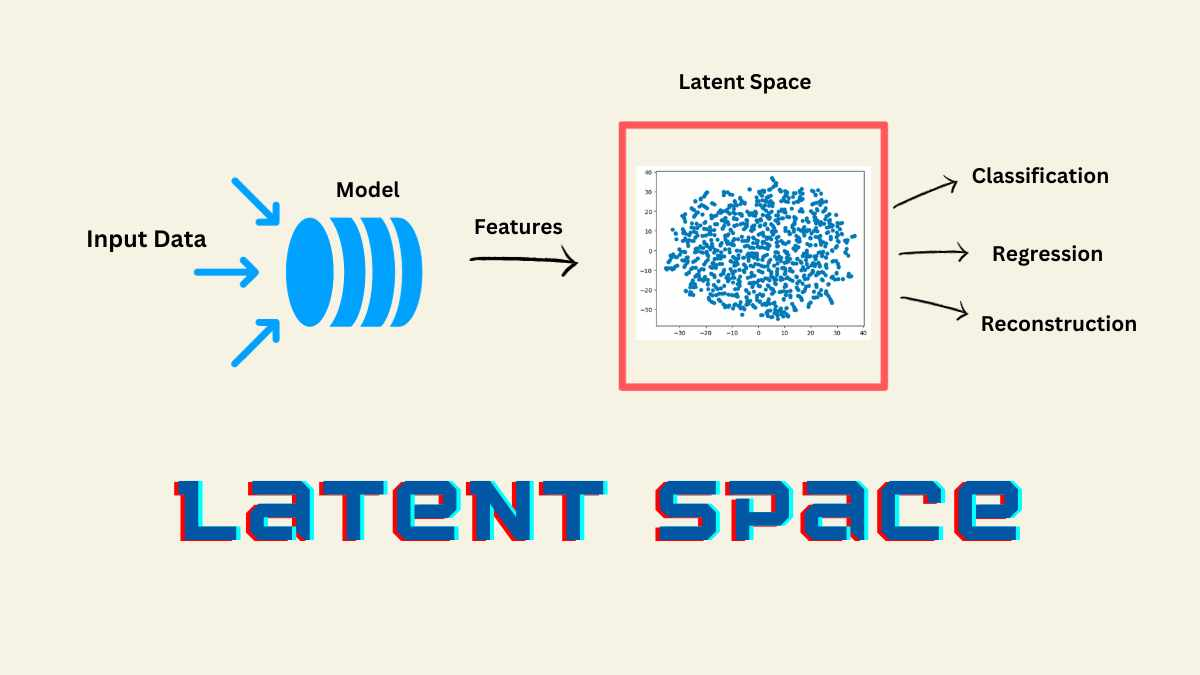
\includegraphics[width=5.8125in,height=1.97917in]{MyThesisImages/media/image16.jpeg}
    \caption{Simplified latent space representation. Source:\cite{verma_2023_Latent}}
\end{figure}


\subsection{(Section 2.2.a) Variational Auto-Encoders -- VAE}

Neural networks are a very useful tool in the machine learning world for
learning representations of complex data in a lower dimension domain.
The autoencoder architecture is based on two neural networks, the first
is the encoder and the second is the decoder. The "auto" part of the
name comes from the ability to automatically learn the best way to
encode the input data so that the decoder results will be as close as
possible to the initial input.

The encoder turns the input x to a latent representation z and the
decoders tries to decode z to x' while being penalized for how much
difference exists from x to x'.

Traditional autoencoder architecture results in sparsely populated
latent space which is desired in compression and denoising applications
but for generative purposes it is not optimal for predicting the
distribution of the values inside z.

Variational Auto-Encoders (VAE) have been developed to tackle that
sparsity problem, instead of feeding the latent variables to the decoder
they try to force the data to become normally distributed and therefore
more predictable. By utilizing the Kullback--Leibler divergence during
training they attempt to make a distribution of the latent space, for
the decoder to sample from, by calculating the mean standard deviation
to match as close as possible to the standardized normal distribution.

This process makes the VAEs capable of exploring variations in a more
specific direction retaining the characteristics of the input data while
providing the much desirable variation. Furthermore, with the inclusion
of meta-data in terms of labels can produce an even more guided VAE
model.

\begin{figure}[H]
	\centering
    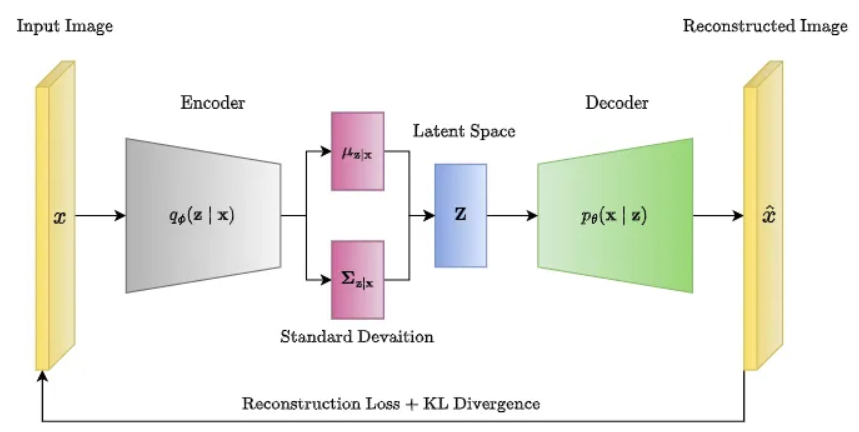
\includegraphics[width=4.6271in,height=2.32639in]{MyThesisImages/media/image17.png}
    \caption{VAE Architecture Source:\cite{shende_2023}}
\end{figure}

The main uses of VAEs include synthetic data generation, image
classification, image segmentation, image reconstruction and anomaly
detection, but most importantly they can be leveraged for their
excellent nonlinear latent feature representation learning capability.\cite{wei_2021_recent}

Hugo Wai Leung Mak and his colleagues Runze Han and Hoover H. F. Yin \cite{mak_2023_application}
did an extensive case study on applications of VAE model for
image processing in game design (2023). They experimented with level
generation from levels of the Arknights game, stylized anime girl avatar
generation and data clustering with the well-known MINST dataset.

\begin{figure}[H]
	\centering
    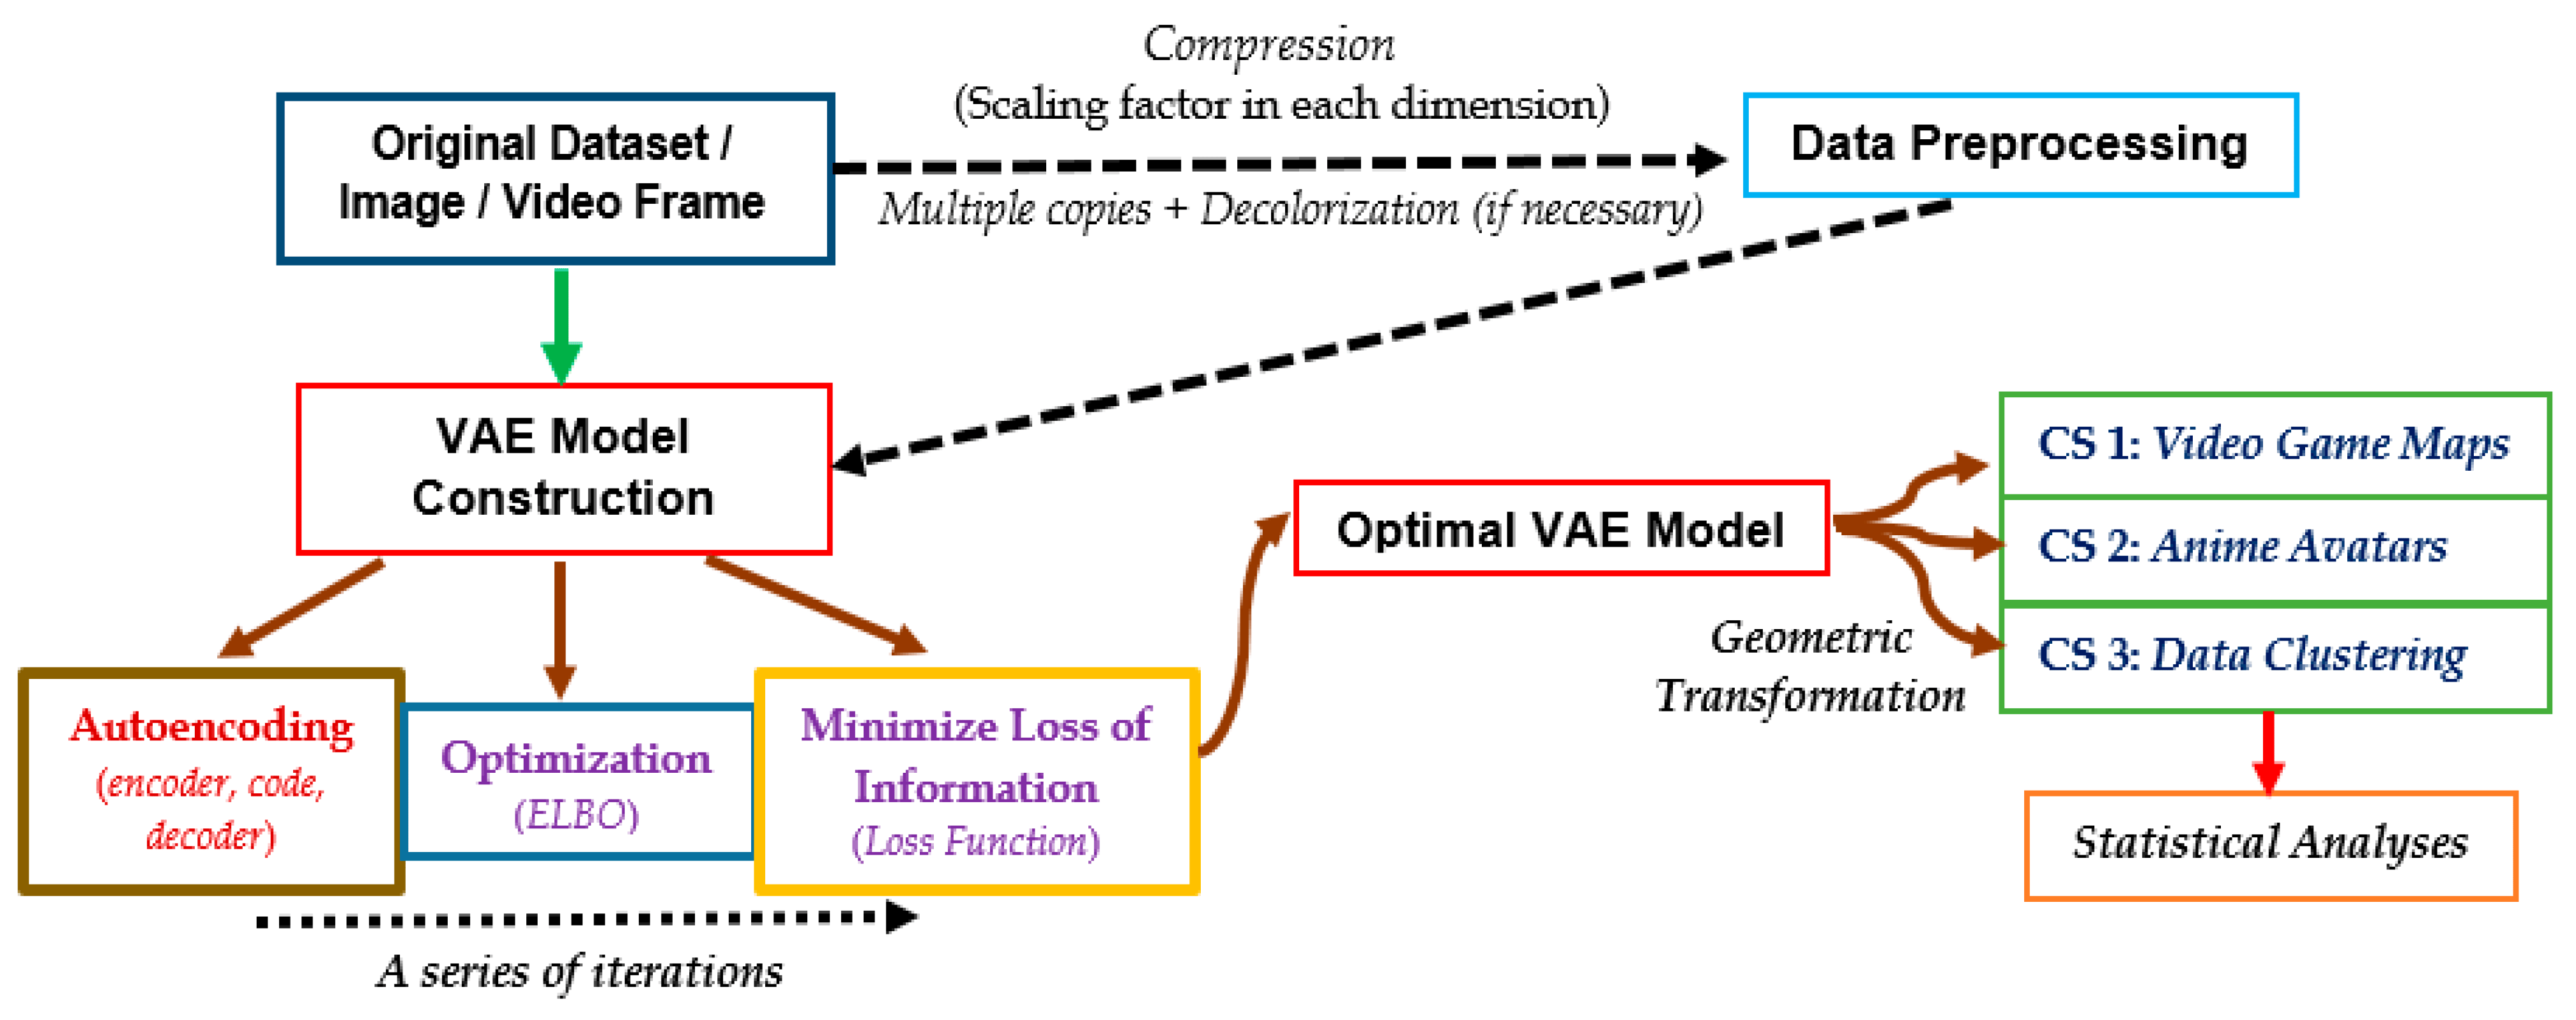
\includegraphics[width=6.25694in,height=2.47917in]{MyThesisImages/media/image18.png}
    \caption{Mak,Han,Yin VAE model. Source:\cite{mak_2023_application}}
\end{figure}


It was clearly illustrated in their research outcomes that VAEs are
capable of generating images in a specific pattern and show a lot of
promise in data clustering and in-game avatar generation, with the major drawback being the lack of resolution in the generated results.

They concluded that VAE models don't produce satisfactory results when
used as a standalone model, thus in order to overcome their shortcomings and make use of their strength, they should be combined with other
machine learning technologies such as Generative Adversarial
Networks-GANs and Long Sort Term Memory- LSTM with the goal to increase
the resolution of outputs, reduce training time and minimize the change
of "mode collapse".\cite{topal_2024_what}

\begin{figure}[H]
	\centering
    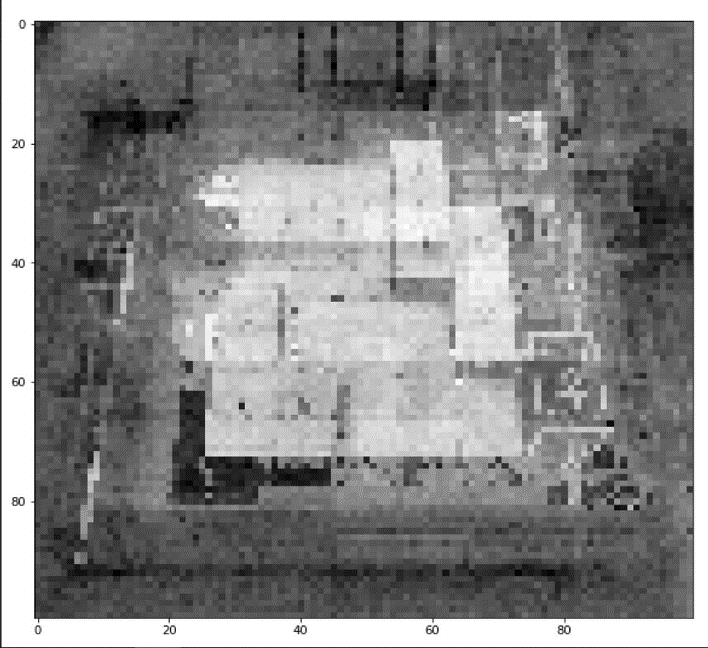
\includegraphics[width=3.18535in,height=2.91667in]{MyThesisImages/media/image19.png}
    \caption{The zoom-in version of an output game map of Arknights after the mixing of several processed images in the VAE model. Source:\cite{mak_2023_application}}
\end{figure}


\begin{figure}[H]
	\centering
    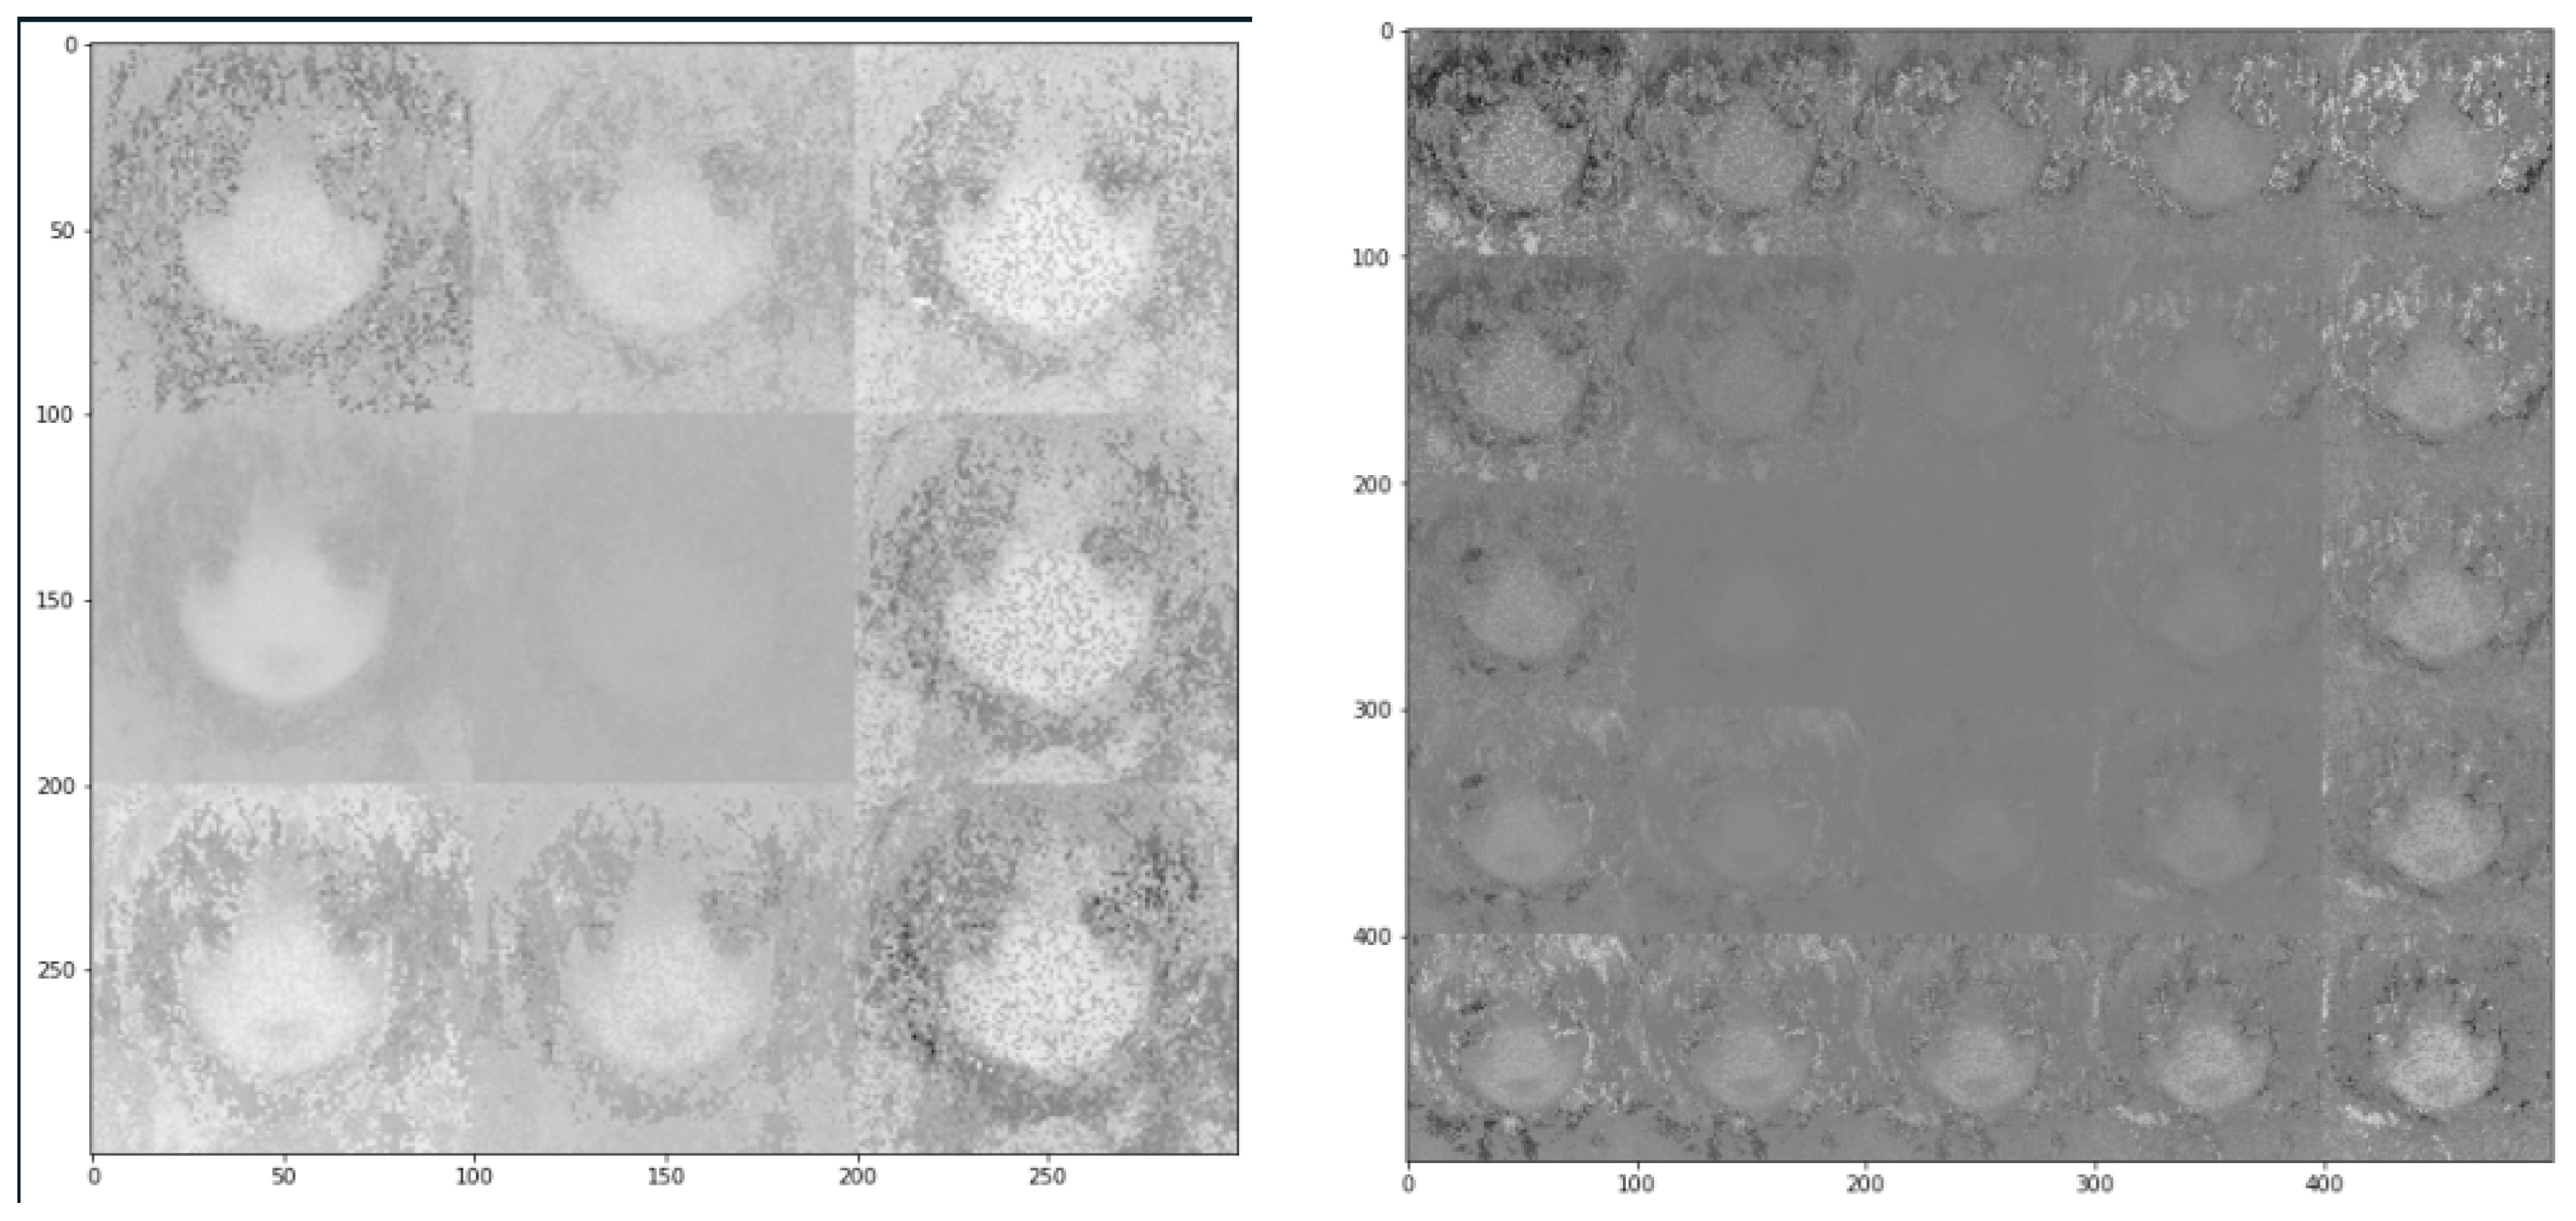
\includegraphics[width=4.22483in,height=2in]{MyThesisImages/media/image20.png}
    \caption{Two sample output images obtained from the VAE model based on the anime-girl dataset. Source:\cite{mak_2023_application}}
\end{figure}

Furthermore, the ability of VAEs to learn nonlinear latent feature
representations has made them an ideal sub-system of state-of-the-art
diffusion model frameworks, which will be discussed in a later section,
increasing their computational efficiency immensely as well as data
compression and reconstruction capabilities which are required due to
the large amount of data needed to train diffusion models.


\subsection{(Section 2.2.b) Generative Adversarial Network - GAN}

A GAN model consists of two neural networks which are trained at the
same time resulting at an adversarial competition. Jakub M. Tomczak\cite{tomczak_2022_deep}
in his book "Deep Generative Modelling" explains the concept
as a competition between a fraud and an expert. The fraud tries to
create a data in a specific style and the expert examines the data
created by the fraud in order to determine if they are real or fake. The
more they compete with each other the better they both will get but
given enough time the fraud will be able to create fake data that are
indistinguishable from the real data from the expert's perspective. We
name the fraud as generator and the expert as discriminator, we can
break the model as follows:

\begin{itemize}
\item
  A generator creates fake data from noise.
\item
  A discriminator that examines and classifies the generated data as
  real or fake.
\item
  Both the generator and the discriminator are parameterized using deep
  neural networks.
\item
  The networks are learned by using adversarial loss.
\end{itemize}

Most Common Types of GANs

\begin{enumerate}
\def\labelenumi{\arabic{enumi}.}
\item
  \begin{quote}
  \textbf{Conditional GAN-cGAN}: Introduced labels in order to generate
  data with specific attributes. Enables Text-to-Image generation. 
  Most popular implementations Pix2Pix, Pix2PixHD.\cite{melanie_2023_what}
  \end{quote}
  
  \begin{figure}[H]
	\centering
    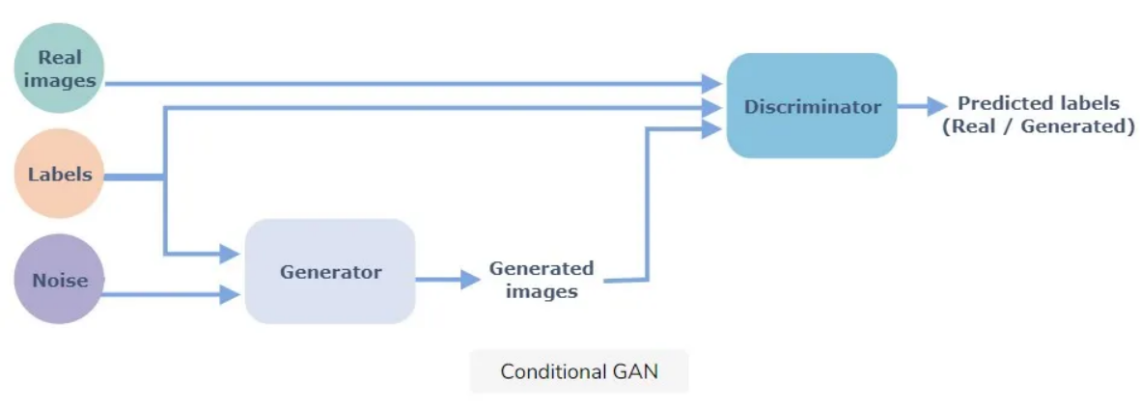
\includegraphics[width=5.15278in,height=1.84722in]{MyThesisImages/media/image21.png}
    \caption{ Overview of C-GAN architecture. Source:\cite{melanie_2023_what}}
\end{figure}

\end{enumerate}


\begin{enumerate}
\def\labelenumi{\arabic{enumi}.}
\setcounter{enumi}{1}
\item
  \begin{quote}
  \textbf{GAN with Encoders}: Uses encoder to learn the inverse mapping
  of the generated data back to the latent space.\cite{tsang_2021_review} Most popular
  implementations BiGAN, ALI.
  \end{quote}
\end{enumerate}

\begin{figure}[H]
	\centering
    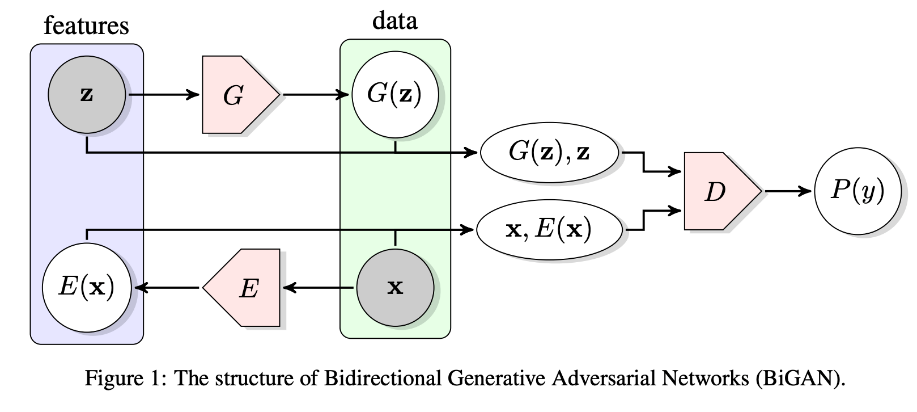
\includegraphics[width=4.15839in,height=1.61111in]{MyThesisImages/media/image22.png}
    \caption{BiGAN Architecture. In addition to the Generator G, an
encoder maps data to latent representations. The BiGAN discriminator
discriminate jointly in data space and latent space, where the latent
component is either an encoder output or a generator input. Source:\cite{BiGan_2017}}
\end{figure}


\begin{enumerate}
\def\labelenumi{\arabic{enumi}.}
\setcounter{enumi}{2}
\item
  \begin{quote}
  \textbf{StyleGAN}: Alters the generator architecture in order to
  generate photorealistic images of faces as well as images based on a
  specific style by using an intermediate latent space that contains
  style vectors.\cite{dhakal_2021_diving}
  \end{quote}
\end{enumerate}

\begin{figure}[H]
	\centering
    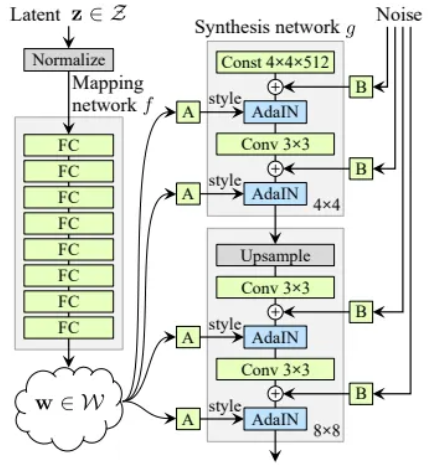
\includegraphics[width=2.38889in,height=2.55789in]{MyThesisImages/media/image23.png}
    \caption{StyleGAN Generator. Source:\cite{StyleGAN_2023}}
\end{figure}

\begin{figure}[H]
	\centering
    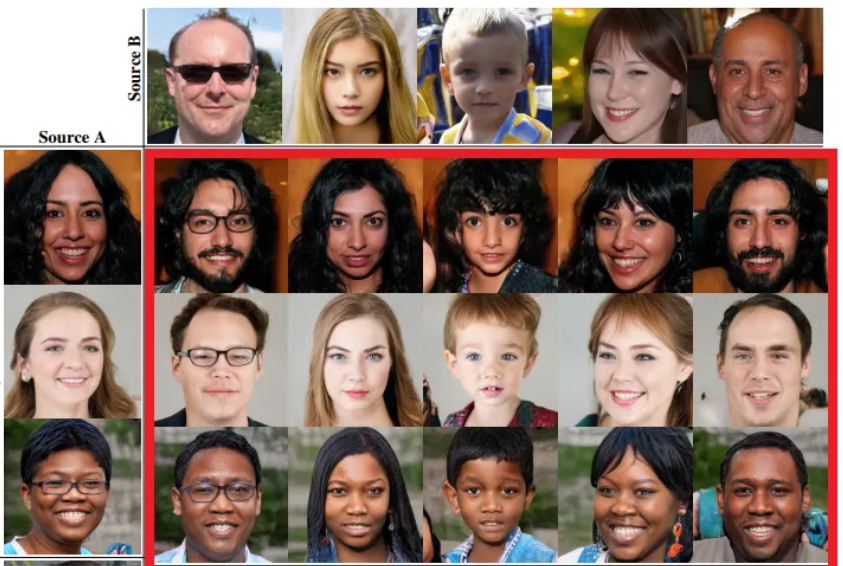
\includegraphics[width=3.91964in,height=2.63194in]{MyThesisImages/media/image24.png}
    \caption{StyleGAN Face mixing example. Source:\cite{StyleGAN_2023}}
\end{figure}

\begin{enumerate}
\def\labelenumi{\arabic{enumi}.}
\setcounter{enumi}{3}
\item
  \begin{quote}
  \textbf{CycleGAN:} Image-to-image translation without the need for
  one-to-one mapping from source to target. \cite{dhakal_2021_diving}
  
  \end{quote}
  
 \begin{figure}[H]
	\centering
    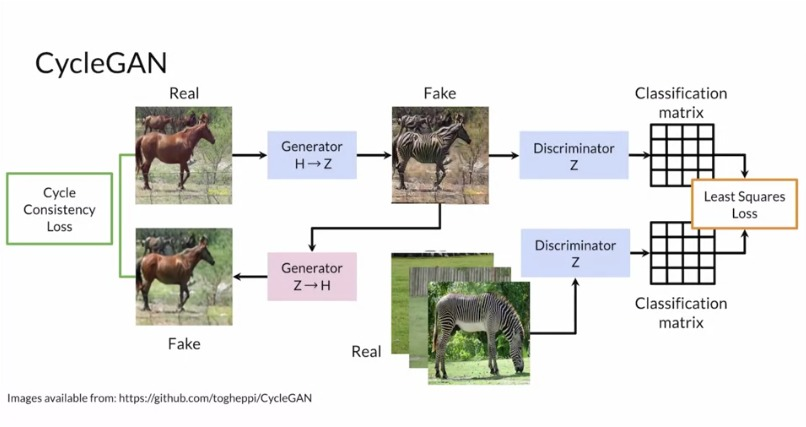
\includegraphics[width=4.80556in,height=2.54412in]{MyThesisImages/media/image25.jpeg}
    \caption{ CycleGAN architecture Horse to Zebra to Horse example.
    Source:\cite{CycleGAN_2020}}
 \end{figure} 
\end{enumerate}

\begin{enumerate}
\def\labelenumi{\arabic{enumi}.}
\setcounter{enumi}{4}
\item
  \begin{quote}
  \textbf{Deep Convolutional GAN-DCGAN}: Generally used for unsupervised
  learning. Replaced the MLP for a Convolution Neural Network.\cite{s_2021_generative}
  \end{quote}
  
\end{enumerate}

\begin{figure}[H]
	\centering
    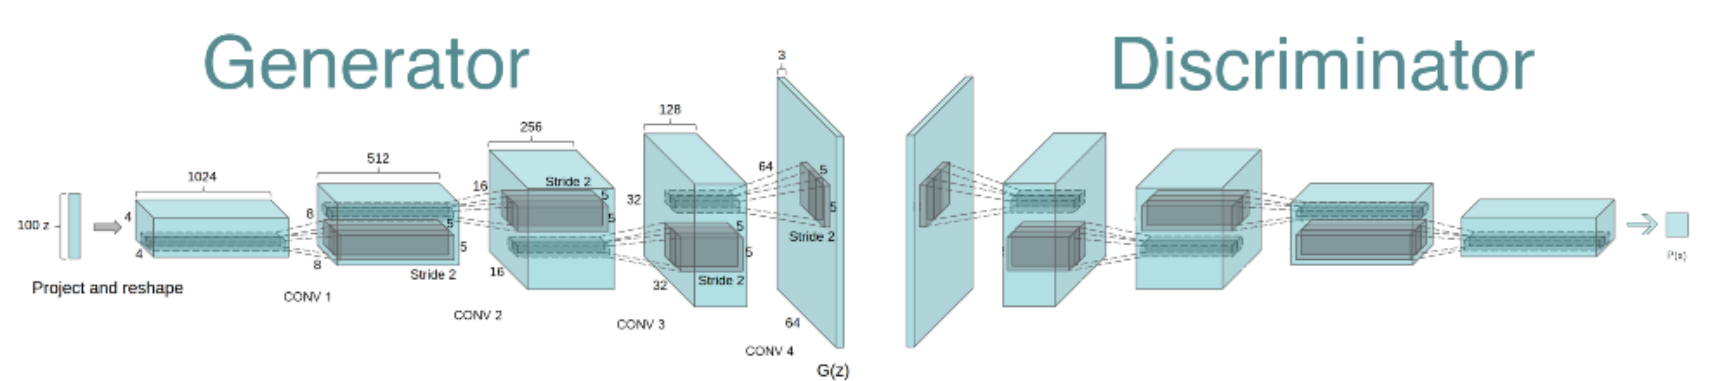
\includegraphics[width=6.26389in,height=1.39375in]{MyThesisImages/media/image26.png}
    \caption{ DCGAN architecture. Source:\cite{DCGAN_2022}}
\end{figure}


There are even more types of GANs that alter the metrics with which the adversarial loss is calculated such as Wasserstein GANs and f-GANs that use Wasserstein distance and f-divergence respectively.

The main limitation of the GAN model is called "mode collapse" that
happens "when the generator focuses on producing a limited set of data
patterns that deceive the discriminator. It becomes fixated on a few
dominant modes in the training data and fails to capture the full
diversity of the data distribution.

Just like the artist's fear of trying new styles, the generator avoids
exploring the entire data distribution in GANs. It produces repetitive
data samples, missing out on the rich variations present in the real
data." \cite{topal_2024_what}

Another problem that GANs suffer from is the inherent difficulty of
non-standardized evaluation metrics which depending on the application
may require the selection of a different metric in order to produce the desired results.

In respect of game development applications, GANs prove a very useful
tool for many areas, such as generating dynamic game environments,
seamless tileable textures, PBR material maps realistic terrains,
sprites, post-process effects, 3D models and super-resolution.

\paragraph{Dynamic Game Environments\\}

The problem of synthetic dynamic environment generation presented many
difficulties in the past years, and many proposed methods were riddled
with problems. "Action-LSTM models achieved success in scaling the
generated images to higher resolution but do not handle complex
stochasticity present in environments like Pacman. Recently proposed
VAE-based frameworks to capture the stochasticity of the task. However,
the resulting videos are blurry, and the generated frames tend to omit
certain details. GAN loss has been previously used in several works and
adversarial loss was used to disentangle pose from content across
different videos." \cite{kim_2020_learning}

In 2020 a team of researchers proposed a model called GameGAN \cite{kim_2020_learning}
by framing the problem as recurrent 2D image generation task to simplify
it. The general idea of the model is to train itself in an unsupervised
way by watching existing game footage, PACMAN and VIZDOOM were used as
examples. The model is capable of distinguishing between static and
dynamic game components as well as understanding the rules of the game
by observing the agent's actions during training.

A challenging problem in traditional image processing is the detection
of loop closures (returning to the same location), in this scenario the
GameGAN simulator must generate the virtual environment and maintain
temporal consistency during gameplay.

GameGAN is comprised of three components:

\begin{enumerate}

\item
  \begin{quote}
  \textbf{Dynamics Engine}: implemented as an action conditioned LSTM
  for the purpose of learning non-permitted agent actions like walking
  through walls and how other game components should behave in response to agent's actions.
  \end{quote}  
\item
  \begin{quote}
  \textbf{Memory module}: in cases where maintaining long-term temporal
  consistency is needed an external memory module is used to remember
  every scene generated.
  \end{quote}
\item
  \begin{quote}
  \textbf{Rendering engine}: a special implementation of standard
  transposed convolution layer-based renderer accounting for long-term
  consistency.\cite{anwar_2021_what}
  \end{quote}
\end{enumerate}


\begin{figure}[H]
	\centering
    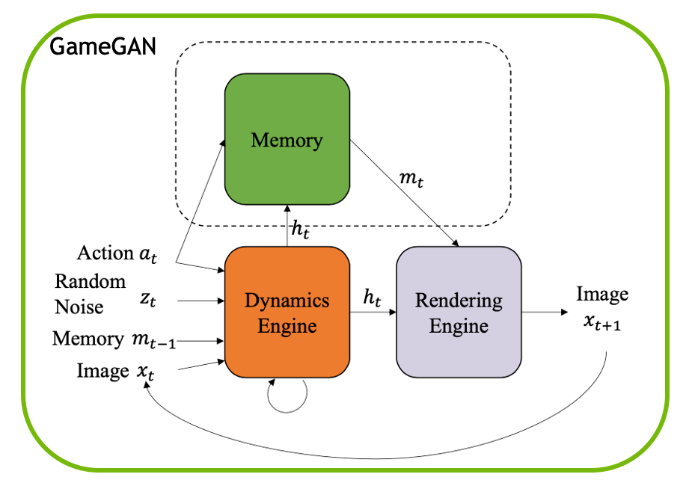
\includegraphics[width=3.12847in,height=2.20833in]{MyThesisImages/media/image27.png}
    \caption{GameGAN architecture. Source:\cite{nvidia_GameGAN}}
\end{figure}
 
As the model is capable of understanding the difference of static and
dynamic game components the researchers were able to create mix and
match games by combining static and dynamic components of two different
games at a time.

\begin{figure}[H]
	\centering
    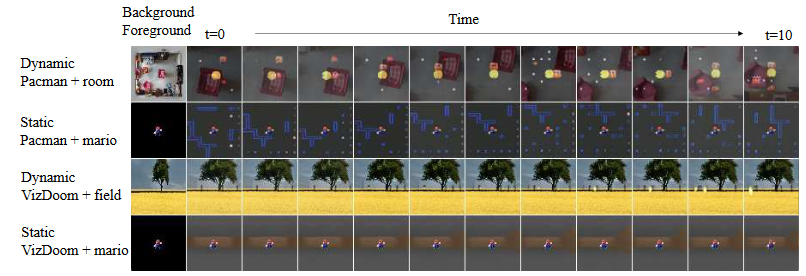
\includegraphics[width=6.25833in,height=2.14167in]{MyThesisImages/media/image28.png}
    \caption{GameGAN Element Swapping. Source:\cite{kim_2020_learning}}
\end{figure}


One year later (2021) Ghasemshirazi et al. \cite{ghasemshirazi_2021_mcgan} proposed a model
improving upon the work done in GameGAN, the new model was called
Multi-Class GameGAN (MC-GAN). MC-GAN adds upon the player agent
egocentric approach of the GameGAN and uses a MultiGAN Analyzer
framework in order to train an Inner Model for each individual enemy
type agent of the game, the player agent as well as every static element
of the game. They achieve that by training a new version of the game
with the camera focused on the desired component, for agents of the same
type; the camera perspective is changed and for static components the
camera is focused on them while the player agent seems to be fixed.

It is very obvious that the data complexity produced by the MultiGAN
Analyzer is very big, therefore a Data Unifier is used to combine the
data from all the classes and get them ready for rendering.

\begin{figure}[H]
	\centering
    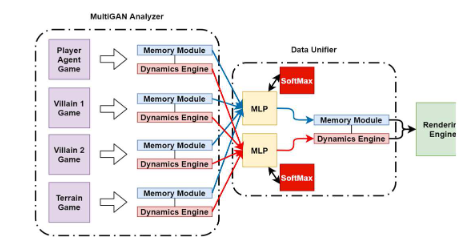
\includegraphics[width=4.71788in,height=2.44444in]{MyThesisImages/media/image29.png}
    \caption{MC-GAN Architecture. Source:\cite{ghasemshirazi_2021_mcgan}}
\end{figure}

With this MultiGAN approach the model can not only disentangle static
from dynamic components but can understand the different static and
dynamic components. This enables the model to be able to swap between
individual components from games, not all the static or dynamic sets.
Another advantage of the MC-GAN is the ability to create additional new levels without the need of retraining for each one like the original GameGAN required.

As advancements continue, these methods start pointing to a new
generation of AI-powered game engines, that may emerge in the near
future, capable of creating mashup-games from combinations of existing
ones only by observing them.

\paragraph{Seamless tileable textures\\}

The game development process move often than not requires textures to be
applied in large surfaces, when that's the case then the artists
responsible for creation of those textures need to take in account the
tileability component and transform the texture in such a way that when multiple copies of itself are placed side to side then no seam will be
visible on the touching side.

The manual method inside an image editing software involves cropping the
texture image, transforming the parts in specific orientation, and using
stamps to remove the seams. It is labor intensive, and the process has
to be replicated for every texture individually.

Considering the advances in image in painting technology utilizing
Context Encoders \cite{pathak_2016_context} to generate a missing part of an image based
on surrounding context, someone might experiment creating seamless
textures by using the classic manual method but replace the removal of
the seams from stamps to context aware fill using technology.


\begin{figure}[H]
	\centering
    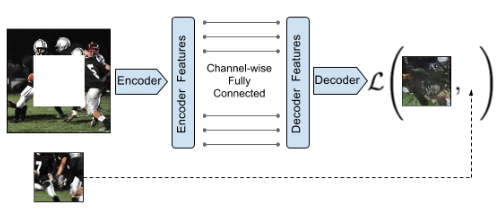
\includegraphics[width=4.15972in,height=1.73611in]{MyThesisImages/media/image30.png}
    \caption{Context Encoder Architecture with example. Source:\cite{pathak_2016_context}}
\end{figure}



Michael Cohen et al.\cite{cohen_2003_wang} proposed a Wang Tiles method of creating
seamless textures by sampling smaller parts of a bigger exemplar and
position samples with connecting borders next to each other. It has
shown great results, but a big problem remains, an initial texture is
required. Nowadays with the huge explosion in image synthesis technology
this doesn't pose such a difficulty.

\begin{figure}[H]
	\centering
    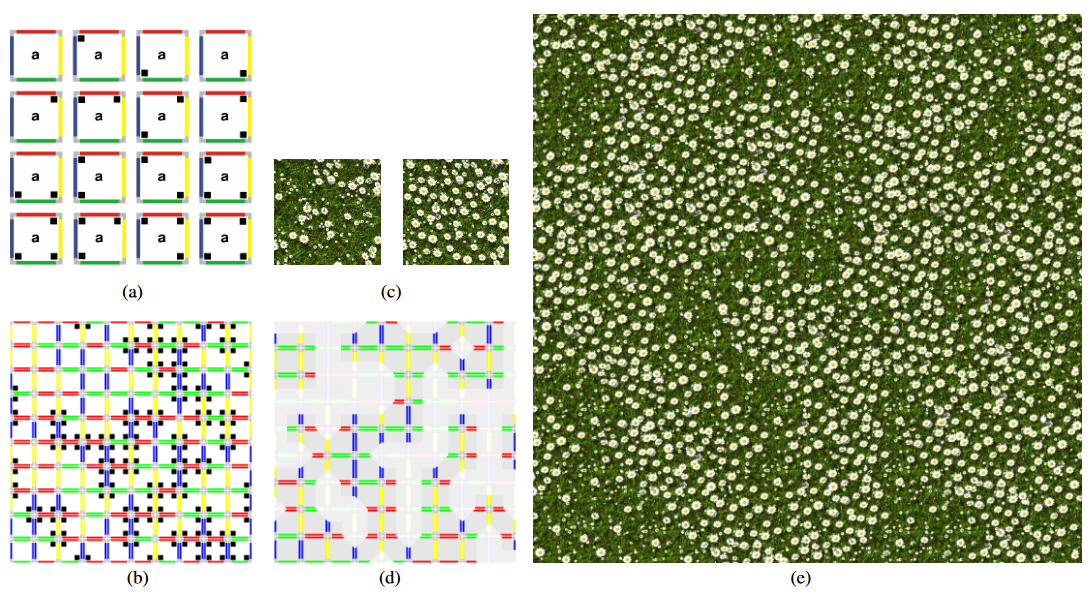
\includegraphics[width=6.04167in,height=3.31555in]{MyThesisImages/media/image31.png}
    \caption{a) A Wang tile with all combinations of marked corners. b)Tiling from the expanded tile set that shows various combinations of marked/unmarked tile corners. c) two source images d) tiling that contains density information. e) a tiled plane (12x12) constructed from a tile set with inhomogeneities. Source:\cite{cohen_2003_wang}}
\end{figure}


Another approach is to try generating a new seamless texture instead of
trying to make an existing one seamless. "Creating tileable textures is
a very challenging problem, as it requires a semantic understanding of
the repetitive elements, often at multiple scales."\cite{rodriguezpardo_2023_seamlessgan} A proposal
for a SeamlessGAN model was made by Rodriguez and Garces in 2023
\cite{rodriguezpardo_2023_seamlessgan}. The model is capable of generating an entire seamless texture
stack (different PBR maps) given an untileable input texture stack.

It works in two steps, in the first step uses crops of the input stack
to train a GAN that can generate new untileable textures double the
spatial resolution of the input , in the second step a latent space
concatenation is performed by repeating the latent space, created by the
GAN's generator, horizontally and vertically, after the new latent field
is passed through a decoder to remove discontinuities as well as
artifacts and after the decoding process we obtain four copies of the
original input crop with seamless transitions between them. The final
seamless texture is achieved by cropping the central area of the decoder
output textures put in 4x4 grid.

\begin{figure}[H]
	\centering
    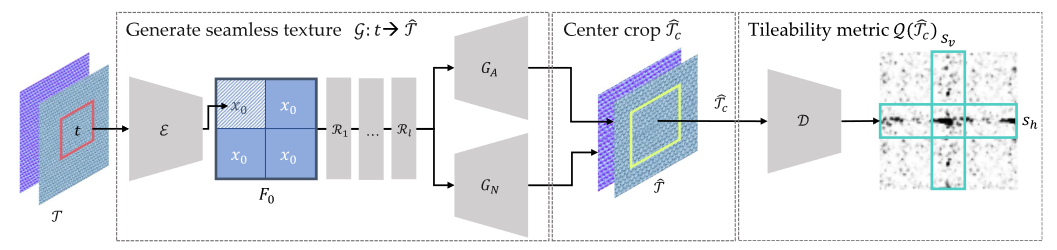
\includegraphics[width=6.26389in,height=1.47917in]{MyThesisImages/media/image32.png}

    \caption{SeamlessGAN Architecture. Source:\cite{rodriguezpardo_2023_seamlessgan}}
\end{figure}


The SeamlessGAN can generate different tileable textures depending on
the initial crop of the input texture and is currently the
state-of-the-art approach to seamless texture stack synthesis, with a
GAN, from single texture input and shown to outperform every other
competing implementation. A limitation of the model is that the
inter-map consistency, there is no guaranty that the different maps
(albedo, normal, roughness etc.) will have pixel-wise coherence as the
loss function is calculated separately for each one. Performing quality
evaluation on the generated textures reveals that the results are more
than satisfactory as the potential pixel inter-map inconsistencies are
most of the time not noticeable by the human eye.

\begin{figure}[H]
	\centering
    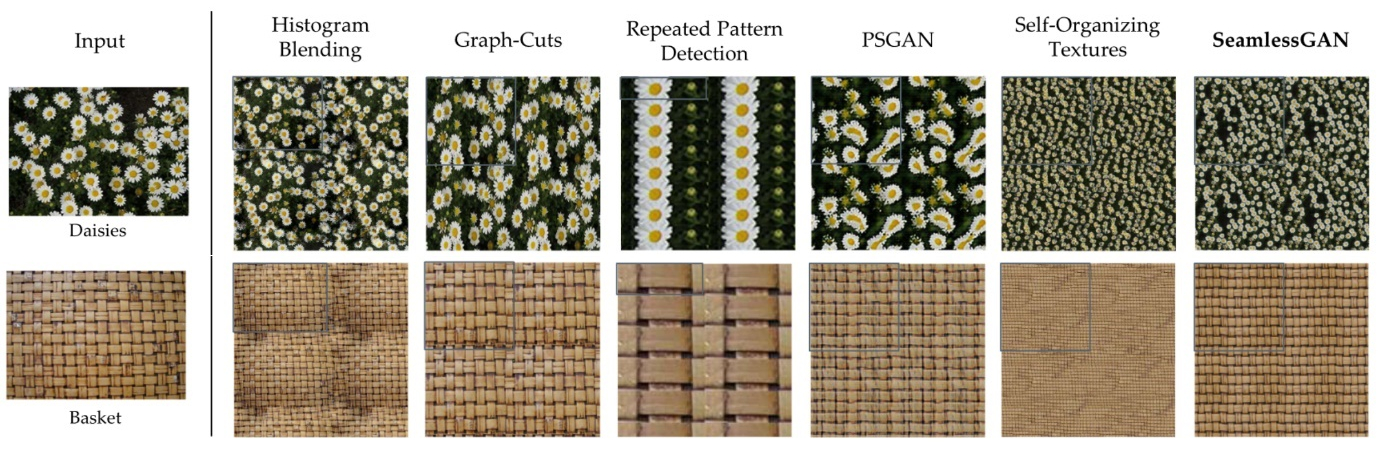
\includegraphics[width=6.25694in,height=2in]{MyThesisImages/media/image33.jpeg}

    \caption{Comparison of SeamlessGAN with other technics. SeamlessGAN method generally captures better the overall structure of the texture, while providing seamless and semantically coherent borders, for enhancing tileability. Source:\cite{rodriguezpardo_2023_seamlessgan}}
\end{figure}


\textbf{PBR material maps}

As discussed previously, generating pixel-perfect coherent texture
stacks is very difficult even if we account for inter-map generation
loss there is no guaranty that it can be eliminated completely. Tom
Moore implemented a model for predicting PBR maps by utilizing the
pix2pix Conditional GAN \cite{moore_pix2pix}. The pix2pix method is dedicated for
image translation and can achieve better results in converting an albedo
texture to the respective PBR maps.

The method uses a simple albedo texture also referred as diffuse, or
color map can be referenced and used to generate the different maps used
in the PBR materials. For every texture map a separate model must be
trained therefore, at least 4 models are needed to produce the basic
maps normal, roughness(smoothness), height, ambient occlusion (AO).

\begin{itemize}
\item
  Albedo2normal: translates the albedo to the corresponding normal map.
\item
  Albedo2smoothness: translates the albedo to the corresponding
  smoothness map.
\item
  Albedo2height: translates the albedo to the corresponding height map.
\item
  Height2AO: translates the height map to the corresponding ambient
  occlusion map.
\end{itemize}


\begin{table}[H]
\centering
    \begin{tabular}{|p{8em}|p{8em}|p{8em}|p{8em}|}  
        \hline
 Albedo & Normal & Roughness    & Height\\
        \hline
        \centering
\raisebox{-0.5cm}{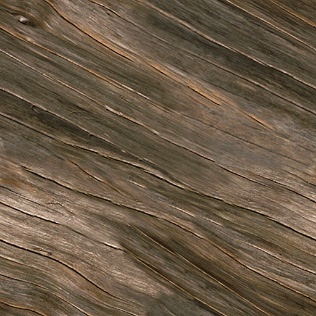
\includegraphics[width=3.5cm, height=3.5cm]{MyThesisImages/media/image34.jpeg}}&
\raisebox{-0.5cm}{
\includegraphics[width=3.5cm, height=3.5cm]{MyThesisImages/media/image35.jpeg}}&
\raisebox{-0.5cm}{
\includegraphics[width=3.5cm, height=3.5cm]{MyThesisImages/media/image36.png}}&
\raisebox{-0.5cm}{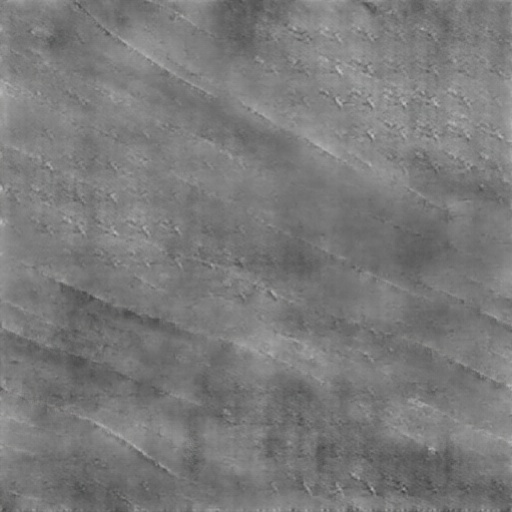
\includegraphics[width=3.5cm, height=3.5cm]{MyThesisImages/media/image37.png}}\\

\hline
Height	& AO & & \\
\hline
\raisebox{-0.5cm}{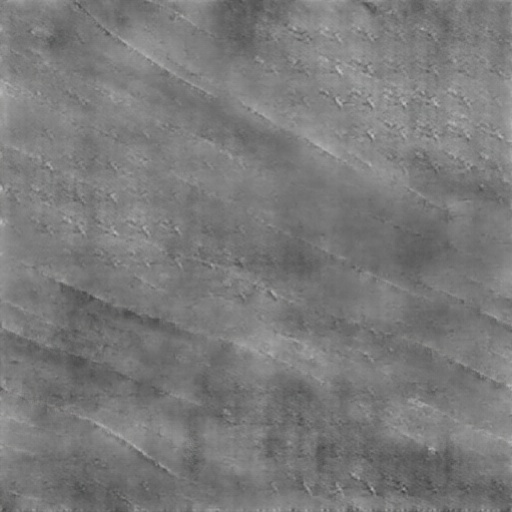
\includegraphics[width=3.5cm, height=3.5cm]{MyThesisImages/media/image37.png}}&
\raisebox{-0.5cm}{
\includegraphics[width=3.5cm, height=3.5cm]{MyThesisImages/media/image38.png}}& & \\
    \hline
    \end{tabular}
    \caption{Tom Moore's Pix2Pix model generated PBR maps. Source:\cite{moore_pix2pix}}
\end{table}

\paragraph{Post-process effects\\}

Post-process effects refer to rendering filters used in videogames in
order to enhance the visual experience of the player. Motion blur and
color correction are one of the essential uses of post processing
effects, but developers also use them to create alternative artistic
representations without the need to make changes to the game, it just
gets rendered differently.

Style transferring is a very prominent domain of GANs and there is a
plethora of methods proposed for image-to-image translation, but we will
focus on a videogame-based approach from Mittermueller, Ye and Hlavacs.\cite{mittermueller_2022_estgan}

These three researchers from the university of Viena proposed a method
to leverage the G-buffers used in game engines for rendering. "GBuffer
is short for Geometry Buffer, which means a buffer that stores geometry
information. More specifically, it refers to a group of render textures
used to describe object positions, normals, colors, and other
information needed for lighting." \cite{jiangwei_2023_a}

\begin{figure}[H]
	\centering
    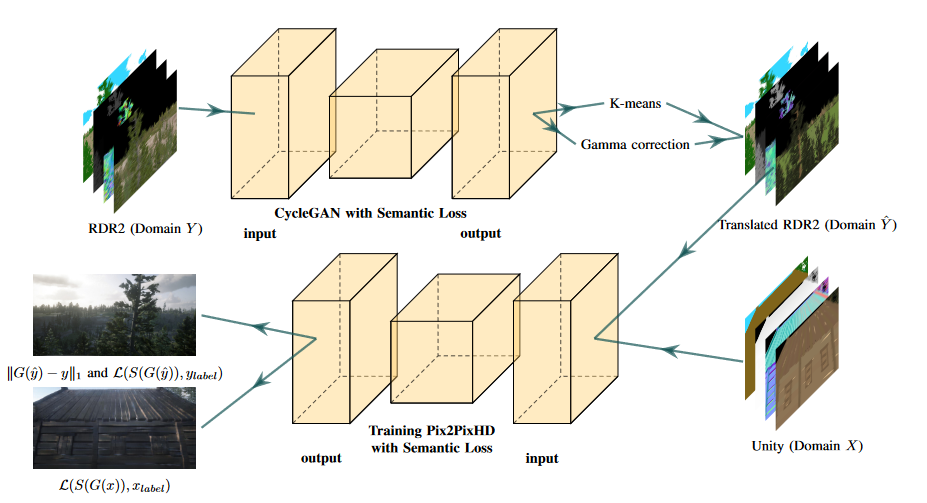
\includegraphics[width=4.18056in,height=2.33264in]{MyThesisImages/media/image39.png}
    \caption{Overview of EST-GAN Architecture. Source:\cite{mittermueller_2022_estgan}    }
\end{figure}

The model is called Enhanced Style Transfer GAN or EST-GAN for short.
EST-GAN uses a combination of a CycleGAN and a Pix2PixHD cGAN to produce
a game-to-game style transfer, Y is the game from which we want to
extract the style and X the game to which we want to apply the style
transfer.
\begin{figure}[H]
	\centering
    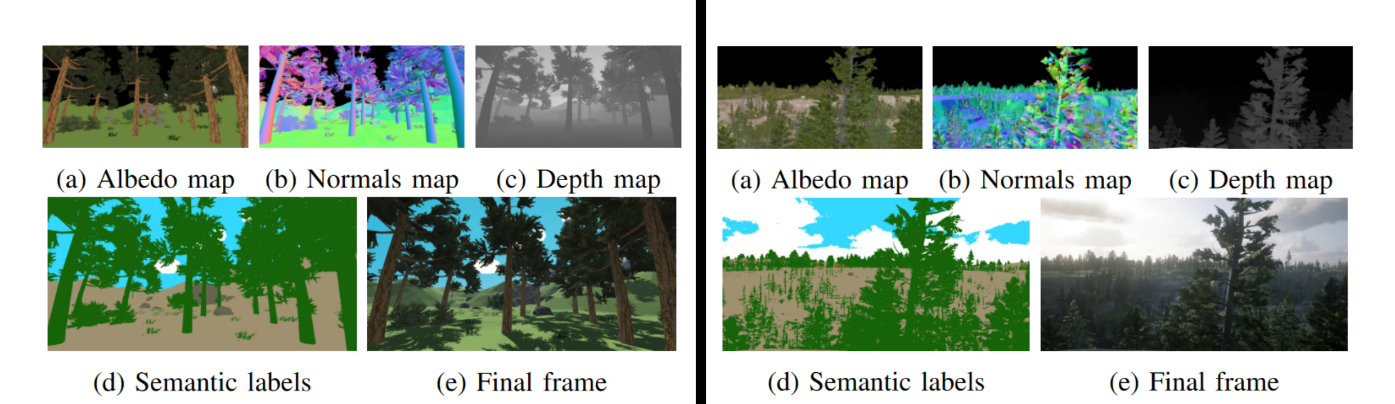
\includegraphics[width=6.00694in,height=2.65903in]{MyThesisImages/media/image40.png}
    \caption{Example of Sampled G-Buffer Frames.
    Left from Unity Domain X. Right from RDR2 Domain Y. Source:\cite{mittermueller_2022_estgan}    }
\end{figure}


The first step in the model used a CycleGAN to translate the G-Buffers
of the domain Y to the domain X but they observed that the default cycle
loss calculation method was producing undesirable results mainly
resulting in the model hallucinating vegetation where is should not be,
so a semantic loss method was used instead combined with mean absolute
error to result in matching probability distribution over all labels.
The new domain of translated G-buffers is called Ŷ.

\begin{figure}[H]
	\centering
    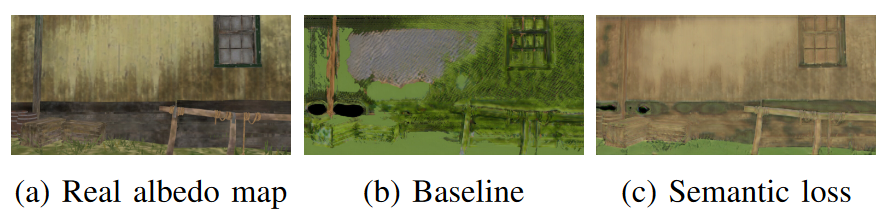
\includegraphics[width=4.59028in,height=1.1412in]{MyThesisImages/media/image41.png}
    \caption{ Comparison of a) Sampled Albedo b) CycleGAN generated Albedo c) CycleGAN+Semantic Loss Albedo. Source:\cite{mittermueller_2022_estgan}    }
\end{figure}


The second step is using the Pix2PixHD cGAN to create a translation
between the X and Ŷ. The inputs to the cGAN are the G-buffers from X as
well as the translated Y G-buffers. In this step semantic loss was used
as well as it was already implemented for the CycleGAN and produced very
impressive results with minor artifacts on normal maps in cases where
there were low polygon assets present

The third and last step was focused on removing artifacts produced by
the pix2pix cGAN in the normal maps as well as in the albedo maps from
the CycleGAN. The artifacts were a result of unsimilarity between the
sampled G-Buffers, due to low polygon objects in Domain X, compared to
Domain Y. A k-means clustering algorithm was used on the images to
remove those artifacts and produce sharp edges desired in the final
normal maps.


\begin{figure}[H]
	\centering
    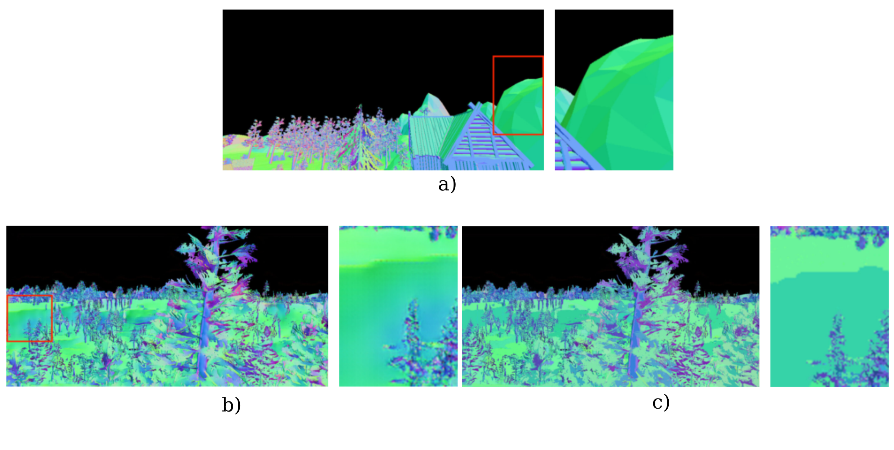
\includegraphics[width=4.04087in,height=1.85225in]{MyThesisImages/media/image42.png}
    \caption{ a) Domain X sharp normal edges b) Domain Y smoother edges c)Domain Y after Clustering. Source:\cite{mittermueller_2022_estgan}    }
\end{figure}

The researchers created a completely synthetic dataset with the use of
RenderDoc \cite{renderdoc}, which is a graphic debugger tool, used to capture
single frames as well as additional information like the G-Buffers. The
popular Red Dead Redemption game \cite{red_dead} was used for data collection
and as a target game the researchers created a simple nature scene
inside the Unity game engine to test the style transfer model.

\begin{figure}[H]
	\centering
    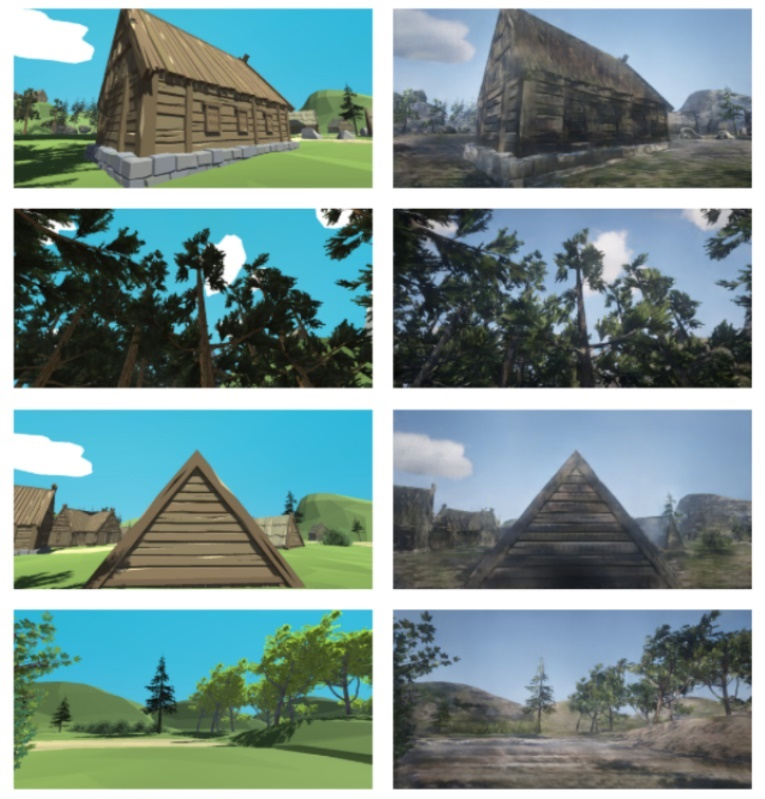
\includegraphics[width=3.47456in,height=3.63194in]{MyThesisImages/media/image43.jpeg}
    \caption{Left Baseline Unity Frame. Right EST-GAN final model produced Frame. Source:\cite{mittermueller_2022_estgan}}
\end{figure}

\paragraph{3D Models\\}

The generations of 3D models can be separated into two categories,
general 3D objects and 3D terrains which are a special case of 3D
geometry.

\begin{enumerate}
\def\labelenumi{\alph{enumi}.}
\item
  \textbf{General 3D objects}
\end{enumerate}

In literature 3D objects are represented in three different ways: point
clouds, meshes and voxel grids. Point clouds are sets of
multidimensional data points that contain space coordinated but can also
include additional information like color or velocity values. Meshes are
the most common representations of 3D geometry that are collections of
polygons that form the faces of the mesh in space. Each polygon consists
of edges, vertices, and an orientation vector. Voxel grids are 3D grids
organized in layers, rows, and columns. Voxel grids can be thought of as
fixed-size point clouds, where each voxel has a fixed size and discrete
coordinates.

\begin{figure}[H]
	\centering
    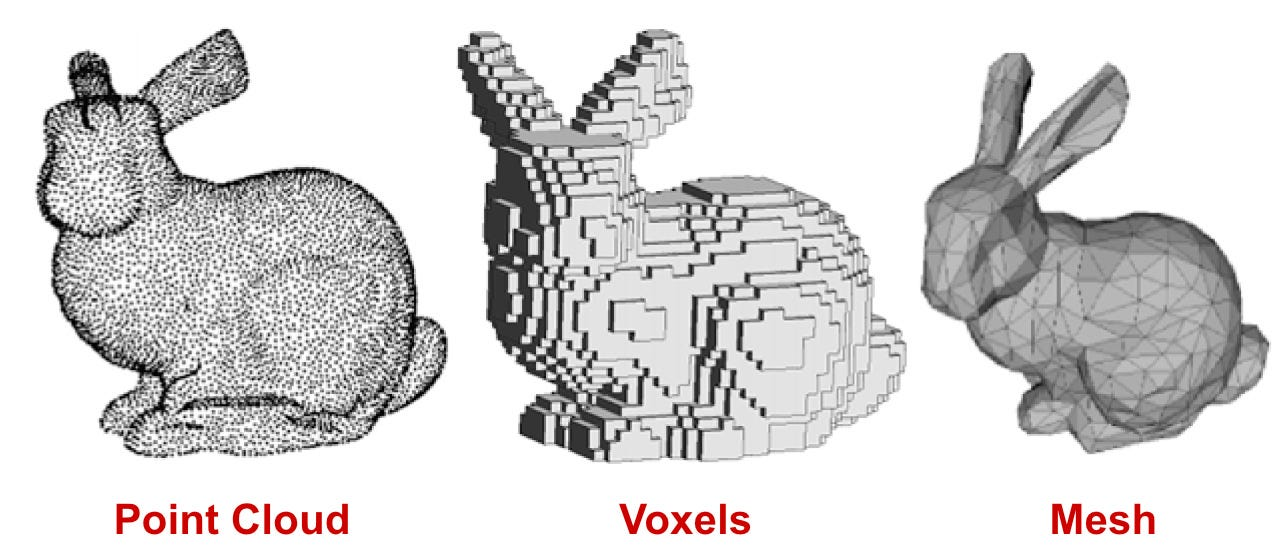
\includegraphics[width=4in,height=1.5in]{MyThesisImages/media/image44.jpeg}
    \caption{Different 3D representations of a rabbit. Source:\cite{wolfe_2023}}
\end{figure}

Due to the complexity of using point clouds as input of GAN models only
a few researchers try and tackle the problem, Point Cloud GAN or PC-GAN
proposed by Chun-Liang Li et al. in 2018 \cite{li_2018_point} was capable of
processing point clouds but despite the impressive results, the model
did not take into account the shape of the object or the relationship
between neighboring point therefore resulting in a suboptimal solution.

The use of point clouds as direct input to deep learning algorithms is
still an under-researched topic. Most implementations of point clouds
use the PointNet \cite{qi_2017_pointnet} that utilizes Multi-Layer Perceptron (MLPs)
and as a result of not using convolution, no relationships of
neighboring points can be found. Ben Hamu et al.\cite{benhamu_2019_multichart} introduced a
model in 2018 to take meshes as input and generate human body and tooth
meshes, based on the progressive growing methodology used in the
ProGAN(2017) model by Karas et al \cite{karras_2017_progressive}. The results are promising
but nowhere near realistic enough.

\begin{figure}[H]
	\centering
    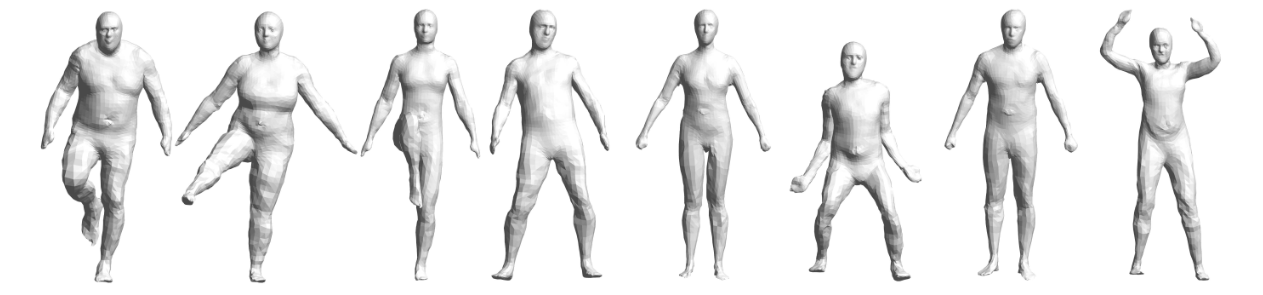
\includegraphics[width=6.26389in,height=1.46528in]{MyThesisImages/media/image45.png}
    \caption{Ben Hamu et al model results. Source:\cite{benhamu_2019_multichart}}
\end{figure}

These problems are leading researchers to convert irregular data into a regular format such as 3D voxel grids which can be used as input to the
convolution architectures. Even though point clouds and meshed do not
have equivalent voxel representation there are a lot of proposals for
conversion to voxels. \cite{yang_2017_3d,kniaz_2019_deep,nozawa_2021_3d}

Wu Jiajun, et al. \cite{wu_2017_learning} demonstrated in their 2017 research that GANs
can be extended to use voxel-based input for training a GAN model to
generate high quality voxelized representations of 3d meshes. Some years
later (2020) Ryan Spick et al. \cite{spick_2020_naive} proposed an extension of the
DCGAN for a 4-channel voxel-based approach for mesh-to-mesh generation
with the inclusion of colors. The important step in their methodology is
the voxelization process of the meshes, they convert all the high
resolution meshes from the initial data set to lower resolution voxel
representations in order to use them as input to the GAN. The proposed
model learns the shape as well as variety of characteristics of
different texture patterns.

\begin{figure}[H]
	\centering
    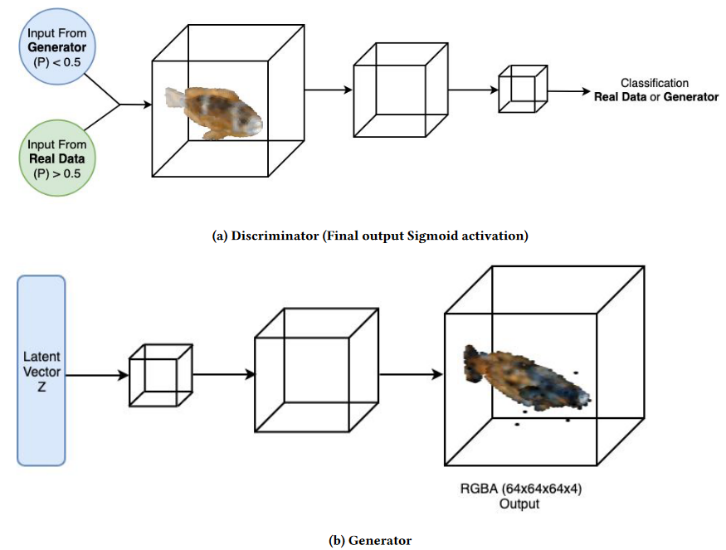
\includegraphics[width=3.29167in,height=2.49524in]{MyThesisImages/media/image46.png}
    \caption{Spick et al. GAN model architecture. Source:\cite{spick_2020_naive}}
\end{figure}


During the data preprocessing to create the voxel representations, every
mesh is placed inside a 64x64x64 voxel grid, and a 3D kernel is run
though the mesh to decide if a voxel should appear or not. The data
could be visualized as RGBA with RGB channels representing the color of
the voxel and the A channel was -1 or 1 depending on if the voxel should
be visible or not in the given position.

The network used was based on the DCGAN model but extended the input by
1 channel, for a total of 3, for the purpose of including the depth. The
network was able to down-sample the 64\textsuperscript{3} to a final
fully connected sigmoid output. The learning rate of the generator plays
an important role in the variety of output produced, a high learning
rate results in lower variation in respect to the training meshes.

\begin{figure}[H]
	\centering
    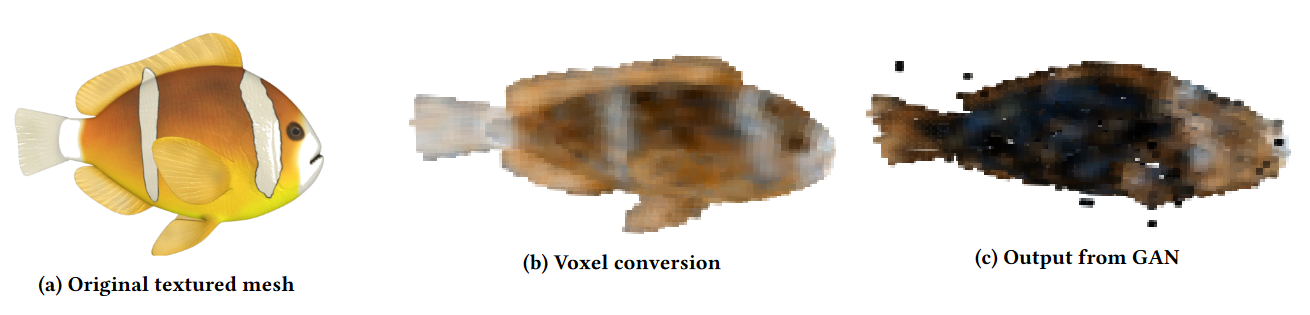
\includegraphics[width=6.25694in,height=1.35814in]{MyThesisImages/media/image47.png}
    \caption{Spick et al. GAN model Results. Source:\cite{spick_2020_naive}}
\end{figure}


After the 3D DCGAN generates the voxel then the next step is converting
that to a mesh as the initial proposition was mesh-to-mesh generation.
The marching cubes algorithm was used to convert the voxel data to a
mesh while preserving the colorization of the model by extrapolating the
voxel RGB values to the corresponding faces.

\begin{figure}[H]
	\centering
    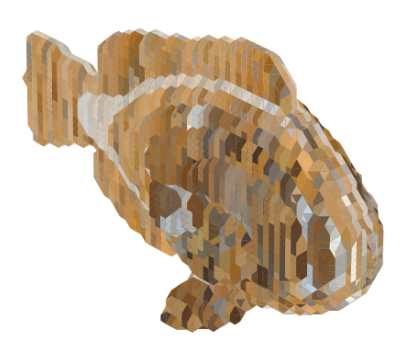
\includegraphics[width=1.99277in,height=1.59306in]{MyThesisImages/media/image48.png}
    \caption{Spick et al. GAN model Results after Marching Cubes. Source:\cite{spick_2020_naive}}
\end{figure}

Due to hardware limitations the results of their model were coarse, by
limiting the voxel grid to 64\textsuperscript{3} lowers the resolution
of the final mesh data produced by the marching cubes algorithm.
Acquiring hardware with more memory would solve the problem and result
in higher quality meshes.

Another approach to produce voxelized representations of 3D objects is
the inverse graphics approach, using 2D images to generate the desired
3D objects. Most proposals on the inverse graphics method require the
use of a Differentiable Rendering. A Differentiable Renderer is
different from a classic industry renderer in the fact that it can
render as well as "De-render", that can be achieved by identifying and
distinguishing the role each input played to result in the final render
frame and thus the name Differentiable.

The problem of differentiability occurs during the rasterization that is
an inherently non-differentiable process in which the renderer must
convert the 3D object to an array of pixels to render on the frame. Only
a handful of handmade Differentiable Renderers are created by the
research community from scratch to overcome the rasterization step. The
video game industry as well as most photorealistic industrial
applications use non-differentiable renderers such as OpenGL, DirectX
and Vulkan, due to their efficiency.

Sebastian Lunz et al. \cite{lunz_2020_inverse} proposed in 2020 an Inverse Graphics GAN
(IG-GAN) model for generating 3D shapes from unstructured 2D image data,
the difference between their approach was that it was aiming to be the
first to utilize a non-differentiable off-the-shelf renderer.

\begin{figure}[H]
	\centering
    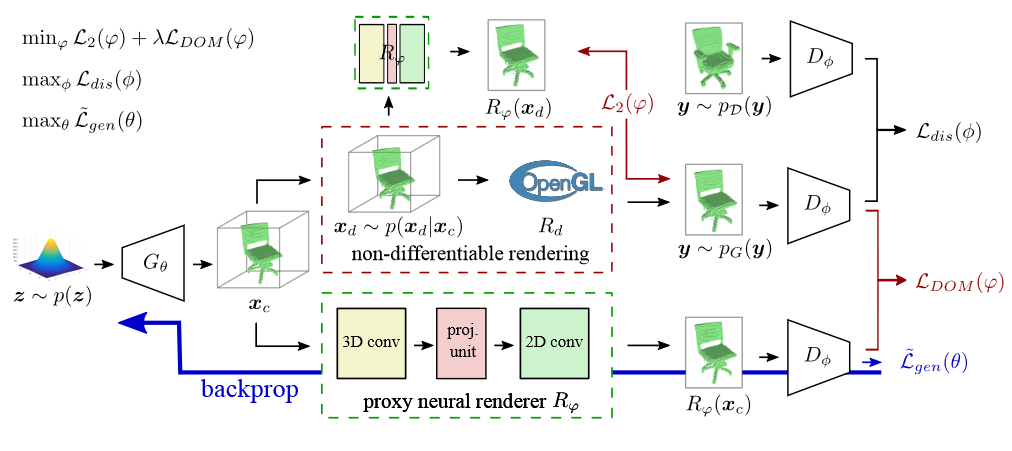
\includegraphics[width=6.25694in,height=2.79167in]{MyThesisImages/media/image49.png}
    \caption{ IG-GAN architecture. Source:\cite{lunz_2020_inverse}}
\end{figure}


The IG-GAN was trained exclusively on 2D data, but they opted to use
voxel-based representation for the 3D object generations. Another
problem in the non-differentiable requirement is that generated objects
are represented as continuous voxel grid, sampling that grid to generate
a mesh is not differentiable, but they can be made differentiable by
representing the occupancy of each voxel by a real number {[}0, 1{]}
which identifies the probability of voxel occupancy.

To fool the discriminator, the 3D generative model must generate
continuous voxel grids which correspond to meaningful representations of
the underlying 3D shapes.

The researchers propose the use of an Intermediate differentiable neural
renderer that will be utilized for backpropagation for the generator's
training to match the output of the off-the-shelf renderer. The
continuous voxel grid representation created by the generator is
rendered as a 2D image by the proxy renderer, furthermore the neural
renderer is trained to minimize the loss of the voxel discretization
process of the continuous voxels.

As discussed previously the Marching Cubes algorithm can be used to
convert the final discrete voxel grid representation but it is apparent
that the output meshes of all the methods showcased are still very low
resolution due to memory limitations, that is should not be a deterrent
as the advancements in super resolution technics and especially 3D super
resolution based on voxel upscaling is impressive. \cite{smith_2018_multiview}

\begin{figure}[H]
	\centering
    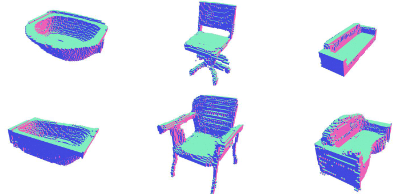
\includegraphics[width=2.6in,height=1.5in]{MyThesisImages/media/image50.png}
    \caption{ Normal maps of objects generated by IG-GAN using multiple images of the same object from different points of view. Source:\cite{lunz_2020_inverse}}
\end{figure}


In conclusion, lets show a complete table comparing all the discussed
approaches in 3D model generation using Generative Adversarial Networks.


\begin{table}[H]
    \centering  
    \begin{tabular}
    {|m{5.5em}||m{2.5em}||m{2.5em}||m{3em}||m{3.2em}||m{2.6em}||m{5em}||m{2.5em}|}
    \hline
         Model & Point cloud Based &Mesh-Based  & Voxel-based &Textured  & Image-to-3D  &Shape \newline Interpolation  & Ouput \\
    \hline
        PC-GAN & Yes & No & No & No & No &Yes  & Point-cloud\\
         \hline
        Hamu\cite{benhamu_2019_multichart} &  No& Yes & No & No & No & Yes &Mesh \\
         \hline
        3D-DCGAN & No & Yes\newline(input) &Yes  & Yes & No & No & Mesh\\
         \hline
        IG-GAN &  No& No & Yes & No & Yes & No & Voxel\\
    \hline
    \end{tabular}
    \caption{Comparison of discussed 3D GAN models}
\end{table} 

\begin{enumerate}
\def\labelenumi{\alph{enumi}.}
\setcounter{enumi}{1}
\item
  \textbf{3D Terrains}
\end{enumerate}

A sub-category of 3D models, terrains are virtual representations of
geographical terrains created by displacing a flat grid of vertices with
a given set of data points.

The most common way for 3d terrain construction with the use of a height
map also known as displacement map, that is a 2-dimensional raster image
of values points which are used to displace a mesh to create
3-dimensional terrain in computer graphics.

\begin{figure}[H]
	\centering
    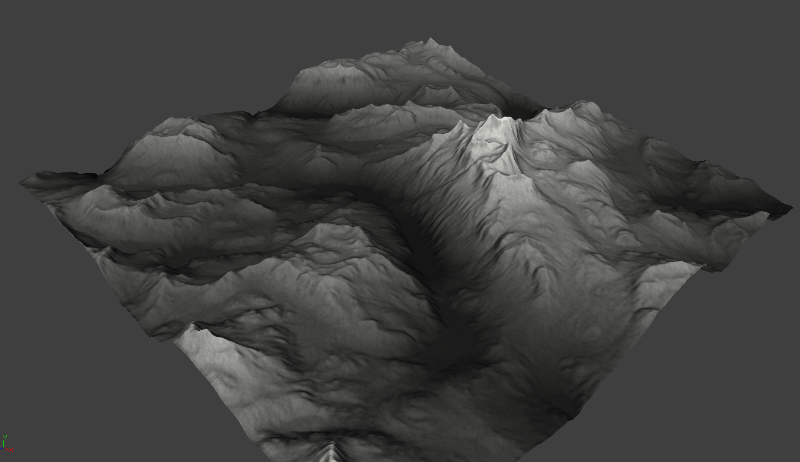
\includegraphics[width=3.63194in,height=2.0921in]{MyThesisImages/media/image51.png}
    \caption{ Terrain rendered from height-map using TerreSculptor.}
\end{figure}

In 2017 a team of researchers proposed an interactive GAN-based model
for terrain authoring using user input in the form of a sketch image
\cite{gurin_2017_interactive}. The basic concept is heavily relying on the data
preprocessing, extracting the specific data from the training data set
of terrains in order to be capable of matching the user input sketches
to terrains and train a conditional GAN to generate a corresponding
terrain.

They implemented 4 different types of models called synthesizers,
"\emph{\textbf{S}} creates a terrain from a sketch containing ridges,
rivers, altitude cues or any combination of the three; the
levelset-to-terrain synthesizer \textbf{L} turns a binary levelset image
into a terrain; the eraser synthesizer \textbf{R} removes a
user-specified part of the terrain and completes it, and, finally, the
erosion synthesizer \textbf{E} transforms an input terrain into the
corresponding eroded terrain."\cite{gurin_2017_interactive}

\begin{itemize}
\item
  In \textbf{S} the sketches are RGB images that have each channel
  representing a specific detail, R is mountain ridges, G is altitude
  ques and B is rivers.
\item
  In \textbf{L} the sketches are black and white images representing the
  part of the terrain with altitude above a threshold (60\%).
\item
  In \textbf{R} the sketches are two channel images, one channel has the
  height map of a terrain and the second channel the parts to be erased,
  the values of first channel are set to 0 where the second channel is
  equal to 1.
\item
  \textbf{E} does not require a sketch; it just runs an erosion
  simulation algorithm on top of a terrain.
\end{itemize}
\begin{figure}[H]
	\centering
    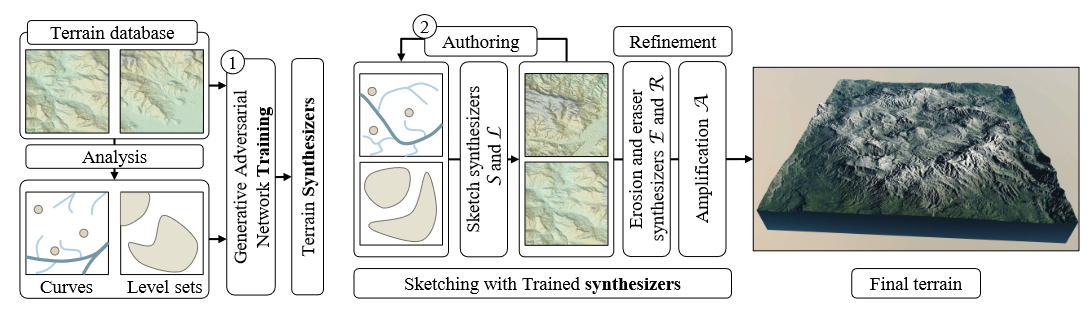
\includegraphics[width=6.25694in,height=1.80556in]{MyThesisImages/media/image52.png}
    \caption{ Eric Guérin et al. terrain model architecture. Source:\cite{gurin_2017_interactive}}
\end{figure}


Artists can use the tool to incrementally generate desired terrains by
providing appropriate input sketches. The sketching process proved to be
very intuitive in both novice and expert artists enabling them to create
realistic terrains parameterized to their desire with minimal effort.
This approach produces very desirable results, but it requires manual
work by the users which may be problematic in many cases requiring vast
amount of input images.

Ryan Spick and James Alfred Walker \cite{spick_2019_realistic} introduced in 2019 a fully
automated approach using the NASA's SRTM data set to train a GAN model
on real world terrain data, satellite images and height maps combined,
to be able to generate realistic variants only with a longitude and
latitude coordinate input that corresponds to a desired region on the
earth's surface. This method did not only generate variants of the
satellite images but also the corresponding height map in order to
generate a ready-to-render textured terrain.

The model works by cropping the terrain data image to 32 random parts in
each iteration and training a SpatialGAN, which is similar to a Deep
convolutional GAN but is non-spatially dependent. They observed that the
was an imbalance between the generator and the discriminator, the
discriminator was getting too good, and the generator could not keep up,
therefore they opted to train the generator twice for every update of
discriminator. Post-process to height map channel of the GAN output was
necessary to remove noise from the training process, structural
similarity was used to choose the median blur kernel size in order to
minimize visual data loss.

A different approach was taken by Panagiotou and Charou \cite{panagiotou_2020_procedural}, two
Greek researchers who used a ProGAN to generate the satellite image
variations and then a pix2pix conditional GAN to obtain the height data,
they also chose to implement the Discriminator with a PatchGAN that
works by classifying patches of the image and then it classifies it by
averaging over all the patches.

The results of this framework are very impressive as the ProGAN approach
is capable of generating variations of high resolution as well as
imitating basic elements like riverbanks, islands with greener water
near the surface and snow.

\textbf{Super-resolution}

It is not uncommon for very successful videogames to get re-released
after many years, these cases are called "Remakes", and they are done
manually by developer studios. This requires huge effort and expense
from the developer's standpoint. AI automated approach to reproduce old
game low resolution texture images in modern day aesthetically appealing
ones would be very helpful.

Many implementations of GANs have been suggested over the years to deal
with the single image super-resolution problem. A group of Chinese
researchers proposed the ESRGAN\cite{wang_2019_esrgan} model, that found popularity as
it was released pre-trained and with easy-to-use code. The model was
based on the SRGAN\cite{ledig_2016_photorealistic} and added many improvements on top of the
base model in order to minimize artifacts and generate representations
closer to the original image. The model makes significant alterations to
the neural network of SRGAN, specifically:

\begin{itemize}
\item
  The Batch normalization layers are removed and replaced with
  Residual-to-Residual Dense Block
\item
  They reimplemented the Discriminator as a Relativistic average GAN
  which learns "whether one image is more realistic than the other"
  rather than "whether one image is real or fake.
\item
  Lastly, they propose an improved version of the perceptual loss by
  using the VGG\cite{grigoryan_2023} features before activation instead of after activation.
\end{itemize}

The ESRGAN model produces very impressive results compared to its
predecessor while being easier to train.

\begin{figure}[H]
	\centering
    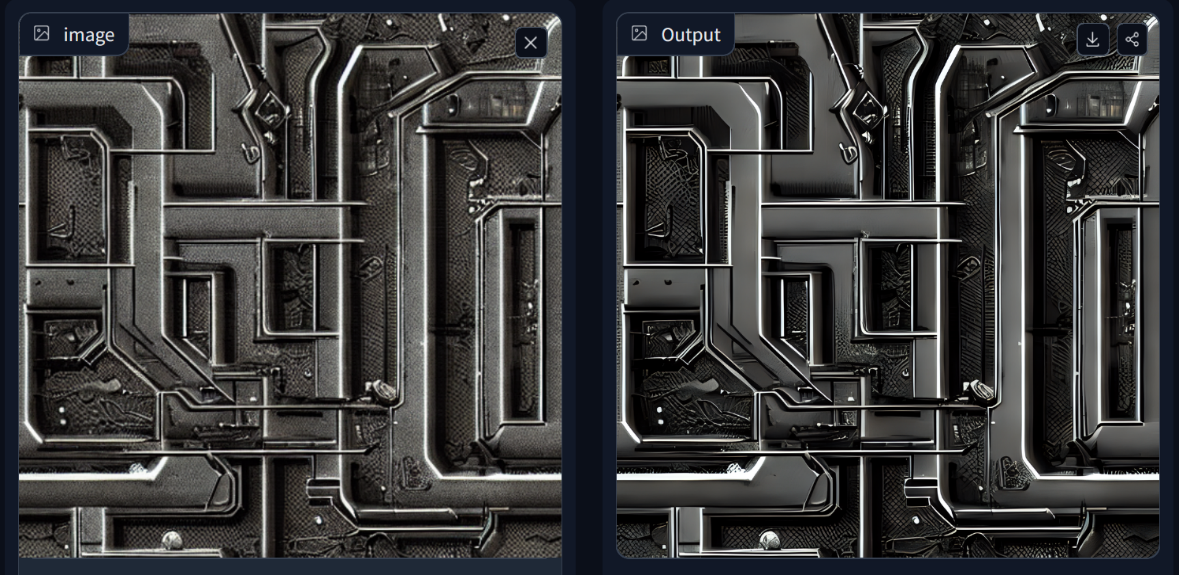
\includegraphics[width=5.35256in,height=2.60169in]{MyThesisImages/media/image53.png}
    \caption{Left original image generated by PolycamAI 512x512. Right 4x upscaled image 2048x2048 using Real-ESRGAN (a free to use online implementation of the ESRGAN model).}
\end{figure}

\subsection{(Section 2.2.c) Latent Diffusion Models}

In previous chapters we discussed various ways to generate synthetic
data, mainly images, with various degrees of success in terms of
quality. VAEs though stable; they perform badly in terms of image
resolution. GANs show promising results but they are unstable during
training and suffer from "mode-collapse", also do not scale well in
more complex multi-modal data distributions.

Researchers in the pursuit of producing higher resolution outputs to
match the current demands have shown that Diffusion-based Models (DM)
were the next step of generative AI. The first attempt that successfully
implemented a model with those requirements was the Jonathan Ho et al.
"Denoising Diffusion Probabilistic Models" \cite{ho_2020_denoising} which proposed a
hierarchical denoising autoencoder architecture.

\begin{figure}[H]
	\centering
    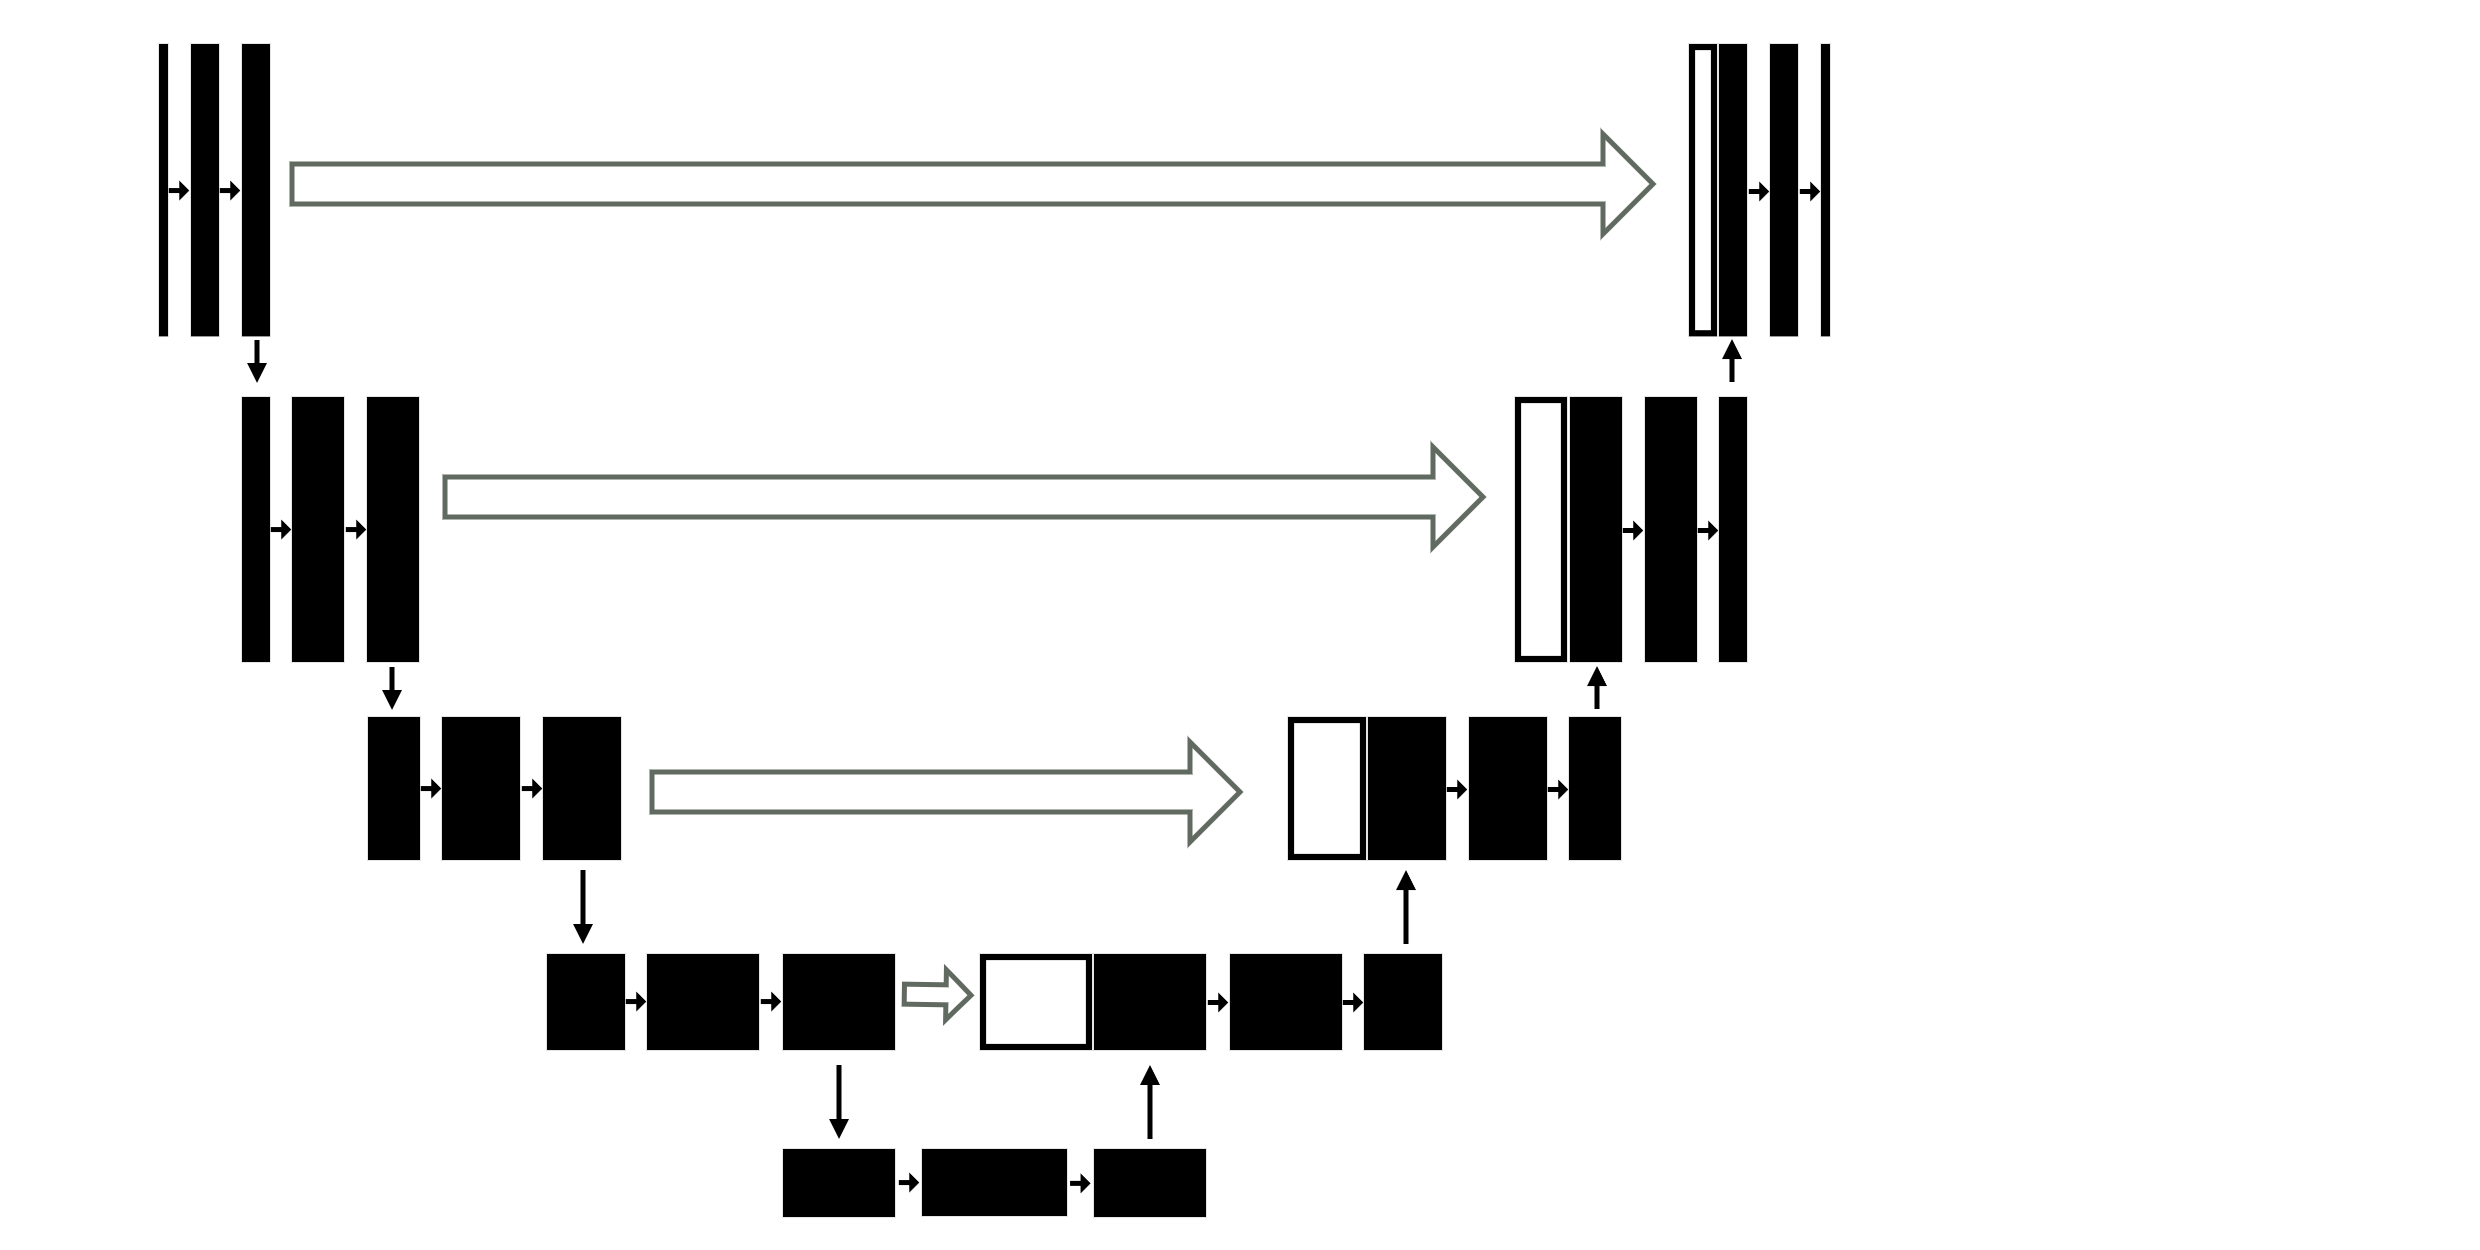
\includegraphics[width=3.07576in,height=1.92793in]{MyThesisImages/media/image54.png}
    \caption{ Simplified example of a Hierarchy of Denoising Autoencoders. Forward process starts from top left and Backward process ends at top right.}
\end{figure}

Not to be confused with variational autoencoders, denoising autoencoders purposely corrupt the input by adding noise of a certain distribution, usually Gaussian, to the data. Mapping the data to a lower dimensional manifold makes the attempt to de-noise more manageable. The corrupting step is called forward process and the de-noising step backward process as it tries to go back to the original non-corrupted data by reversing the mapping learned in the forward process.

In the DM approach, by stacking the denoising autoencoders, the data are
repeatedly corrupted until they have no resemblance to the initial
input, but they become almost entirely a noise distribution. The trained
DM tries to recreate the data by consecutively passing the learned noise
distribution through the backwards process. This results in a highly
compressed mapping of input data and consequently on high resolution
reconstructed variations of that data.

\begin{figure}[H]
	\centering
    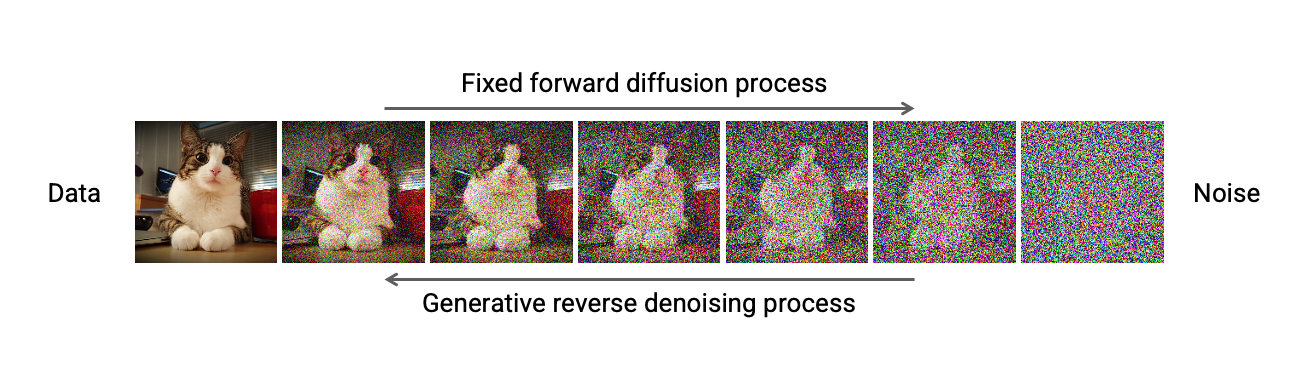
\includegraphics[width=6.25452in,height=2in]{MyThesisImages/media/image55.png}
    \caption{Diffusion process example. Source:\cite{kreis_gao_vahdat_2022}}
\end{figure}

DMs have been shown to produce very impressive results in image
synthesis as well as audio generation. They "belong to the class of
likelihood-based models, whose mode-covering behavior makes them prone
to spend excessive amounts of capacity (and thus compute resources on
modeling imperceptible details of the data." \cite{rombach_2021_highresolution}

Research comparing DM to GANs on image synthesis \cite{dhariwal_2021_diffusion} concluded that
for training the GPU days needed can range from 150 to 1000 V100 for DMs
depending on the size of the dataset and the complexity of the model.
Aiming to mitigate the immense hardware requirements, Rombach et al.
\cite{rombach_2021_highresolution} proposed a latent-based approach to diffusion models. Their
method broke the process down to two steps, the first step was to train
an autoencoder to provide a lower dimensional representation but
perceptually equivalent space, the second step was to train the DMs to
the learned latent space which provides better scaling in respect to
spatial dimensionality. They named this approach as Latent Diffusion
Model or LDM.

\begin{figure}[H]
	\centering
    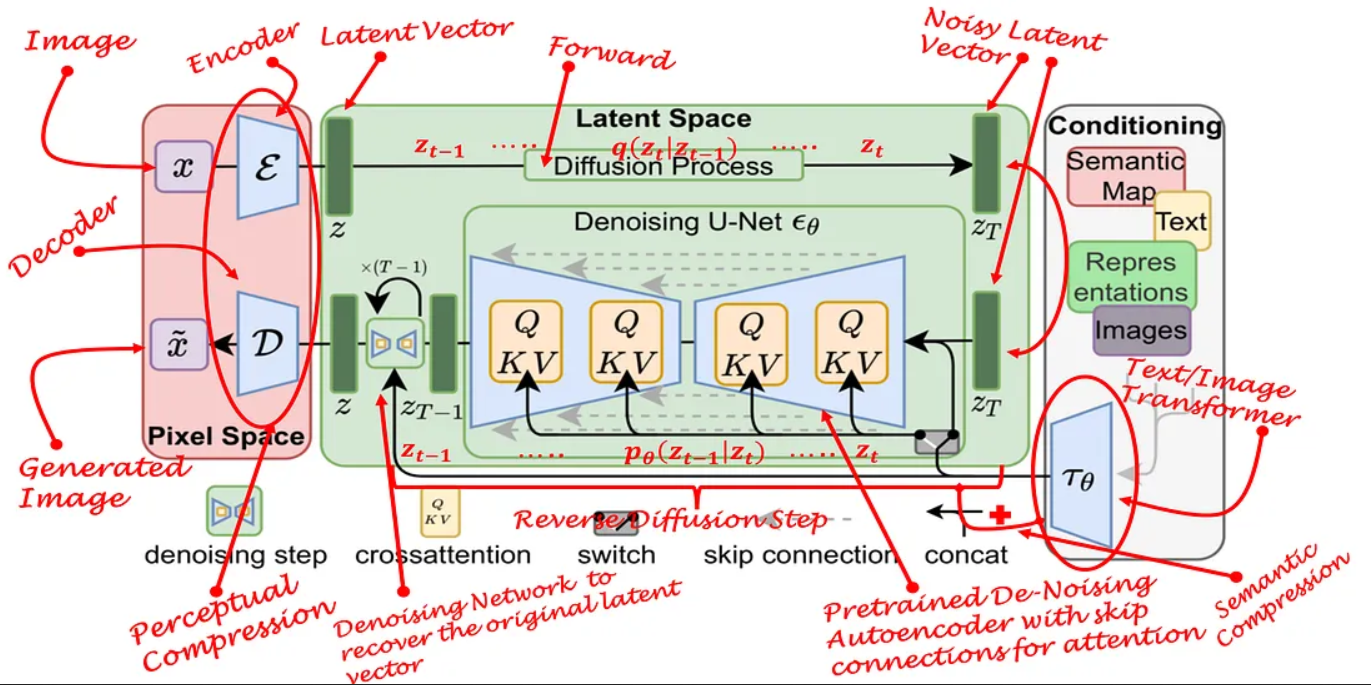
\includegraphics[width=6.2625in,height=3.12847in]{MyThesisImages/media/image56.png}
    \caption{Latent Diffusion Model Architecture with notes. Source:\cite{siddiqui_2022}}
\end{figure}


It is important to mention that the first step of training the universal
autoencoder can be done once and then multiple DMs can be explored for
different tasks. Furthermore, transformers can be connected to the DM in
order to add conditional generation such as text-to-image,
layout-to-image, image-to-image and more.

Advantages of LDMs:

\begin{itemize}
\item
  They lower the computational costs significantly while achieving
  competitive performance on several tasks compared to pixel-based DMs.
\item
  They work at a compression level that retains high levels of detail
  and can reproduce them very accurately.
\item
  They can be used efficiently in higher resolutions in the scale of
  megapixels.
\item
  Capable of densely conditioned generation on large images of 1024x1024
  pixels
\end{itemize}

After the publication of the LDM model many different implementations
hit the scientific community as well as the commercial space for
synthetic image generation, some of the most well-known commercial
models are DALLE2\cite{openai_2022_dalle}, Midjourney \cite{midjourney} and Stable diffusion\cite{stable_Diff}.

DALLE2 was released on April 6, 2022, which was their second attempt at
an image generative model after the first DALLE released on January 5,
2021. DALLE2 is an LDM based model compared to its autoregressive
predecessor and boasted very impressive results in comparison.

Midjourney is a small independent research lab created by David Holtz.
They developed Midjourney AI and released it July 12, 2022, which is
their variation of an image generation LDM and is implemented on top of
the popular Discord community platform \cite{discord_2024_discord}.

Stable Diffusion was developed by a research group from the University
of Munich along with researchers from the Runway AI, an American based
company. The project received support from many non-profit organizations
in terms of donations as well as all the training data used. An
important contributor was Stability AI that offered computational
resources to the project and the final model was released in August 2022
with the name Stable Diffusion.

Stable Diffusion is a latent diffusion model similar to the other two
mentioned above but there is a very important distinction that makes it
a special case, the code as well as the trained weights of the model are
open source and free for public use. The model can be run natively on a
user's computer with the requirement of a GPU with at least 4gb VRAM,
that was an important feature due to all other competitors relying
solely on online cloud services.

\begin{table}[H]
    \centering  
    \begin{tabular}
    {|m{7em}||m{5em}||m{5em}||m{5em}|}
    \hline
         &DALLE2   &Midjourney	&Stable \newline Diffusion \\
    \hline
         	 
Text-to-image	&Yes	&Yes	       &Yes\\
\hline
Image-to-text	&No	    &Yes	       &No\\
\hline
Image-to-Image	&Yes	&Yes	       &Yes\\
\hline
In-painting	    &Yes	&Yes	       &Yes\\
\hline
Out-painting	&Yes	&Yes	       &Yes\\
\hline
Animate images	&No	    &No	           &Yes\\
\hline
Image-to-Video	&No	    &No	           &Yes\\
\hline
Text-to-Video	&No	    &No	           &Yes\\
\hline
Image Blend	    &No	    &Yes	       &No\\
\hline
Seamless Image	&No	    &Yes	       &No\\
\hline
Super Resolution &Yes (limited 1024x1024)	&Yes	&Yes\\
    \hline
    \end{tabular}
    \caption{List of most important features of the three discussed
models. Stable diffusion is clearly more advanced in terms of features
due to the open-source nature of the project.}
\end{table} 
 

\paragraph{3D OBJECTS\\}

Latent diffusion models are not confined only in image synthesis even
though they were developed with that in mind, they can be applied in
other tasks that require high-resolution precise output such as audio
synthesis and 3D shape generation.

As discussed in length on the previous section, GANs have been used
successfully for 3D shape generation but the results are novel and might
possibly serve as prototypes in actual commercial cases, due to the lack
of detail fidelity. LDMs come to the table bringing efficient big data
computational capabilities making them the next step in high resolution
and complexity applications such as 3D shape generation.

Compared to GAN models falling short in understanding high resolution
point cloud representations LDMs can model highly complex distributions
and don't suffer from mode collapse as they are likelihood-based
probabilistic models and have been shown to produce great results in 3D
object synthesis.

Luo and Hu \cite{luo_2021_diffusion}, inspired by thermodynamics, proposed an LDM in 2021
capable of generating 3D shapes in point cloud representation. The model
was based on a non-equilibrium thermodynamic system in contact with a
heat bath, the point cloud was seen as particles inside the system that
under the effect of the heat bath disperse and diffuse through the
entire space. By simulating this diffusion process, the researchers
converted the initial point cloud distributions to simple noise
distributions by adding noise in each time step. Consequently, the point cloud generation would coincide with the reverse diffusion process.
\begin{figure}[H]
	\centering
    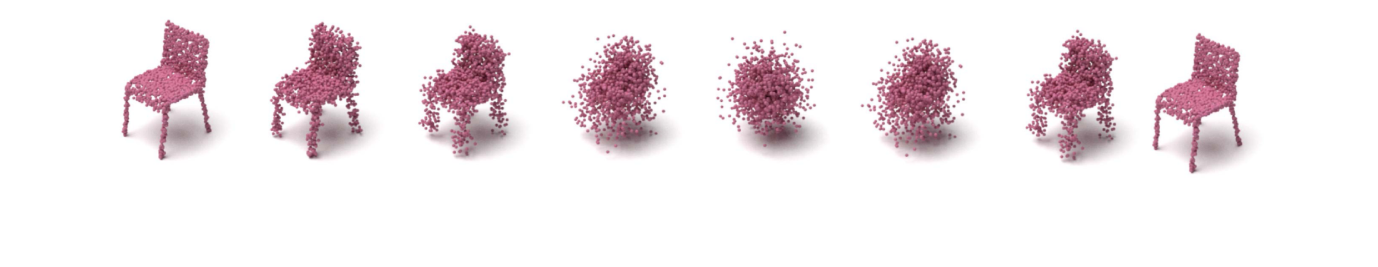
\includegraphics[width=6.25482in,height=1in]{MyThesisImages/media/image57.png}
    \caption{3D point cloud diffusion. Source:\cite{luo_2021_diffusion}}
\end{figure}


This reverse diffusion is modeled as a Markov chain with the objective
of converting the initial distribution to a target distribution, thus
the goal of the LDM is to learn the transition kernel so the chain can
reconstruct the shape. The Markov chain alone is not capable of
reconstructing multiple shapes, for that purpose a shape latent variable
is introduced as a condition to the kernel. This shape latent is learned
end-to-end in the autoencoder step via normalizing flows
parameterization. The training objective of the model is to maximize the
variational lower bound of the likelihood of the point cloud conditional
on the shape latent.

The model shows very promising results in shape reconstruction as well
as latent space interpolation between two different point clouds,
notably when trained on the entire ShapeNet dataset \cite{shapenet} it was
shown to outperform all other competition (AtlasNet \cite{groueix_2018_atlasnet}, PointFlow
\cite{yang_2019_pointflow}, ShapeGF \cite{cai_2020_learning}, suggesting LDMs have higher capacity to
encode different shapes.

Zhou et al. \cite{zhou_2021_3d} proposed a Point-Voxel hybrid LDM (PVD) capable not
only of 3D shape generation but also multimodal shape completion, making
a huge step forward in generated variations. The PVD model utilizes as
its backbone the Point-Voxel CNN \cite{liu_2019_pointvoxel} that voxelizes the point cloud
data for 3D convolution, aiming to exploit the strong spatial
correlation inherent in point cloud data.

The shape generation part of the model is very similar to Luo and Hu
that was discussed previously, the important addition and a very
desirable feature is the multi-modal shape completion. Most
implementations follow an encoder-decoder architecture for shape
completion that offers a deterministic result and therefore only a
single possible completed final shape. PVD on the other hand adopts a
probabilistic approach on shape completion and can generate many
probable variations of a shape from an initial observation of a partial
set of points as well as from a single-view depth-map. In the case where
it is provided with a depth map, the model converts it to a partial
point cloud representation. The partial is named z0 and it remains
unchanged throughout all the time steps, only the missing parts are
diffused.

\begin{figure}[H]
	\centering
    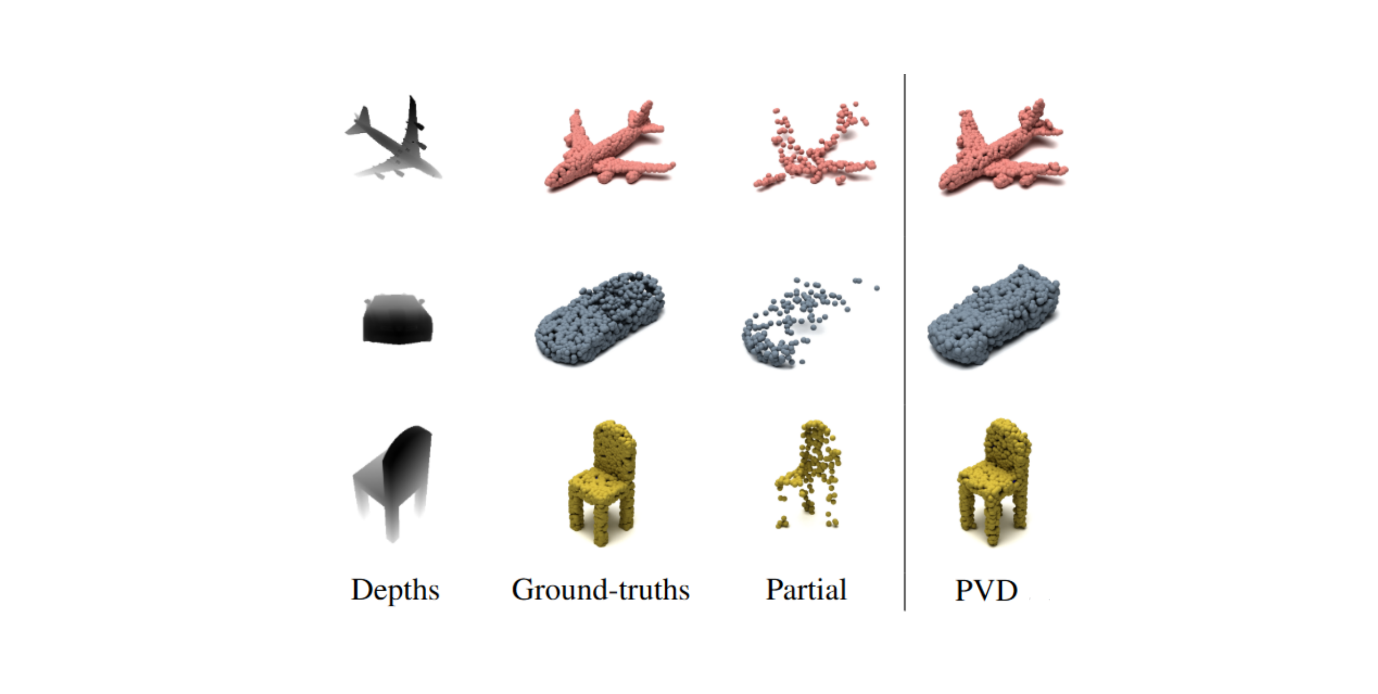
\includegraphics[width=6.25589in,height=2.36522in]{MyThesisImages/media/image58.png}
    \caption{Partial point clouds from depth map and PVD completed shape. Source:\cite{zhou_2021_3d}}
\end{figure}

\begin{figure}[H]
	\centering
    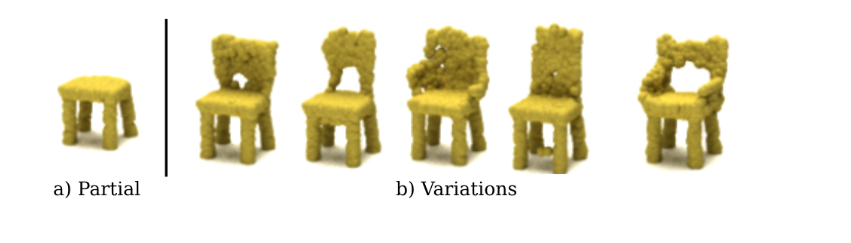
\includegraphics[width=6in,height=1.50256in]{MyThesisImages/media/image59.png}
    \caption{ a) partial point cloud b) Possible variations. Source:\cite{zhou_2021_3d}}
\end{figure}


Both the Zhou et al as well as Luo and Hu models show very promising
results but they both suffer from the same problem. Point cloud and
voxel representations are mostly useful for research purposes, the
artistic community as well as the commercial industry prefer working
with smooth high resolution mesh representations as they coincide with
their preferred workflow.

A group of researchers in collaboration with Nvidia, University of
Toronto and the Vector Institute proposed in 2022 \cite{zeng_2022_lion} a framework
aiming to fulfill multiple criteria and create a useful tool
corresponding to the needs of digital artists. The model is called Latent
Point Diffusion Models for 3D shape generation or LION for short and is
structured as a variational autoencoder (VAE) with a hierarchical latent
space that combines a vector-based global shape latent representation
with a point-structured latent space, along with two denoising diffusion
models (DDM) trained in those latent spaces.

The training process involves a two-stage process, in the first stage
the model is trained as a regular VAE, trying to maximize the ELBO and
in the second stage the encoder and decoder networks of the VAE are
frozen and two different DDMs are trained one on the shape latent space
and another on the point cloud latent space. The implementation of the
model's encoder, decoder and point cloud DDM is based on the Zhou et al.
approach using the Point-Voxel CNN. The shape latent DDM uses a ResNet
\cite{he_2016_deep} which is a type of convolution network with fully connected
layers.

One of the main objectives of LION is flexibility in real time
conditional generation, the VAE approach enables the model to be adapted
for various tasks without the need for retraining the DDMs. LION can be
guided by multiple input methods:

\begin{itemize}
\item
  Low resolution voxel grid
\item
  Single view RGB image
\item
  Text
\end{itemize}

\begin{figure}[H]
	\centering
    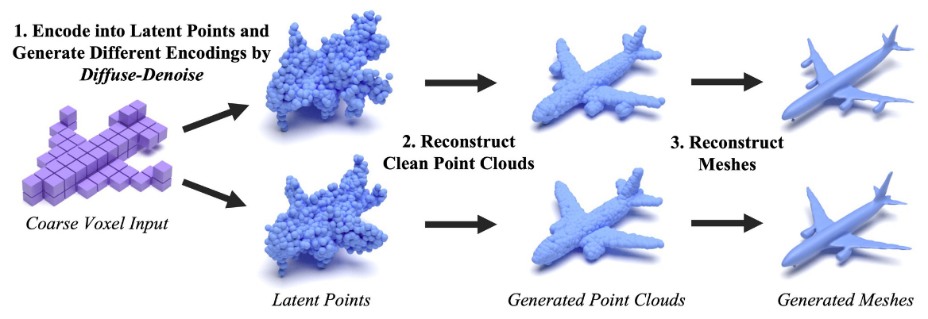
\includegraphics[width=4.20513in,height=1.44792in]{MyThesisImages/media/image60.png}
    \caption{ LION same voxel input resulting in different final
generations. Source:\cite{zeng_2022_lion}}
\end{figure}

Furthermore, the model is capable of multimodal shape generation
providing a variety of generated outcomes for the same object as well as
shape interpolation between two different objects.

The defining feature of LION is the implementation of a state-of-the-art
surface reconstruction technic in order to provide the end user with a
desirable mesh representation instead of a voxel or a point cloud. The
method used is called "Shape as Points" (SAP) \cite{peng_2021_shape} and is based on
differentiable Poisson surface reconstruction that can be trained on
noisy point cloud data. The SAP is topology agnostic and is further
fine-tuned on point clouds generated by LION by encoding "clean"
shapes and denoise-diffuse them only a few times so that no details are
lost but the noise generated resembles that of a LION generated shape.

\begin{figure}[H]
	\centering
    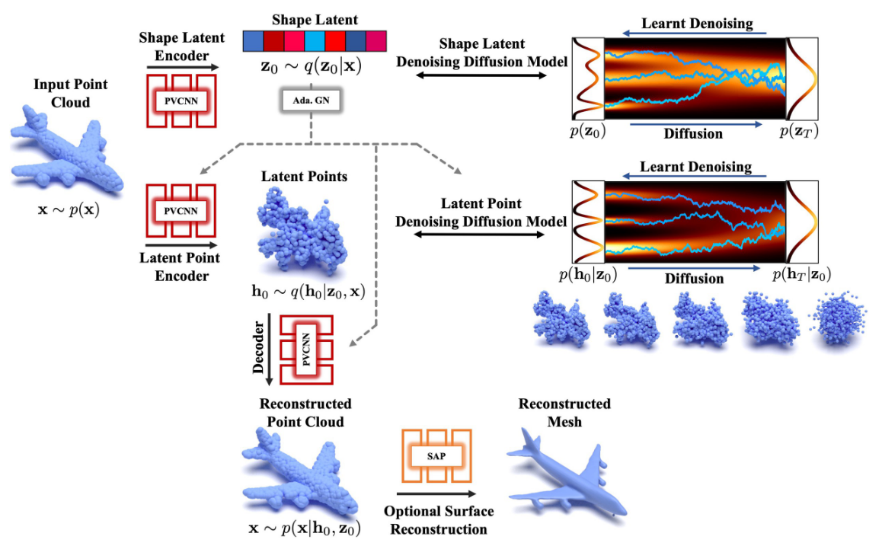
\includegraphics[width=5.03976in,height=3.12121in]{MyThesisImages/media/image61.png}
    \caption{ LION Architecture. Source:\cite{zeng_2022_lion}}
\end{figure}

\begin{table}[H]
    \centering  
    \begin{tabular}
    {|m{2.2em}||m{3em}||m{2.7em}||m{2.2em}|m{2.2em}||m{4.7em}||m{5em}||m{2.8em}||m{2.8em}|}
    \hline
    Model	&RGB-D Input	&RGB Image Input	&Voxel Input	&Text Input	&Partial\newline Completion	&Shape\newline Interpolation	&Mesh Output	&Point Cloud Output\\
    \hline
         	
PVD     &Yes	&No	    &No	    &No	    &Yes   &Yes	   &No     &Yes\\
\hline
LION	&No	    &Yes	&Yes	&Yes	&No	   &Yes    &Yes    &Yes\\
 
    \hline
    \end{tabular}
    \caption{Comparison of PVD and LION models.}
\end{table} 

\textbf{{AUDIO}}

There are two main ways of seeing audio in digital format, in waveform
and in Musical Instrument Digital Interface (MIDI). The waveform is a
graph representation of an analog audio signal as a function over time,
"where the magnitude of the signal is sampled regularly at uniform
intervals, then quantized to a series of symbols in a digital (usually
binary) code"\cite{LCPM}.  The MIDI format is a protocol developed for
musical tool communication, it does not make sound, it is a symbolic
representation of musical notes and different pitches that can be
interpreted by a corresponding MIDI instrument or software. \cite{instructables_2012_what}

\begin{figure}[H]
	\centering
    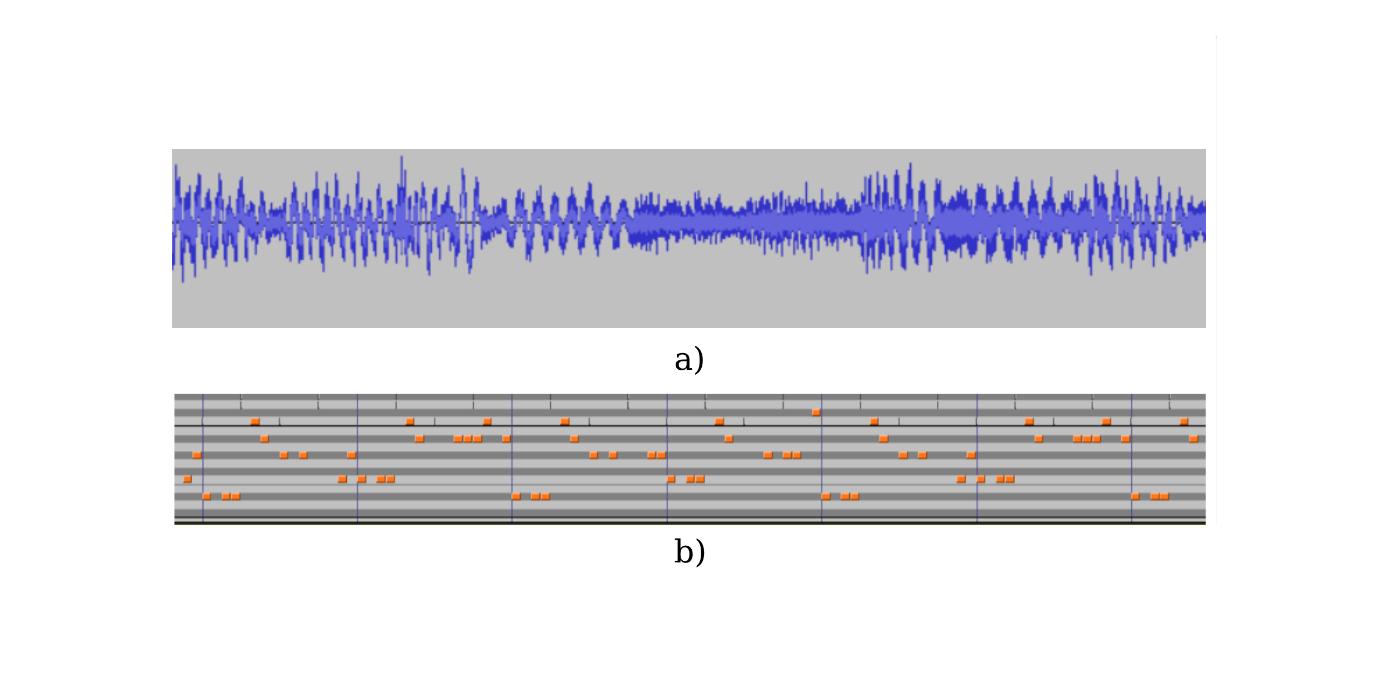
\includegraphics[width=4.73077in,height=1.92218in]{MyThesisImages/media/image62.png}
    \caption{ Example of a) Waveform b) MIDI representation.}
\end{figure}

The research community has proposed methods of generating audio using
both formats as inputs for training latent diffusion models with various
degrees of success. Mittal et al. \cite{mittal_2021_symbolic} made a proposal in 2021 for a
symbolic music generation model trying to tackle the problem using MIDI
audio samples as they offer many advantages over traditional waveform.

Their model utilized a VAE to encode the discrete MIDI input to a
continuous latent space where a diffusion model will be trained on, more
specifically they opted to use the pretrained 2-bar MusicVAE \cite{roberts_2018_a}
which uses bidirectional recurrent neural networks for the encoder and
an autoregressive decoder. The model was trained with the Lakh MIDI
Dataset (LMD) \cite{raffel_2016_learningbased} containing over 170,000 MIDI files, each file was
comprised of 1024 discrete tokens that were divided to 32 parts and fed
to the MusicVAE encoder in order to produce 32 continuous latent
variables that will be fed to the diffusion model.
\begin{figure}[H]
	\centering
    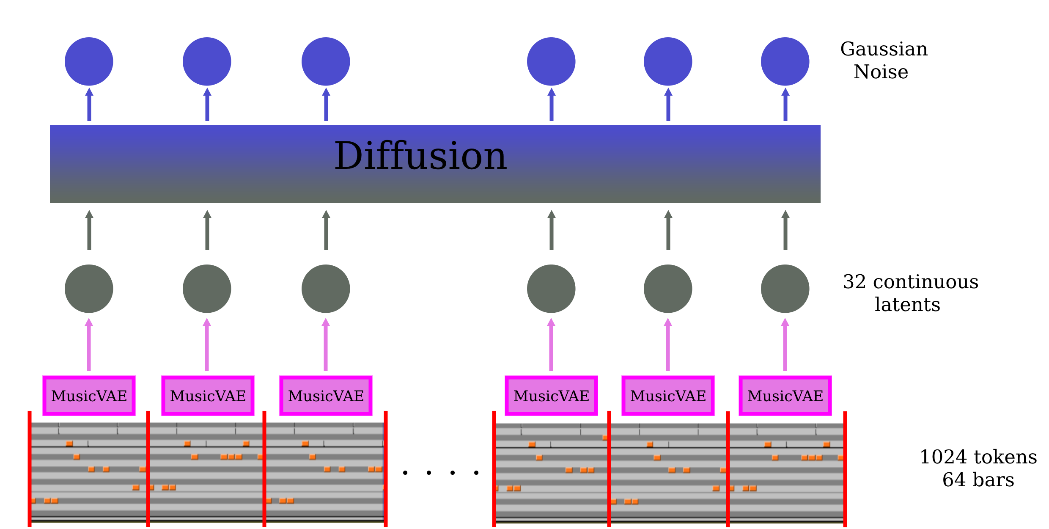
\includegraphics[width=4.73718in,height=2.38831in]{MyThesisImages/media/image63.png}
    \caption{MIDI latent diffusion model Architecture.}
\end{figure}

This multi-stage model is capable of unconditional MIDI music generation
as well as conditional infilling. To demonstrate conditional infilling
of latent embedding in an unconditionally trained diffusion model the
researchers remove from the total 32 sections the 16 middle ones,
leaving only 8 on the start and 8 on the end of the MIDI sample for the
purposes of generating the missing sections by conditioning the model on
those remaining 16.

Despite the promising results in MIDI audio synthesis demonstrated by
Mittal et al., there are no practical applications apart from the
infilling which is still limited with no way of guided generation, due
to the unconditional nature of the model. Most recent audio generation
approaches focus on text guided generation but have moved away from the
symbolic MIDI format and focus on the classic waveform representation.

Research in previous years focused on labeled audio data, but the
quantity of those data was limited to a small set of labels like the 10
different sound classes in the UrbanSound8K \cite{2019_urbansound8k} dataset, resulting
in limited flexibility and quality of the generated results along with
high computational costs. AudioLDM \cite{liu_2023_audioldm} proposed by a team of
researchers and showcased in the Hawaii International Conference on
Machine Learning in 2023, focusing on natural language text descriptions
of audio data in order to guide the diffusion model.

The AudioLDM model uses a mel-spectrogram-based VAE along with
contrastive language-audio pretraining (CLAP)\cite{wu_2022_largescale} embeddings for
latent variable generation. By leveraging the audio-text-aligned
embedding space in CLAP, paired audio-text data are not required during
training of the LDM. Along with audio generation the model can achieve
text-guided audio style transfer, super-resolution, and inpainting,
without fine-tuning.

\begin{figure}[H]
	\centering
    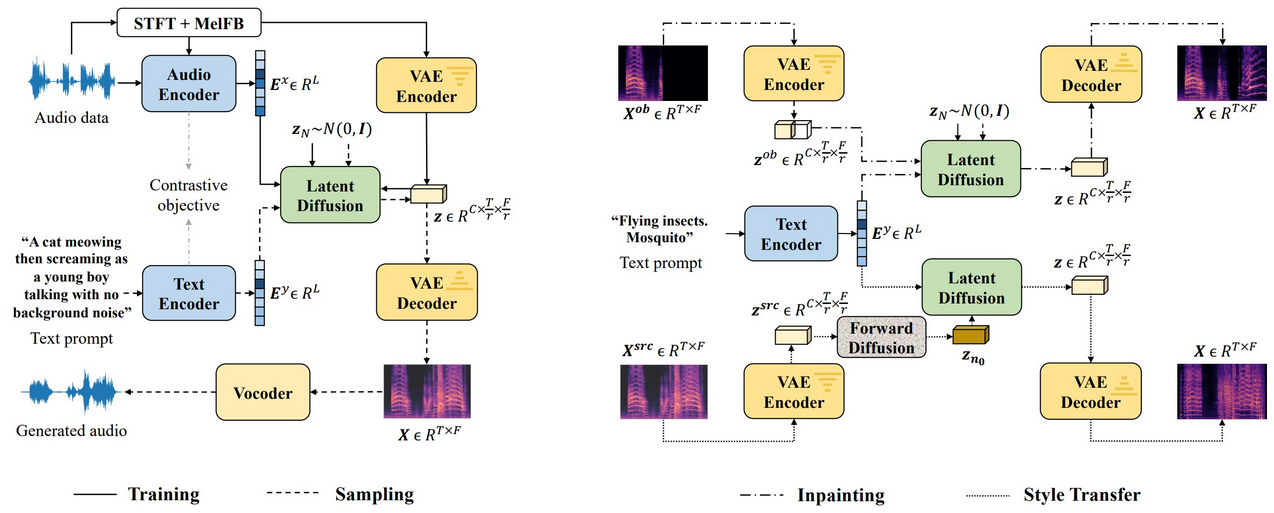
\includegraphics[width=6.25625in,height=2.51944in]{MyThesisImages/media/image64.png}
    \caption{AudioLDM Architecture. Source:\cite{liu_2023_audioldm}}
\end{figure}

The audio encoder is based on HTS-AT\cite{chen_2022_htsat} which is a hierarchical
token-semantic audio transformer used for sound classification and
detection and the text encoder is based on RoBERTa \cite{liu_2019_roberta}, an improved
version of the BERT model used for language pretraining. Text-To-Audio
(TTA) requires generation of compositional audio that is consistent with
the text descriptions provided in natural language, but the datasets are
not large enough to achieve desirable results. AudioLDM uses the
AudioGEN\cite{kreuk_2022_audiogen} method which mixes pairs of audio samples and
concatenated the textual context for the purpose of creating new paired
data, thus increasing the size of the dataset significantly. As mentions
previously AudioLDM uses audio only conditioning for the LDM and as a
result increasing the audio samples with this mix-up process results
increased robustness to CLAP embeddings and at the same time removing
the need for language-audio paired data.

The decoder of the model takes the generated compressed latents and
transforms them to a mel-spectrogram representation which is then used
as input to a vocoder. This vocoder is responsible for transforming the
mel-spectrogram generated by the LDM to a waveform representation, it is
implemented using the Hifi-GAN \cite{kong_2020_hifigan} trained on the AudioSet \cite{audioset}
dataset. The GAN has two sets of discriminators, a multi-period
discriminator, and a multi-scale discriminator and is widely used for
speech waveform generation due to the enhanced perceptual and generated
waveform quality.

Experiments done with AudioLDM show great flexibility and versatility in
a large number of cases as well as comprehensive understanding natural
language textual input for guided generation of synthetic audio.
\newline\newline
List of AudioLDM capabilities:

\begin{multicols}{2}
\begin{itemize}
\item
    Text-to-Audio Generation
\item
    Audio Style Transfer
\item   
    Audio Super-Resolution
\item    
    Audio Inpainting
\item    
    Environment Control (e.g. huge room, studio etc.)
\item
	Music Generation
\item
	Music Control (e.g. instruments)
\item	
    Pitch Control
\item    
	Material Control (e.g. “hit wood”, “hit metal”)
\item	
    Temporal Order Control

\end{itemize}
\end{multicols}

Although impressive, AudioLDM has limitations in the audio sample
quality and length, all the audio used in training the model is
resampled to 16khz mono format and length of 10 seconds. Another problem
of the model is that it is not fine-tuned end-to-end, all the subsystems
are trained independently which may result in module misalignment. For
example, the VAE may not learn an optimal latent space representation
for training the LDM. Moreover, there is no filter for sensitive
language context and abusing the model's capabilities can result in
creation of harmful audio content or misleading information.

With the recent revolution of large language models (LLM), zero- or
few-shot performance in natural language processing has increased
significantly. Inspired by the LLMs and the AudioLDM model Ghosal et al.
\cite{ghosal_2023_texttoaudio} from the University of Singapore proposed a large language
based TTA model named TANGO, improving upon the existing AudioLDM
approach in two aspects. The first improvement is the removal of the
CLAP-based text-encoder and replacement with the FLAN-T5\cite{chung_2022_scaling} which
is initialized with a T5 checkpoint and fine-tuned on instructions and
chain-of-thought reasoning. The second improvement came in the audio
data augmentation with the mix-up technique, instead of random audio
pair mixing the TANGO model inspired by Tokozume et al.\cite{tokozume_2018_learning},
considered a pressure-level consideration in the mixing process in order
to avoid high-pressure loud audio to be mixed with low-pressure quitter
samples which would result in the latter being overwhelmed and get
drowned. Moreover, the energy of a sound wave which is proportional to
the square of the amplitude is also considered for the mixing step.

\begin{figure}[H]
	\centering
    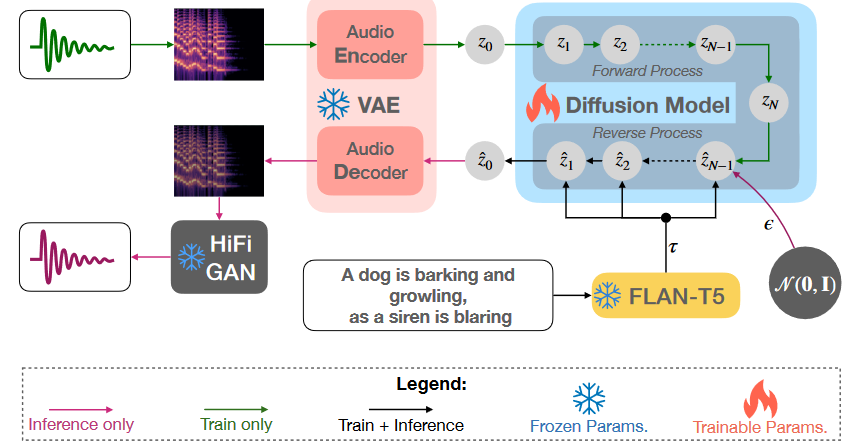
\includegraphics[width=3.89744in,height=2.0425in]{MyThesisImages/media/image65.png}
    \caption{TANGO Architecture. Source:\cite{ghosal_2023_texttoaudio}}
\end{figure}

The LDM used in TANGO is trained in paired text-audio data from the
AudioCaps\cite{kim_2019_audiocaps} dataset instead of using exclusively audio data like
AudioLDM. The dataset is 45,438 audio clips with length of 10 seconds
each, paired with 5 different human-written captions. Tango achieves
better or comparable performance in metrics with a dataset of samples 63
times smaller than that needed to train AudioLDM.

Nevertheless, regardless of all the improvements in terms of data
efficiency and a more comprehensive LLM offering more nuanced natural
language processing, TANGO still has some inherent limitations, firstly
the size of the dataset limits the model ability to corelate text input
to audio in a highly precise degree, slightly different prompts can
result in very similar generated audio output. As demonstrated by the
researchers "Chopping tomatoes on a wooden table" and "Chopping
potatoes on a metal table" are very similar and due to limited size of
the training data TANGO does not have the ability to differentiate
between materials like the AudioLDM, which could be solved by training
the model in larger datasets. Secondly TANGO follows in the steps of
AudioLDM in the Hifi-GAN vocoder module, therefore the quality of the
output is limited to 16khz which might be enough for novel uses but is
low quality for digital audio professional applications.

The next improved implementation of AudioLDM called AudioLDM2\cite{liu_2023_audioldm2}
comes to introduce a "language of audio" (LOA), which is a sequence of
vectors that represent the semantic information of an audio clip. This
approach allows a universal representation of audio, which enables
large-scale self-supervised pretraining of the core latent diffusion
model without audio annotation and helps to combine the advantages of
both the autoregressive and the latent diffusion model.

AudioLDM2 utilized the CLAP audio encoder like its predecessor, combined
with 3 other modules, FLAN-T5 to capture additional temporal data, a
Phoneme Encoder for encoding textual input into phonemes which is a
widely used module in text-to-speech applications and ImageBind which is
similar to CLAP but with more embedded modalities in order to condition
the model in image, video, depth map, thermal images and inertia
measurement units. All this conditioning information is translated to
LOA using GPT-2 initialized with pretrained weight and fine-tuned on the
conditioning information and ground truth data.

Instead of using a hand-build VAE, this time they opted for AudioMAE
which is an extension of the image-based masked autoencoder architecture
but conditioned to learn audio spectrogram representations from
unlabeled audio data without relying on manually labeled annotation.
First the audio is converted to a mel-spectrogram and then it is encoded
to patches with a high masking ratio, feeding only the non-masked tokens
through encoder layers. The decoder then re-orders and decodes the
encoded context padded with mask tokens, in order to reconstruct the
input spectrogram.

\begin{figure}[H]
	\centering
    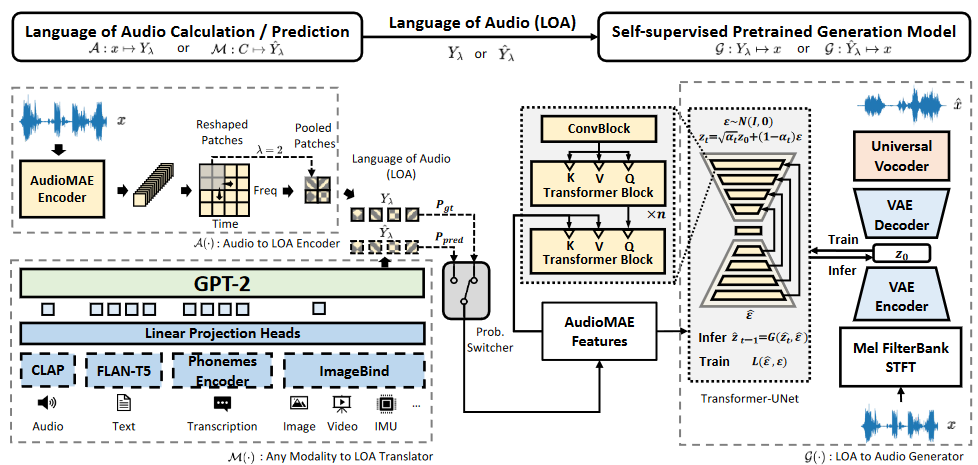
\includegraphics[width=5.55769in,height=2.63956in]{MyThesisImages/media/image66.png}
    \caption{AudioLDM2 Architecture. Source:\cite{liu_2023_audioldm2}}
\end{figure}


The LDM part of the model does not use the AudioMAE\cite{huang_2022_masked} latent
representation because it is not focused on reconstruction quality and
has a low compression rate. On the other hand, the VAE architecture
shows better spectrogram reconstruction ability and higher compression
rate making it better for training the diffusion model.

The AudioLDM2 model shows state of the art results in text to audio,
text to music and text to speech applications, although it is trained on
resampled 16khz audio in order to compare with previous models, it is
capable of generating 48khz mono audio.

Generating audio of high quality is very computationally demanding,
that's why the models we discussed so far focus on 16khz mono samples.
Also, another problem is the length of audio samples used to train the
model, the input samples will determine the final generated audio
length, training on 10 seconds samples will result in generating 10
seconds audio clips. Another approach to TTA generation is proposed by
Evans et al.\cite{evans_2024_fast} moving away from LLM for text input and focusing
on quality and length of the generated audio output. They proposed a
model named Stable Audio, capable of generating 44.1 kHz long-form
variable length stereo audio with maximum of 95 seconds which
revolutionized the TTA capabilities.

Following the specification of commercial standard audio, 44,1khz
stereo, Stable Audio introduces TTA using timing embeddings for the
purpose of generating audio of variable length depending on the desired
time input. It uses two timing variables "seconds\_start" and
"seconds\_total", during training chunks of 95 seconds from longer
clips can be used by correctly aligning the 95 seconds window using the
seconds\_start. In practice, the model always generates 95 seconds of
audio, it uses the seconds\_start variable set to 0 and the
seconds\_total set to whatever second the user chooses, then pads the
rest with silence and at the end cuts the clip to the desired
seconds\_total, achieving variable length generation.

\begin{figure}[H]
	\centering
    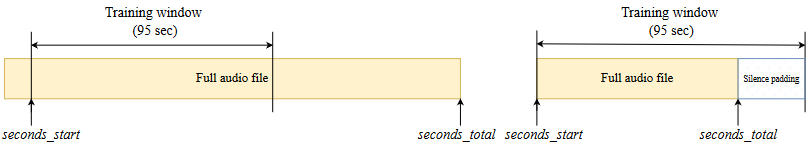
\includegraphics[width=6.25625in,height=1.13472in]{MyThesisImages/media/image67.png}
    \caption{Stable Audio timing variables. Source:\cite{evans_2024_fast}}
\end{figure}

Stable audio uses CLAP embeddings for textual conditioning, a VAE model
based on Descript Audio Codec\cite{kumar_2023_highfidelity} but removing the quantizer
module and utilizing Snake activations for improved audio reconstruction
and an LDM implementation focused on high memory-efficiency attention
layers in order to scale more efficiently with longer sequences.

Regarding training data, the model is using the AudioSparx \cite{AudioSparx}
provider with corresponding metadata for each sample. For prompt
preparation the model used random concatenation of those metadata which
include natural language descriptions as well as audio specific
attributes such as genre, mood, tempo Beats Per Minute and instruments
used per sample.

Stable audio is able to generate state of the art audio with the
relatively small dataset, and is capable of generating high quality
stereo music, sound effects and specific instruments with considerably
less inference time compared to it equivalent competitor AudioLDM2
model.


\begin{table}[H]
    \centering  
    \begin{tabular}
    {|m{6em}||m{6em}||m{6em}|m{6em}|}
    \hline
     Model	&Chanels/kHz	&Audio Length\newline(sec)	&Inference time\newline(sec)\\
    \hline       
AudioLDM2-large	&1/16	&95	&37\\
\hline
AudioLDM2-48kHz	&1/48	&95	&242\\
\hline
Stable Audio	&2/44.1	&95	&8\\
\hline
    \end{tabular}
    \caption{Quantitative results on MusicCaps.}
\end{table} 


\begin{table}[H]
    \centering  
    \begin{tabular}
    {|m{6em}||m{6em}||m{6em}|m{6em}|}
    \hline
     Model	&Channels/kHz	&Audio Length\newline(sec)	&Inference time\newline(sec)\\
    \hline       
AudioLDM2-large	&1/16	&10	&14\\
\hline
AudioLDM2-48kHz	&1/48	&10	&107\\
\hline
Stable Audio	&2/44.1	&95	&8\\
\hline
    \end{tabular}
    \caption{Quantitative results on AudioCaps.}
\end{table} 

In conclusion, let's show a comparison between all the audio generative
models utilizing latent diffusion.

\begin{table}[H]
    \centering  
    \begin{tabular}
    {|m{5em}||m{3.8em}||m{3.4em}||m{2em}|m{4em}||m{2.3em}||m{2.2em}||m{4em}|}
    \hline
    Model	&Format	&Channels	&kHz	&Length\newline(original model)	&CLAP	&LLM	&Dataset size\newline(original)\\
    \hline
 Mittal\cite{mittal_2021_symbolic}	&MIDI	&-	&44.1	&Variable\newline(tempo based)	&No	&No	&1 million\\
 \hline
AudioLDM	&Waveform	&1(mono)	&16	&10 sec	&Yes	&No	&3.3\newline million\\
\hline
AudioLDM2	&Waveform	&1(mono)	&16	&10sec	&Yes	&Yes	&3.3\newline million\\
\hline
TANGO	    &Waveform	&1(mono)	&16	&10sec	&No	&Yes	&0.046 million \\
\hline
Stable\newline Audio	&Waveform	&2(stereo)	&44.1	&Variable\newline(max 95 sec)	&Yes	&No	&0.8\newline million\\
 
    \hline
    \end{tabular}
    \caption{Comparison of the discussed audio generative models.}
\end{table} 

\section{(Sub-chapter 2.3) Chapter Conclusions}

The second chapter of the thesis was focused on showcasing the existing
scientific literature on the field of artificial intelligence in a game
development perspective by discussing methodologies that assists in some
part of the game making process.

Firstly, the focus was on different ways behavior can be implemented
inside a video game world in order to create realistic representation of
human interactions. FSMs, Behavior Trees and Neural Networks serve as a
core technology that is expanded upon in order to optimize it for use
inside video games.

Secondly, the new field of generative AI is analyzed in depth as it can
be used as a tool to assists the developers in many parts of the
process. VAE, GAN, and LDM technology is discussed along many proposed
models by the scientific community that were specifically researched for
their game development applications or were proposed independently but
their results could potentially be proven useful for video game makers.

From NPC behavior to music and prop generation, modern AI is getting
very sophisticated and can provide very impressive results that would
otherwise require time, money and specialized experts.
\pagebreak


\chapter{Chapter 3 Modern Video Game Development and Analysis of a Video Game's Components}


\section{(Sub-chapter 3.1) Definition of a Video Game}

There is not a general consensus on what a video game is defined as. The word "videogame" is used as an umbrella term to encompass a vast
variety of types of games, from puzzle, to board, to sport simulation,
to fighting and many more. James Newman in his book Videogames
\cite{newman_2004_videogames}, states that "scholars identify a range of social, cultural,
economic, political and technological factors that suggest the need for
a (re)consideration of videogames by students of media, culture and
technology".

An attempt for a definition by Nicolas Esposito\cite{esposito_2005_a} is as follows:
"A videogame is a game which we play thanks to an audiovisual apparatus
and which can be based on a story".

Appears simple at first glance but with a deeper look at the wording,
becomes evident that this definition is dependent on the definitions of
each individual element.

What is a "game". What is "play". What is an "audiovisual apparatus"?


\paragraph{"Game"}

Frasca\cite{frasca_2001_videogames} in his thesis said "Even if it sounds obvious,
videogames are, before anything else, games" trying to convey the
connection between videogames and traditional games despite the change
in playing medium.

In the words of Eric Zimmermann \cite{zimmerman_2004_narrative}, one of the leading figures in the videogame world, "A game is a voluntary interactive activity, in which one or more players follow rules that constrain their behavior, enacting an artificial conflict that ends in a quantifiable outcome."

Certainly, a very comprehensive definition but still some types of games
cannot be classified. It can be argued that some games do not have a
quantifiable outcome and some do not enact an artificial conflict.

Roger Caillois in his approach\cite{caillois_2001_les}, identifies two orientations
"paida" and "ludus", translated as "play" and "game" respectively. Games
without a quantifiable outcome who are not bound by strict rules are
categorized as play or toy-games.

Puzzle games are still an exception as they have a quantifiable outcome,
the solution of the puzzle, but they don't enact artificial conflict.


\paragraph{"PLAY"}

Play in the realm of video games refers to the term "gameplay". "The
gameplay is the component of the computer games that is found in no
other art form: interactivity. A game's gameplay is the degree and
nature of the interactivity that the game includes" \cite{rouse_2005_game}. A person
"plays" a game while interacting in a virtual world that may or may not
have artificial rules, to govern the player-game world relationship and
receives pleasure for doing so.

A video game can offer players competition, accomplishment, system
mastering, narrative enjoyment and audiovisual experience. \cite{alainlediberder_1998_lunivers}


\paragraph{"Audiovisual Apparatus"}

The means in which the game is played constitutes the "audiovisual
apparatus", the electronic computing system that is responsible for
"running" the game as well as the input/output devices. From arcade
cabinets, personal computers, dedicated gaming consoles, handheld
systems and smartphones are examples of different platforms videogames
can be experienced upon.

The way a player interacts with the game affects the experience greatly.
Video games are regarded as an intricate interactive art form, each
individual element has importance and every modification, no matter how
minute, can alter the feeling of the game. Consider playing a shooter
game with keyboard and mouse, the feeling is vastly different from
playing the same game with a console controller.

\section{(Sub-chapter 3.2) Breakdown of Video Game Development}


\subsection{(Section 3.2.a) Evolution of the Game Development Industry}

In their early days videogames were "hardware bound" to one machine

\begin{itemize}
\item
  OXO (1952) \cite{videogame_debate}
\item
  Tennis for two (1958) \cite{videogame_debate}
\item
  Space Wars! (1961) \cite{videogame_debate}
\end{itemize}

Later became "system bound" as multiple companies released their own
proprietary systems(consoles) and made games exclusively for those.

\begin{itemize}
\item
  Nintendo's Entertainment System(1983) 
\item
  Commodore's Amiga(1985)
\item
  Sega Genesis/Mega Drive (1988)
\item
  Nintendo's Game Boy(1989)
\end{itemize}

Periods of heavy competition among console manufacturers known as
"Console Wars"\cite{console_war} were prevalent in 80s and 90s.

\begin{itemize}
\item
  Sega vs Nintendo
\item
  Sony vs Microsoft
\end{itemize}

As the years passed, three companies emerged as winners in the console
industry Microsoft with XBOX, Sony with the PlayStation and Nintendo,
who gave up on the home systems and focused on Handheld gaming, with
various innovative devices.

Personal Computers-PCs were and will always be one step ahead of the
competition when is comes to video games, easy upgradability and
customization offers the user a personalized experience but comes with
higher financial cost. In recent years a niche field of gamming using
Virtual Reality headsets and motion controls, has become more popular
with Meta\textquotesingle s Oculus Quest being the first affordable
solution available in the market.

\subsection{(Section 3.2.b) Roles of a Development Team}

The development process can be broken down into several parts and roles
can be assigned depending on the task and corresponding
responsibilities.

\begin{enumerate}
\def\labelenumi{\arabic{enumi}.}
\item
  \textbf{The Designer}
\end{enumerate}

The game designer is responsible for coming up with new ideas and
creating the world and rules of the game. As the scope of the game gets
bigger the role of designer can be divided into sub-roles.

\begin{itemize}
\item
  The Creative Director is responsible for maintaining the broad vision
  of the game by looking at the big picture.
\item
  Level designer creates the world and populates it with props, enemies,
  rewards etc.
\item
  System Designer is responsible for the systems (economy, combat,
  skills) the game must implement and how they will interact with each
  other. Depending on the number and complexity of those systems,
  multiple system designers may be needed.
\end{itemize}

\begin{enumerate}
\def\labelenumi{\arabic{enumi}.}
\setcounter{enumi}{1}
\item
  \textbf{The Artist}
\end{enumerate}

Creating virtual objects that will come together to shape the game world
is the job of the artist. Creating either realistic or stylized art, in
3D or 2D depending on the designers\textquotesingle{} vision.

\begin{enumerate}
\def\labelenumi{\arabic{enumi}.}
\setcounter{enumi}{2}
\item
  \textbf{The Sound Engineer}
\end{enumerate}

A game without sound is half the experience. The sound engineer creates
the sound that the game will have when the player interacts with it,
like footsteps, doors closing, guns firing etc.

\begin{enumerate}
\def\labelenumi{\arabic{enumi}.}
\setcounter{enumi}{3}
\item
  \textbf{The Composer}
\end{enumerate}

Tasked with creating music that will accompany the player on the entire
playthrough. The music must capture and enhance the feeling of the game
every step of the way.

\begin{enumerate}
\def\labelenumi{\arabic{enumi}.}
\setcounter{enumi}{4}
\item
  \textbf{The Producer}
\end{enumerate}

A managerial role taking care of the necessary paperwork for the
project. He is responsible for hiring developers, assigning teams,
scheduling and budget management.

\begin{enumerate}
\def\labelenumi{\arabic{enumi}.}
\setcounter{enumi}{5}
\item
  \textbf{The Writer}
\end{enumerate}

The writer is not a full-time job, acting more as a supporting role, he
is needed for the later stages of development to rewrite the script with
clear and better character dialogs.

\begin{enumerate}
\def\labelenumi{\arabic{enumi}.}
\setcounter{enumi}{6}
\item
  \textbf{The Tester}
\end{enumerate}

Testing the game is one of the most important jobs of the development
process. Testers are constantly playing the game during its development
for the purpose of providing valuable feedback about the game-feel to
the development team. Tasked to find bugs, glitches and how to reproduce
them in order to assist in finding their cause, game testers are
essential in the creation of a quality game that will be shipped to the
players without problems.

The following table shows the core development team behind the popular 
title of Bethesda Game Studios called The elder Scrolls V:Skyrim(released 2011)\cite{skyrim}, which
is an open world, role playing game focused on a medieval fantasy setting
with swords,magic and dragons. 
\begin{longtable} 
  {|m{15em} m{10em}|}
   \hline\hline
Game Design &Bethesda Game Studios\\\hline
Game Director& Todd Howard\\\hline
Lead Programmer& Guy Carver\\\hline
Lead Artist &Matthew Carofano\\\hline
Lead Designer& Bruce Nesmith\\\hline
Co-Lead Designer& Kurt Kuhlmann\\\hline
Production Director& Ashley Cheng\\\hline
Lead Producer& Craig Lafferty\\\hline
Audio Director& Mark Lampert\\\hline
Senior Producers& Jeff Gardiner\newline 
Tim Lamb\\\hline
Producers& Angela Browder\newline
Kevin Kauffman\newline
Nathan X. Mcdyer\newline
Phil Nelson\\\hline
Lead Systems Programmer& Brett Douville\\\hline
Systems Programming& Ryan Ashford\newline
Shannon Bailey\newline
Joel Dinolt\newline
Mike Dulany\newline
Jason Hammett\newline
Mat Krohn\newline
Ryan Lea\newline
Mike Lipari\newline
Jeff Lundin\newline
Christopher Rodriguez\newline
Jean Simonet\\\hline
Lead Graphics Programmer& Scott Franke\\\hline
Graphics Programming& Jonathan Bilodeau\newline
Paul Graber\newline
Jeff Sheiman\newline
Orin Tresnjak\\\hline
Gameplay Programming& David Diangelo\newline
Joseph Diangelo\newline
Steve Meister\newline
Dan Teitel\newline
Craig Walton\\\hline
Lead AI Programmer& Ahn Hopgood\\\hline
AI Programming& Brian Robb\newline
Jay Woodward\\\hline
Lead Interface Programmer& Erik Deitrick\\\hline
Interface Programming& Ricardo Gonzalez\\\hline
Additional Programming& Markus Alind\newline
Magnus Auvinen\newline
Ken Cockerham\newline
Chris Doyle\newline
Chris Esko\newline
Jim Kjellin\newline
Andrew Meggs\\\hline
Concept Art& Adam Adamowicz\newline
Ray Lederer\\\hline
World Art& Cory Edwards\newline
Tony Greco\newline
Daniel T. Lee\newline
Nate Purkeypile\newline
Rashad Redic\newline
Ryan Sears\newline
Clara Struthers\newline
Rafael Vargas\newline
Robert Wisnewski\\\hline
Lead Environment Art& Noah Berry\\\hline
Environment Art& Andy Barron \newline
Ryan Salvatore\newline
Megan Sawyer\\\hline
Additional Environment Art& Gabrielle Adams\newline
Alex Schwartz-Rudd\newline
Christopher Zdana\\\hline
Special Effects& Grant Struthers \newline
Mark Teare\\\hline
Additional Effects& Liz Rapp\\\hline
Lead Animator& Josh Jones\\\hline
Animation& Jeremy Bryant\newline
Jangjoon Cha\newline
Lianne Cruz\newline
Gary Noonan\newline
Juan Sanchez\newline
Ricardo Vicens\newline
Alex Utting\\\hline
Additional Animation& Ray Arnett\\\hline
Lead Character Artist& Christiane H. K. Meister\\\hline
Character Art& Ben Carnow\newline
Charles Kim\newline
Jonah Lobe\newline
Dennis Mejillones\newline
Dane Olds\newline
Yan Qin\\\hline
Additional Character Art& Liz Beetem\newline
Hiu Lai Chong\newline
Lucas Hardi\newline
Massive Black\\\hline
Interface Art& Natalia Smirnova\\\hline
Additional Graphic Design& Istvan Pely\\\hline
Senior Designer \& Writer& Emil Pagliarulo\\\hline
Quest Design \& Writing &Brian Chapin\newline
Jon Paul Duvall\newline
Shane Liesegang\newline
Alan Nanes\newline
William Shen\\\hline
Additional Quest Design \& Writing& Matt Daniels\newline
Nate Ellis\\\hline
Lead Level Designer& Jeff Browne\\\hline
Level Design& Daryl Brigner\newline
Joel Burgess\newline
Steve Cornett\newline
Ryan Jenkins\newline
Andrew Langlois\newline
Justin Schram\\\hline
Additional Audio& Dave Schreiber\\\hline
Production Assistant& Emily Sears\\\hline
          \hline\hline
           \caption{Bethesda Studio's TES V:Skyrim Development team(Excluding Voice actors, musicians and production staff).Source:\cite{uesp}}
  \end{longtable}



\section{(Sub-chapter 3.3) Components of a Video
Game}

\subsection{(Section 3.3.a) Theoretical Components}

Developing a game is a very labor-intensive endeavor and it is
comprised of various components that come together to create the final
product. Here a thorough break down of the building blocks of every game
will be presented.


\paragraph{The idea\\}

In the process of brainstorming ideas come and go in an instant and most
of them are discarded. It is very difficult but important, to
successfully choose the correct idea that will shape the game.

Initial ideas most often than not do not sound very
promising, sometimes even sound bizarre, but can lead to a very
interesting and fun game.

\begin{itemize}
\item
  Donkey Kong
  
  \begin{quote}
"A gorilla throws barrels down the stairs and a man tries to climb up
to stop him".
\end{quote}

\item
  Super Mario 
  \begin{quote}
    "A plumber fights mushrooms and turtles sent by a
    dinosaur who kidnaped his girlfriend".
  \end{quote}
 
\item
  PacMan

\begin{quote}
"A yellow circle eating dots is hunted by ghosts inside a maze".
\end{quote}

\item
  Toki

\begin{quote}
"An evil wizard steals a man\textquotesingle s girlfriend and
transforms him to a monkey that can spit fireballs".
\end{quote}
\end{itemize}

The idea will shape the story as well as the core gameplay mechanics of
the game and is the job of a good designer is to come up with an
interesting idea that will be shaped into an interactive experience for
the players.

A comprehensive list of skills needed to design a game is given by Jesse
Schell, in his 2008 book "The Art of Game Design A Book of
Lenses"\cite{schell_2008_art}

\begin{multicols}{3}
\begin{itemize}
\item 
  Animation 
\item 
  Anthropology
\item  
  Architecture 
\item 
  Brainstorming 
\item 
  Business 
\item 
  Cinematography 
\item 
  Communication 
\item 
  Creative Writing
\item 
  Economics 
\item 
  Engineering
\item 
  History 
\item 
  Management 
\item 
  Mathematics 
\item 
  Music 
\item 
  Psychology 
\item 
  Public Speaking
\item 
  Sound Design
\item 
  Technical Writing
\item 
  Visual Arts
\end{itemize}
\end{multicols}

Might seem daunting but a team of skilled designers who will
collectively share their knowledge and actively cooperate, solutions can
be found on every problem that will be encountered during the designing
or development process.

\paragraph{The World\\}

Every videogame must have a virtual world for the player to interact in.
From pixels and moving images to 3D geometry and from realistic graphics
to stylized pixel art, every game world is unique and can have many
forms. It can be comprised of small independent levels, it can have
smaller levels that are interconnected and create a big cohesive world,
it can have a big world for the player to navigate through or a
combination of the above depending on the designers\textquotesingle{}
vision.

The setting where the games take place, will greatly affect the world.
From Middle Ages fantasy with castles and peasants to spaceships and
alien planets, no matter where and when the game\textquotesingle s
setting is, one of the most important aspects is how alive the world
feels.

Creating buildings, cities, forests, or any type of environment is not
as simple as it may initially be perceived.

Populating the world with props, people, creatures, sounds, visual
effects that give a sense of life to the world when at the same time
maintaining a clutter free experience for the player is difficult,
especially when optimization is taken into account so the game can run
smoothly on the players machine.

A common term used in gaming is "Immersion" and the
game's world plays a big role in that. One of the
designers' goals is to make the player feel that he is
transported into another world that runs without him but at the same
time make him feel like his actions have an impact inside that world.


\paragraph{The Gameplay\\}

A unique aspect of videogames as an interactive art form, gameplay is
not bound by graphics or realistic physics simulations, it is entirely
based on the experience the player has while playing the game. Depending
on what the players' style is the gameplay experience
can vary greatly, some players seek challenging competition and complete
mastery of the game, some seek relaxing exploration of the world, some a
thrilling storyline and interesting characters. The same game can be
made to a completely different experience but still enjoyed the same by
individual players.

Sometime game makers point to the direction they want the game to be
played, other times they fill the game with different systems and offer
the players endless choices, but more often than not players tend to
disregard directions and try finding themselves how they like to play
the game.

A crucial part of the gameplay experience is the different systems
designers add to the game or commonly referred as "mechanics". Some
examples are:
\begin{multicols}{2}
\begin{itemize}
\item
  Responsive control
\item
  Unique combat
\item
  In-Game economy
\item
  Skill trees
\item
  Crafting
\end{itemize}
\end{multicols}
Multiple types of mechanics can be part of a game. The issue for the
designers is to make all the systems work with one another flawlessly.

A huge challenge in designing a game is to choose which mechanics the
game must have. Developers often overdesign their games and fill them
with all types of systems and consequently lead them in the creation of
games that overwhelm and deter casual players.

Another issue that developers will most definitely face, at some point
of the process, is the difficulty level of the game. It is evident that
all game makers want to offer a enjoyable experience to the players but
deciding how challenging the game should be is not an easy task and
depends on a lot of variables like game genre and player demographic.

An integral part of every game is the difficulty curve, which affects
greatly the gameplay experience.
\begin{figure}[H]
	\centering
    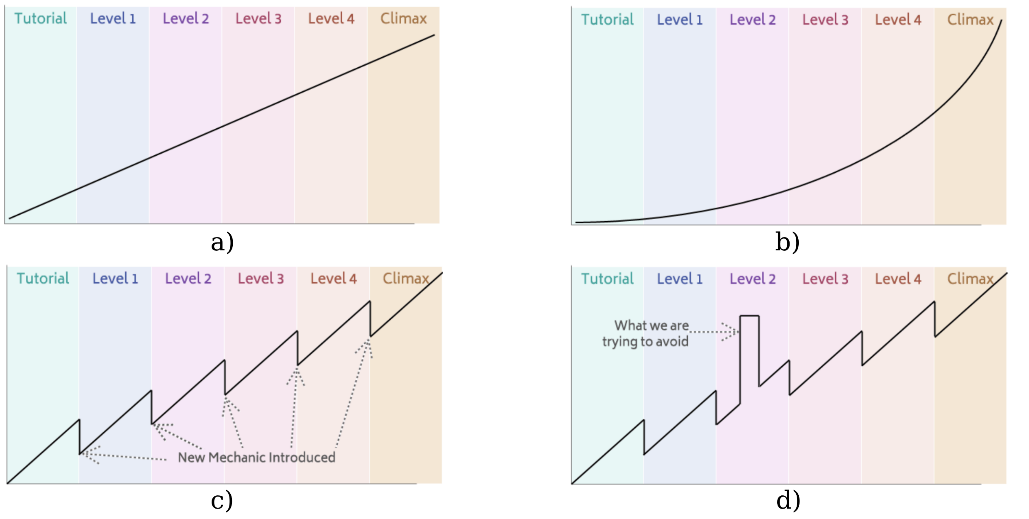
\includegraphics[width=4.58721in,height=2.3558in]{MyThesisImages/media/image68.png}
    \caption{Difficulty curve examples a) Steady increase b) Easy to learn hard to master c) Teaching new mechanics d) Sudden difficulty spike, bad design. Source:\cite{strachan_2018} }
\end{figure}


Some more sophisticated games, include complex systems that dynamically
adjust the difficulty levels in real time, by taking into account
numerous variables. Those systems can personalize the gameplay
experience based on each individual\textquotesingle s skill level to
make the game enjoyable to first time players to skilled veterans.

Valve\textquotesingle s Left 4 Dead games, employ a system called The
Director\cite{Director} "that features a dynamic system for game dramatics,
pacing, and difficulty." Instead of predetermined scenarios "the
Director places enemies in varying positions and numbers based upon each
player\textquotesingle s current situation, status, skill, and location,
creating a new experience for each play-through. The Director also
creates mood and tension with emotional cues, such as visual effects,
dynamic music, and character communication."

\begin{figure}[H]
	\centering
    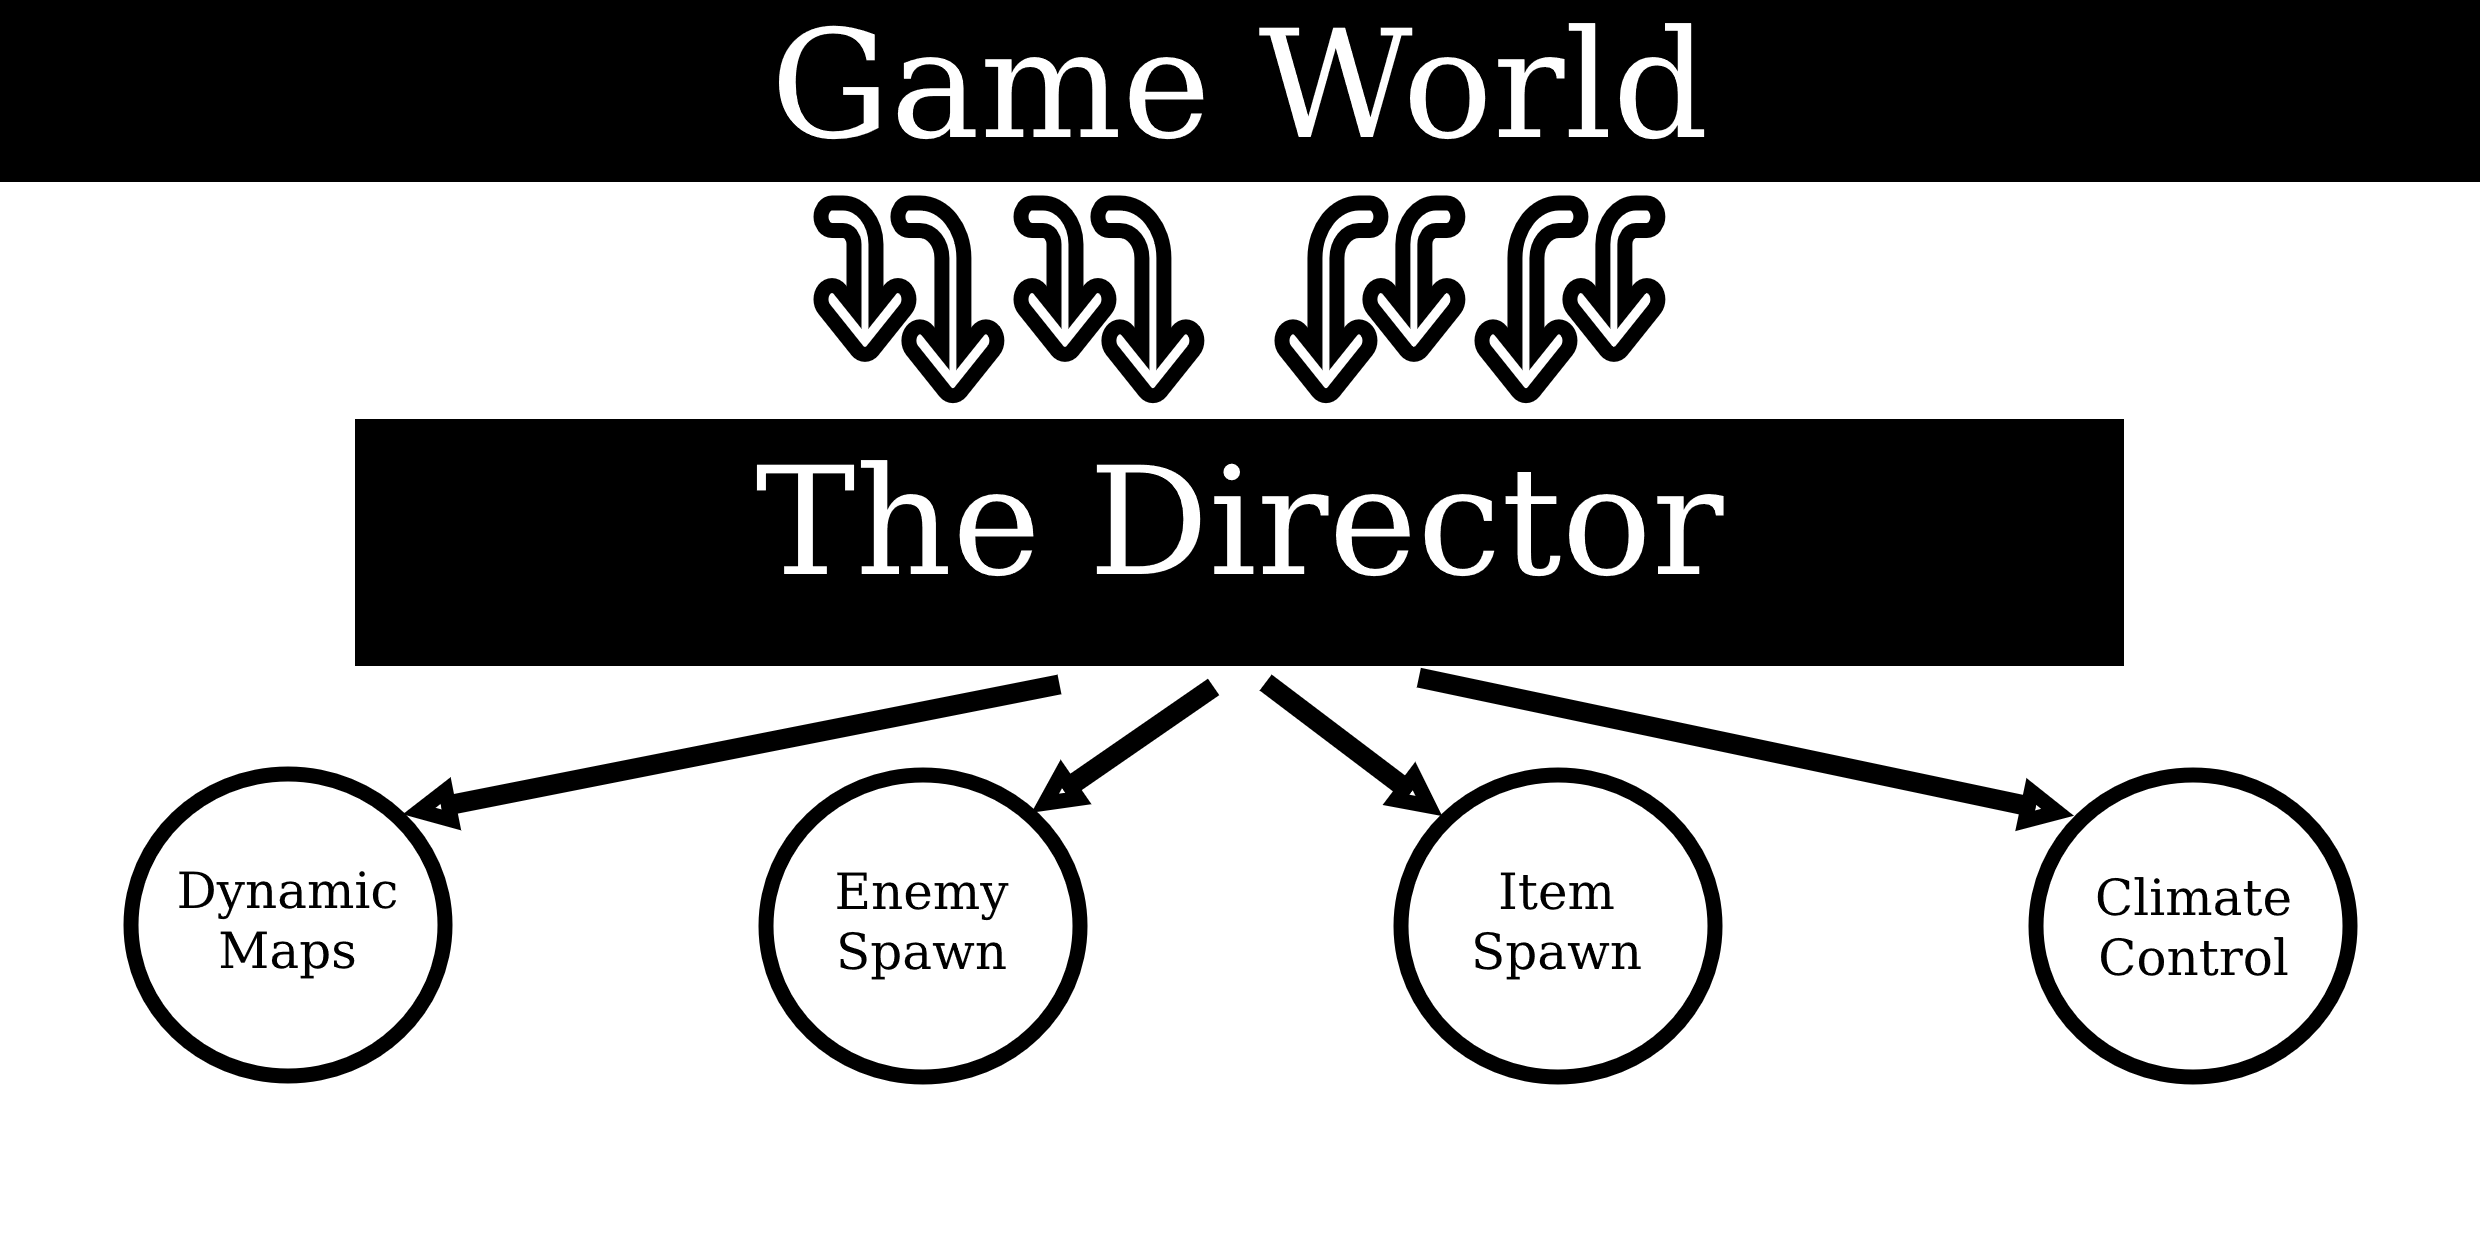
\includegraphics[width=5.09622in,height=2.25194in]{MyThesisImages/media/image69.png}
    \caption{ Overview of the Left 4 Dead 2 director's influence in the game.}
\end{figure}



The games\textquotesingle{} task is to control the pacing and make the
player feel satisfied when overcoming challenges while at the same time
not overwhelming him.

Huge outliers are games with absolutely non-existent gameplay by design.
Often called experiences or walking simulations that are games designed
just to offer a visual journey in awe inspiring environments.

Gameplay along with the World make a great part of the
game\textquotesingle s experience. Managing to combine a beautiful alive
world with an intuitive gameplay can elevate the
players\textquotesingle{} immersion and make them feel like a part of
the virtual world.


\subsection{(Section 3.3.b) Technical Components}

Every game can be dissected down to two individual parts, the Assets and the Logic. The word "Asset" is a broad them referring to a multitude of things that constitute the videogame world, and "Logic" is the underline code that creates a complex network of connections between the Assets.


\paragraph{Assets}

As previously discussed, a lot of different things can be a game asset,
we can classify them as:

\begin{itemize}
\item
  Objects
\item
  Sounds
\item
  Visual effects
\end{itemize}


\subparagraph{OBJECTS\\\\} 

 Objects are the characters, buildings, weapons, props, and every item
the player may or may not be able to interact with.

Every object is comprised of geometry, materials and collision, some
objects can also have animations that make them move in some kind of
way. Depending on the type of game, an object can be 2D or 3D, another
approach is to use 3D but from a locked 2D camera perspective, that
method is called 2.5D. The focus of this section will be on 3D game
development with brief mentions to the 2D counterpart techniques.

\begin{enumerate}
\def\labelenumi{\arabic{enumi}.}
\item
  \textbf{Geometry}
\end{enumerate}

An Object\textquotesingle s geometry or often called "Mesh" is defined
as collection of 3 dimensional vectors that form triangles which
combined create a visualization of a shape in the game world.

In early 3D games, objects were limited to a small number of triangles,
but as computational power increased so did the triangle count.

\begin{itemize}
\item
  1996: Crash bandicoot\textquotesingle s model was 512 polygons,
  roughly 1024 triangles
\item
  2004: Half life\textquotesingle s 2 Alyx was 8000 triangles
\item
  2011: Elder Scrolls V: Skyrim player character with full armor and
  weapon, estimated around 30.000 triangles.
\item
  2024: Characters are about 100-200 thousand triangles.
\end{itemize}

\begin{figure}[H]
	\centering
    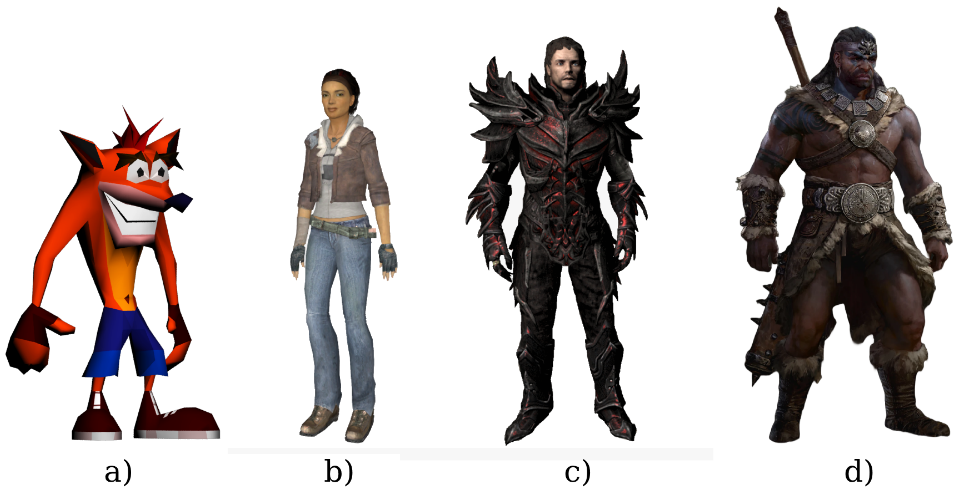
\includegraphics[width=4.34792in,height=2.21119in]{MyThesisImages/media/image70.png}
    \caption{ a) Crash Bandicoot b) Half-life 2 - Alyx c) Skyrim Daedric Armor d) Diablo IV Barbarian.}
\end{figure}

In modern video games employ a variety of technics to reduce the
hardware strain from geometry. A common practice is Level of Detail or
more commonly referred as LODs.

\begin{figure}[H]
	\centering
    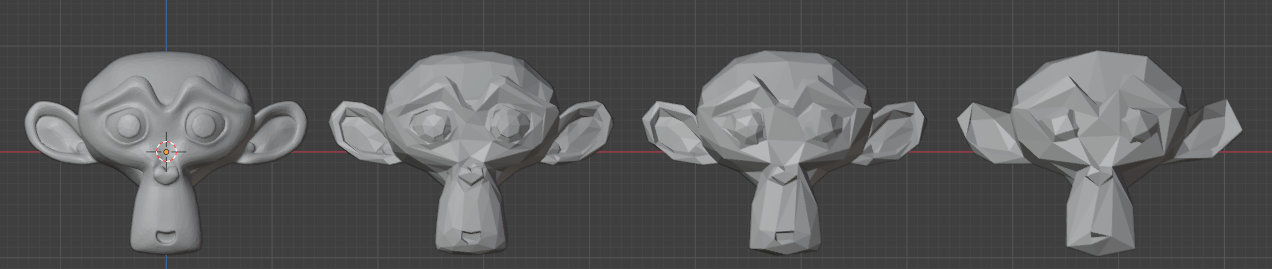
\includegraphics[width=6.25764in,height=1.32569in]{MyThesisImages/media/image71.png}
    \caption{ Example of LODs. Left-most is closest to camera Right-most the furthest away.}
\end{figure}

LODs are a variation of the same object's geometry but with a lower
triangle count which changes depending on the object\textquotesingle s
distance from the player. It allows for rendering of detailed models
close to the camera while far away objects become low resolution for
performance\textquotesingle s shake.

\begin{enumerate}
\def\labelenumi{\arabic{enumi}.}
\setcounter{enumi}{1}
\item
  \textbf{Materials}
\end{enumerate}

A material is a combination of different texture maps that make up the
surface rendered on the geometry.

Modern videogames use the Physical Based Rendering, PBR for short,
material pipeline that includes multiple variables that control the
rendering of the surface.


  \begin{multicols}{2}
    \begin{itemize}
    \item Color 
    \item Normal
    \item roughness 
    \item metallic
    \item specular
    \item ambient occlusion
    \item emissive
    \item opacity
    
    \end{itemize}
    \end{multicols}

\begin{figure}[H]
	\centering
    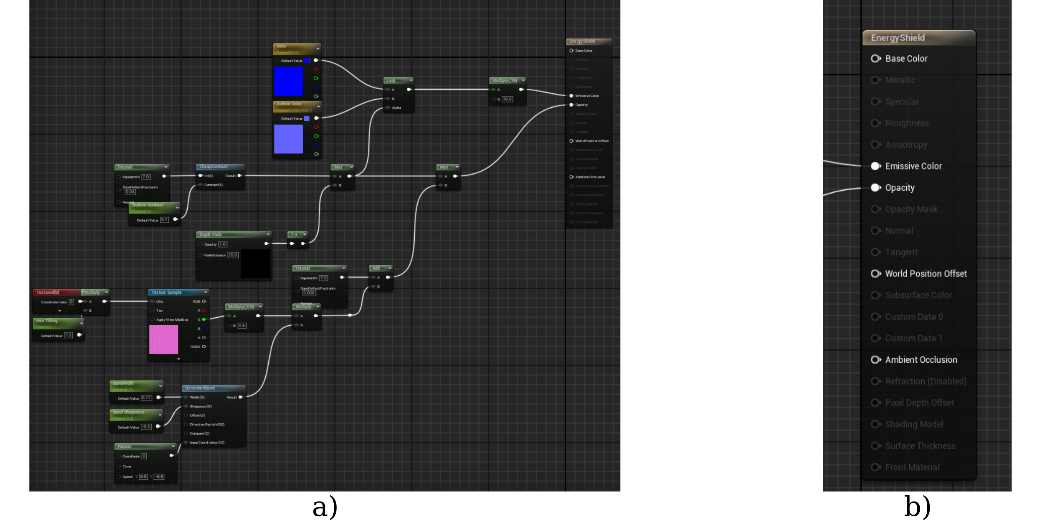
\includegraphics[width=4.725in,height=2.38452in]{MyThesisImages/media/image72.png}
    \caption{ a) Animated Materia example from unreal engine 5. b) List of all supported maps used in unreal engine's PBR workflow. In this case (Opaque) only the supported ones are enabled for use.}
\end{figure}


Those are the most commonly used in the game development process and
each one is represented by a specific image map that has a significant
effect on the final material.

Although not necessary to use the PBR pipeline, only a single texture
map can be the material, the surface rendering quality is far greater
than the flat texture on the geometry.

Despite the evolution of 3D graphics, development of 2D games have not
stopped. The technical approach is similar but restricted due to the 2D
nature of the game. The object geometry is confined to square plains
with one or more materials rendered on them.

\begin{enumerate}
\def\labelenumi{\arabic{enumi}.}
\setcounter{enumi}{2}
\item
  \textbf{Collision}
\end{enumerate}

In game development in order to make different objects interact with
each other or the player, a system must be in place to detect when one
geometry is intersecting another or it is within a very small distance
tolerance, that system is called collision detection and is a very
useful technic applied in various parts of the game.

Making objects rigid and not having them just be a 3d projection of an
image is important. A player character should be able to stand on top of
a surface and not fall though it, so every object along with the
geometry and the materials, it has a collision field.

There are two types of collision:

\begin{itemize}
\item
  Simple collision can be an assortment of basic shapes like boxes or
  spheres that wrap around an object.
\item
  Complex collisions can be either the objects geometry itself or more
  commonly an LOD of the same mesh.
\end{itemize}

\begin{figure}[H]
	\centering
    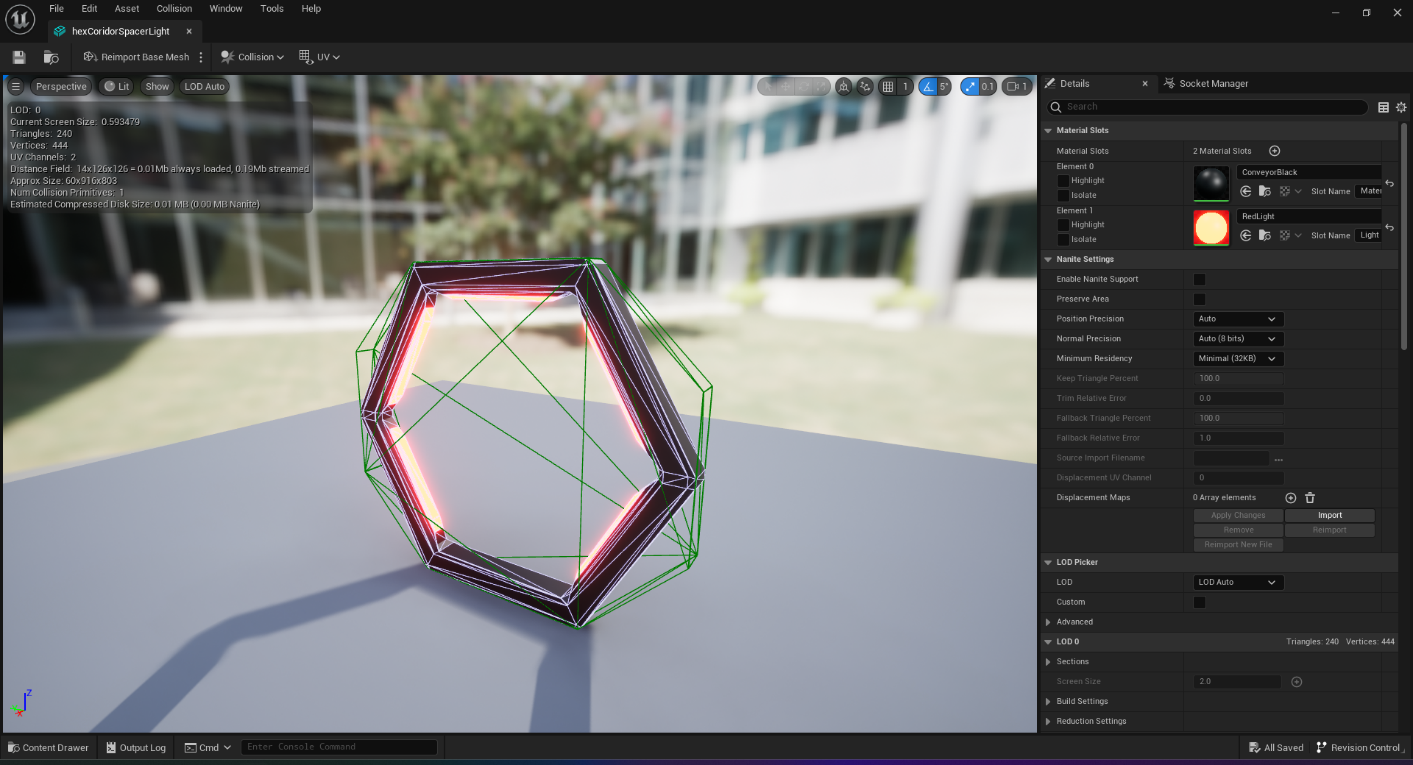
\includegraphics[width=2.53333in,height=1.95697in]{MyThesisImages/media/image73.png}
    \caption{  Collision example from unreal engine 5. The GREEN lines
represent the simple and the WHITE lines the complex collision.}
\end{figure}

Collisions give objects the ability to interact with other
objects' collision and creating a perception of
rigidity inside the game world, but more complex collisions have a
performance impact on the game, it is advised to use simple collisions
in the majority of circumstances and complex collisions must be reserved
for special cases.


\subparagraph{SOUND\\\\}

An essential part of every game, sounds give life to the game and boost the immersion of the player inside the virtual world.

Michael Cullen of the University of California, offers a break down in
Sound Design featured in games\cite{cullen_basics} and can be categorized as:

"  DX = Dialogue - any verbal speech in the game.

MX = Music - any non-diegetic music.

SFX = Sound Effects (Hard Effects) - any sound from a real-life
object.

 FOL = Foley - any sound effect that the player makes.

 BG = Backgrounds (ambience) - noise from the environment."
A lot of players do not find it appealing to read long story scripts or
dialogues while having to stop their gameplay. DX offers the players the
ability to continue playing while a narrator tells the story and hear
the characters talking with each other.

Game music and ambient sounds set the mood and tone of the scene, adding
tension and suspense to the gameplay.

SFX are sounds recorded from real life and imbedded inside game objects
to make the player's interactions have audio feedback
along with the visual, greatly increasing the feeling of immersion.

Foley sounds are similar to SFX, they the include character footsteps,
breathing, cloths rubbing while walking or running and give an added
feel of realism to the game.

Modern games implement sound localization technologies, also known as
spatial sound or 3D sound, used with SFX and DX to simulate the sense of
space inside a 3D game world.

Sound is not only for aesthetic purposes but has a role in gameplay too
as they can be used to enhance and assist various game mechanics.

Spatial sounds give the world a lot more realism and should not be left
out of any game. The most basic example is pinpointing enemy location
based on where the gun sound is coming from instead of using visual
indicators.


\subparagraph{VISUAL EFFECTS\\\\}

Visual effects referred commonly as VFX were part of mainstream
industries like film and TV, but as computing power increased, games
started adopting it immediately as is the next level of realism and
creating life in a digital environment. The difficulty of implementing
VFX systems inside games is greatly impacted by the need of real time
rendering.

Films have the advantage of being prerecorded and can be rendered as
long as needed in huge distributed systems to get the desired quality,
games on the other hand are played and interacted with in real time,
that poses a huge trade-off between hardware limitation and desired VFX
quality.

Developers try make the most efficient used of the screen space and find
workarounds to minimize the trade-off in creative ways by:

\begin{itemize}
\item
  limiting the use of VFX only where the player can see.
\item
  using a technic similar to object LODs to set the appropriate quality
  depending on the VFX.
\end{itemize}

Game VFX Categories:

\begin{itemize}
\item
  Lighting
\item
  reflections
\item
  animation
\item
  particle systems
\end{itemize}

\begin{enumerate}
\def\labelenumi{\arabic{enumi}.}
\item
  \textbf{Lighting}
\end{enumerate}

There are 3 types of lighting used in the game development process.

\begin{enumerate}
\def\labelenumi{\arabic{enumi}.}
\item
  Static lighting rendered during the development process on top of the
  affected surfaces and can not change after the fact, also known as
  Baked lighting.
\item
  Dynamic lighting rendered in real time by calculating the light source
  position in space and lighting the surfaces dynamically inside a
  specific area of effect.
\item
  Ray Tracing lighting "is a rendering technique that can realistically
  simulate the lighting of a scene and its objects by rendering
  physically accurate result".\cite{nvidia_2018_ray}
\end{enumerate}

Most would immediately choose the use of Ray Tracing as it delivers the
most realistic result possible, but taking in consideration the
performance costs the player base will dramatically be reduced due to
the minimum hardware requirements, it is a new technology used on the
best and most realistic games.

Baked lighting has no performance cost at run-time but has the huge
limitation of not being able to effect moving objects or static objects
that are added during gameplay.

Dynamic lighting can affect moving objects and can have a light source
that moves around in space, it is the most realistic approach but also
has a high-performance cost during run-time.

Both have their advantages and disadvantages, the optimal solution is a
per case mixture of both technics, the choice is in the hands of
developers to make based on the desired result.

\begin{enumerate}
\def\labelenumi{\arabic{enumi}.}
\setcounter{enumi}{1}
\item
  \textbf{Reflections}
\end{enumerate}

Reflections are very similar to lighting as they are split between
static/baked and dynamic/real-time reflections but both categories
employ more than one technic for rendering.

Reflection Technics

\begin{itemize}
\item
  Planar Reflections
\item
  Screen Space Reflections
\item
  Cube Maps
\item
  Ray Tracing Reflections
\end{itemize}

All technics can be used baked or real-time depending on the developer's
decision, but a combination of technics is advised for achieving optimal
results.

\begin{enumerate}
\def\labelenumi{\alph{enumi})}
\item
  Planar reflections
\end{enumerate}

Using a virtual camera to capture the reflections and render them in the
scene. Offers good quality reflections but it is a very resource
demanding approach because a separate render pass is required.

\begin{enumerate}
\def\labelenumi{\alph{enumi})}
\setcounter{enumi}{1}
\item
  Screen Space Reflections
\end{enumerate}

The most efficient and widely used type of reflection generation technic
uses the already rendered frame to calculate the reflections but comes
with a significant limitation, it can not render what the camera does
not see, resulting in many artifacts and medium quality reflections when
combined with harsh camera angles and rough surfaces.

It is most often used on water or floor surfaces and not as an
independent system for all reflection needs of the game.

\begin{enumerate}
\def\labelenumi{\alph{enumi})}
\setcounter{enumi}{2}
\item
  Cube Maps
\end{enumerate}

Introduced by Nvidia in 1999 but still being a relevant technic for
reflective but not mirror surfaces. Cube mapping uses an invisible
square and it's 6 facets to capture the reflections from
the surrounding scene and create 6 texture maps to stich and wrap around
the object.

\begin{enumerate}
\def\labelenumi{\alph{enumi})}
\setcounter{enumi}{3}
\item
  Ray tracing Reflections
\end{enumerate}

Ray tracing is not used only for lights, by bouncing the rays on top of
each object it generates physically accurate reflections \cite{nvidia_2018_ray}. The
resulting render is impressive but similar to Ray traced lighting it is
the most resource expensive technic.

\begin{enumerate}
\def\labelenumi{\arabic{enumi}.}
\setcounter{enumi}{2}
\item
  \textbf{Animation}
\end{enumerate}

Having animations is the first and most important step for giving it
life to every game. Depending on the type of game animations can be
separated as 2D and 3D.

\begin{enumerate}
\def\labelenumi{\alph{enumi})}
\item
  2D Animation
\end{enumerate}

Making games in 2D is very similar to making traditional 2D cartoons.
Hand drawn or digitally created images are played in quick succession in
order to give players the perception of moving objects.

Despite being based on the same core technic game animations have a very
significant difference, the scene is not drawn as a single picture
frame, each object is animated independently and composited on the
scene.

\begin{enumerate}
\def\labelenumi{\alph{enumi})}
\setcounter{enumi}{1}
\item
  3D Animation
\end{enumerate}

Animating 3D objects is not as easy as drawing the next 2D animation
frame, is requires the use of a special technic known as a "Rig". Every
3D object must be "rigged" before being animated. The role of a rig is
to influence the coordinates of the object's vertices in
space. On simple objects rigging is the placing of one or more hinging
point but on more complex objects like humanoid characters a more
advanced rig is required that plays the role of the bones and
it's often called "Armature" or "Skeleton". Depending on
the desired animation fidelity the skeleton's bone count
changes.
\begin{figure}[H]
	\centering
    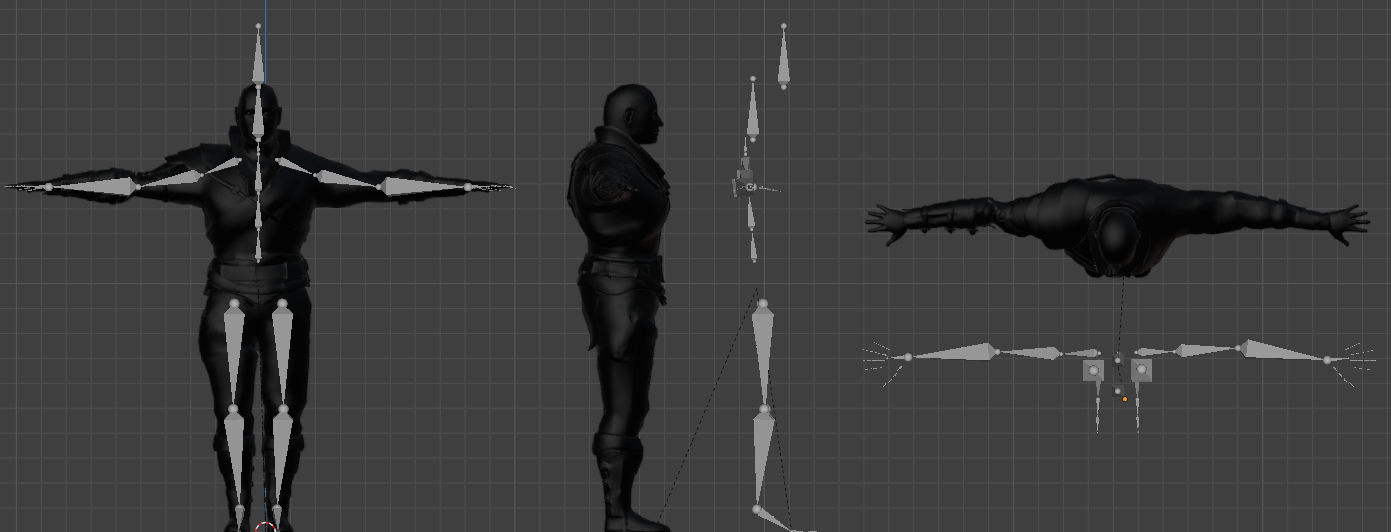
\includegraphics[width=5.85606in,height=2.24013in]{MyThesisImages/media/image74.png}
    \caption{Armature and mesh(displaced) from front, side and top view.}
\end{figure}


The animators create key frames or poses by manipulating the bones.
Interpolating between poses creates the final animation. Animations can
have 2 or more key frames depending on their complexity. Mathematical 3D
vector coordinate interpolation is not enough to provide smooth
animations, increasing or decreasing the number of key frames will
dictate the fluidity of each animation.

Creating simple animations is not a hard task on its own, making physics
accurate complex animation that blend seamlessly with each other is
another matter. Thankfully there are tools on the market that assist
with the physics simulation part of the animating procedure, enabling
developers to create realistic results with less work, thus increasing
individual productivity, immensely important in small development teams.

\begin{enumerate}
\def\labelenumi{\arabic{enumi}.}
\setcounter{enumi}{3}
\item
  \textbf{Particle Systems}
\end{enumerate}

Particle systems are a core aspect of visual effects, they are a vector
field consisting of small images or 3D objects that act independently
based on forces acting upon them.

They are used for "fuzzy" effects like fire, smoke, explosions and other
similar vfx. The number of particles used will often dictate the quality
and realism of the effect, more particles mean more quality but their
independent nature links the computational cost to the particle count
making them a very resource expensive system.

The main component of a particle system is called particle emitters and
is responsible for the way the particles are emitted from the source and
keeping track of each individual particles variables. A particle system
can have multiple emitters active at the same time or one after another,
in order to achieve the desired effect.

Most important particle variables

\begin{itemize}
\item
  color
\item
  size
\item
  velocity
\item
  rotation
\end{itemize}

Every particle has a huge number of variables, some of them remain
static and some of them follow curves in order to change their value
during every particle's life span.

\textbf{List of emitter types}

"Sprite Emitters - These are the most basic types of emitters and the
most frequently used. Particles are emitted as polygonal sprites
(2-polygon cards) which always face the camera. Useful for smoke, fire,
and a wide variety of other effects.

AnimTrail Data - Used to create trails from the sockets of animated
skeletons.

Beam Data - Used to create beams such as lasers, streaks of lightning,
and similar effects.

GPU Sprites - These are special types of particles in which the bulk of
runtime calculation is passed off to the GPU. This boosts the number of
possible particles from the several thousand possible with CPU particles
to several hundred thousand, depending on the type of GPU in the target
system.

Mesh Data - Instead of emitting a series of sprites, this type of
emitter will instead emit polygonal meshes. Great for rockslides,
debris, and similar effects.

Ribbon Data - This produces a string of particles that are attached end
to end to form a ribbon which trails behind a moving emitter."\cite{particles_ue}

\textbf{Particle system Optimization}

As discussed previously, particle systems are a very resource expensive
technic and as a result there was a need for optimizing their
performance.

Particle System Level of Detail is the most common way to enable
developers to minimize that cost by reducing texture quality or even
disabling entire emitters when the camera is at a far enough distance
from the system that the player would not notice a difference.


\paragraph{Logic\\\\}

In the previews segment we list and analyzed in depth all the components
that constitute a video game, but those components themselves can not
make a video game. As chess pieces do not make chess what it is,
objects, vfx and animations do not make a video game, they are just the means with which the games rules and gameplay are enacted by the
players.

In the realm of video game development, the rules of the game are the
logic imparted within the other components, interconnecting them with
each other and creating a complex web of in-game system interactions.
Every game is an event driven interactive experience that each player
delves into and with his actions effects those events inside the virtual world.\\

\textbf{Types of Events}

\begin{enumerate}
\def\labelenumi{\arabic{enumi}.}
\item
  {Button press Events.}
\end{enumerate}

The simplest type of in-game interaction. When a player presses a
keyboard or a controller button an in-game event is triggered resulting
on a predefined scenario to be executed.

Common button press events:

\begin{itemize}
\item
  Character animations like walking, running, jumping.
\item
  Weapons firing attacks
\item
  Opening menus
\item
  User interface mouse clicks
\end{itemize}

\begin{enumerate}
\def\labelenumi{\arabic{enumi}.}
\setcounter{enumi}{1}
\item
  {Collision Based Events}
\end{enumerate}

Collision Detection in videogames is not only used for rigid bodies,
another crucial implementation of collision is also event triggering.

Primitive shapes like boxes and spheres are employed to detect when
another object's geometry is overlapping them in order
to trigger a specific scenario.

Those shapes are called collision boxes and remain invisible to the
player but they play an important role in the
developer's part.

Common Collision Based Events

\begin{itemize}
\item
  Proximity Opening Doors
\item
  Playing a Sound
\item
  Assuring proper player character position
\item
  Player in range to allow specific action.
\end{itemize}

\begin{enumerate}
\def\labelenumi{\arabic{enumi}.}
\setcounter{enumi}{2}
\item
  {System Events}
\end{enumerate}

Many games implement complex systems that do not require direct player
action to initiate, they exist in the game so the player may interact
with them.

Including mechanics such as simulating a damage system, an enemy AI
system, an in-game economy, or a reputation system. Their role is
keeping track of a vast array of game variables, listening to changes
that may happen during gameplay and triggering events depending on
certain conditions the developers set.\\

\textbf{Summary}

The logic in every game, gives life to otherwise lifeless objects and
enables player interaction inside the world created by the game makers.
Game Logic can be complex or simple depending on the
game's intentions, but a more complex game does not
necessarily mean a better game and a simple game does not mean a boring
game. Creating interesting and unique gameplay is not a matter of
complexity, but rather a matter of creativity and understanding of the
player-base desires.

The majority of players are not playing a game to become the best and
making them feel that is necessary to "study" the game mechanics in
order to enjoy it, will deter them from playing. Implementing intuitive
systems and gradually introducing the complex ones to the players is key
in developing a successful game.


\section{(Sub-chapter 3.4) Chapter Conclusions}

In this chapter it was attempted to define the concept of video games in
a philosophical and sociological way by their impact to the world and
offer a comprehensive analysis on the theoretical and technical parts of
the process of making a video game as will as the required specialized
roles that contribute to the final product from the conception of the
idea to the release of the game.

It is evident that before attempting to tackle the technical aspect of
the process and assume a role in a development team, someone must have a
good understanding of the nature of video games as well as a broad view
of the entire process as each part interlocks with each other to produce
a single coherent game without inconsistencies between the different
parts.

\pagebreak

\chapter{CHAPTER 4 Challenges of Video Game Development and Benefits of Employing AI}


\section{(Sub-chapter 4.1) Challenges Depending on the Scale}

Modern Gaming has become a huge entertainment industry. As games set
higher and higher standards, major titles required the involvement of
more and more people, that lead to the formation of huge publishing
studios comprising of many development teams. Todays AAA titles need
hundreds of skilled people, each one being specialized in one aspect of the process and take multiple years to develop.

Despite the difficulty, individuals did not stop pursuing game
development. With open-source software solutions available and companies
offering free public access to their software in exchange for royalties,
many people joined the development scene individually or in small teams.
Independent studios were born and unrestricted from corporate interests,
they were free to explore innovative and niche ideas.

\subsection{(Section 4.1.a) Large Scale game development}

Large scale game development produces games of great quality, pushes the
technological limits and moves the gaming industry forward, but all that
comes with a lot of challenges that need to be addressed and overcome.

\textbf{{Size}}

In the first years of video game development, one person or teams of a
few people were developing videogames. As videogames moved from a
research field to a small niche part of the entertainment industry,
players as well as developers started demanding for higher quality
games, that inevitably led to the addition of more and more people in
the development teams to help with the growing demand and quality
expectations.

When games hit the mainstream and major corporations started seeing them
as an investment opportunity, they started pouring money expecting good
turnovers. Increasing pressure from investors and from the player base
caused the development studios to exponentially increase their size.

Game development Studio approximate size list:

\begin{itemize}
\item
  Small: 15-50 people
\item
  Medium: 50-100 people
\item
  Large: 100-500 people
\item
  Extra Large: 500+ people
\end{itemize}

\textbf{{Human Resources Management}}

Large scale development regularly faces the problem of employee
management due to the large number of people involved in the game
development process but also because more often than not the studios are
split across multiple locations and countries.

It is very difficult to create a maintain an inter-team communication
system spanning hundreds of people, when at the same time trying to
maximize productivity and have strict production time frames.

\textbf{{Late-Stage Technical difficulties}}

At the later stages of the development process, unexpected technical
difficulties may be presented and delay the release date. Especially in
Massive Multiplayer Online (MMO) games that want to release in multiple
countries, the server solutions that seemed adequate during the testing
process, may prove to be problematic in a larger player influx and
require complete redesign of the game's infrastructure.

Another late-stage challenge is finding pacing problems during the final
larger scale testing process. Players completing the game faster than
expected or having a hard time understanding the mechanics of the game,
thus losing interest. It can prove to be a major step back and create
huge delays.

\textbf{{Art out-sourcing}}

It is not uncommon for development studios to outsource art in order to
focus on the technical aspects of the game and the mechanics, but poor
communication between the two parties can create problems. Realizing
after the fact that the outsourced art is not on par with the quality
requirements after spending huge sums of time and money while creating
the need to outsource again with a different studio or create it
in-house will dramatically delay production and will increase costs.

\textbf{{Huge production times and market pressure}}

It is not uncommon in large scale game development production time to be
in the multiple years ranging approximately between 3 to 7 years
{[}32{]} and in some rare cases even more. During such large development
periods the industry's advancements may be so big that the game ends up
seeming outdated in terms of graphics or mechanics, forcing studios to
try catching up with current trends and technology. Changing game
engines one or multiple times during the development will inevitably
lead to major delays and technical difficulties.

\textbf{{Code Rot}}

Code rot, also known as software rot or bit rot, describes the tendency
of software to fail when it encounters an exceptional condition. If the
design was insufficiently robust and assumptions made during development
become out of date, this may cause it to fail in unexpected ways.

It is common that code written for the game in the prototyping stages
may not be optimized for long time maintenance or account for every
possible scenario and will need to be redesigned in the later stages of
development.

A prime example of code rot was when some early video games tied some of
the games' functions to the CPU clock speed. Later when users upgraded
to a faster system the games ended up being unplayable due to bad
foresight and design decisions.\cite{salemi_1992_slowing}

\textbf{{Uncertainty}}

The game designing process is a very difficult task and always includes
a level of uncertainty as it tries to appeal to many peoples' subjective
opinion on what a good video game is.

During the development of a game, huge chunks of the game may be
discarded or redesigned from scratch. Revising the games' vision midway
through the production and radically changing the art style of the game
or redesigning the mechanics of the game to fit better with the overall
feeling and storyline, will cause a major setback in both time and money
for the studio.

\textbf{{Maintenance}}

Most prevalent in online games, maintenance is a core aspect of a game's
lifecycle. Balancing, bug fixing, updating the outdated and releasing
new content is essential in prolonging a video game's life and maintain
relevance for a long period time.

It is very costly to even maintain a game in it's released state, keep
adding content is even harder. Many companies try to utilize
micro-transaction systems for in-game purchases in order to keep
financing the post-release support of the game. These micro-transactions
can be for purely cosmetic, or they can give an in-game advantage by
affecting the player's performance, the first do not bother the player
base but the latter are considered as underhanded pay-to-win methods.
Companies who used those pay-to-win approaches are heavily criticized
for being greedy and for using underhanded paywalls.


\subsection{(Section 4.1.b) Small Scale game}

When a small team tries to tackle an enormous challenge, such as
developing a game, each individual will be assigned with multiple roles
and the workload as well as the responsibilities are increased
exponentially. Often "projects have ambitious goals that may or may not
be underestimated during the design phase, causing delays in trying to
reach those goals to a high degree. They get stuck in development for an
extended period of time, never make it to production and are gradually
abandoned by the people involved"\cite{juego}. This is called
"Development hell" and it is very common among inexperienced independent
teams.

According to Juego Studio \cite{juego}, a software and game development
company based in India and operating internationally, this is a list of
challenges that make projects fall in Development Hell:

\begin{itemize}
\item
  Poor project planning
\item
  Financial challenges
\item
  Unforeseen technical issues
\item
  Licensing and legal issues
\item
  Change in management.
\item
  Technology changes
\item
  Unrealistic deadlines and overly ambitious project
\item
  Internal conflict
\end{itemize}

Careful planning in the early stages of development, depending on the
team\textquotesingle s capabilities but also resource restrictions such
as budget and setting an appropriate shipping deadline, are essential to
avoid falling in Development Hell.

\
\section{(Sub-chapter 4.2) Benefits of Employing AI in Game Development}

The videogame industry depends on the cooperation of many specialized
experts for every aspect and component that constitutes a video game,
making it very resource expensive in both time and money. The employment
of AI technology is a natural step forward in the quickly expanding
field of video game development.

Artificial intelligence can be used to assist in the development of
video games by analyzing players' data mined from playing games as well
as player reviews, making it possible to identify trends and patterns in
the player base's behavior. Such analysis would be impossible without
the use of data mining and machine learning algorithms that provide the
developers with valuable data and enable them to create the best games
possible.

A new leap in AI technology is Generative Artificial Intelligence that
is capable of language and media generation by recognizing patterns of
the data provided in the training dataset and can generate:
\begin{multicols}{2}
\begin{itemize}
  \item Text     
  \item Code 
  \item Image	
  \item 3D geometry
  \item Video 
  \item Sound 
  
  \end{itemize}
\end{multicols}
There is a plethora of trained Generative AI tools on the web, most of
them are utilizing a text or tag-based input system in order to generate
media using keywords and descriptions the users provide.


\subsection{(Section 4.2.a) Prototyping}

Generative AI can prove a very useful tool in the prototyping phase of
the development, enabling designers to visualize their ideas while
brainstorming, shift between different art styles, character, and level
designs to see what will suit their vision of the game.

On the technical side of things generative AI can provide crud and
simple models and textures so the developers have an initial start point
that can be later refined as necessary.

Fast prototyping can impact the pace of the production process and give
a huge head start to the developers.


\subsection{(Section 4.2.b) Productivity}

As generative AI continues to evolve, it can be used to increase
productivity during the development process.

Artists don't have to start painting textures from scratch or design the
3D models vertex by vertex, AI can give them a head start and let them
refine and build upon a generated base.

Make story telling easy by writing the main points of a script and let
AI fill the not so important details or let it create stories branching
away from the main plot in order to fill the game with more content
without interfering with the basic premise of the game.

Composing songs and sound effects can become easier for the developers
as AI can give them original ideas and stop them from getting stuck
during the creation of new and innovative music.

Having AI do the repetitive and mundane jobs during the early stages of
development can dramatically increase productivity. AI voice overs and
narration of the game can help developers get a feel of the final
product before investing the time and money hiring voice actors.

Level and environment composition with topology and topography-based AI
algorithms can reduce the workload of designers immensely, as they only
need to go and refine the levels after the AI has done the repetitive
job of placing models one by one to populate the scene.

\subsection{(Section 4.2.c) Individual or Small teams}

Individual and small teams must shoulder the burden of all the required
roles necessary for game development. The quality of the generated
content provided by the latest AI can be enough so it can be assigned
and take over the responsibilities of a specific role.

By splitting the workload and assigning multiple AIs for their
respective tasks, developers can make it easier for them to pursue game
development and not get overwhelmed from the knowledge requirements, by
reducing the repetitive tasks or filling in for a missing spot of a
person with the appropriate specialized knowledge of a field.

\subsection{(Section 4.2.d) Realism, Immersion and Replay-ability}

A huge field of study in AI used for game development are
implementations of behavioral AI models that enhance the process of
interaction within game characters humanoid or not and bring the virtual
game world closer to a more realistic representation.

Immersion can be elevated as conversations and interactions will not
just be a set of questions and answers read from a script and repeated
the same way every time the game is replayed, but they will be dynamic,
guided by the script but changing every time thus producing and infinite
amount interactions and encourage more replay-ability.

\subsection{(Section 4.2.e) Post-Release Maintenance}

Online games, besides the development process, require constant
post-release maintenance and balancing. It is one of the most important
and difficult aspects of online games especially if they are in a
competitive e-sport scene. That is the reason why small developer
studios do not even try to get into that part of the video game market
due to the financial cost but most importantly the cost to sacrifice a
team member from development to maintenance.

There are discussions by many video game developers to implement an
artificial intelligence system to assume the role of the game manager
and oversee a single game or a platform including multiple games in real
time as the players interact with them. It may have the ability to
control some parameters to steer the player behavior in a certain
predefined preferred way or just log and make reports for the game
developers to address.

It would be a major asset that would enable more games and ecosystems of
games to be managed by a single AI entity while freeing the hands of the
developers and letting them focus on producing new content and games.

\subsection{(Sub-chapter 4.3) Negative Effects of AI}

Even with all its benefits AI technology does come with a fair share of negative effects as well.
In this section we will discuss three of the most important ones in order to showcase that 
nothing comes with only benefits, there are always some drawbacks in some way or another.

\subsection{(Section 4.3.a)Reduction of jobs}

With the constant evolution and improvement of AI based solutions,
many mundane and repetitive tasks where outsourced to AI as it was 
very cost effective and didn't require training to do the job like a
person would. 
That lead to a reduction of job positions especially in the entry-junior 
developer level. Making it harder for new people to get in the industry not 
only for game development but in general software development.

As a result as aspiring beginners have to upskill fast on their own before 
being able to have all the requirements for a junior-mid developer position.
  
  
\subsection{(Section 4.3.b)Sentiment of uncertainty}

After seeing the capabilities demonstrated by the state of the art AIs,
a sentiment of uncertainty was cultivated even to the most seasoned of developers.
Many fear that AI will take over most of the tasks, which will lead to many fields of
development being obsolete in the future. Rushing to specialize in a field which they 
believe to be safe at least for the foreseeable future as well as deterring everyone who
might show interest in any of the fields they believe to be vulnerable to AI overtaking.


\subsection{(Section 4.3.c) Over-reliance on AI}

An over-reliance on AI happens when users believe the AI without considering if its suggestions
are correct or not. Most people have an idealistic view of AI and are not able to determine
the appropriate levels of trust.
An AI tool, even if its capable of delivering impressive results, it should not be trusted
completely. Regardless of its complexity, it remains an algorithmic procedure which still 
lacks qualitative capabilities compared to the human mind. The outputs generated by AI technology
should always be scrutinized by at least one human expert and cross-referenced in order to verify 
the correctness of the output.


\section{(Sub-chapter 4.4) Chapter Conclusions}

This chapter is divided in two parts the first was focused on an
in-depth analysis of the challenges faced in modern video game
development during the development process and after the release of the
game in both small and large-scale scenarios. It showed that making a
video game is a very hard endeavor and without a doubt many challenges
will need to be faced until its completion. In the second part there was
a discussion on how utilizing artificial intelligence can improve the
game development process in multiple aspects. By automating parts and
even eliminating entire processes will make game development more
approachable and financially viable for small or individual teams.
Lastly, some of the negatives effects that come with the rise of AI 
technology were discussed as well for the purpose of eliminating any
misconception of AI having only positive impact on the development scene.

\pagebreak

\chapter{CHAPTER 5 Software used in Game Development and Replacement AI tools}


\section{(Sub-chapter 5.1) Software}

\subsection{(Section 5.1.a) Modeler}

Started as Computer Aided Design, CAD, software for digital recreation
of the real world in architecture, engineering, and construction
industries but developed into a complete 3D Model designing suit that
expanded it\textquotesingle s use in film and game industries. A modeler
uses a collection of interconnected points representing various shapes
such as triangles and polygons in 3D space, in order to create a digital
3d model reproduction of a physical object inside a virtual environment.

Every 3D model is comprised of

\begin{itemize}
\item
  Vertices - points in space represented by a (x, y, z) vector
  coordinates.
\item
  Edges - the lines connecting different Vertices.
\item
  Faces - polygons created when a vertex group is closed.
\end{itemize}

Faces can be further analyzed depending on how many vertices create by

\begin{itemize}
\item
  Triangle or tris =3 vertices
\item
  Quad= 4 vertices
\end{itemize}

Even though quads are used in the modelling process, in practice every
3d model is saved as a collection of triangles and every quad is
converted internally to triangles, because a polygon that has more than
3 vertices is not deterministic.

A modeler is capable of creating and editing an immense number of
Vertices, Edges and Faces in order to create models with great fidelity.

Brief timeline of important 3D CAD software

\begin{multicols}{2}
  \begin{itemize}
    \item 	1960 Sketchpad 
    \item   1964 DAC-1
    \item	  1971 ADAM
    \item	  1982 AutoCAD
    \item	  1988 Cobalt	
    \item   1990 Cinema 4D
    \item	  1994 Blender
    \item	  1995 SolidWorks
    \item	  1996 3Ds Max
    \item 	1996 Houdini FX
    
  \end{itemize}
\end{multicols}

All 3d modelling software developed in the 1990s are prevalent and still
industry standard to this day, as they keep evolving to match the
technology advancements.


\subsection{(Section 5.1.b) Painter}

After creating the 3d models the textures that will become the PBR
material need to be painted on top of the geometry. Almost all modelers
come bundled with a simple painter or an independent painting software
with more specialized functionality can be used, depending on the needs
of the artist.

Some of the industry standard painters are:
\begin{multicols}{3}
  
\begin{itemize}
\item
  \begin{quote}
  Substance painter
  \end{quote}
\item
  \begin{quote}
  ZBrush
  \end{quote}
\item
  \begin{quote}
  Quixel Mixer
  \end{quote}
\item
  \begin{quote}
  Blender
  \end{quote}
\item
  \begin{quote}
  ArmorPaint
  \end{quote}
\end{itemize}
\end{multicols}

\subsection{(Section 5.1.c) Audio Software}

To record or edit the sound that will be used in the game, an assortment
of software is needed for recording and editing sound effects, narration
and mixing music.

Audio software for used in game development falls in two categories:

\begin{enumerate}
\def\labelenumi{\arabic{enumi}.}
\item
  \begin{quote}
  Game Audio Tools
  \end{quote}
\item
  \begin{quote}
  Digital Audio Workstations
  \end{quote}
\end{enumerate}

Game Audio tools, also referred as middleware, are different tools
designed with game development applications in mind. They focus on 2D as
well as 3D audio and also on offering solutions for interactive
scenarios by understand different states of the game and dynamically
parameterizing the sounds being played in real time during gameplay.

They are easily integrated inside the game engine of choice to provide
an easy workflow for non audio expert users.

A list of the most used Game Audio Tools

\begin{itemize}
\item
  \begin{quote}
  Wwise
  \end{quote}
\item
  \begin{quote}
  FMOD
  \end{quote}
\item
  \begin{quote}
  Miles Sound System
  \end{quote}
\item
  \begin{quote}
  Fabric
  \end{quote}
\end{itemize}

Digital Audio Workstations are the more traditional audio editing
software offering a vast array of functionalities to the users.

A list of the most used Digital Audio Workstations

\begin{itemize}
\item
  \begin{quote}
  Adobe Audition
  \end{quote}
\item
  \begin{quote}
  Cubebase
  \end{quote}
\item
  \begin{quote}
  Komplete
  \end{quote}
\item
  \begin{quote}
  Audacity
  \end{quote}
\end{itemize}

\subsection{(Section 5.1.d) Game Engine}

The most important software for developing videogames is a game engine.
It can be described as a framework designed for the development of video
games, used by game developers for creating games in different types of
platforms such as mobile phones, consoles, pc, virtual reality.

A game engine includes a variety of subprograms such as:

\begin{enumerate}
\def\labelenumi{\arabic{enumi}.}
\item
  \begin{quote}
  \textbf{Graphics Renderer} - Responsible for combining geometry and
  materials in order to show the final rendered graphics, 2D or 3D, to
  the player.
  \end{quote}
\item
  \begin{quote}
  \textbf{Object Handler} - Keeping track of all game level instances
  and every object instance inside each level.
  \end{quote}
\item
  \begin{quote}
  \textbf{Material editor} - Combining all imported texture maps and
  handling "material specific code" to create the final rendered PBR
  Material.
  \end{quote}
\item
  \begin{quote}
  \textbf{Animation Handler} - Handling all independent animations and
  interpolating between user input and animation being played on screen.
  \end{quote}
\item
  \begin{quote}
  \textbf{Lighting and reflection} Handler - Calculating lighting and
  reflections either dynamically in real time or static baked during the
  development process.
  \end{quote}
\item
  \begin{quote}
  \textbf{Collision Detection Handler} - Detecting geometry overlaps
  between two or more in game objects.
  \end{quote}
\item
  \begin{quote}
  \textbf{Particle System Handler} - System for creating and rendering
  in game particle system simulations.
  \end{quote}
\item
  \begin{quote}
  \textbf{Audio Handler} - Subsystem for handling all audio being played
  in game.
  \end{quote}
\item
  \begin{quote}
  \textbf{Physics Handler} - Subsystem responsible for calculating and
  simulating physics interactions between game objects.
  \end{quote}
\item
  \begin{quote}
  \textbf{AI Handler} - Subsystem for creating predetermined AI
  behavior scenarios based on real time in game variable changes.
  \end{quote}
\item
  \begin{quote}
  \textbf{Input Handler} - Automatic input handling subsystem for
  keyboard, game controller or other input device.
  \end{quote}
\item
  \begin{quote}
  \textbf{Memory Handler} - Automatic computer memory handling based on
  real time game requirements.
  \end{quote}
\end{enumerate}

Those are the core subsystems that constitute the game engine ecosystem,
but on top of them a lot more can be added to increase functionality in
the form of plug-ins or integrated subsystems included with new versions
of the game engine.

A list of the most popular game engines:

\begin{itemize}
\item
  Unreal Engine 4/5
\item
  Unity
\item
  Godot
\item
  Lumberyard (former CryEngine)
\end{itemize}


\section{(Sub-chapter 5.2) AI Tools}


\subsection{(Section 5.2.a) 3D Models -- Sloyd}

Training an AI model for 3D object generation is no trivial task, especially when there is a requirement for optimized game ready topology. 
For the purpose of generating 3d models for use inside a game development
environment Sloyd\cite{sloyd} offers a solution by combining parametric modeling and AI, trained on a plethora of
different types of objects.

The available objects are categorized as:
\begin{multicols}{2}
\begin{itemize}
\item
  Sci-fi
\item
  Military
\item
  Urban
\item
  Medieval
\item
  Furniture
\item
  Modular
\end{itemize}
\end{multicols}
Sloyd offers two ways of object generation 1) by interactive settings
menu.

2) by text-prompt.

\begin{figure}[H]
	\centering
    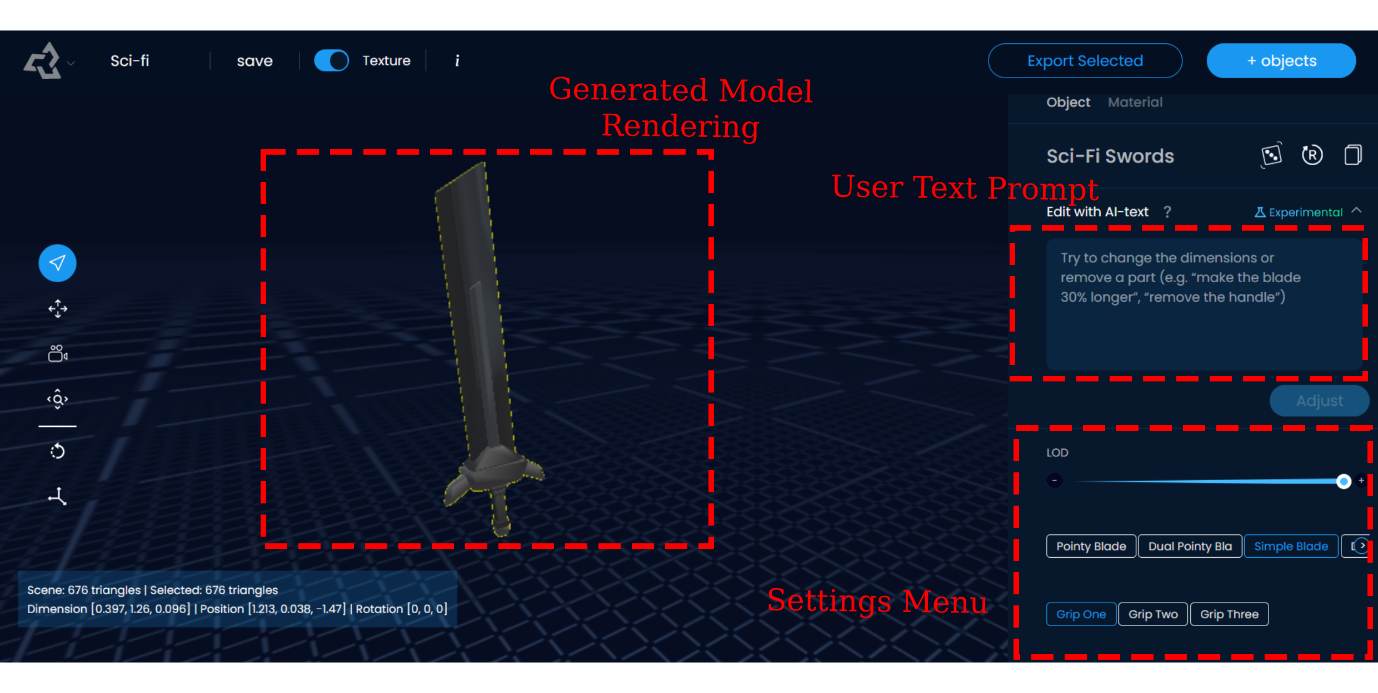
\includegraphics[width=6.25694in,height=2.87255in]{MyThesisImages/media/image75.png}
    \caption{SLOYD AI playground interface.}
\end{figure}

\textbf{Settings Menu approach}

Sloyd offers an interactive menu comprised of sliders, buttons and check-boxes. By changing any of those elements, users can create great variation by enabling/disabling certain features, setting different slider variables and choosing between available component variations of the object they are attempting to generate.\\

\textbf{{Text-Prompt approach}}

The user can provide a text-prompt describing the desired
characteristics of the object he is trying to generate, and the AI tool
will automatically change the sliders or enable/disable components.

It is important to mention that this method requires the user to study
the different components of the object he is trying to generate a
variation of and explain in detail the variable he wants to change.

After much experimentation with the text-prompt system it was concluded
that the best approach is to prompt Sloyd to generate the model without
mentioning any detail characteristics and after the model is generated
prompt in the "Edit with AI-text" menu option and prompt the AI to
change the components of the model or dimensions of them.

Generate a model Text-prompt examples:

\begin{itemize}
\item
  "Laser Blaster"
\item
  "Sword"
\item
  "Drone"
\end{itemize}

Edit a model Text-prompt examples:

\begin{itemize}
\item
  Sword -- "Dual Angled, blade 0.8 length, tapered grip, enable grip
  end detail, pyramid grip end detail."
\item
  Laser Blaser- "antennae barrel, round back, elaborate handle,
  enable barrel antenna, antenna 0.5 length."
\end{itemize}

\textbf{{Export Process}}

After generating the desired object, the user can export it for use
outside of the Sloyd environment.

All objects generated by Sloyd come pre-textured with simple materials
and a large assortment of different palettes of material presets is
available. Users can export the entire model including the mesh and
textures or can opt for the mesh only export option and texture the
model themselves in a different software of choice.

Export file format:

\begin{itemize}
\item
  .OBJ - combines all component meshes into one mesh and exports it
  without any material.
\item
  .GLB -- Exports the model as individual separate components including
  all the materials
\end{itemize}

It is recommended to export the model as GLB format and join the meshes
in a separate modeler software as well as perform changes in the
material slots or set appropriate mesh origin as needed.


\subsection{(Section 5.2.b) Textures -- Polycam and Real-ESRGAN}
\begin{enumerate}
\def\labelenumi{\arabic{enumi}.}
\item
  \textbf{{Texture Generation}}
\end{enumerate}

Polycam \cite{polycam} is a company that offers a variety of different tools for free
public use on their website. Their primary focus is Lidar photography
and photogrammetry, but they also offer a text-prompt based AI texture
generator that also includes image-to-image generation. 
\begin{figure}[H]
	\centering
    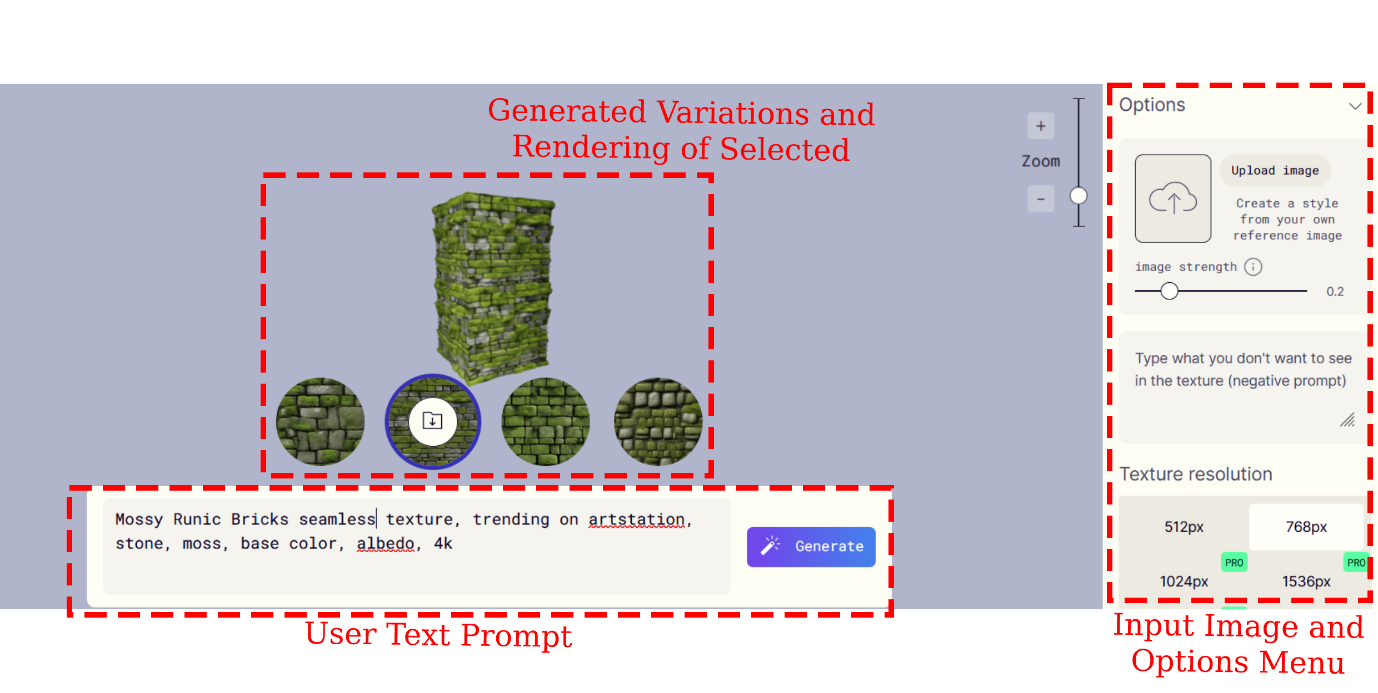
\includegraphics[width=6.25694in,height=2.77083in]{MyThesisImages/media/image76.png}
    \caption{Polycam Texture Generator interface. Prompt is used to
generate 4 different variations of the described texture.}
\end{figure}

The texture generation process is very simple. The user provides the AI
with a set of keywords that describe the desired texture, and the tool
generates four different variations based on them as well as showing a
rendered preview of the PBR material rendered on top of a cuboid.

Another way of generating a texture is by using an existing image as an
input sample for the AI to reference, fine-tuned with a variable that
controls how close to the reference image should the generated texture
be.

The AI texture generator is not only generating the color map, also
known as albedo, but also generates the Normal, Displacement and
Roughness maps.

This is an important distinction between image and texture generators,
as the albedo alone cannot create a good result on the PBR material
workflow. The results are flat and lack realism when rendered on top of
3D surfaces.

Another aspect of the polycam texture generator is that all textures generated from this 
tool are seamless and can be infinitely tiled on 3d
surfaces without a noticeable seam.\newline

Example of prompts and generated results:


\begin{table}[H]
    \centering  
    \begin{tabular}
    {|m{5.5em}||m{6.8em}||m{6.8em}||m{6.8em}|m{6.8em}|}
    \hline
Albedo &\raisebox{-0.5cm}{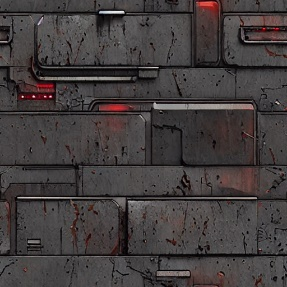
\includegraphics[width=3cm, height=3cm]{MyThesisImages/media/image77.jpeg}}&
\raisebox{-0.5cm}{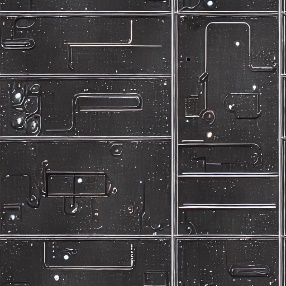
\includegraphics[width=3cm, height=3cm]{MyThesisImages/media/image78.jpeg}}&
\raisebox{-0.5cm}{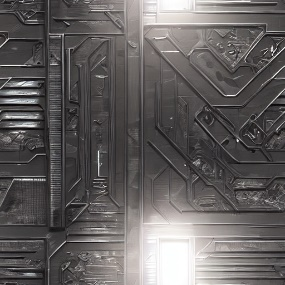
\includegraphics[width=3cm, height=3cm]{MyThesisImages/media/image79.jpeg}}&
\raisebox{-0.5cm}{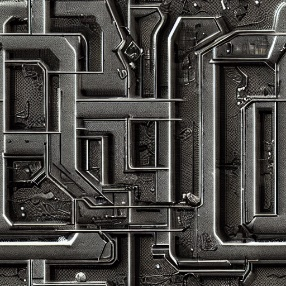
\includegraphics[width=3cm, height=3cm]{MyThesisImages/media/image80.jpeg}}\\
    \hline
Normals &\raisebox{-0.5cm}{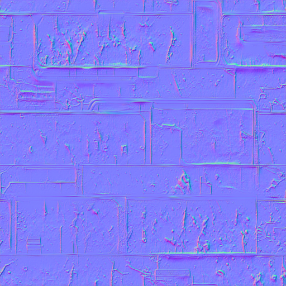
\includegraphics[width=3cm, height=3cm]{MyThesisImages/media/image81.png}}&
\raisebox{-0.5cm}{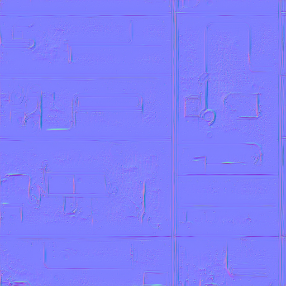
\includegraphics[width=3cm, height=3cm]{MyThesisImages/media/image82.png}}&
\raisebox{-0.5cm}{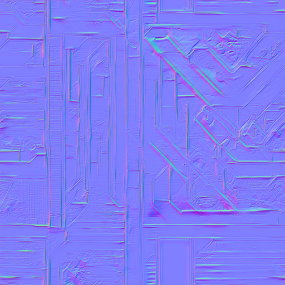
\includegraphics[width=3cm, height=3cm]{MyThesisImages/media/image83.png}}&
\raisebox{-0.5cm}{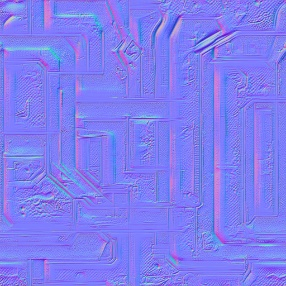
\includegraphics[width=3cm, height=3cm]{MyThesisImages/media/image84.jpeg}}\\
 \hline
Roughness &\raisebox{-0.5cm}{
\includegraphics[width=3cm, height=3cm]{MyThesisImages/media/image85.jpeg}}&
\raisebox{-0.5cm}{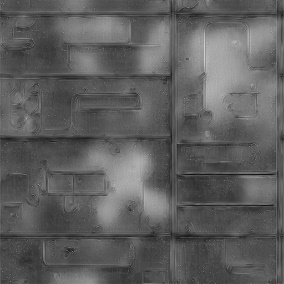
\includegraphics[width=3cm, height=3cm]{MyThesisImages/media/image86.jpeg}}&
\raisebox{-0.5cm}{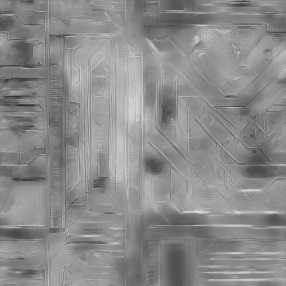
\includegraphics[width=3cm, height=3cm]{MyThesisImages/media/image87.jpeg}}&
\raisebox{-0.5cm}{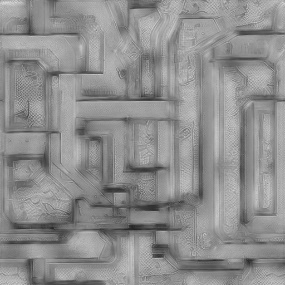
\includegraphics[width=3cm, height=3cm]{MyThesisImages/media/image88.jpeg}}\\
 \hline
Displacement &\raisebox{-0.5cm}{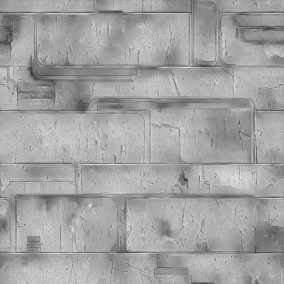
\includegraphics[width=3cm, height=3cm]{MyThesisImages/media/image89.jpeg}}&
\raisebox{-0.5cm}{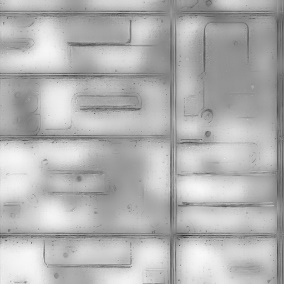
\includegraphics[width=3cm, height=3cm]{MyThesisImages/media/image90.jpeg}}&
\raisebox{-0.5cm}{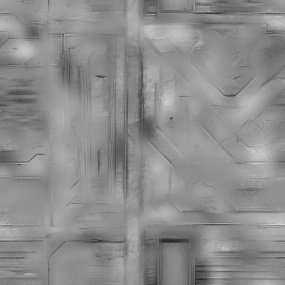
\includegraphics[width=3cm, height=3cm]{MyThesisImages/media/image91.jpeg}}&
\raisebox{-0.5cm}{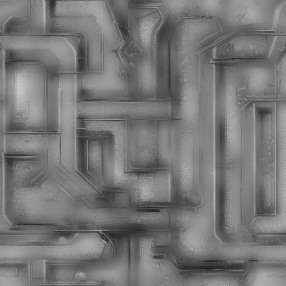
\includegraphics[width=3cm, height=3cm]{MyThesisImages/media/image92.jpeg}}\\
\hline
    \end{tabular}
    \caption{ Prompt: "Cyberpunk, metal, wall panel, sci fi, technology"}
\end{table} 


\begin{longtable}[H]
    {|m{5.5em}||m{6.7em}||m{6.7em}||m{6.7em}|m{6.7em}|}
    \hline
Albedo &\raisebox{-0.5cm}{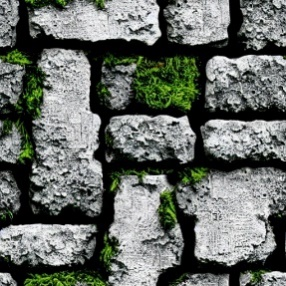
\includegraphics[width=3cm, height=3cm]{MyThesisImages/media/image93.jpeg}}&
\raisebox{-0.5cm}{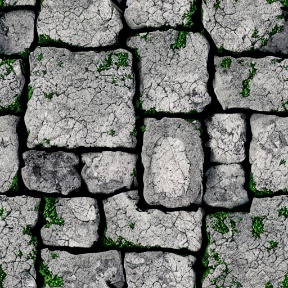
\includegraphics[width=3cm, height=3cm]{MyThesisImages/media/image94.jpeg}}&
\raisebox{-0.5cm}{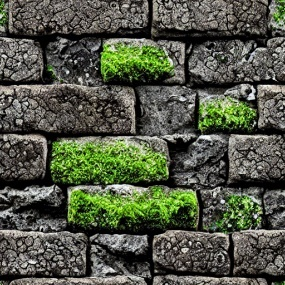
\includegraphics[width=3cm, height=3cm]{MyThesisImages/media/image95.jpeg}}&
\raisebox{-0.5cm}{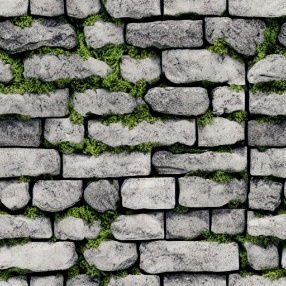
\includegraphics[width=3cm, height=3cm]{MyThesisImages/media/image96.jpeg}}\\
    \hline
Normals &\raisebox{-0.5cm}{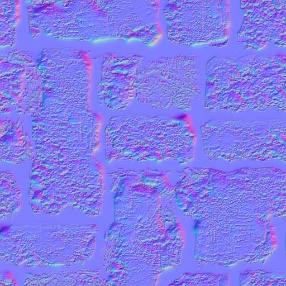
\includegraphics[width=3cm, height=3cm]{MyThesisImages/media/image97.jpeg}}&
\raisebox{-0.5cm}{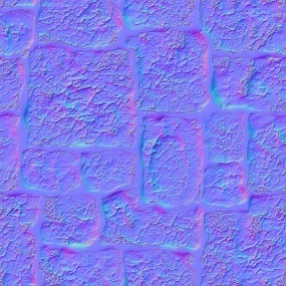
\includegraphics[width=3cm, height=3cm]{MyThesisImages/media/image98.jpeg}}&
\raisebox{-0.5cm}{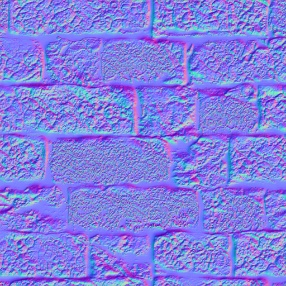
\includegraphics[width=3cm, height=3cm]{MyThesisImages/media/image99.jpeg}}&
\raisebox{-0.5cm}{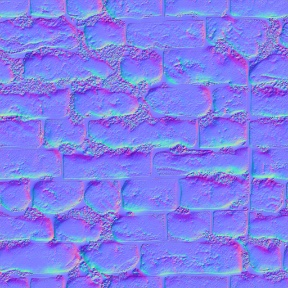
\includegraphics[width=3cm, height=3cm]{MyThesisImages/media/image100.jpeg}}\\
 \hline
Roughness &\raisebox{-0.5cm}{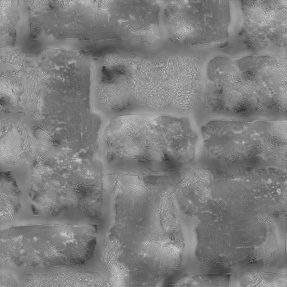
\includegraphics[width=3cm, height=3cm]{MyThesisImages/media/image101.jpeg}}&
\raisebox{-0.5cm}{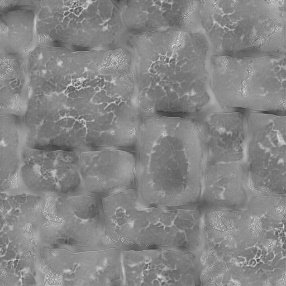
\includegraphics[width=3cm, height=3cm]{MyThesisImages/media/image102.jpeg}}&
\raisebox{-0.5cm}{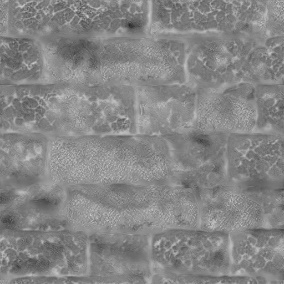
\includegraphics[width=3cm, height=3cm]{MyThesisImages/media/image103.jpeg}}&
\raisebox{-0.5cm}{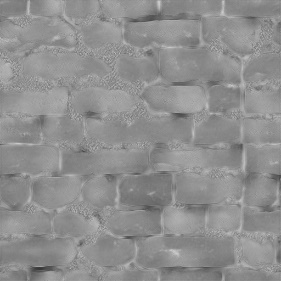
\includegraphics[width=3cm, height=3cm]{MyThesisImages/media/image104.jpeg}}\\
 \hline
Displacement &\raisebox{-0.5cm}{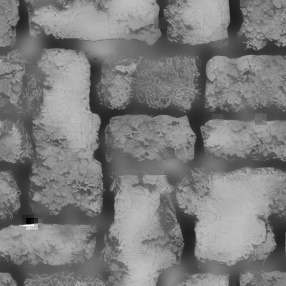
\includegraphics[width=3cm, height=3cm]{MyThesisImages/media/image105.jpeg}}&
\raisebox{-0.5cm}{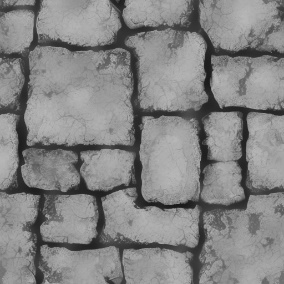
\includegraphics[width=3cm, height=3cm]{MyThesisImages/media/image106.jpeg}}&
\raisebox{-0.5cm}{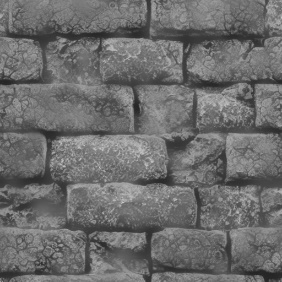
\includegraphics[width=3cm, height=3cm]{MyThesisImages/media/image107.jpeg}}&
\raisebox{-0.5cm}{
\includegraphics[width=3cm, height=3cm]{MyThesisImages/media/image108.jpeg}}\\
\hline
    \caption{ Prompt: "Mossy Runic Bricks, stone, moss"}
\end{longtable} 

\begin{enumerate}
\def\labelenumi{\arabic{enumi}.}
\setcounter{enumi}{1}
\item
  \textbf{{Texture Upscaling}}
\end{enumerate}

After generating the desired textures and corresponding maps, we could
immediately import them inside the game engine of choice and use them to
render the PBR material. The problem is that the Polycam AI texture
generator creates and exports images in 512x512 resolution (on the free
version) which for modern game development is considered to be a very
low resolution.

In order to solve this problem, we need to utilize a super resolution
technique on your generated textures. An online implementation of the
ESR-GAN \cite{wang_2019_esrgan} that was discussed in the second chapter of the thesis
will be used to make the individual texture images in higher resolution
before importing them into the game engine. The Real-ESRGAN AI tool
\cite{realesrgan} offers the option to upscale 2x, 4x and 8x super resolution,
so in this case we can go from 512x512 to 1024x124 to 2048x2048 or
4096x4096 resolution.
\begin{figure}[H]
	\centering
    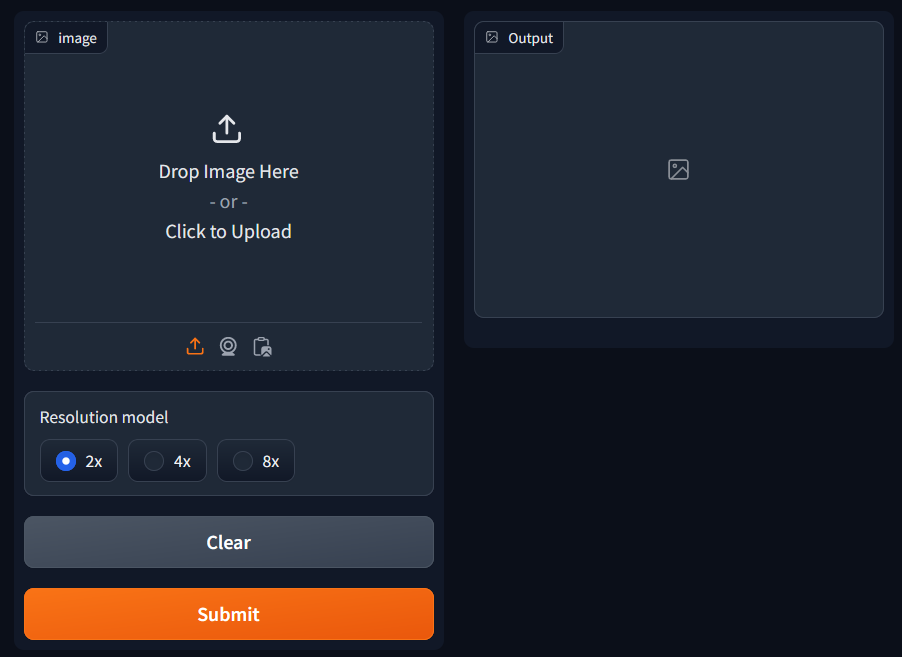
\includegraphics[width=3.53788in,height=2.57518in]{MyThesisImages/media/image109.png}
    \caption{Real-ESRGAN playground interface. Source:\cite{realesrgan}}
\end{figure}

For the purpose of developing a game inside unreal engine only the
albedo, normal and roughness maps will be upscaled to 2048x2048 and
utilized in the PBR workflow.


\begin{longtable}[H]
    {|m{14.3em}||m{14.3em}|}
    \hline
\raisebox{-0.5cm}{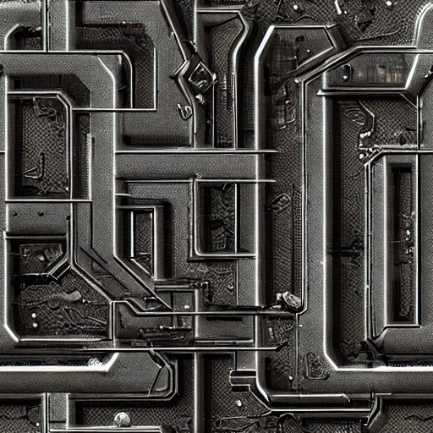
\includegraphics[width=6cm, height=6cm]{MyThesisImages/media/image110.jpeg}}&
\raisebox{-0.5cm}{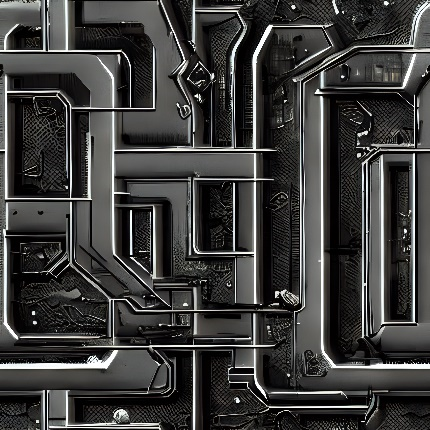
\includegraphics[width=6cm, height=6cm]{MyThesisImages/media/image111.jpeg}}\\
    \hline
\raisebox{-0.5cm}{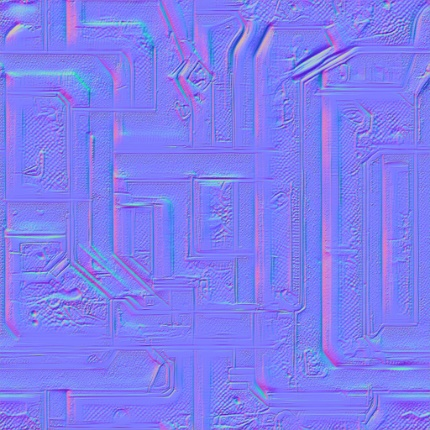
\includegraphics[width=6cm, height=6cm]{MyThesisImages/media/image112.jpeg}}&
\raisebox{-0.5cm}{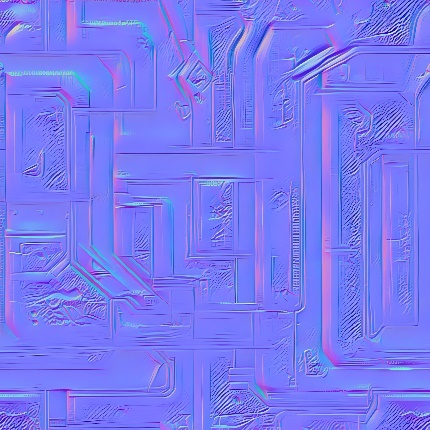
\includegraphics[width=6cm, height=6cm]{MyThesisImages/media/image113.jpeg}}\\
 \hline
\raisebox{-0.5cm}{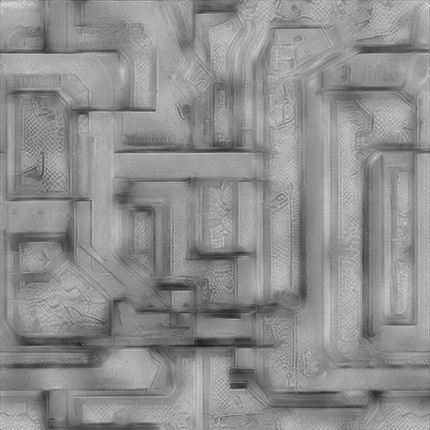
\includegraphics[width=6cm, height=6cm]{MyThesisImages/media/image114.jpeg}}&
\raisebox{-0.5cm}{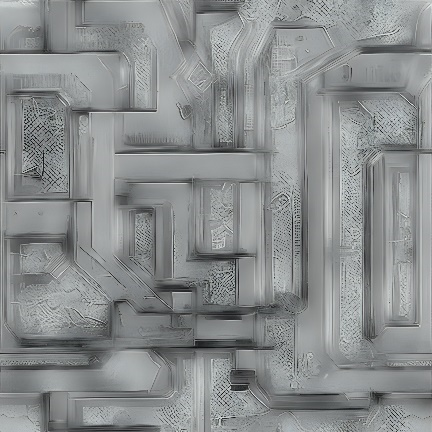
\includegraphics[width=6cm, height=6cm]{MyThesisImages/media/image115.jpeg}} \\
\hline
    \caption{ Left the generated 512x512 textures. Right their upscaled
versions of Real-ESRGAN
}
\end{longtable} 
The quality of the upscaled textures is outstanding, with no observable
artifacts from the Real-ESRGAN method. It produces a crisper image while
are the same time removes artifacts produced by the texture generation
model.

With careful examination, it can be seen that some details have been
lost in the normal map upscaled texture, most likely because the model
was not trained specifically with texture generation and the original
image is of low resolution. Nevertheless, the model performs better than
expected in texture upscaling compared to other methods tested (e.g.
Pixelcut Upscaler AI\cite{pixelcut}) which left many artifacts in the final image.

\begin{figure}[H]
	\centering
    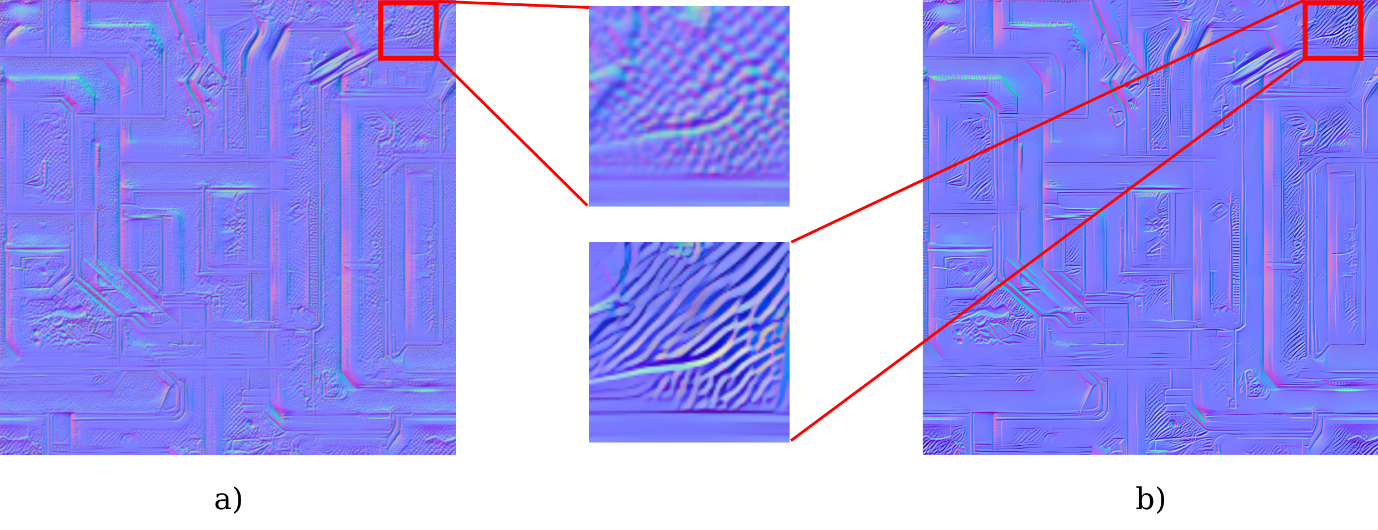
\includegraphics[width=5.25833in,height=2in]{MyThesisImages/media/image116.png}
    \caption{ a) Original generated texture b) Real-ESRGAN upscaled version.}
\end{figure}

\subsection{(Section 5.2.c) Audio -- SOUNDRAW, Stable Audio and EvokeMusic}

Audio can be separated in two categories:
\begin{itemize}
\item 
  \textbf{Music}
\item
  \textbf{Sound Effects}
\end{itemize}


\paragraph{Music - SOUNDRAW\newline \newline }

For generating music, the SOUNDRAW AI\cite{soundraw} will be used as it
offers a better environment for real time editing of the generated music
than other similar music generating AI tools.

In order to generate music, the SOUNDRAW AI has a tag-based approach.
The user must select one or more tags that describe the characteristics
of the music track he wants, and the AI generates a list of song tracks
obeying the selected tags.

\begin{figure}[H]
	\centering
    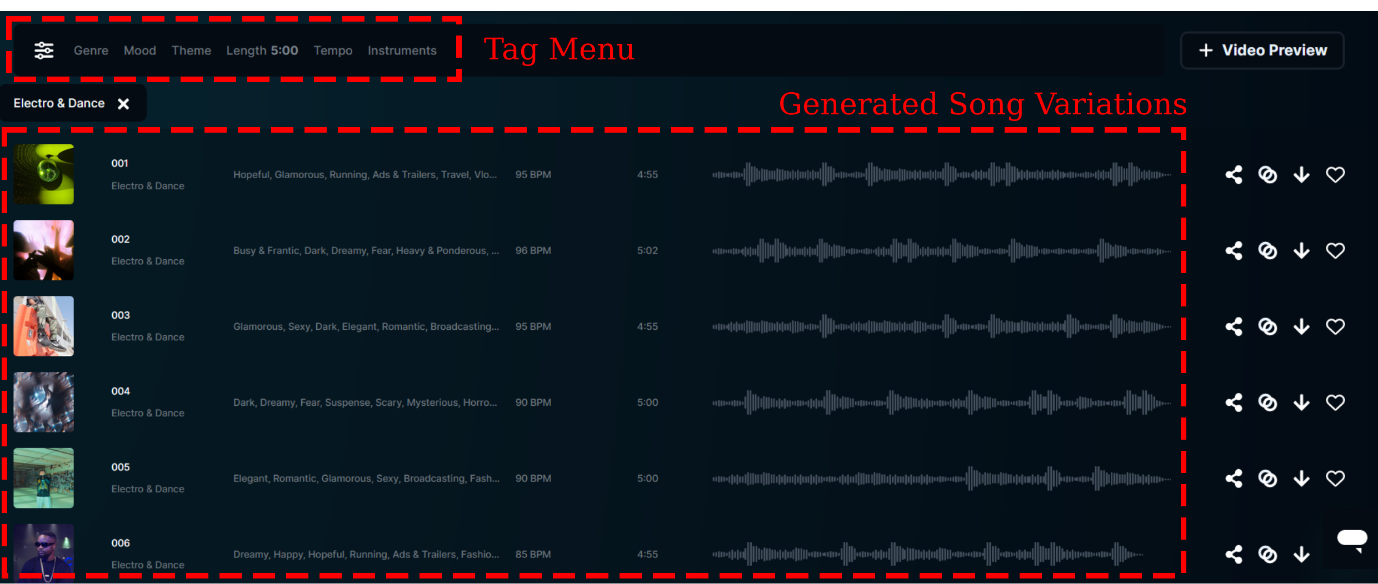
\includegraphics[width=6.25833in,height=2.64167in]{MyThesisImages/media/image117.png}
    \caption{ Soundraw Interface.}
\end{figure}

\textbf{Tag Categories}


\begin{enumerate}
\def\labelenumi{\arabic{enumi}.}
\item
  Genre 
  \begin{quote}
      Hip-Hop, Drill, Trap, R\&B, Jersey Club, Latin, Acoustic, Rock, Ambient, Beats, Drum n Bass, Electro \& Dance, Funk, House, Techno \& Trance, Tokyo night pop, Pop, Lofi Hip Hop, World, Electronica, Orchestra, Tropical House, Afrobeats, Phonk, Christmas
  \end{quote}
\item 
    Mood 
    \begin{quote}
        Epic, Happy, Hopeful, Laid Back, Angry, Sentimental, Busy \& Frantic, Romantic, Funny \& Weird, Dark, Glamorous, Mysterious, Elegant, Dreamy Euphoric, Fear, Heavy \& Ponderous, Peaceful, Restless, Running, Sad, Scary, Smooth, Suspense 
    \end{quote}
\item
  Theme 
  \begin{quote}
      Corporate, Photography, Motivational\& Inspiring, Cinematic, Comedy, Cooking, Fashion\& Beauty, Nature, Sports \& Action, Technology, Tutorials, Travel, Workout \& Wellness, Gaming, Wedding \& Romance, Horror \& Thriller, Ads \& Trailers, Broadcasting, Holiday Season, Drama, Documentary, Vlogs
  \end{quote}
\item
  Length 
  \begin{quote}
      10sec, 15sec, 1min, 1:30min,2min,3min,4min,5min
  \end{quote}
\item
  Tempo 
  \begin{quote}
      Slow, Normal, Fast
  \end{quote}
\item Instruments 
    \begin{quote}
        Piano, Keyboard, Synth, Acoustic Guitar, Electric Guitar, Bell, Maller, Ethnic, Strings, Voice, Brass, Woodwind 
        \end{quote}
\end{enumerate}

By choosing one or more tags from the Genre, Mood, and Theme categories
the user can make more specific generations.

The Length tag sets the approximate length of time the tracks will have.

The Tempo tag specifies to the AI the approximate maximum Beats per
Minute or BPM the generated music should have.

The Instruments tag, enables or disables instruments included in the
generated music. The AI will automatically choose all available
instruments depending on the other tags chosen previously but the user
can keep only those he wants.

After choosing a tag from a category, some tags from the other
categories may be be excluded automatically and the user will have to
choose from the other available choices. Making combinations of tags
that relate closer to one another will produce more desirable results.\\

\textbf{Example of Tag list}

\begin{itemize}
\item
  Genre - Electro \& Dance
\item
  Mood - Dark, Gaming
\item
  Length - 5mins
\item
  Tempo - slow/normal/fast tempo
\item
  Instruments - piano, keyboard, synth, electric guitar, strings, voice,
  brass
\end{itemize}

After generating the music and finding a desirable track, the user has
the option to generate similar music based on the track selected.\\

\textbf{Track Editing}

After generating and selecting the desired track, Soundraw offers the
ability to edit it. The generated track is sliced in equal time
intervals and the user can change the characteristics of each segment in
the edit menu.

Moreover, the user has access to each segment's component level editing
such us Melody, Backing, Bass, Drums, Fills and can edit them
individually.

The available options are:

\begin{itemize}
\item
  duplicate segment.
\item
  delete segment.
\item
  change component energy level.
\item
  Increase/Decrease track length
\item
  3 choices to change BPM.
\item
  3 choices to change instrument for each component.
\item
  3 choices to change Key.
\item
  Component Volume control.
\end{itemize}

\begin{figure}[H]
	\centering
    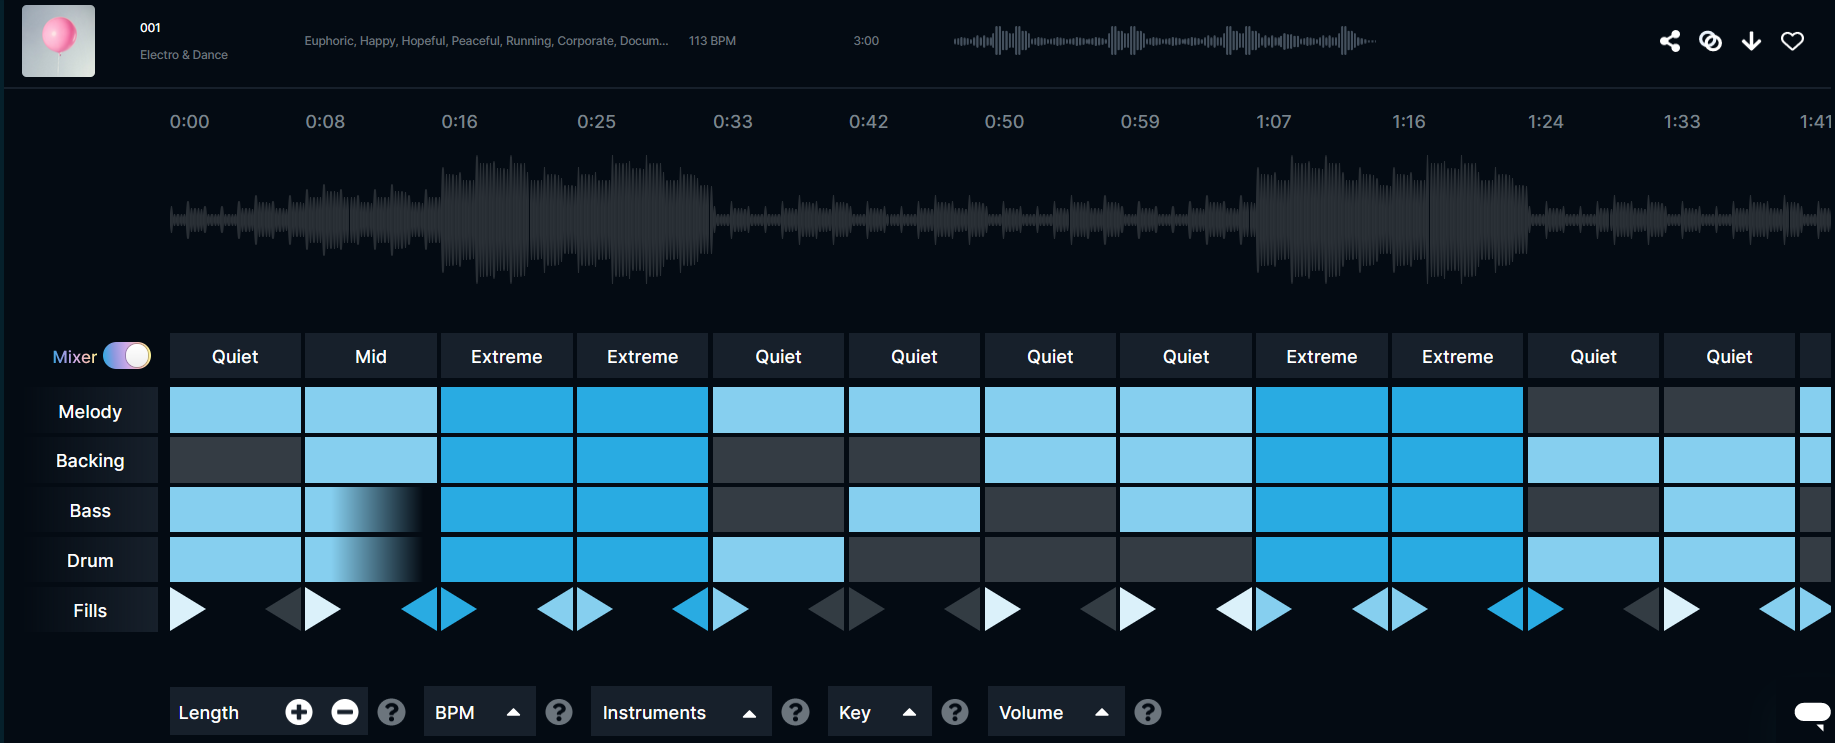
\includegraphics[width=6.25833in,height=2.53333in]{MyThesisImages/media/image118.png}
    \caption{ Soundraw Track Editing Interface.}
\end{figure}

After editing the track and reaching the desired result the song can be
downloaded and used royalty free in any project. Soundraw offers a
variety of export file formats like MIDI, MP3, WAV etc. The recommended
type is WAV as it's the standard lossless, uncompressed format supported
by almost every software.


\paragraph{Sound Effects -- STABLE AUDIO and EVOKE MUSIC}

\begin{enumerate}
\def\labelenumi{\arabic{enumi}.}
\item
  \textbf{Stable Audio}
\end{enumerate}

\begin{quote}
Stable Audio which was discussed in technical detail in the literature
review part of the thesis, is an audio generating AI, capable of
creating music as well as sound effects in high quality, by using a
text-based prompt system as well as audio-to-audio generation.
\cite{evans_2024_fast, stable_audio}

It supports variable length stereo audio generation with maximum of 90
seconds with the AudioSparx 1.0 dataset and 180 seconds with the new
AudioSparx 2.0.

The audio-to-audio feature supports maximum of 3 minutes input audio.

\begin{figure}[H]
	\centering
    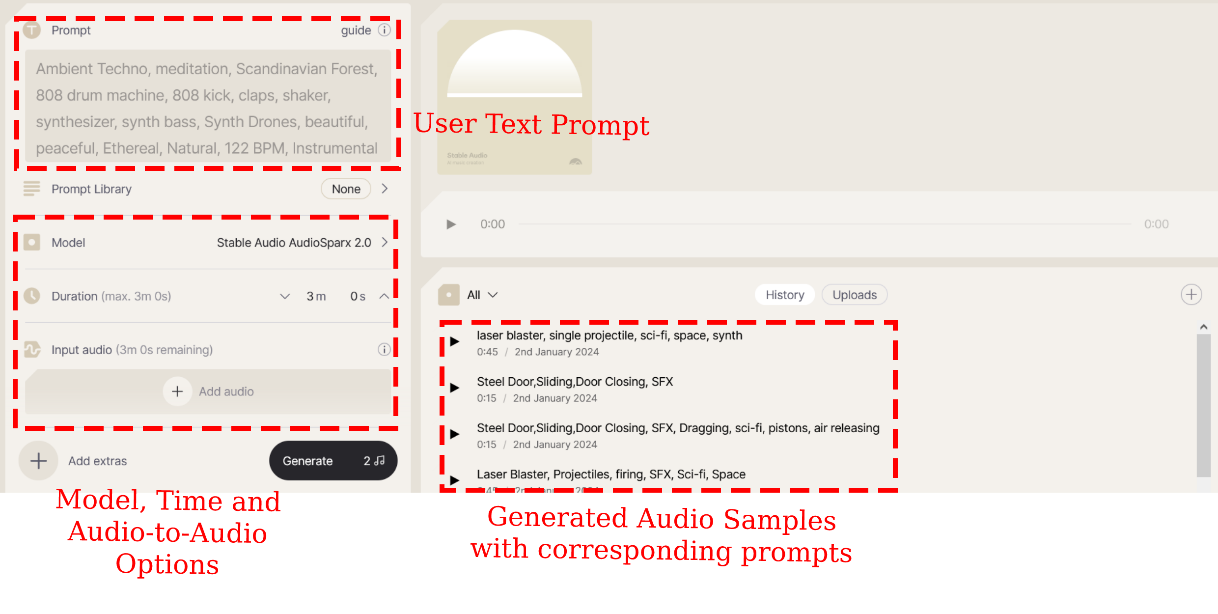
\includegraphics[width=5.51962in,height=2.63889in]{MyThesisImages/media/image119.png}
    \caption{Stable Audio Interface.}
\end{figure} 
\end{quote}


\textbf{Text-prompt construction}

The more detailed the text prompt is the more specific the generated
track will be, a good prompt must include descriptive words and phrases
in order to guide the AI properly.

A combination of musical and emotional terms, setting, instruments and
tempo will produce a very specific generation.

Prompt example:


\begin{itemize}
\item
  \emph{"Dark, Sci-fi, Gaming, Atmospheric, Electronic music, Beats,
  Synth, Electric guitar, Bass, Drums, Action, Suspense"}
\item
  \emph{"Laser Blaster, Single Projectile, SFX, Sci-fi, Space, synth"}
\item
  \emph{"Steel Door Sliding, Dragging, Door Closing, Sci-fi, SFX"}
\end{itemize}

Before generating you can choose the duration of the track in seconds,
minding of course the limits of the subscription package.

After generating the and selecting the desired track, it can be exported
in MP3 or WAV formats.

As mentioned before, the free subscription package doesn't allow
commercial use of the content generated, only the professional and
enterprise packages allow for commercial use of the generated
soundtracks.

\begin{enumerate}
\def\labelenumi{\arabic{enumi}.}
\setcounter{enumi}{1}
\item
  \textbf{Evoke Music}
\end{enumerate}

A different approach is to utilize Evoke Music\cite{Evoke}, an online
library comprised by collection of over 60.000 different royalty songs
and sound effects created and composed by the company's proprietary
Artificial Intelligence songwriting model named Amadeus Code.

The user has access to the AI generated content and is able to browse
the website or search manually using key words that describe the song or
sound effect he wants. Those key words can be genre, mood or instruments
included in the song and as for the sound effects they can be setting,
item or action.\\

\textbf{Examples of search prompts:}

\begin{itemize}
\item
  "Door, Sliding, wooden"
\item
  "Electric, Buzzer"
\item
  "Laser, gun, space, sci-fi
\item
  "Rock, Electric Guitar, Epic"
\item
  "Orchestral, heroic, strings"
\item
  "Electronic, beats, space, sci-fi"
\end{itemize}

The first tree examples are focused on SFX-sound effects and the latter
three on music, but every one of those will try to find results in both
categories.

A unique characteristic of Evoke Music is that every song generates is
comprised by smaller segments called loops and the user is able to
download not only entire songs but individual loops that he desires as
well.

Amadeus Code AI is powered by the Music Trinity Generative Algorithm or
MusicTGA. It is an artificial intelligence generative algorithm capable
of generating "rhythm, melody, and harmony based on "Licks," which
are minimal viable sound phrases". The data set used to generate music
and SFX is comprised of "9 million licks, of which 99.5\% are generated
by MusicTGA itself " \cite{Amadeus} and the rest 0.5\% are licks are
human-created by the company's employees.

\subsection{(Section 5.2.d) AI assistant - ChatGPT }

In order to have an AI personal assistant inside a videogame's
environment, we need to leverage the power of large language models and
more specifically OpenAI's ChatGPT. \cite{openai_chatgpt}

Communication with ChatGPT from inside the Unreal Engine, by using a
community Plugin created by Kellan Mythen, that allows to call the
OpenAI API. \cite{mythen_2023_openai}\\

\textbf{{ChatGPT Unreal Engine Integration Process}}

Step 1: Acquire a key for the OpenAI API.

Step 2: Download and Install the plugin inside the Unreal Engine
project.

Step 3: Access the library of functions created by the plugin.

Step 4: Implement the API call and response handling procedures as
desired.\\

The API requires an input string to prompt ChatGPT and responds back
with a string. How the game developers decide to handle the input and
the output is entirely dependent on them. Designing proper User
Interfaces for the user to provide input and then handle how the output
response is presented back, is very important for the game's immersion.


\subsection{(Section 5.2.d) Concept Art -- Stable Diffusion/Easy Diffusion }

While Stable Diffusion implementations are widely available on the
internet, running such a model locally requires high computational
capabilities on the users end, which can be problematic for indie
developers who have tight budgets and cannot afford the best hardware or
to rent cloud based virtual machines.

Gigantic Work \cite{easy_diff} has created a free online implementation of the
very popular Stable Diffusion model called Easy Diffusion. More
specifically they offer three different variations being:

\begin{itemize}
\item
  SD XL 1.0 Base
\item
  SD XL 1.0 Refiner
\item
  SD 1.5 Pruned EMA
\end{itemize}

Developers can leverage the capabilities of those models without the
need of running them natively, to create concept art for their games,
for the purpose of visualizing their ideas and experiment with different
ones, before spending resources and more importantly time to create them
by hand.

With Easy Diffusion its possible to generate images using text prompts
or image2image generation and the environment provided by Gigantic Works
allows access to all the needed variables for model parameterization
inside an intuitive layout for easy use even for someone totally
inexperienced.

\begin{figure}[H]
	\centering
    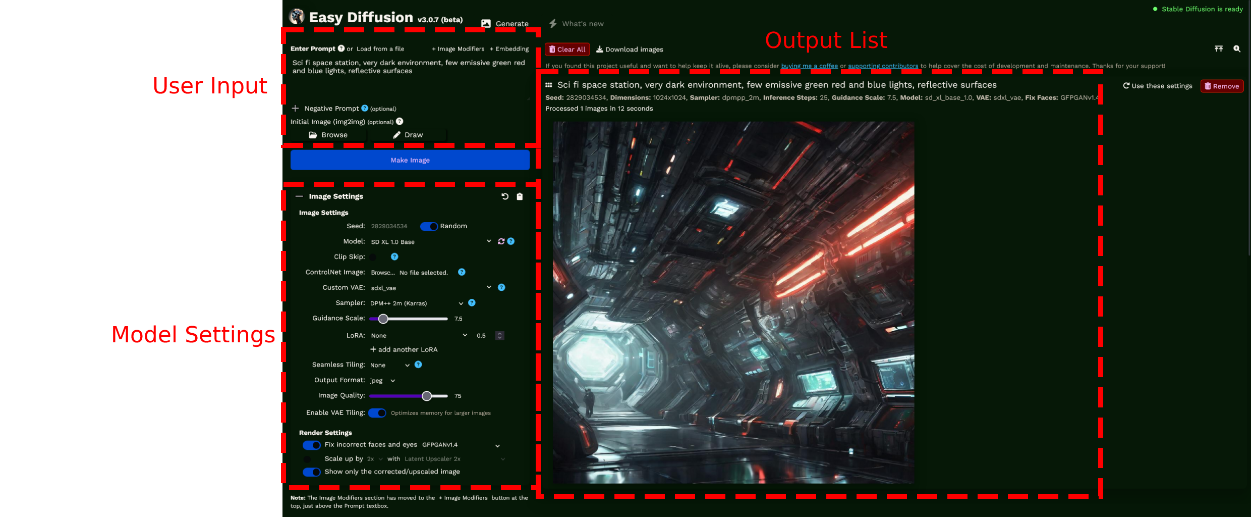
\includegraphics[width=5.67424in,height=2.34249in]{MyThesisImages/media/image120.png}
    \caption{Easy Diffusion Interface.}\label{fig:easydiff}
\end{figure} 

The interface provided by Easy Diffusion includes 3 main fields as shown
in figure \ref{fig:easydiff}.

\begin{itemize}
\item
  \textbf{User Input} Includes text prompt field, image input, user
  sketch input and image modifiers.
\item
  \textbf{Model Settings} Include all the necessary settings for
  controlling the model used for generation.
\item
  \textbf{Output List} Includes a history of all the previous prompts,
  as well as the corresponding settings and generated images for the
  current session.
\end{itemize}

Example prompts and generated images that was used as concept art for a
sci-fi space station environment:

\begin{figure}[H]
	\centering
    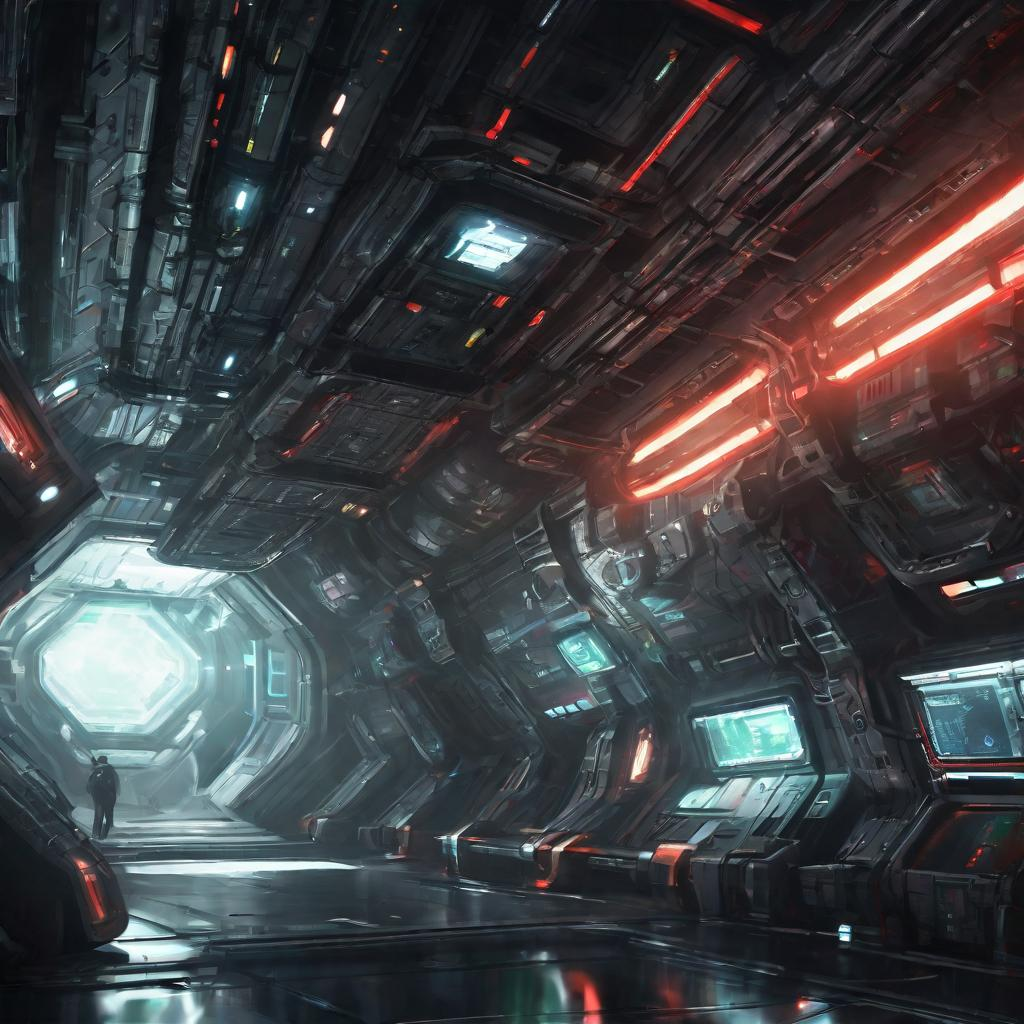
\includegraphics[width=3.20455in,height=3.20455in]{MyThesisImages/media/image121.jpeg}
    \caption{Prompt: "Sci fi space station, very dark environment, few emissive green red and blue lights, reflective surfaces"}
\end{figure} 

\begin{figure}[H]
	\centering
    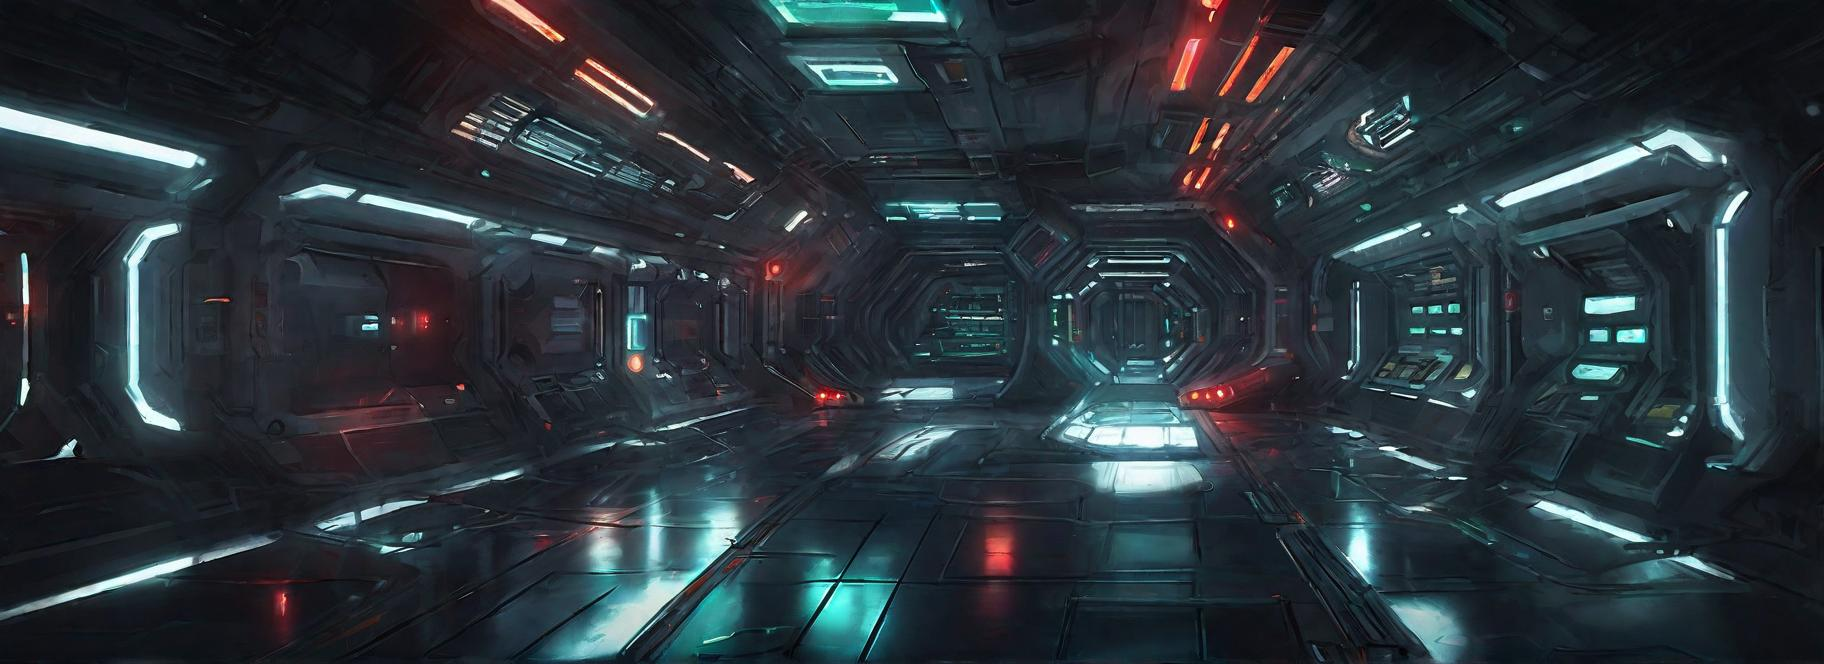
\includegraphics[width=6.25in,height=2.27292in]{MyThesisImages/media/image122.jpeg}
    \caption{Prompt: "Sci fi space station, very dark environment, few emissive green red and blue lights, reflective surfaces"}
\end{figure} 

\begin{figure}[H]
	\centering
    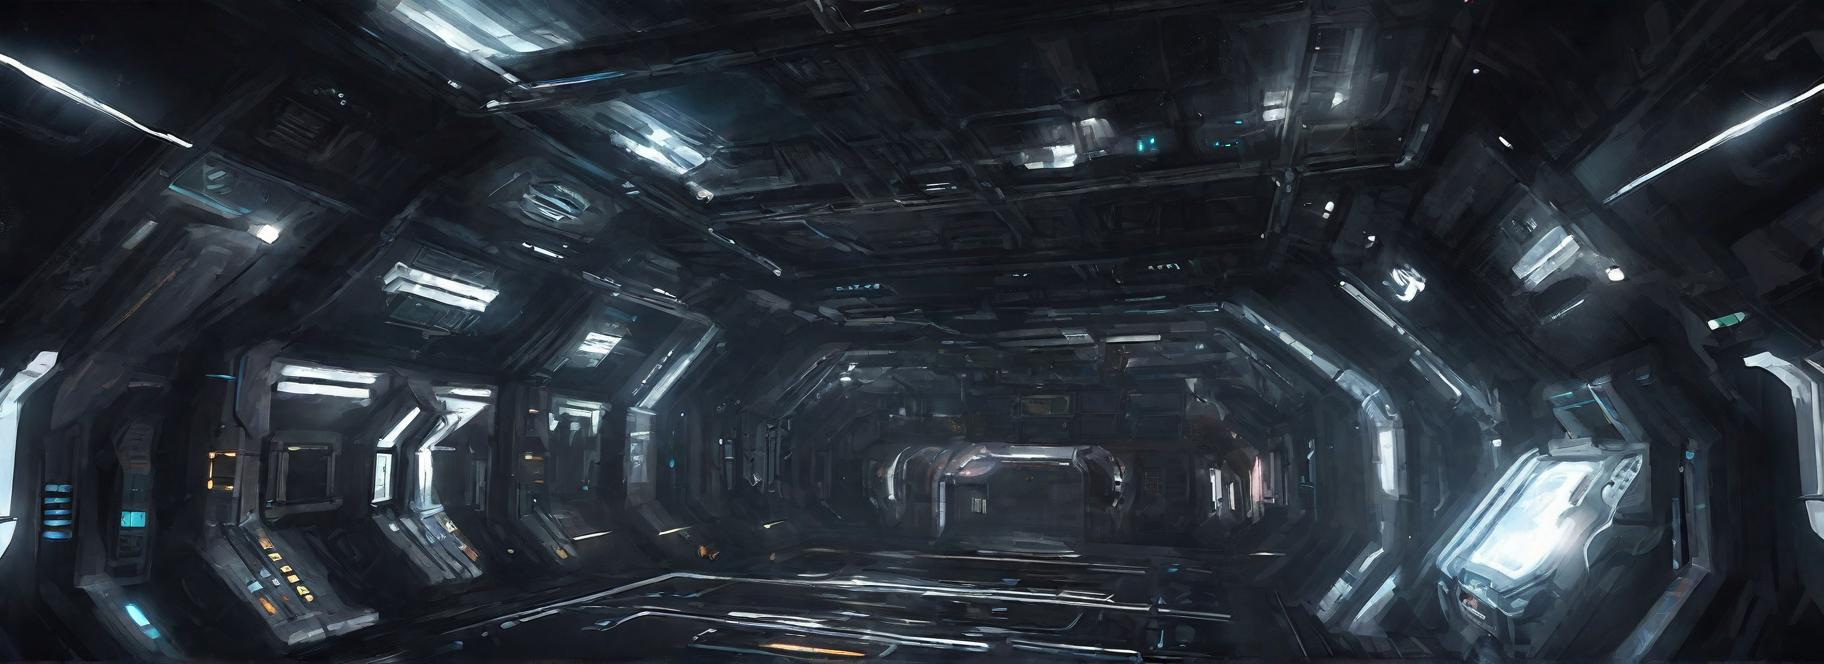
\includegraphics[width=6.25in,height=2.27292in]{MyThesisImages/media/image123.jpeg}
    \caption{Prompt: "Sci fi space station, dark environment, emissive lights"}
\end{figure} 


\section{(Sub-chapter 5.3) Chapter Conclusions }

In this chapter, an overview of the necessary software needed in video
game development was shown and available online AI tools that could
replace or speed-up considerably the developers' workflow were proposed
for use in game making.

Modern AI can offer a high degree of control in order to generate the
best result possible in correspondence with the developer vision of the
game.

With a focus on free or low-cost AI solutions developers can generate an
array of assets from objects to textures to audio for use, as prototypes
or as is, inside their video games.

It is a cutting-edge field of study that is constantly evolving with
each passing day. As people start using the different AI technologies,
scientists can collect even more data and slowly improve their models or
create better ones by analyzing and identifying weaknesses after large
scale public testing.

\begin{table}[H]
  \centering  
  \begin{tabular}
  {|m{4.1em}||m{2.5em}||m{5em}||m{5em}||m{5em}||m{5em}|}
  \hline
       Tool & Open\newline Source & Subscription\newline Based& Free\newline Generations	&Free\newline Generations\newline per month  & Commercial\newline Use\\
  \hline    
  \hline       					
Sloyd	&No	&Yes	&Yes	&3	&Yes	\\
\hline   
Soundraw	&No	&Yes	&Yes	&unlimited	&Yes\\
\hline   
Stable\newline Audio	&Yes	&Yes	&Yes	&10	&Yes\\
\hline   
Polycam	&No	&Yes	&Yes &unlimited	&Yes\\
\hline   
Real-\newline ESRGAN	&Yes	&No	&Yes	&unlimited	&Yes\\
\hline   
Easy\newline Diffusion	&Yes	&No	&Yes	&unlimited	&Yes\\

       \hline
  \end{tabular}
  \caption{The action space and low and high bounds
of each variable.}
\end{table} 

\pagebreak

\chapter{CHAPTER 6 Deep Reinforcement Learning inside Unreal Engine}

Gathering adequate amounts of data for training agents can be proven to be difficult depending on the task at hand. Discovering information
required to train agents in real world can be difficult and very
expensive or cost prohibitive in many cases, requiring specialized
equipment that has a chance to be damaged especially in the first stages of training while the agent learns the environment.

Modern video games can be a very detailed representation of the real
world inside a virtual space which enables easy access to every possible variable that might be needed. In this chapter the focus will be on a practical application of deep reinforcement learning (DRL) using a video game and leveraging the game-world as simulation environment for gathering input data to train an agent.

\section{(Sub-chapter 6.1) Agent Training inside Unreal Engine}

Unreal engine is one of the top free-access game engines, boasting many state-of-the-art features and a very active developer community, from big studios to indie teams and many individual developers.

Although it has some game AI features, state machines and a custom
implementation of behavior trees it does not include built-in deep
reinforcement learning capabilities. In order to train our agent, we
will use middleman approach. We extract the useful data from the game
world, encode and send them outside of the engine to be processed by a
deep reinforcement learning algorithm which will output a series of
actions for the agent to take, which will be send back to the engine.

\subsection{(Section 6.1.a) Introduction to the MIND MAKER plug-in}

Inspired by OpenAI Gym \cite{gym_openAI}, an API library enabling simulation and agent training inside python for general reinforcement learning
problems, Aaron Krumins created an engine plug-in for enabling
deployment of the same cutting-edge algorithms used in the OpenAI Gym
inside the engine environment called Mind Maker \cite{mindmaker}.

An important difference between the Mind Maker and OpenAI Gym is that
the latter is confined in training with old Atari Games, classic card
games and mostly 2D simulation environments, although there is an option of creating custom environments, it is limited to what pure coding can achieve. Mind maker on the other hand is focusing only on the connection between the unreal engine and the desired algorithm, therefor the possible virtual environments that can be created inside Unreal are endless. Making a transition from simple games and simulations to one of the most advanced and detailed world building platforms.

Mind Maker is based on a client-server approach thus it can used
natively in the same machine unreal is running on or it can be
configured to connect with a remote server, getting access to a
cloud-based system with more computational power when running larger
models.

Furthermore, Mind Maker can be used for Multi-Agent Reinforcement
Learning or MARL and work with multiple clients. It is as simple as
changing the port number, inside unreal, for each agent and the training can be done simultaneously and in parallel for up to 100 agents.

\subsection{(Section 6.1.b) Custom Environment for Agent Training }

For the purposes of training an agent inside the unreal engine a custom environment will be created from scratch using the generative AI tools discussed in the previous chapter.

List all AI generated assets used:

\begin{itemize}
\item
  3D models

  \begin{itemize}
  \item
    2 types of sci-fi Consoles
  \item
    Console screen(taken from the console model)
  \item
    Laser Gun
  \item
    Twin Barrel Gun
  \item
    2 types of Sci-fi crates
  \item
  \end{itemize}
\item
  Materials

  \begin{itemize}
  \item 2 Sci-fi Panels
  \item Sci-fi Panels with LED circuit board connections effect
  \item Console Screen with random texture and color based on mesh world location 
  \item Caustic texture effect
  \end{itemize}
\item
  Sounds

  \begin{itemize}
  \item
    10 background music tracks
  \item
    Hydraulic door opening
  \item
    Laser sound effect
  \item
    Shield whoosh
  \item
    Projectile explosion
  \item
    Shoot sound
  \item
    Multiple explosions
  \item
    Rolling sound
  \end{itemize}
\end{itemize}

\begin{figure}[H]
	\centering
    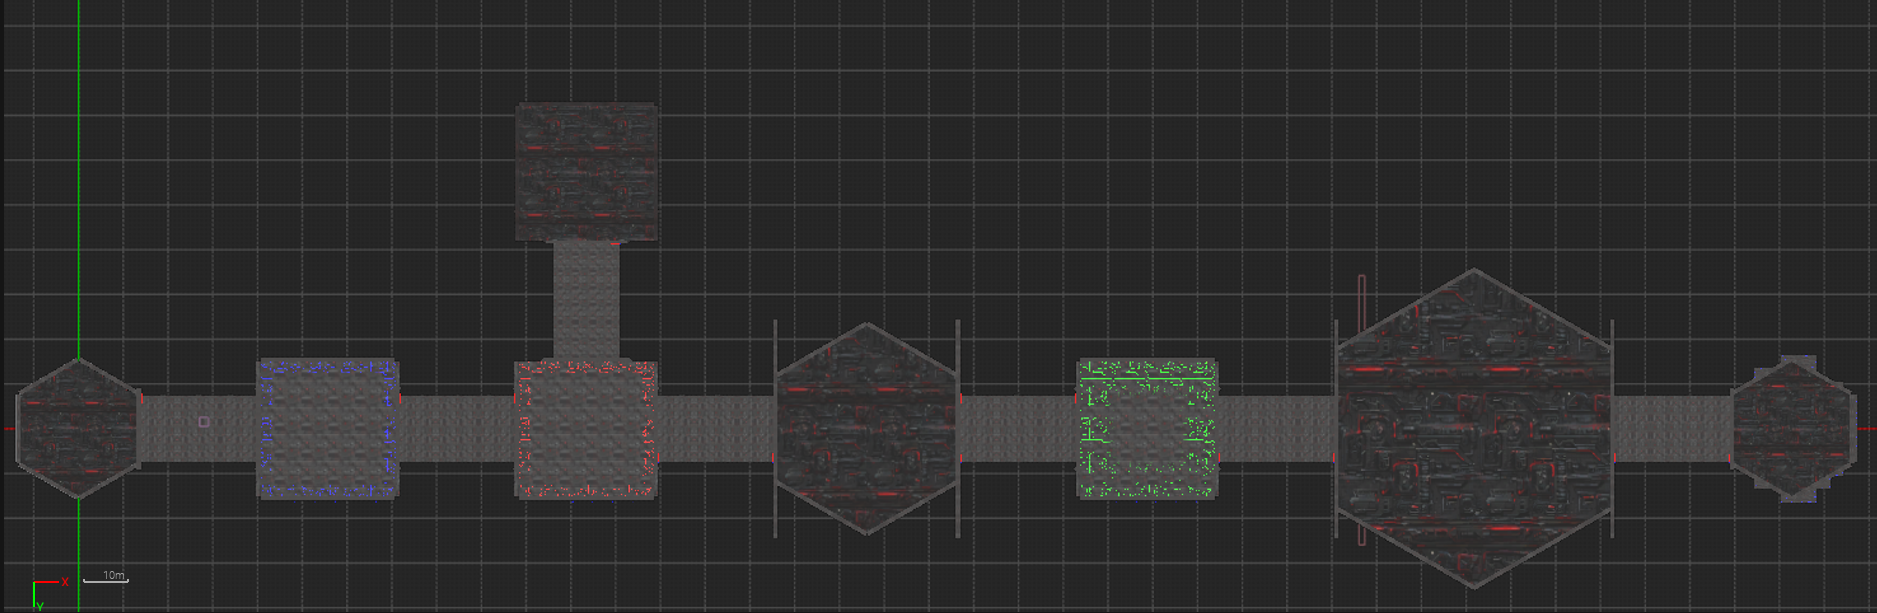
\includegraphics[width=6.25764in,height=2in]{MyThesisImages/media/agent training level.png}
    \caption{ Unlit top-view of the level to be used as a simulation environment.}
\end{figure} 

\begin{figure}[H]
	\centering
    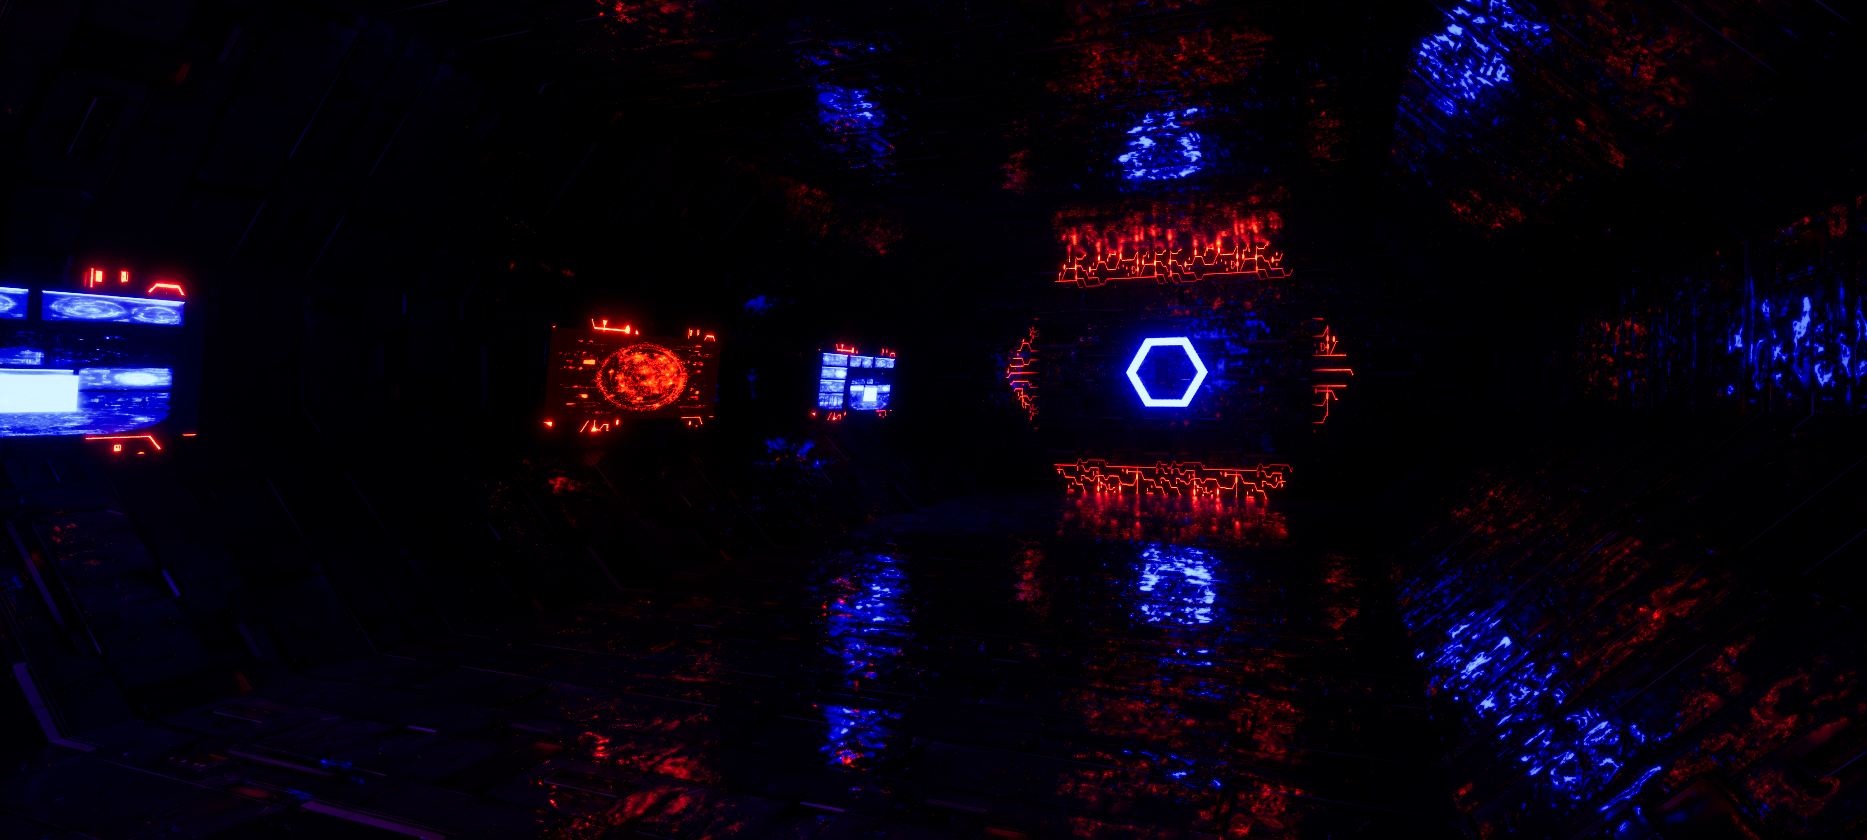
\includegraphics[width=6in,height=3in]{MyThesisImages/media/Agent Level 1.png}
    \caption{Screenshot 1 taken from the UE5 Simulation Environment.}
\end{figure} 

\begin{figure}[H]
	\centering
    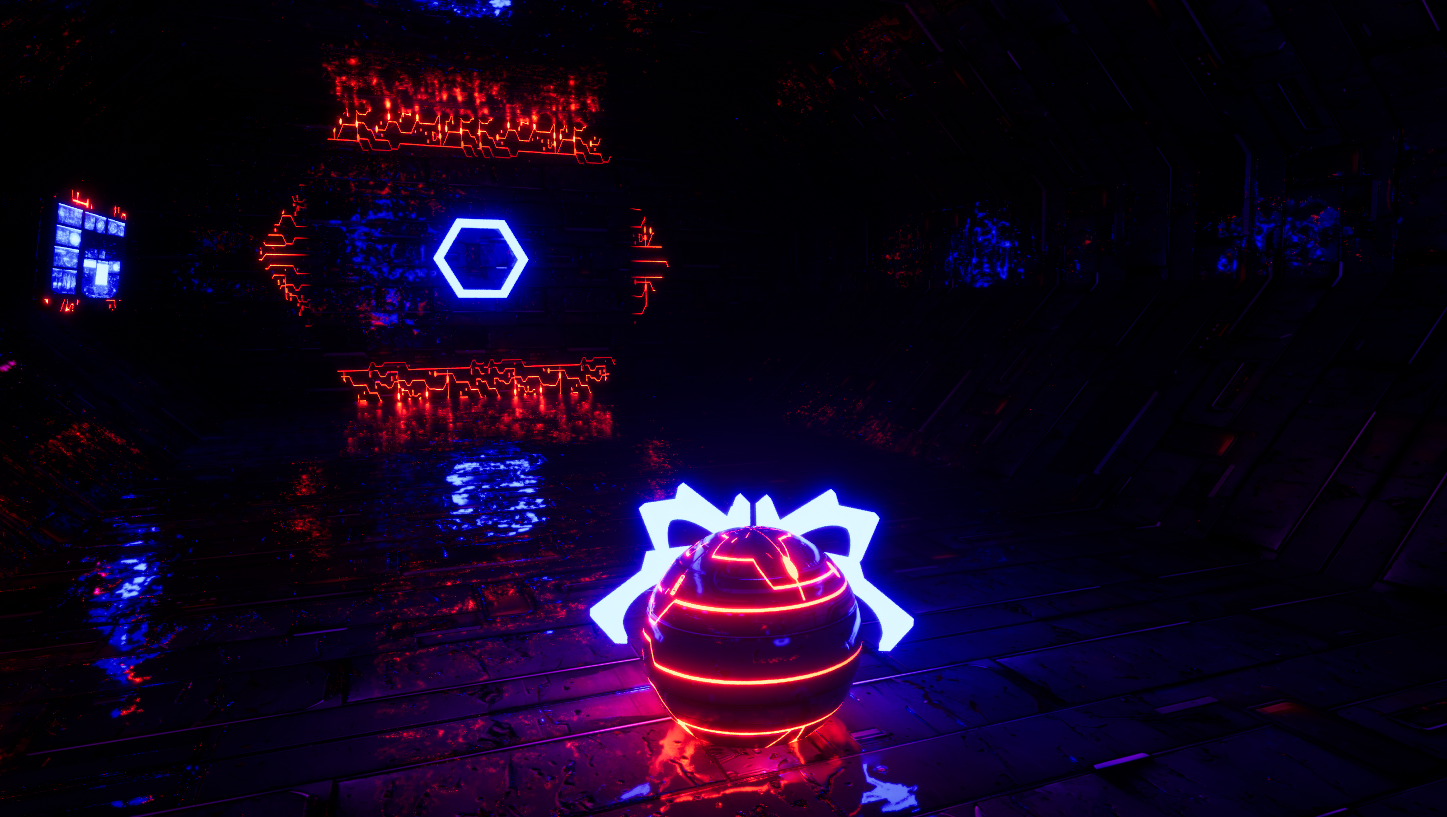
\includegraphics[width=5in,height=2.8in]{MyThesisImages/media/Agent Level 2.png}
    \caption{ Screenshot 2 taken from the UE5 Simulation Environment.}
\end{figure} 
\begin{figure}[H]
	\centering
    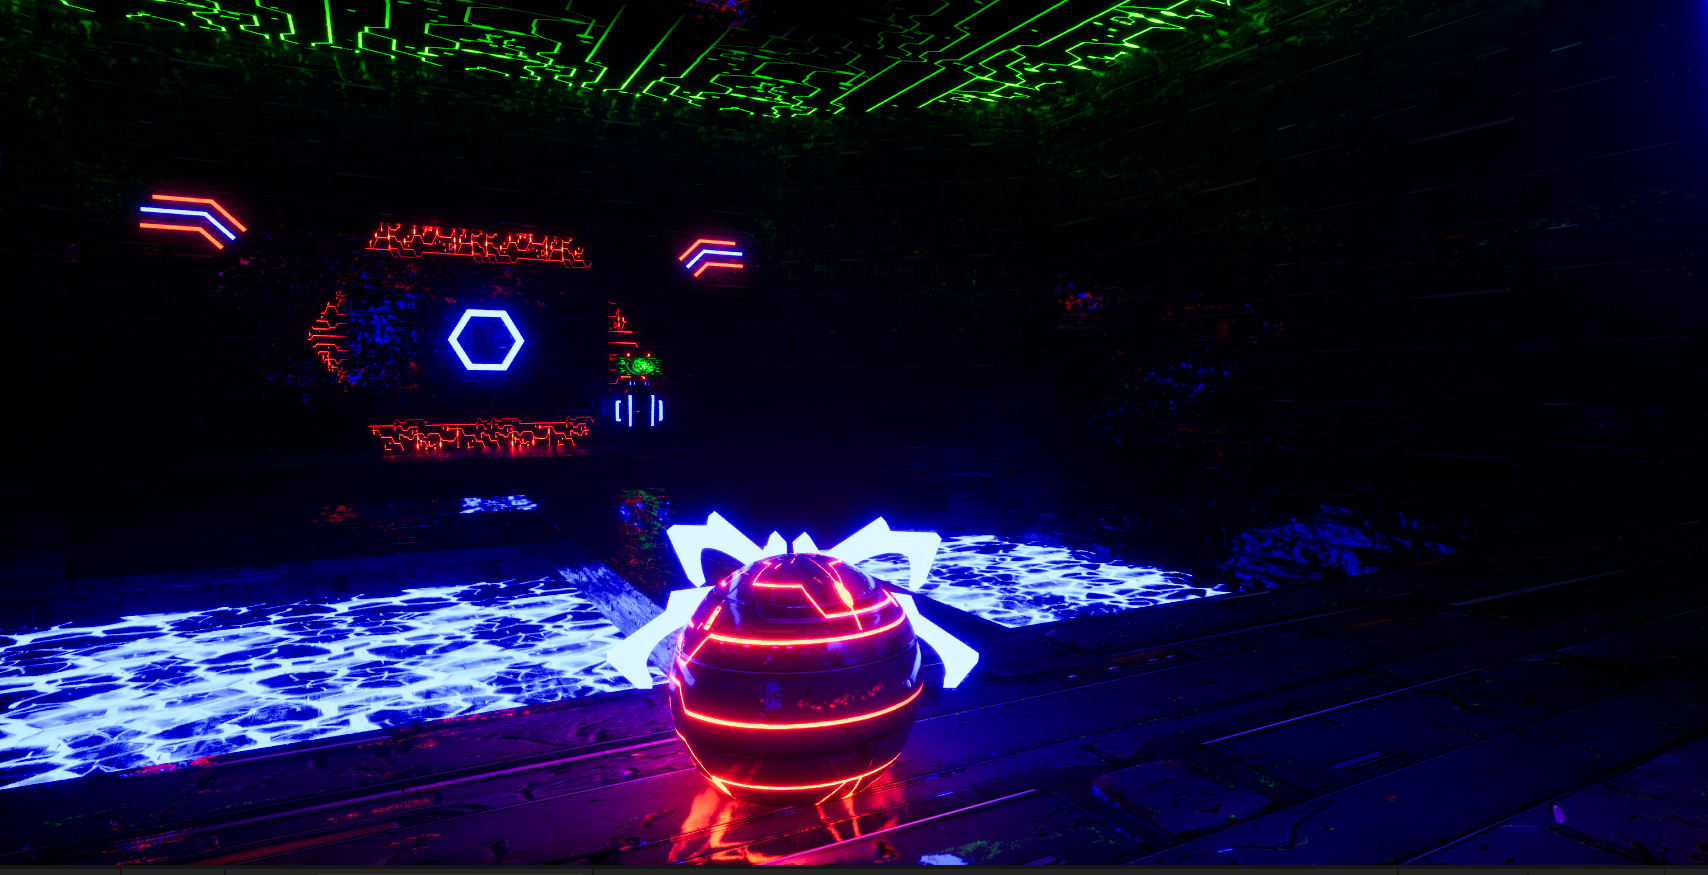
\includegraphics[width=5in,height=2.8in]{MyThesisImages/media/Agent Level 3.png}
    \caption{ Screenshot 3 taken from the UE5 Simulation Environment.}
\end{figure} 
\begin{figure}[H]
	\centering
    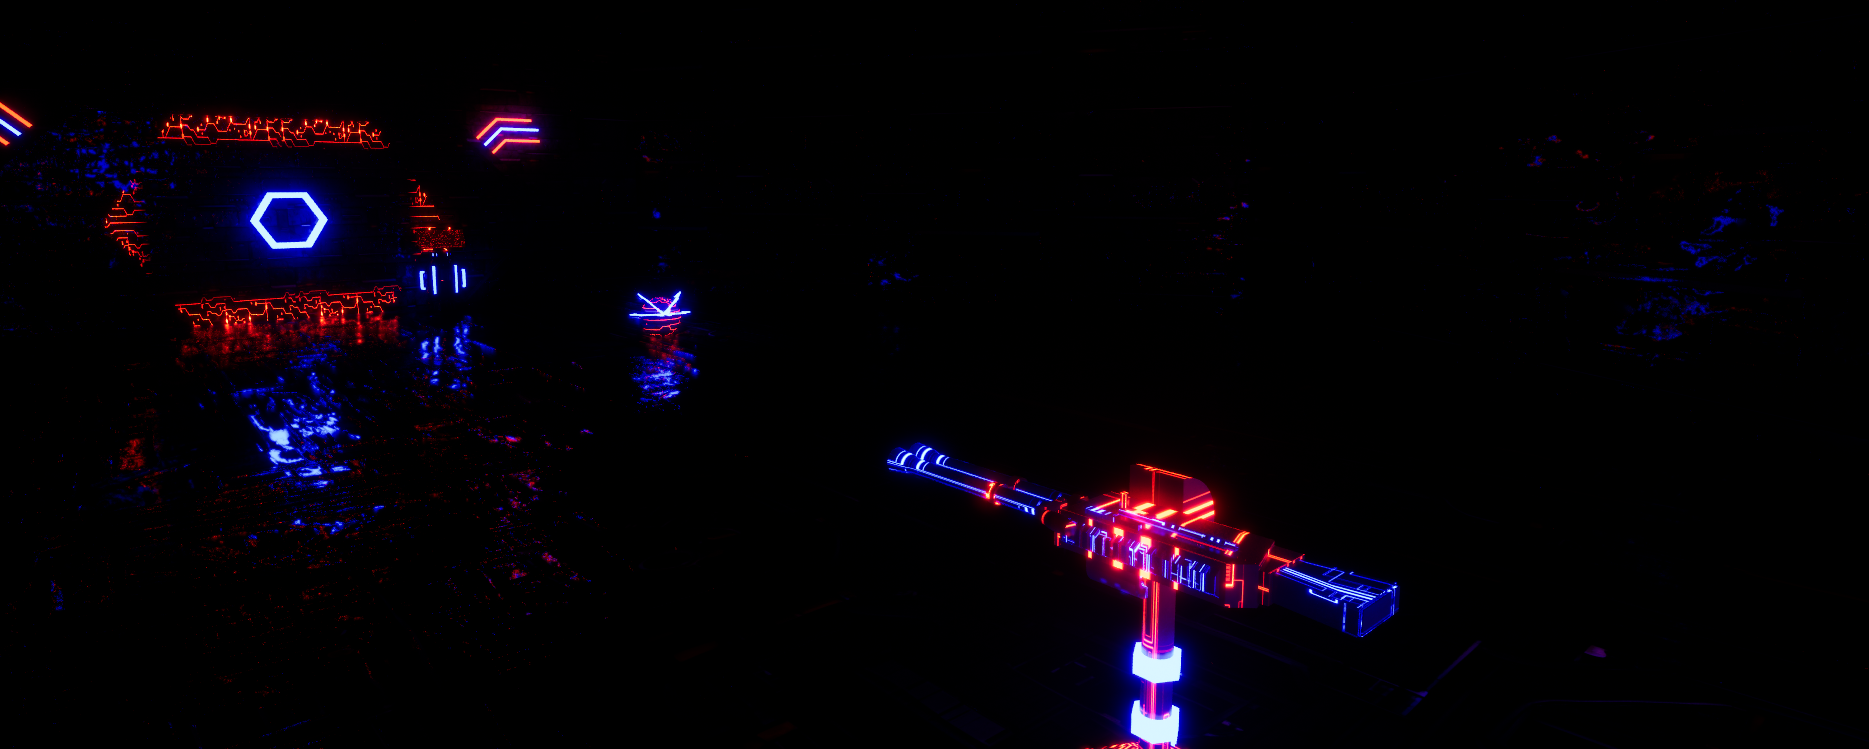
\includegraphics[width=6in,height=3in]{MyThesisImages/media/Agent Level 4.png}
    \caption{ Screenshot 4 taken from the UE5 Simulation Environment.}
\end{figure} 

\subsection{(Section 6.1.c) Designing an Agent}

\begin{figure}[H]
	\centering
    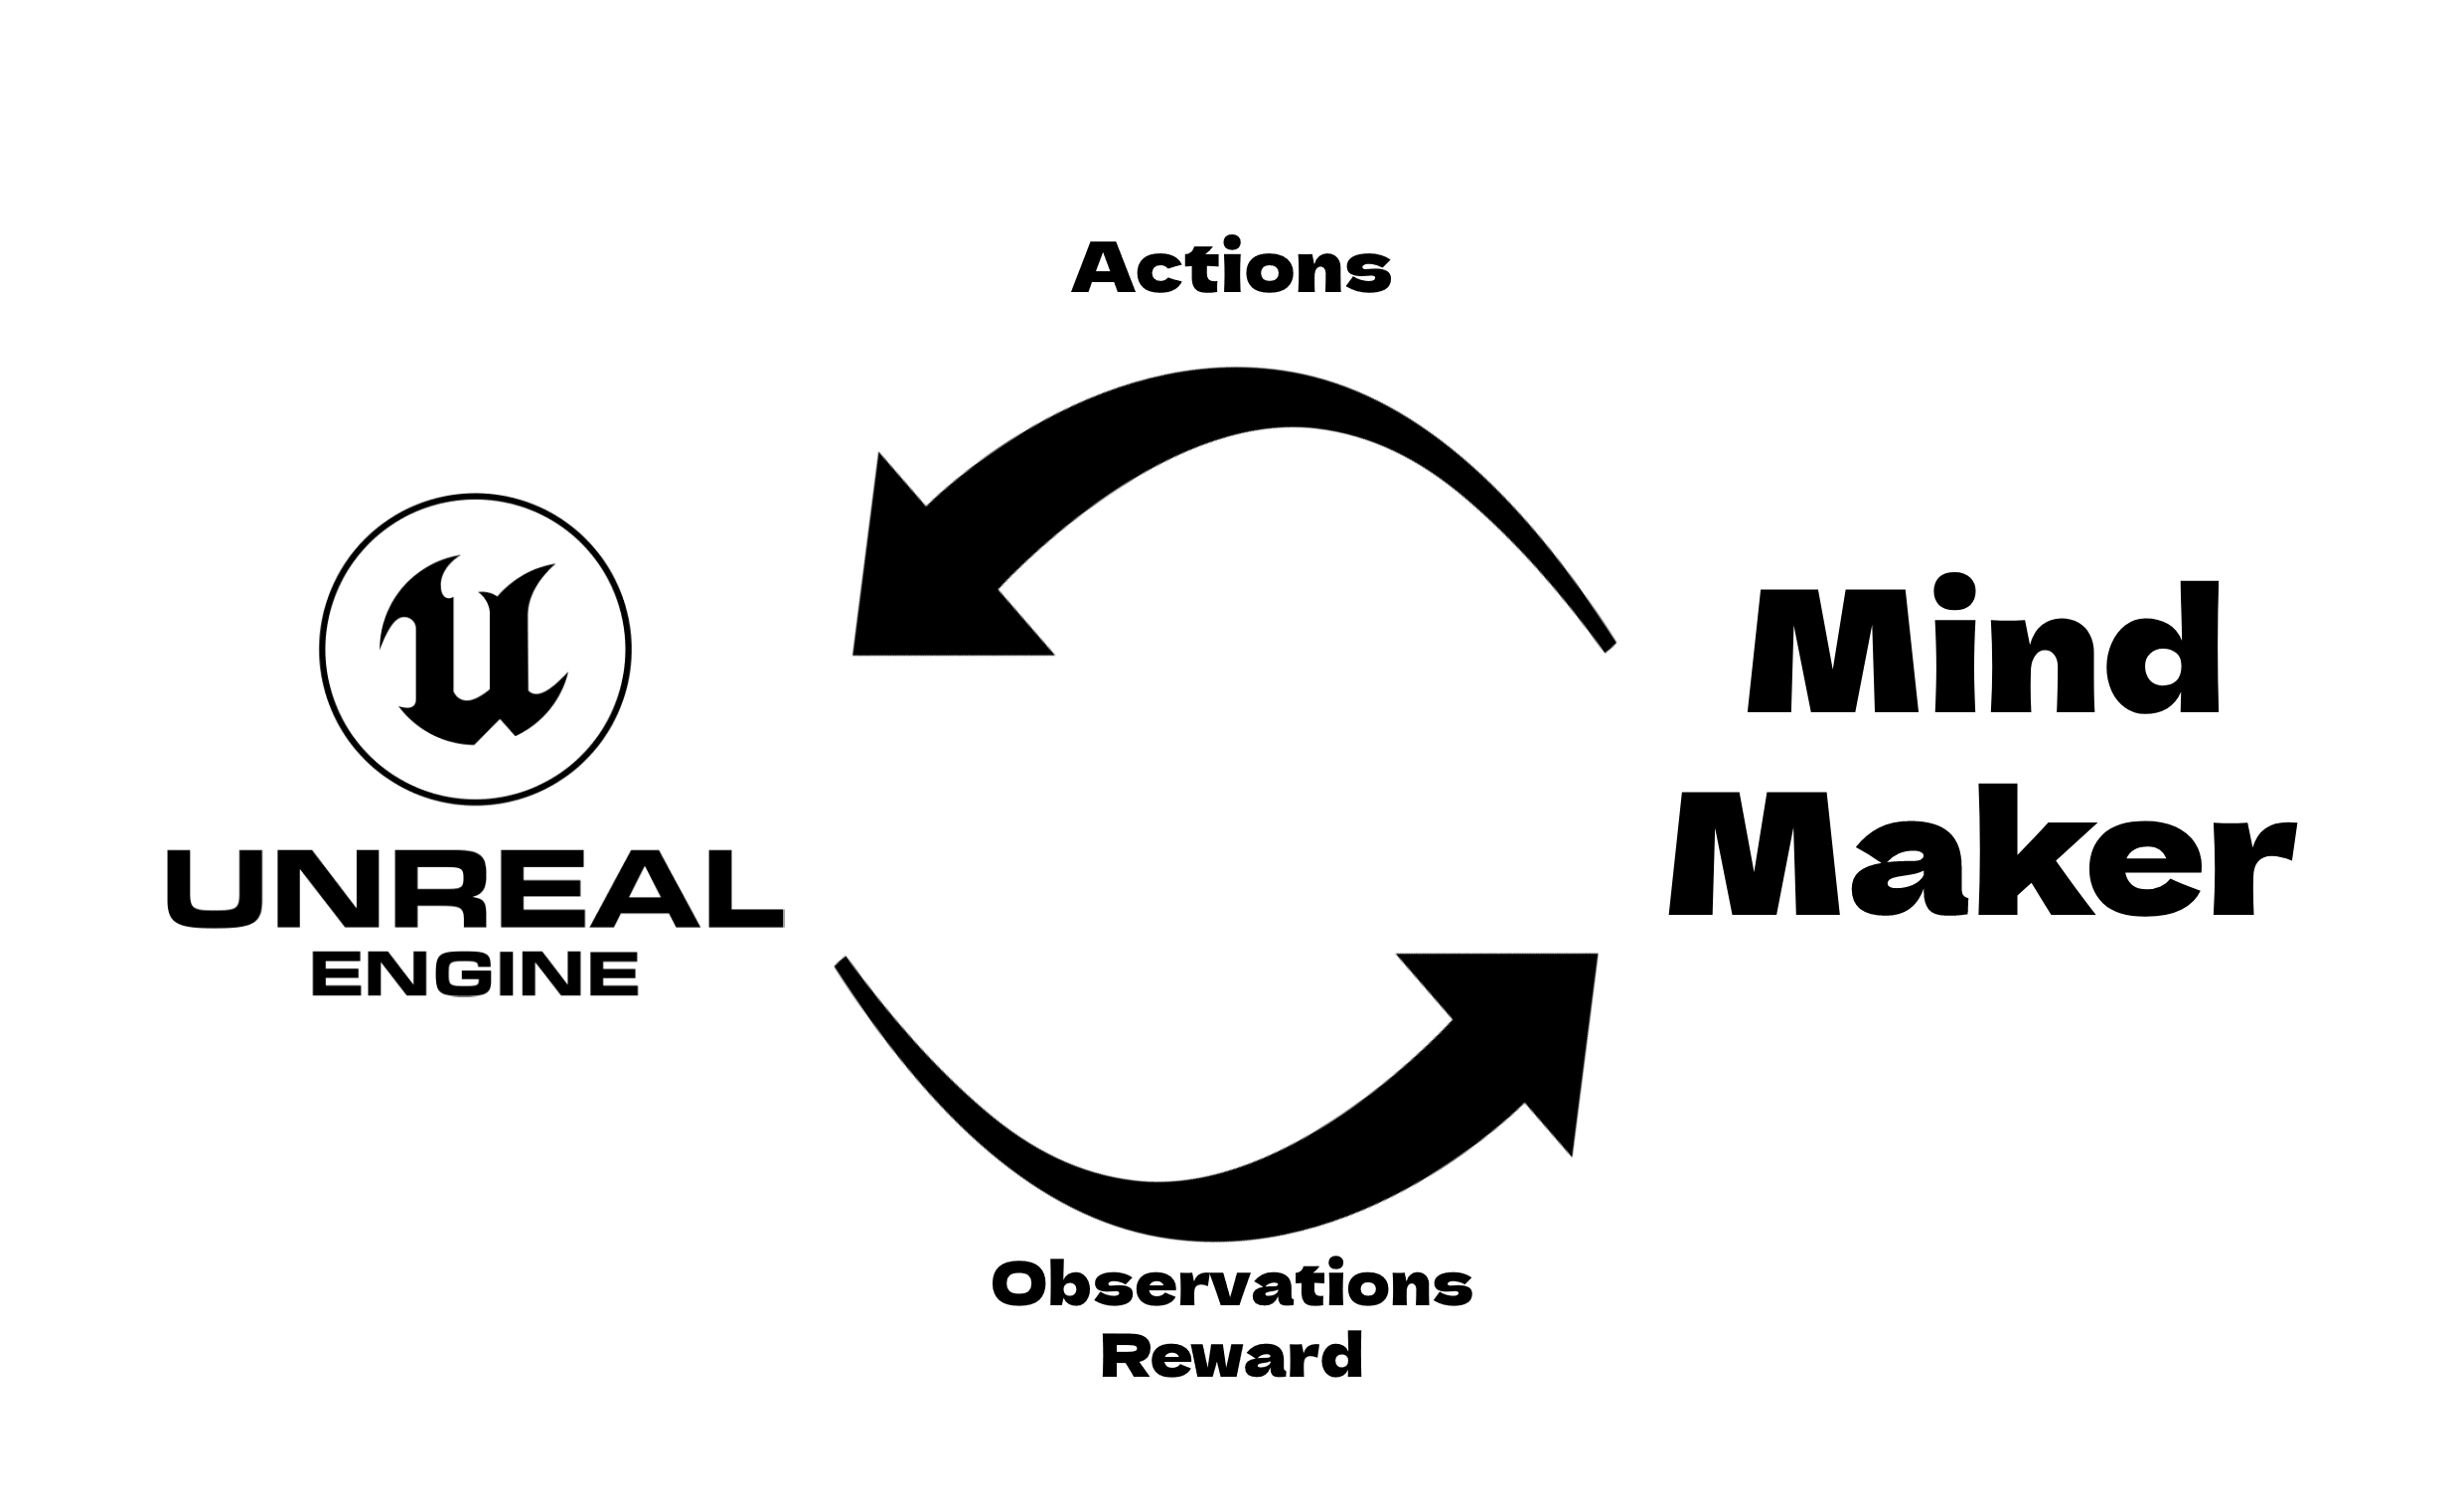
\includegraphics[width=6in,height=3in]{MyThesisImages/media/image124.png}
    \caption{Agent training loop within the unreal engine environment.}
\end{figure} 


As Mind Maker is based on Open AI's Gym python library it uses the same standardized input format as well as algorithms. The models supported by Mind Maker are Stable Baselines 3 implementations of popular models which include:

\begin{itemize}
\item
  Advantage Actor-Critic(A2C)
\item
  Deep Deterministic Policy Gradient (DDPG)
\item
  Twin Delayed DDPG (TD3)
\item
  Deep Q Network (DQN)
\item
  Proximal Policy Optimization (PPO)
\item
  Soft Actor Critic (SAC)
\end{itemize}

Users can choose to use any of those models for training agents inside
Unreal Engine and also have full blueprint control of each model's
neural network hyperparameters.

Deep RL has three core aspects, actions, observations and a reward. The agent does one or more actions, then observes potential changes made to the environment from the actions taken and lastly a reward is calculated based on if certain conditions, set by the programmer, are met.

On the demo game created for this thesis the actions, observations and
the reward function are way more complex than the simple Atari
simulations.

\textbf{ACTIONS}

The agent's Action Space includes the number of actions the agent can
make as well as their respective value ranges.

\begin{itemize}
\item
  Movement Control: Broken down to two axis horizontal and vertical.
\item
  Camera/Gun Control: Broken down to two axis horizontal and vertical.
\item
  Shoot Action: Binary Value for agent to shoot or not.
\item
  Shield Action: Binary Value for agent to use shield action or not.
\end{itemize}

\textbf{Movement}

The game demo is designed in such a way that the movement input needs to
be two variables that each can take 3 possible values. Horizontal -1 to
go left, 0 to do nothing and 1 to go right, similarly in vertical -1 to
go backwards, 0 to do nothing and 1 to go forward.

\textbf{Camera/Gun}

The two input variables for the camera control also control the gun
orientation, therefor whether the camera is pointing affects where the
gun is aiming. They need to be continuous variables from -1 to 1 but
were limited to -0.6 to 0.6 in order to reduce the camera panning speed.

\textbf{Shoot}

Is a binary variable that controls if the agent should shoot or not. If
it is 1 then it shoots if it is 0 then it does not.

\textbf{Shield}

Similarly to shoot action, shield is a binary variable but the shield
mechanic is implemented differently, more specifically unlike shoot that
is a simulated as a single key press, shield has a toggle mechanic.
Meaning that if the agent chooses 1 then the shield is turned on and to
turn it off the agent must pick 1 again, 0 only means that the shield is
kept to its current state regardless of whether its enabled or not.

\textbf{Action Space limitation and shape}

Due to Mind Maker default implementation having restrictions on the
action and observation space types, only Discrete and Box shapes can be
used, lacking more appropriate Multi-Discrete and Dictionary shapes, the
only option for the agent to take multiple actions is to use Box shape.
Inevitably the action space has become continuous for all 6 variables.

\begin{table}[H]
    \centering  
    \begin{tabular}
    {|m{2.5em}||m{5em}||m{4em}||m{5em}||m{5em}||m{2.5em}||m{2.5em}|}
    \hline
         Action & Movement Horizontal & Movement Vertical	&Camera/Gun Horizontal & Camera/Gun Vertical & Shoot&Shield\\
    \hline    
    \hline       					
Low	&-1	&-1	&-0.6	&-0.6	&0	&0\\
\hline   
High	&1	&1	&0.6	&0.6	&1	&1\\

         \hline
    \end{tabular}
    \caption{The action space and low and high bounds
of each variable.}
\end{table} 

\textbf{OBSERVATIONS}

The agent's Observation space, also known as state, includes all the environment variables
that need to be taken into consideration after a certain set of actions
is performed. Generally as a rule of thumb, every variable that will be
used in the reward calculation must be included in the agent's
observations, but when the agent has multiple objectives and a very complex reward function, some
variables considered for the reward might hinder the training by overwhelmingly increasing the state-space.

Deciding which variables should be part of the observation/state of the agent is of at most importance 
during the problems' modelization. A very common mistake occurs when trying to reward the agent based on past successful
actions, similar to a game's score. On model-free algorithms meaning the agents 
take actions in a probabilistic manner based on the current state/observation of the environment. 
If variables referring to the agents' past are considered when taking an action, it will cause confusion 
in the decision process.\\

\textbf{Simplified example of a decision process:}

Possible action: shoot/not shoot

State: enemy targeted/not targeted, can shoot/can not shoot\\

"if enemy targeted and can shoot if you choose action shoot then expected reward +100"\\

\textbf{Simplified example of a decision process with wrong design:}

Possible action: shoot/not shoot

State: enemy targeted/not targeted, can shoot/can not shoot, enemies killed\\

"if enemy targeted and can shoot and enemies killed equal X, if you choose action shoot then expected reward +100"\\\\

With the correct design, when an agent encounters the state [enemy targeted, can shoot] on a random timestep then he 
will have a high probability to choose to shoot due to past iterations that observed the same state and chose the action shoot resulted in 
a positive reward. On the other hand, in the second example even if the agent has successfully killed
some enemies he will not gain knowledge based on the previous experiences because each time the state will be different as the kill count will increase.

When it is needed to reward the agent for performing a desired action we can keep a local variable in the reward function to 
give rewards but not include it in the state, thus resulting in an increased probability of selecting that action when encountering this state.


\textbf{The observation space can include:}\\

\textbf{Combat State}

Binary variable that shows if Agent is in combat or not. The agent
constantly senses if it has enemies in line of sight and sets it to 1 if
enemies found and to 0 otherwise.

\textbf{Can shoot}

Binary variable to control shooting interval after each shot. The agent
makes actions a lot of times per second, this variable is used to deter
him from spamming the shoot action constantly.

\textbf{Hit to Enemy Distance}

Real variable to control how good or bad the agent's aim is. Constantly
a calculation is made for predicting the projectile trajectory if a
bullet is fired in that moment, also when the agent's state becomes 1,
meaning its in combat, the closest in line-of-sight enemy becomes the
currently focused enemy. Hit to Enemy Distance variable is the Euclidean
distance between the predicted hit location and the focused enemy
location.

\textbf{Enemy Targeted}

Binary variable that shows if an enemy is on target. When calculating
the projectile trajectory, we can get access to the item the projectile
will collide with, thus we check if the said item is an enemy and set
the Enemy Targeted Variable to 1.

\textbf{Health Points}

Variable that shows how much damage the agent can take from enemies.

\textbf{Bullet Points}

Variable that shows how many bullets the agent has remaining.

\textbf{Shield Energy Points}

Variable to show the damage the agent can block with shield.

\textbf{Can use Shield}

Binary variable to deter agent from spamming the shield action. Works
similar to "Can Shoot" variable.

\textbf{Coordinate}

Every object has a vector representing its coordinates in the 3D space, 
xyz can be included separately in the Observation or a subset of them if one does not change during playing.

\textbf{Goal Distance}

Real variable to keep track of the agent's distance from the current\\

\textbf{VARIABLES TO AVOID:}\\

\textbf{Hits on Target}

Variable that shows the agent's successful hits on enemies. When an
agent shot projectile inflicts damage to an enemy it rises the count of
the hits on target variable.

\textbf{Kill Count}

Variable that shows how many enemies the agent killed. When an enemy
dies it rises the count of the kill count variable.


\begin{table}[H]
    \centering  
    \begin{tabular}
    {|m{4em}||m{3em}||m{3em}|}
    \hline
         Variable & Low & High\\
    \hline    
    \hline
         State & 0 & 1\\
         \hline
         Can Shoot& 0 & 1\\
         \hline
         Hit-to-Enemy Distance& 0 & 999999\\
         \hline
         Enemy \newline Targeted& 0 & 1\\
         \hline
         Bullet Points& 0 & 100\\
         \hline
         Shield Points& 0 & 50\\
         \hline
         Can Shield& 0 & 1\\
         \hline
        Goal \newline Distance & 0 & 999999\\
         \hline
    \end{tabular}
    \caption{The observation space as well as low and high
bounds of each variable. Some variables have no actual upper bound, arbitrary 999999 value is set.}
\end{table} 

\textbf{REWARD}

After the agent performs the chosen action and makes observations of the
changes to the game environment variables, the last thing to do is to
see if the actions resulted in positive or negative outcomes by running
the reward function to calculate the reward received for those actions.

The Reward function is of at most importance as it steers the agent's
behavior towards the designer's expectations. By setting
action-observation conditions for the agent to meet, the designer can
reward or punish the agent based on the desired behavior he wants him
to achieve.

When designing a reward function careful consideration must be given on
detecting and avoiding trapping states that can steer the agent in
behavior in which he can maximize rewards without progressing towards a
desired objective.

\textbf{Reward Types}

There are many types of methods to give rewards to an agent but in this
implementation the focus will be on dense and sparse rewards.

Using dense rewards means that the agent will be rewarded positively or
negatively according to a set of conditions in each timestep. On the
other hand, sparse rewards are given when an agent completes an
objective.

In this custom designed reward function a combination of sparse and
dense rewards will be implemented to fulfill the different types of
behavior desired. Dense rewards will be used for the main movement and
aiming and sparse rewards for finetuning combat behavior such as
successful hits on an enemy.

\textbf{Reward Conditions}

Following a rigorous design process as well as a lot of trial and error,
the reward function to be used for training the demo agent can
include one or more of these conditions:

\begin{itemize}
\item
  Punishment on health damage/ reward collecting health orbs, equal to
  the health lost or restored respectively.
\item
  Punishment on shield damage/ reward on regenerating shield, equal to
  half of the shield points lost or regenerated to encourage the agent
  to take damage to shield instead to health.
\item
  Punishment on continuous shield spamming.
\item
  Punishment on out of combat shooting.
\item
  Punishment on out of combat use of shield
\item
  Punishment on wrong shoot timing, deter shoot spamming during
  intervals.
\item
  Punishment on shield spamming during shield turns on or off.
\item
  Reward correct shoot timing when enemy is targeted.
\item
  Reward on aiming improvement.
\item
  Reward heading towards the current goal location.
\item 
  Reward reaching the goal line.
\end{itemize}

Due to the limitation of the Mind Maker plug-in for multiple actions to
Box shape which only supports continuous variables we need a way to choose only between the desired actions. 
To achieve that we round the input action variable before the agent makes the action inside the simulation environment.

\begin{itemize}
\item
  Round Movement horizontal to -1 if input action [-1,-0.3), round to 0.0 when [-0.3,0.3) and round to 1.0 when [0.3,1].
\item
  Round Movement vertical to -1 if input action [-1,-0.3), round to 0.0 when [-0.3,0.3) and round to 1.0 when [0.3,1].
\item
  Round action shoot to 0 when input action is [0,0.5) and to 1 when [0.5,1].
\item
  Round action shoot to 0 when input action is [0,0.5) and to 1 when [0.5,1].
\end{itemize}

Pseudocode representing the reward function based on the conditions
listed above:

\begin{minted}{python}

#punish health damage

Reward = Reward + health_points - previous_health_points
previous_health_points = health_points

#punish shield damage

Reward = Reward + (shield_energy_points - previous_shield_energy_points)
previous_shield_energy_points = shield_energy_points

#punish shield spamming

if can_use_shield == 0 and_action_shield == 1:
    Reward = Reward - 1

#punish shoot spamming

if can_shoot == 0 and action_shoot == 1:
    Reward = Reward - 1

if combat state==0 # exploring

#reward heading to goal (punishment on moving away)

    if previous_goal_distance - goal_distance< 0
        Reward = Reward + (previous_goal_distance - goal_distance)
    else:
        Reward = Reward + (previous_goal_distance - goal_distance)
        previous_goal_distance = goal_distance

#punish out of combat shooting

    if action_shoot == 1:
        Reward = Reward - 100

#punish out of combat use of shield

    if action_shield == 1:
        Reward = Reward - 100

elif combat state == 1: # combat

#reward aiming improvement

    if enemy_targeted == 0:
        Reward = Reward +
            (previous_hit_to_enemy_distance - hit_to_enemy_distance)
        previous_hit_to_enemy_distance = hit_to_enemy_distance

#punish shooting when enemy not targeted

        if action_shoot == 1:
        Reward = Reward - 100

#reward shoot when enemy targeted

    elif enemy_targeted==1:

        If can_shoot==1 and action_shoot==1
            Reward = Reward + 50
\end{minted}

\textbf{Training Environment}

Most DRL agent training simulations from Open AI Gym are done on a
single level with only one objective, "get on top of the hill", "land
the spaceship upright", "balance the pendulum" etc. To train the
agent in this demo game is magnitudes more difficult in terms of
complexity as the agent has multiple mechanics to be trained on:

\begin{itemize}
\item
  Finetune controls
\item
  Path finding
\item
  Aiming
\item
  Shooting
\item
  Avoiding damage
\end{itemize}

That's why the training level was designed in distinct rooms which step
by step guide the agent to the next goal. The agent will be trained in a
level specifically designed towards an incrementally increasing
difficulty in both exploration and combat scenarios. It will include six
different rooms each one with a specific training objective in order to
steer the agent to a desired behavior.

\textbf{Goals}

\begin{enumerate}
\def\labelenumi{\arabic{enumi}.}
\item
  Enter room 1.
\end{enumerate}

\begin{enumerate}
\def\labelenumi{\arabic{enumi}.}
\item
  Find path and enter room 2.
\item
  Find path between lasers to collect battery from room 3.
\item
  Go back to room 2 and unlock the door with the collected battery.
\item
  Go to room 5 after fight in room 4.
\item
  Go to room 6 after pathfinding in room 5, with intentional local maxima path.
\item 
  Go to last goal by climbing a ramp with incline.
\end{enumerate}

\textbf{Starting Room}

The room in which the agent is spawned in the beginning of the training.
Goal 1 is to go from the starting room to Room 1, there are no
obstacles, and the objective is for the agent to learn the basic
controls as well as to head towards a specific goal location.

\textbf{Room 1}

In this room the target is for the agent to learn how to navigate and
find a path to reach the second room. Two possible paths are given as
bridges that allow the agent to cross the gap.

\textbf{Room 2}

A transition type of room with a locked door that the agent needs to go
to a different room to find the key. It doesn't introduce a new
objective as the agent only sees a goal location and doesn't have
understanding of the locked door mechanic, it is a harder variation of
the previous room that the agent needs to navigate in order to go to
Room 3.

\textbf{Room 3}

This room has the key for the locked door (Battery), that is protected
by an array of lasers. The agent needs to find the correct path between
the lasers that inflict contact damage to his health points each second.
The agent in this room could learn punishment mitigation with the use of
the shield and ultimately find the path which will result in him not
taking damage.

\textbf{Room 4}

First contact with a stationary enemy turret. Agent must defeat the
enemy to progress to the next goal. Objective is learning how to aim,
shoot, avoid enemy hits and use shield. The agent gets a handicap at the
beginning to not overwhelm him, the turret is deactivated for the first
5 times the room is repeated, so the agent can learn to correctly aim
the gun, afterwards the enemy starts shooting projectiles at the agent.

\textbf{Room 5}

Same bridge navigation type of level but with an introduced path that
doesn't reach the other side. A purposely introduced local maxima for
the agent to learn to navigate out of.

\textbf{Room 6}

The final room is an advanced combat room, the room includes a new type of enemy a laser turret, which has more health points and does contact
damage per second.

\textbf{Training Level Completed Room}

After defeating the enemy in room 6, the agent must navigate to the
final room by passing over a low friction ramp which has a big incline.
If the agent does not have the proper velocity at the beginning or if he
loses velocity during the climb, the low friction will not allow him to
proceed and will fall back. To complete the room the agent must reach
the top of the ramp.

\textbf{Training Loop}

Each goal must be completed 10 times before the agent can progress to
the next one. After reaching the final goal the 10th time, the agent
starts the level from the beginning.

\textbf{Training Method}

Due to the complexity of the demo game created, the number of training
steps the agent will need in order to learn the game is unknown. We
couldn't try to make an educated guess just by looking at each
individual problem (path finding, aiming etc.) and sum our prediction to
derive the final number because combining all of them makes the problem
exponentially more difficult.

Due to hardware and time limitations we will implement multiple agents to test each training
objective separately as the goal of the thesis is not to produce a complex agent but to prove the 
simulation capabilities of the unreal engine environment. 

Someone can still design big multi-objective agent to be trained in this environment by combining all the objectives together in a large and complex reward function.

Another useful feature of  the Mind Maker plugin is Saving and Loading Models, which allows us to locally save the trained model and load it for
prediction or more importantly for continuous training which is ideal
for our training application.

\section{(Sub-chapter 6.2) Deep RL Algorithm Chosen for Agent Training}

The MindMaker tool gives us access to many different algorithms to use for training 
Agents, between all the available ones Proximal Policy Optimization-PPO was chosen due to 
its compatibility with the training objectives and capability of handling continues variable types.


\textbf{Characteristics of PPO:}

\begin{itemize}
\item
  Model-free
\item
  Gradient based
\item 
  On-Policy
\item
  Actor-Critic
\item
  Policy Clipping
\end{itemize}


\textbf{The basic idea behind PPO:}
\begin{itemize}
  \item
    The \textbf{actor} calculates a probability distribution for the next action the agent should take based on the current state/observation.
  \item
    The \textbf{critic} estimates an expected cumulative reward based on the current state/observation.
  \end{itemize}

The goal of PPO is for the actor to choose actions which will be more likely to result in a higher reward than expected by the critic.
In order to achieve that, a metric value called "Advantage" is used in the algorithm, which measures how wrong the critic estimation was for any given state.
If the advantage is negative then the action resulted in a lower cumulative reward than the critic expected thus we make that action have a lower probability of being chosen.
On the other hand if the estimated advantage is positive then it means that the action resulted in a higher reward than expected, thus we make it have a higher probability of being chosen.

To have good advantage estimation, a critic that can predict as accurately as possible the value of any given state. 
The Mean Square Error of the estimated and the observed cumulative rewards is implemented as the critic's loss function.

\textbf{PPO training loop:}
\begin{minted}{python}
  int iterations= Training_episodes / N_steps
  for iteration in range(iterations):
    for actor in range(x):
      #Run policy for N_steps
      #calculate advantage for each step
    
    #Update policy

\end{minted}


\section{(Sub-chapter 6.3) Experiments, Training Results and Observations}

In this section the results of the agent training inside the unreal
engine will be presented. The MindMaker plugin allows for saving
tensorboard logs after each training session.

All the experimental agents will be designed and trained using the Proximal Policy Optimization
(PPO) algorithm using continuous training method discussed previously.

The hyperparameters of the algorithm will be kept the same for each of the experiments for simplicity and 
to assure a degree of consistency between all the agents, even if they might be not optimal for all scenarios.
\begin{longtable} 
{|m{7em}||m{7em}|}
    \hline
        Policy & MlpPolicy \\
        \hline
        Learning rate	&0.00025\\\hline
        N steps	&2048\\\hline
        Batch size&	32\\\hline
        N epochs	&4\\\hline
        Gamma	&0.99\\\hline
        Gae lambda&	0.0\\\hline
        Clip range	&0.2\\\hline
        Clip range vf	&None\\\hline
        Normalize advantage&	False\\\hline
        Ent coef	&0.01\\\hline
        Vf coef&	0.5\\\hline
        Max grad norm&	0.5\\\hline
        Use sde	&False\\\hline
        Sde sample freq&	0\\\hline
        Target kl	&None \\\hline
        Tensorboard log&	Filepath\\\hline
        Create eval env	&False\\\hline
        Verbose	&1\\\hline
        Seed	&0\\\hline
        Device	&Auto\\\hline
        Init setup model&	True\\\hline
        Activation function&	Th.nn.Tanh\\\hline
        Network arch&	[512,512]\\\hline

        
         \caption{Custom hyperparameters used for the PPO algorithm.}
\end{longtable}

Due to technical challenges and hardware unavailability, we ended up breaking up the multi-objective reward function 
and focus on training multiple smaller agents experimentally. The setup is a personal computer with an 
 i5 10400f CPU, 16gb ram and 3060ti GPU, which is not nearly capable of achieving 
 significant results in a realistic time frame. Nevertheless, these experimental 
 attempts showcase greatly the DRL simulation capabilities of a game development environment such as unreal engine. 

\subsection{(Section 6.3.a) Experiment 1- Movement and camera control}

The first experiment will call for the agent to handle 4 different inputs for movement and camera control
as they  were designed as a linked system in the demo game. The axis for the ball movement are not static with the world 
but are rotating based on the camera's forward vector, that means that forward is where the camera is facing at.  

\begin{figure}[H]
	\centering
    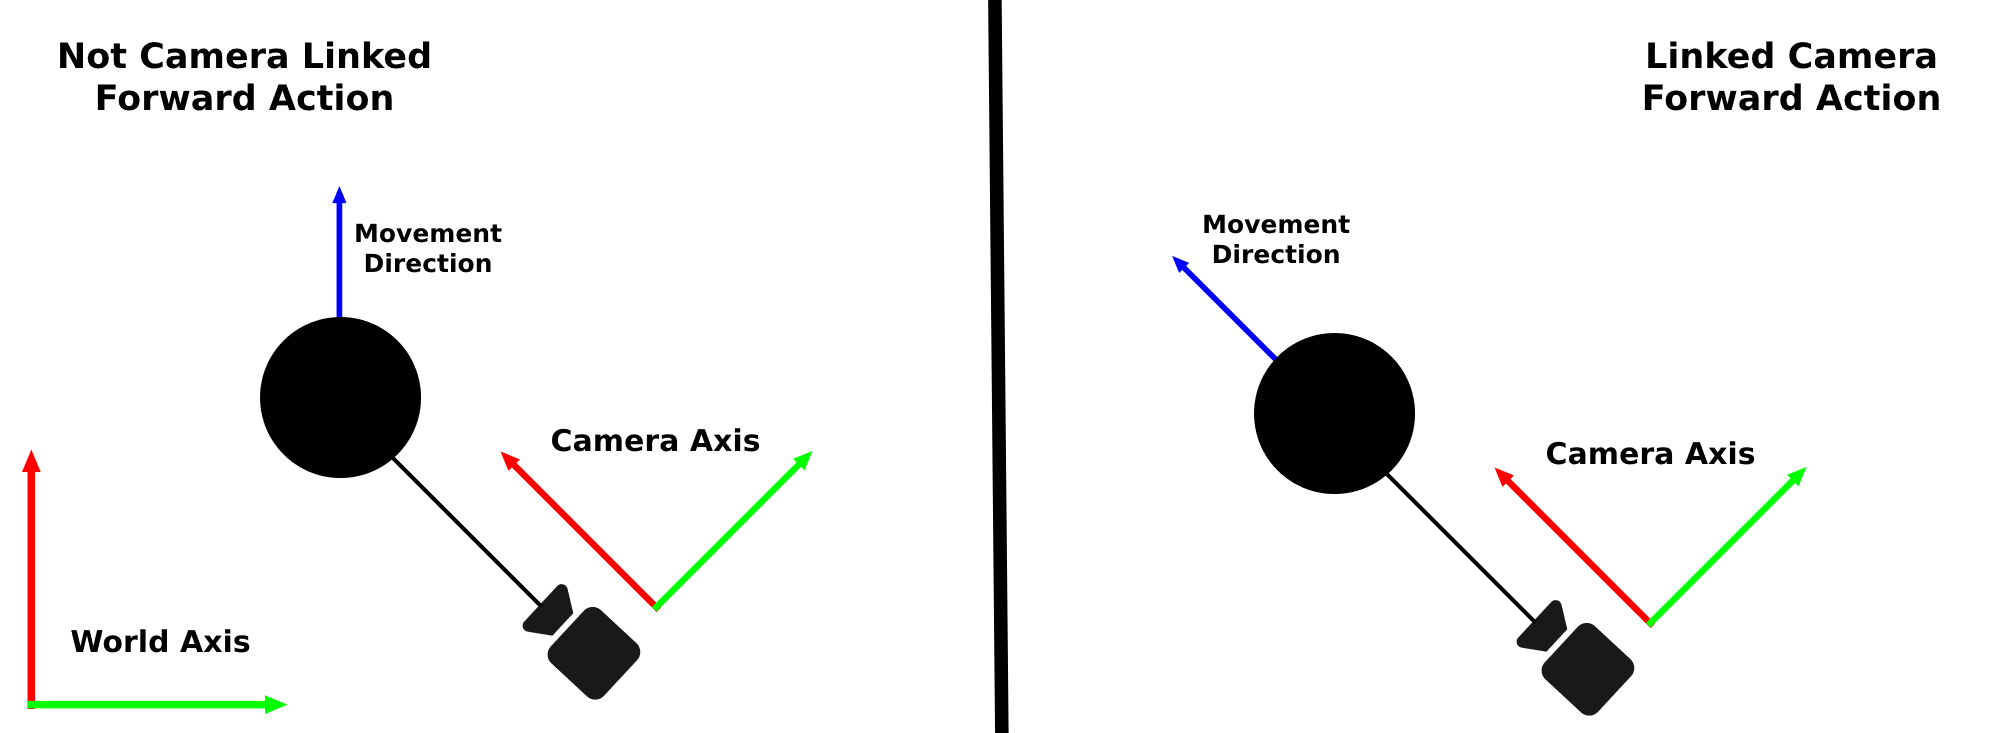
\includegraphics[width=6.25764in,height=2in]{MyThesisImages/media/linked camera movement comparison.png}
    \caption{Demonstration of the movement-camera linked system.}
\end{figure}

\begin{table}[H]
  \centering  
  \begin{tabular}
  {|m{2.5em}||m{5.2em}||m{4em}||m{6em}||m{6.5em}|}
  \hline
       Action & Movement Horizontal & Movement Vertical	&Camera/Gun Horizontal & Camera/Gun Vertical\\
  \hline    
  \hline       					
Low	&-1(backwards)	&-1(left)	&-0.6(look left)	&-0.6(Look down)\\
\hline   
High	&1(forwards)	&1(right)	&0.6(look right)	&0.6(look up)\\

       \hline
  \end{tabular}
  \caption{Experiment 1 action space and low and high bounds
of each variable.}
\end{table} 

The observation space will only be the Euclidean Distance between the agent's location and goal location.
\begin{table}[H]
  \centering  
  \begin{tabular}
  {|m{5em}||m{5em}|}
  \hline
       Observation & Distance\newline to goal\newline location\\
  \hline    
  \hline       					
Low	&0\\
\hline   
High &10000\\

       \hline
  \end{tabular}
  \caption{Experiment 1 observation space/ State with low and high bounds.}
\end{table} 

Reward function that the agent will try to maximize:

\begin{minted}{python}
float previews_goal_distance=goal_distance #initialize in the first step

#in each step calculate the reward

if previous_goal_distance - goal_distance< 0
  Reward = Reward + (previous_goal_distance - goal_distance)*x
else:
  Reward = Reward + (previous_goal_distance - goal_distance)

previous_goal_distance = goal_distance
\end{minted}


In this reward function the objective is to get a positive outcome from the 
previous goal distance minus the current goal distance, that will only occur when the agent selects an action
that will make the current goal distance smaller in each step which will make him head towards the goal location. 
The x variable is a multiplier for the negative reward, in this case it was kept at 1 and does not interfere, 
but it can be made larger to increase the negative reward when moving away from the objective.

An important observation in this first experiment is that the agent was very confused in certain spots in the room,
it was determined that the agent is sensitive in distance symmetric positions. Due to the fact that the agent has only a 
distance observation, he makes associations between distance measurements and actions that will result in a higher expected reward, 
but if the same state can be observed in two or more  different locations in the level it results in a confused agent.

\begin{figure}[H]
	\centering
    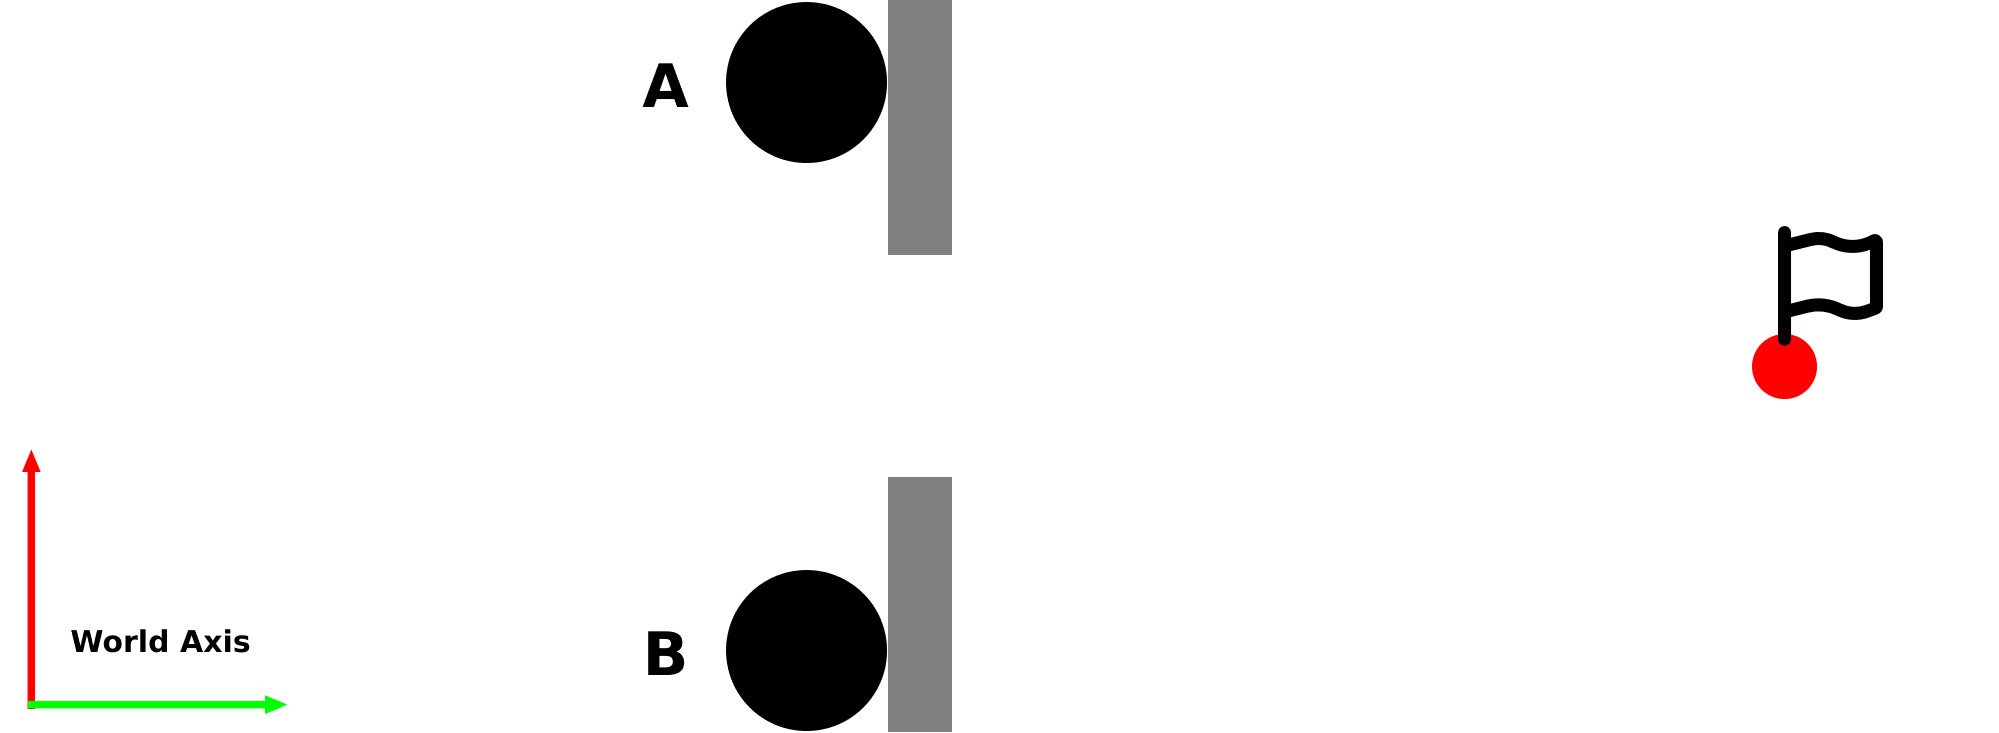
\includegraphics[width=4in,height=1.5in]{MyThesisImages/media/DISTANCE PROBLEM.png}
    \caption{The symmetric distance problem. A and B are the same distance away from the goal but in different locations}
\end{figure}


\subsection{(Section 6.3.b) Experiment 2- Improved Movement and camera control}

The second experiment will try to clear the confusion in the agent's decision selection by 
incorporating the x and y coordinates (z does not change so it was not included) in order to create distinct action-Observation associations 
based on the agent's current location as well as distance from the goal.

Another important problem the agent faces is the linked camera-movement system, meaning that the camera rotation around the
z axis affects the result of any given agent movement action. as demonstrated by the figure below the agent can be on state with 
the same distance, identical xy coordinates but depending on the camera rotation the input action will result in a different outcome.

\begin{figure}[H]
	\centering
    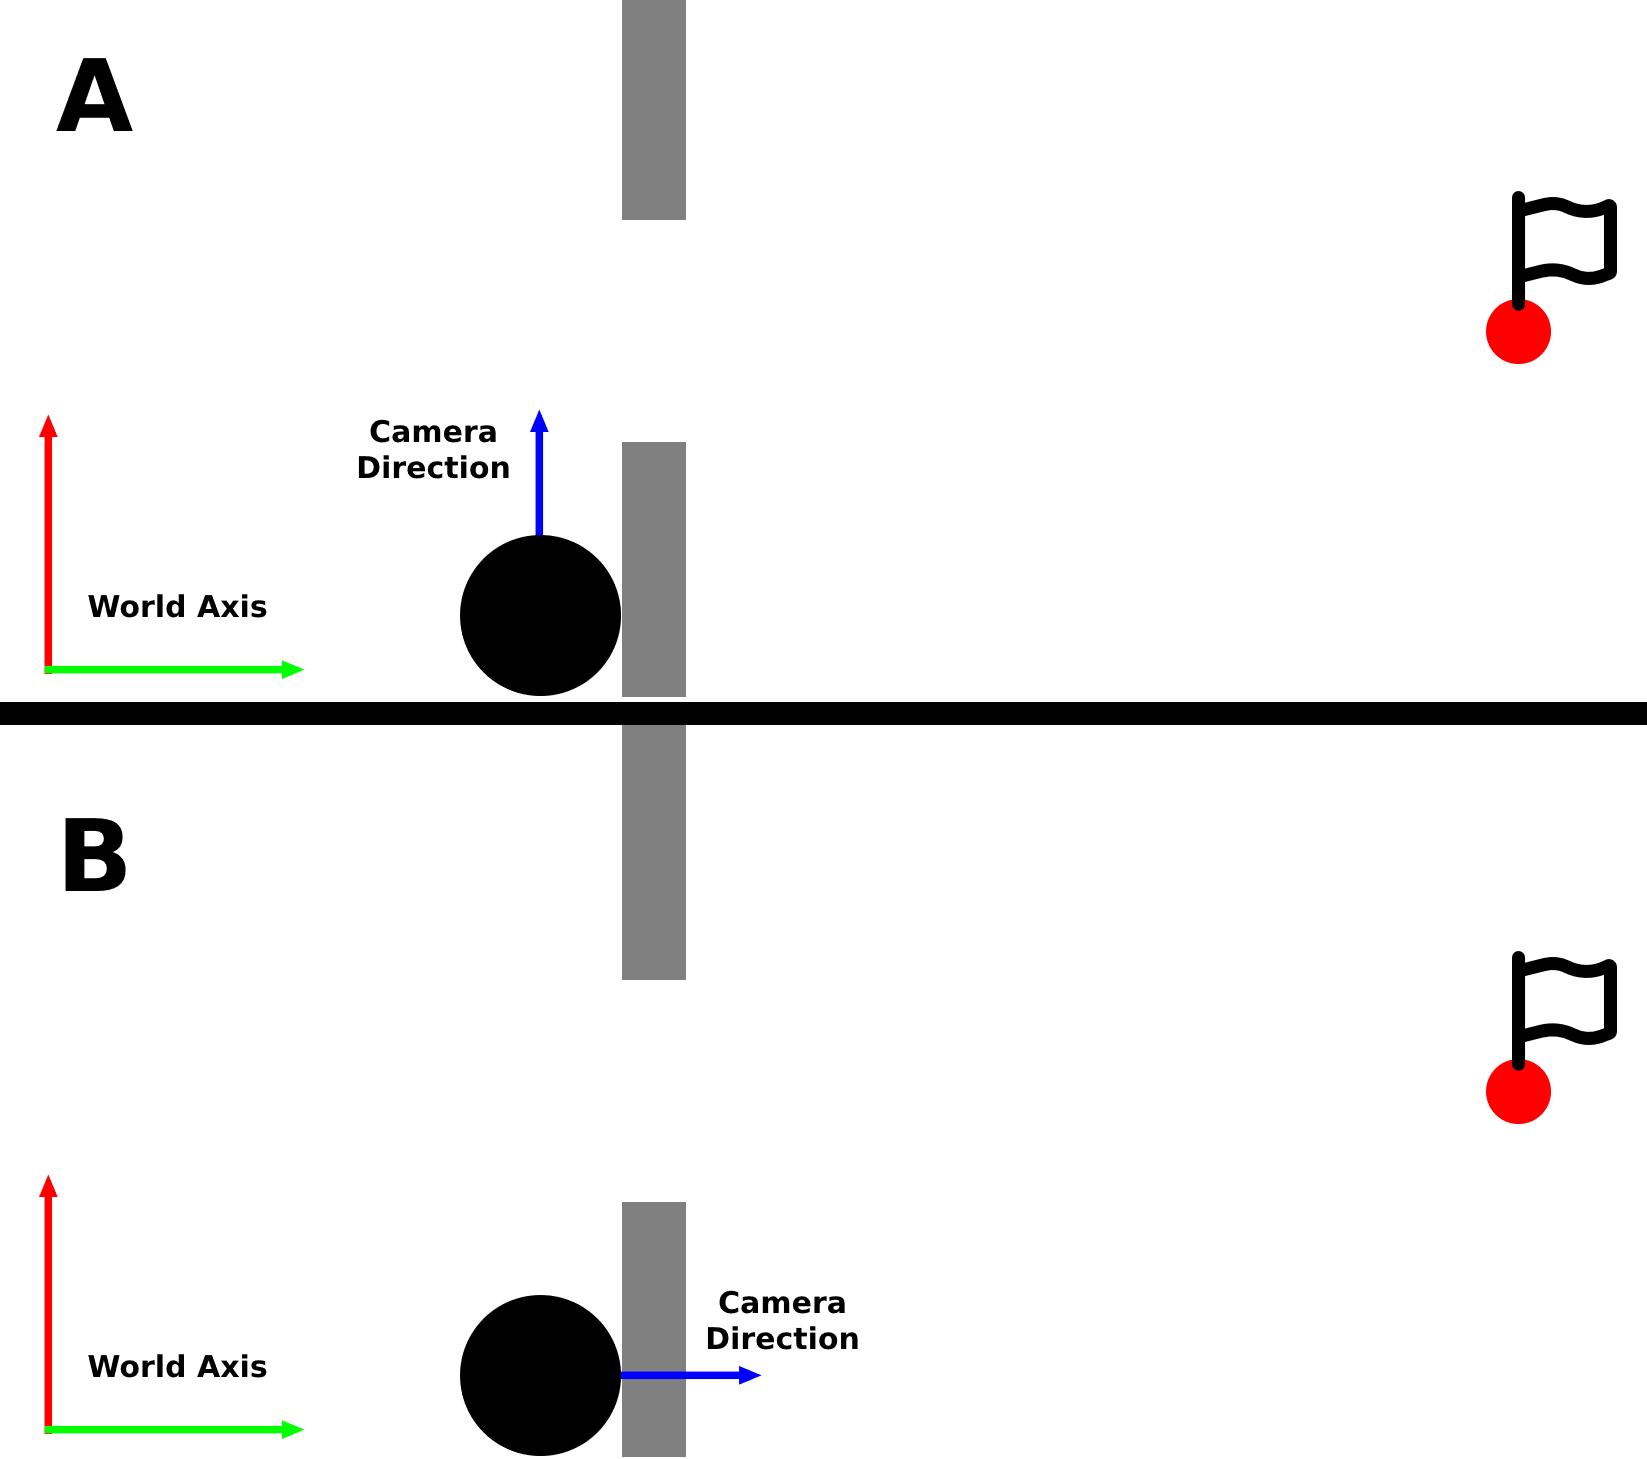
\includegraphics[width=4in,height=3.5in]{MyThesisImages/media/CAMERA ROTATION PROBLEM.png}
    \caption{ The camera Z rotation problem. A and B are in the same location but have different camera Z rotation}
\end{figure}

In example A from the figure above a sideways left action will result in a negative reward as the agent will increase the distance from the goal,
on the other hand the same action will produce a favorable out come in the example state B. It is necessary to include the camera z rotation in order
to help the agent select the correct action for each circumstance.

The action space will remain the same as the first experiment, but the observation space will change as follows.

\begin{table}[H]
  \centering  
  \begin{tabular}
  {|m{5em}||m{3.5em}||m{5em}||m{5em}||m{4em}|}
  \hline
  Observation &Distance\newline to goal\newline location &x coordinate &y coordinate & Camera\newline Z rotation\\
  \hline    
  \hline       					
Low	&0 &-500 &-2500 &-180\\
\hline   
High &10000 &9000 &2500 &180\\

       \hline
  \end{tabular}
  \caption{Experiment 2 observation space/ State with example of low and high bounds.}
\end{table} 

Reward function that the agent will try to maximize will remain the same as the previous experiment,
as the objective does not change, only the observation space is expanded in order to provide
more accurate information to the agent and avoid confusing the algorithm with duplicate states that require 
different actions to be selected.\\

\textbf{Additional improvements:}

After multiple experimental runs of this setup the agent was observed spending too much time stuck on the walls
and especially in the corners of the room, in some cases resulting in the algorithm getting trapped in the corner.
In order to get the agent unstuck from the walls and promote more exploration of the room, two measures were taken:
\begin{itemize}
  \item Adding another face to the hexagon room and making it an octagon, removing the problematic corners
  \item Implementing a "Don't touch the wall" mechanic in the game. If the agent touches the wall he is returned to the starting position 
        and receives a 1000 points punishment to the reward
  \item All Observation variables were rounded to the nearest integer, meaning reducing the location accuracy of the agent to centimeters 
        and the rotation accuracy to non-fractional degrees. This accuracy reduction is negligible compared to the state space reduction it gives us.
\end{itemize}
A huge improvement in the agent's exploration process of the room was observed as well as better "runs" to the desired goal location.


\subsection{(Section 6.3.c) Experiment 3- Stationary Aiming}

The third experiment will focus on training an agent to aim at an enemy. For simplicity, both the agent and the enemy will be
stationary and the enemy will not try to damage the agent. The agent's objective is similar to the movement as he tries to minimize the distance between where he is aiming and the target enemy.
The aiming system is linked with the camera rotation, has 360 degrees of freedom in the horizontal axis but is limited in the vertical axis from 20 to -20 degrees.

\begin{figure}[H]
	\centering
    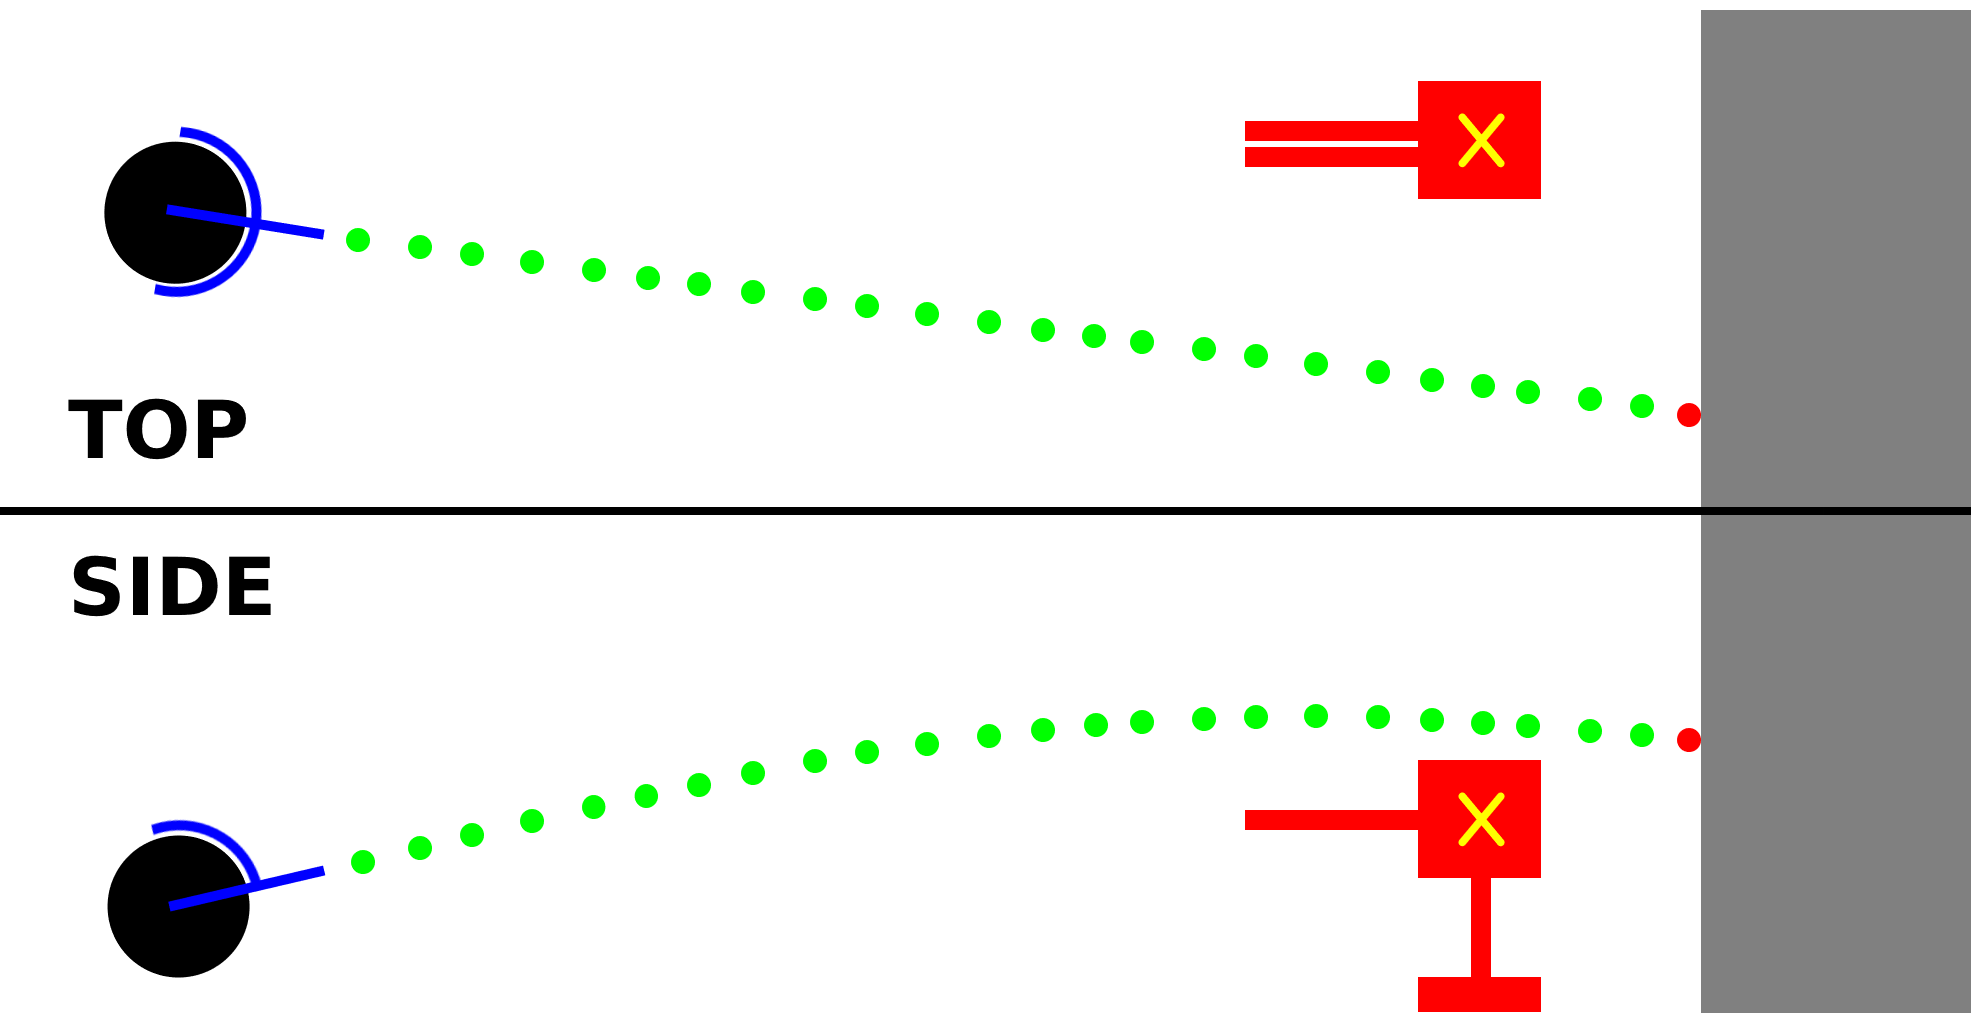
\includegraphics[width=4in,height=2.3in]{MyThesisImages/media/Agent Aim.png}
    \caption{Agent aiming diagram. The red dot represents the predicted hit location and yellow X the target location.}
\end{figure}

At every timestep a calculation of the location that the projectile will make if shot is made and the Euclidean distance between the aimed location and the current enemy's location
is computed. The agent is rewarded for each centimeter he aims closer to the enemy and is punished when that distance becomes larger.

\begin{table}[H]
  \centering  
  \begin{tabular}
  {|m{2.5em}||m{6em}||m{6em}|}
  \hline
       Action &Camera/Gun Horizontal	&Camera/Gun Vertical \\
  \hline    
  \hline       					
Low	&-0.6(look left)	&-0.6(Look down)\\
\hline   
High &0.6(look right)	&0.6(look up)\\

       \hline
  \end{tabular}
  \caption{Experiment 3 action space and low and high bounds
of each variable.}
\end{table} 

The observation space will include the Euclidean Distance between the current aimed location 
and enemy's location, as well as the xyz coordinates for the aimed location.
\begin{table}[H]
  \centering  
  \begin{tabular}
  {|m{5em}||m{3.5em}||m{5em}||m{5em}||m{5em}|}
  \hline
       Observation &Hit to\newline enemy Distance &x coordinate &y coordinate &z coordinate\\
  \hline    
  \hline       					
Low	&0 &15000 &-2500 &-100\\
\hline   
High &10000 &19000 &2500 &1500\\

       \hline
  \end{tabular}
  \caption{Experiment 3 observation space/ State with low and high bounds.}
\end{table} 

Reward function that the agent will try to maximize:

\begin{minted}{python}
float previews_distance=current_distance #initialize in the first step

#in each step calculate the reward
Reward = Reward + (previous_distance - current_distance)
previous_distance = current_distance
\end{minted}


\subsection{(Section 6.3.d) Experiment 4- Stationary Aiming and Shooting}

The fourth experiment will focus on extending the third one by including a shooting mechanic on top of the aiming. The agent's objective is more complex this time as he tries to aim and simultaneously decide when to shoot. 
The agent's action space has a "shoot" action which when chosen a projectile will be fired, this action has a 0.5 second cooldown period, if the agent tries to spam the action during
the cooldown time he is punished.

Another variable the agent takes into consideration is if the enemy is targeted, that is a binary variable that is 0 when the calculated projectile hit location is not on top of the enemy and becomes 1 when 
this location is on the enemy even if it does not match the focused location the agent tries to aim at. If the enemy decides to shoot when the enemy is targeted then he is rewarded. 
The purpose of this variable is to increase the number of states in which the agent can be rewarded for correct shooting.

\begin{table}[H]
  \centering  
  \begin{tabular}
  {|m{2.5em}||m{6em}||m{6em}||m{4em}|}
  \hline
       Action &Camera/Gun Horizontal	&Camera/Gun Vertical & Shoot\\
  \hline    
  \hline       					
Low	&-0.6(look left)	&-0.6(Look down) &0(No shoot)\\
\hline   
High &0.6(look right)	&0.6(look up)&1(shoot)\\

       \hline
  \end{tabular}
  \caption{Experiment 4 action space and low and high bounds
of each variable.}
\end{table} 

The observation space will include be the Euclidean Distance between the current aimed location 
and enemy's location, as well as the xyz coordinates for the aimed location. Additionally a "Can Shoot" variable
for the cooldown between shots and a "enemy targeted" variable to show is enemy is targeted or not at any given observation/state. 
\begin{figure}[H]
	\centering
    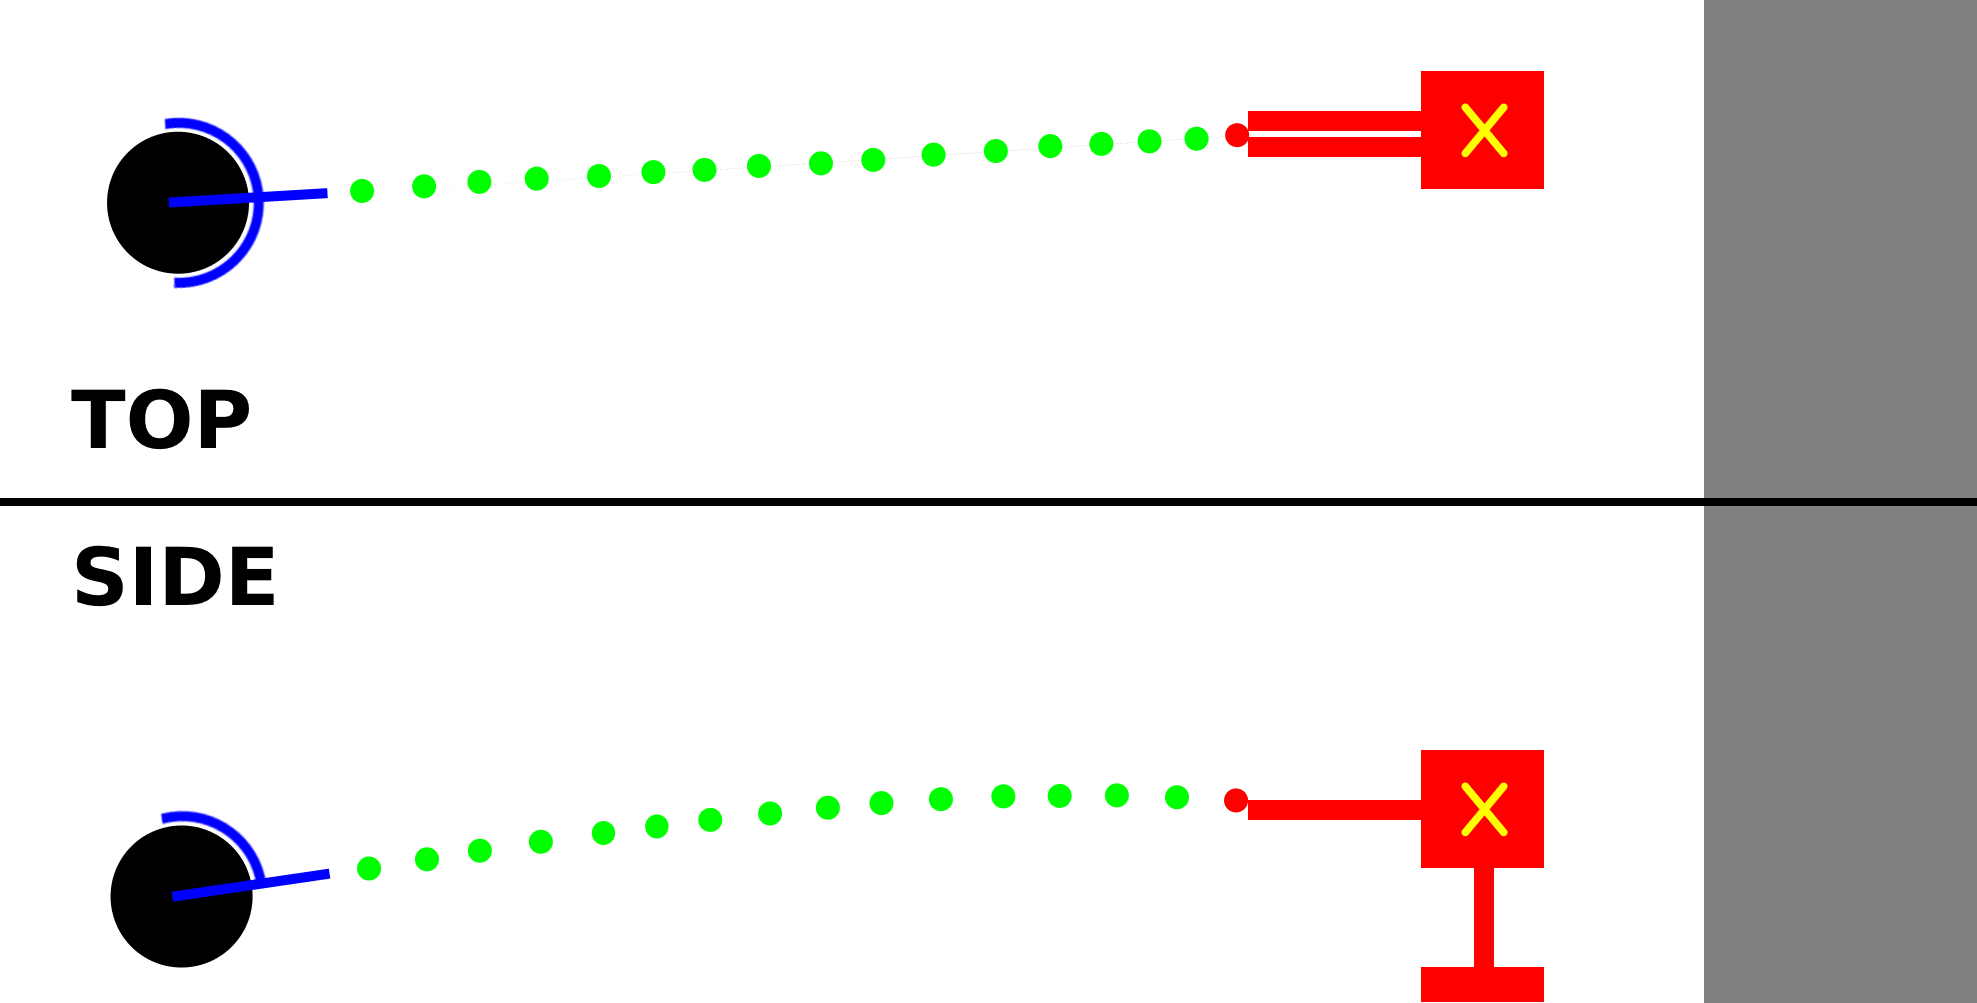
\includegraphics[width=4in,height=2.3in]{MyThesisImages/media/Agent Aim Hit.png}
    \caption{Agent aiming on target, despite the red dot not being on the yellow X. }
\end{figure}

Adding a second mechanic to the agent no matter how simple it might be, both the action and Observation/state spaces are increased. 
In this case the it is hard to judge how much the action space will be increased because we use a continuous variable which gets rounded in the simulation, but if we assume the algorithm will choose to use only the high and low bounds similar to the other 3 experiments then the action space will be increased by a factor of 2.
As for the Observation/state space it will be multiplied by a factor 2 for each one of the new variables, becoming 4 times larger due to the shooting mechanic.
\begin{table}[H]
  \centering  
  \begin{tabular}
  {|m{5em}||m{3.5em}||m{5em}||m{5em}||m{5em}||m{2.5em}||m{3.5em}|}
  \hline
       Observation &Hit to\newline enemy Distance &x coordinate &y coordinate &z coordinate &Can Shoot &Enemy Targeted\\
  \hline    
  \hline       					
Low	&0 &15000 &-2500 &-100 &0 &0\\
\hline   
High &10000 &19000 &2500 &1500 &1 &1\\

       \hline
  \end{tabular}
  \caption{Experiment 4 observation space/ State with low and high bounds.}
\end{table} 

Reward function that the agent will try to maximize:

\begin{minted}{python}
if can shoot == 0 and action shoot ==1 
  Reward = Reward - 100

float previews_distance=distance #initialize in the first step

#in each step calculate the reward

if previous_goal_distance - goal_distance< 0
  Reward = Reward + (previous_goal_distance - goal_distance)*x
else:
  Reward = Reward + (previous_goal_distance - goal_distance)

previous_goal_distance = goal_distance

if enemy targeted==1 and action shoot ==1 
  Reward = Reward + 1000
elif enemy targeted==0 and action shoot ==1 
  Reward = Reward - 500

\end{minted}


\subsection{(Section 6.3.e) Training Observations and Scalar Curves}

\begin{enumerate}
\def\labelenumi{\arabic{enumi}.}
\item
  Dense rewards were proven to be the best in steering the agent towards
  the desired behavior.
\item 
  Sparse rewards either positive or negative needed to be very large compared to the dense ones, in order to have any 
  significant impact in the agent's behavior.
\item
  The PPO algorithm has a tendency to choose the upper or lower bound of continuous input variables.
\item
  Due to PPO being an on-policy algorithm the agent can be observed to
  take the "safer" long way round to reach the goal location in the
  path finding objective.
\item
  When getting "stuck" for multiple timesteps the agent did "track-back" to a state that had confidence for the next action 
  even if it meant getting negative reward to reach it.
\end{enumerate}


\begin{table}[H]
    \centering  
    \begin{tabular}
    {|m{7em}||m{7em}|}
    \hline
         Experiment&Timesteps\\
    \hline    
    \hline       					
    1 dist	&276.5K\\
    \hline   
    1 dist+loc	&251.9K\\
    \hline 
    1 dist+loc+rot	&251.9K	\\
    \hline 
    2	&7.225million\\
    \hline   
    3	&3.411million\\
    \hline   
    4	&2.207million\\

         \hline
    \end{tabular}
    \caption{Total timesteps of continuous training per experiment.
sessions.}
\end{table} 
 

\paragraph{Proposed future improvements:\\}

The model would need to be trained using Multi-Agent training on a
distributed system in order to produce an agent with the desired
finetuned behavior within a realistic training period. By separating the behavior in multiple agents each one will have an easier objective to be trained on. 
The best separation point in this agent implementation would be around the state variable, one agent could handle the path finding and another the combat portion of the behavior. 
The MindMaker plug-in is out of the box capable for remote training, it is easy to set up by configuring the SocketIO component in UE accordingly.

The MindMaker source code must be modified to include Multi-Discrete
action space and avoid rounding the continuous variables. Choosing between discrete values reduces the
agent's action space significantly.

Expand the MindMaker plug-in to support imitation learning in
combination with the SB3 reinforcement learning, to leverage human
player input data as well as the reward function to improve the learning
rates of the model. A similar approach to the DeepMimic paper \cite{peng_2018_deepmimic}
which focused on complex humanoid physics-based movements.\\

\paragraph{PPO evaluation variables:\\}

\begin{description}
  \item[value loss:] mean loss of the value function updates. Increases while the reward increases and should decrease when the reward becomes stable.
  \item[std:] learned standard deviation adds noisiness in draws during training to help the agent explore new promising actions.
  \item[entropy loss:] measurement of the noisiness of the action draws. Legacy metric from TRPO.
  \item[explained variance:] calculates how good the value function is as predictor for reward. When ev=<0 the value function is worse than predicting nothing.
  \item[approximate kl:] indicates how different the new vs the old policy.
  \item[clip fraction:] indicates how different the new vs the old policy.
  \item[policy gradient loss:] loss for the policy gradient part of the algorithm.
\end{description}

\begin{longtable}[H]
  {|m{5.5em}||m{23.5em}|}
  \hline
  Value Loss &\raisebox{-0.5cm}{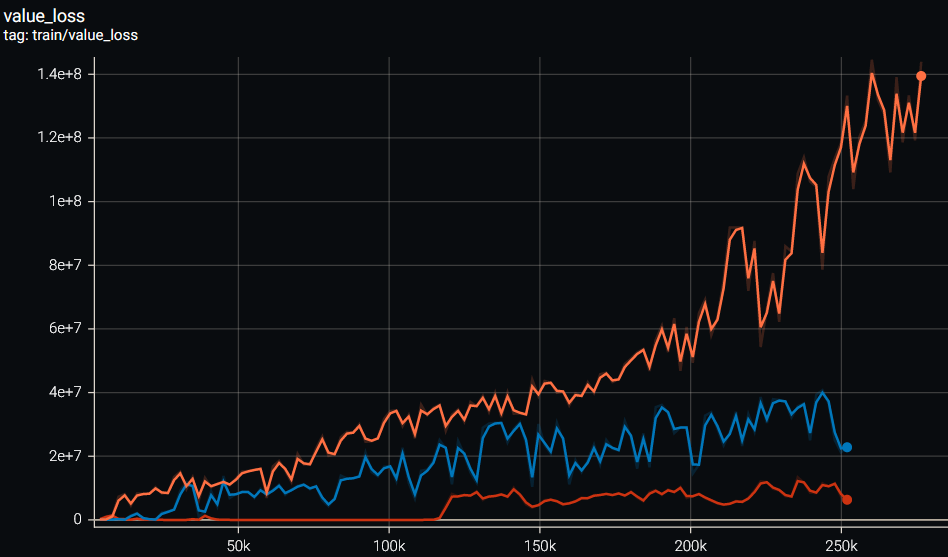
\includegraphics[width=10cm, height=7cm]{MyThesisImages/media/movement bad value_loss.PNG}}\\
  \hline
  STD &\raisebox{-0.5cm}{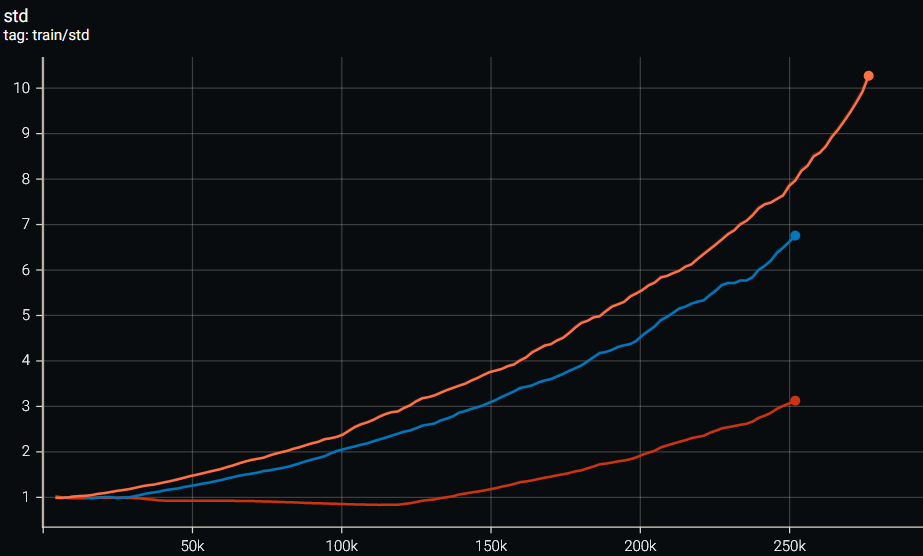
\includegraphics[width=10cm, height=7cm]{MyThesisImages/media/movement bad STD.PNG}}\\
  \hline
  Entropy Loss &\raisebox{-0.5cm}{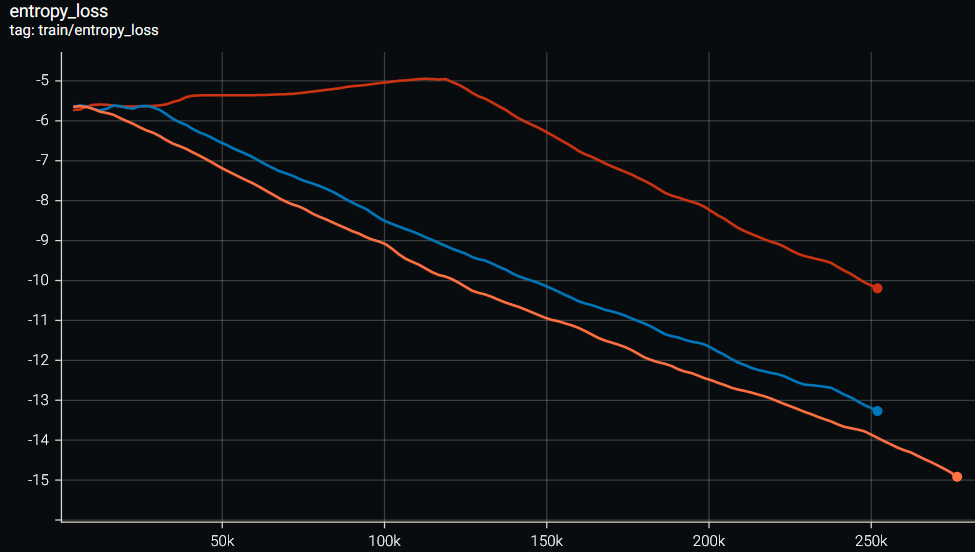
\includegraphics[width=10cm, height=7cm]{MyThesisImages/media/movement bad entropy_loss.PNG}}\\
  \hline
  Policy Gradient Loss &\raisebox{-0.5cm}{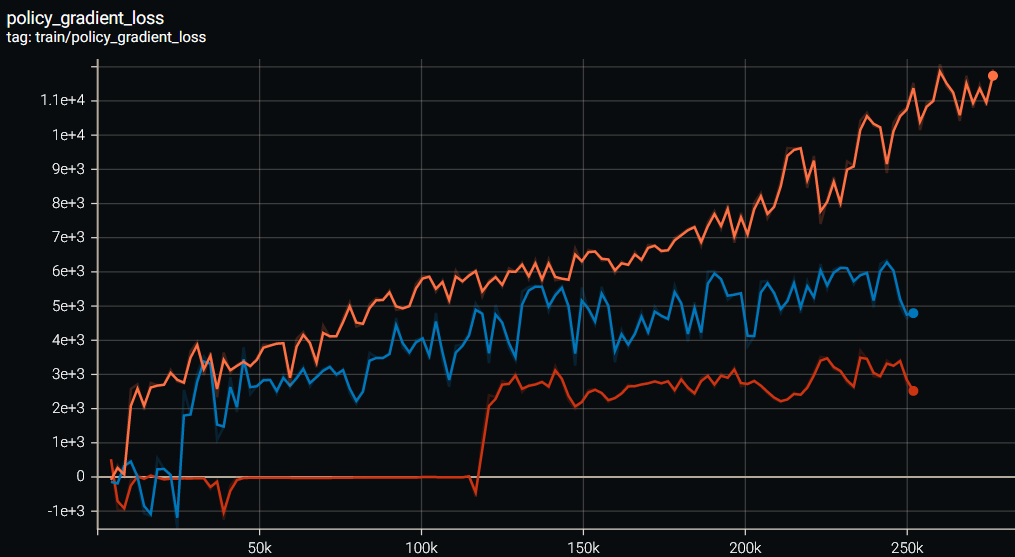
\includegraphics[width=10cm, height=7cm]{MyThesisImages/media/movement bad policy_gradient_loss.PNG}}\\
  \hline
  Approximate KL &\raisebox{-0.5cm}{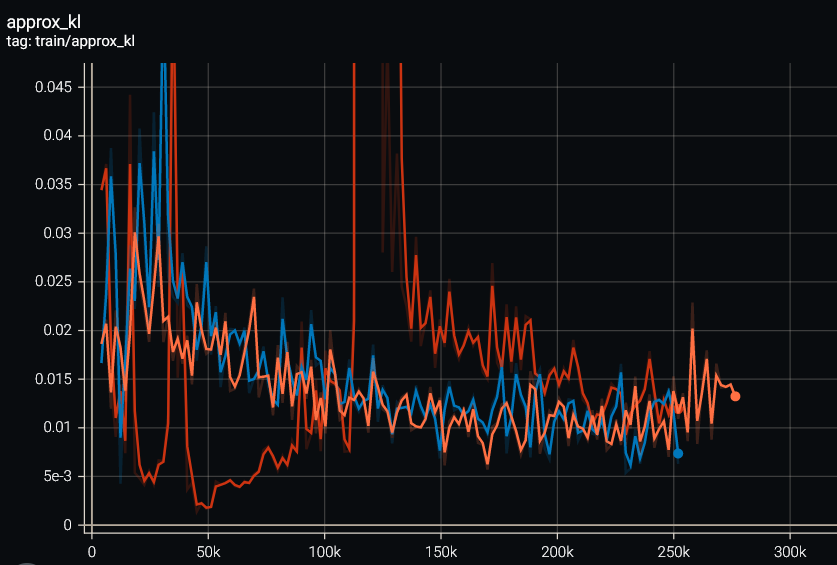
\includegraphics[width=10cm, height=7cm]{MyThesisImages/media/movement bad approximate_kl.PNG}}\\
  \hline
  Explained Variance &\raisebox{-0.5cm}{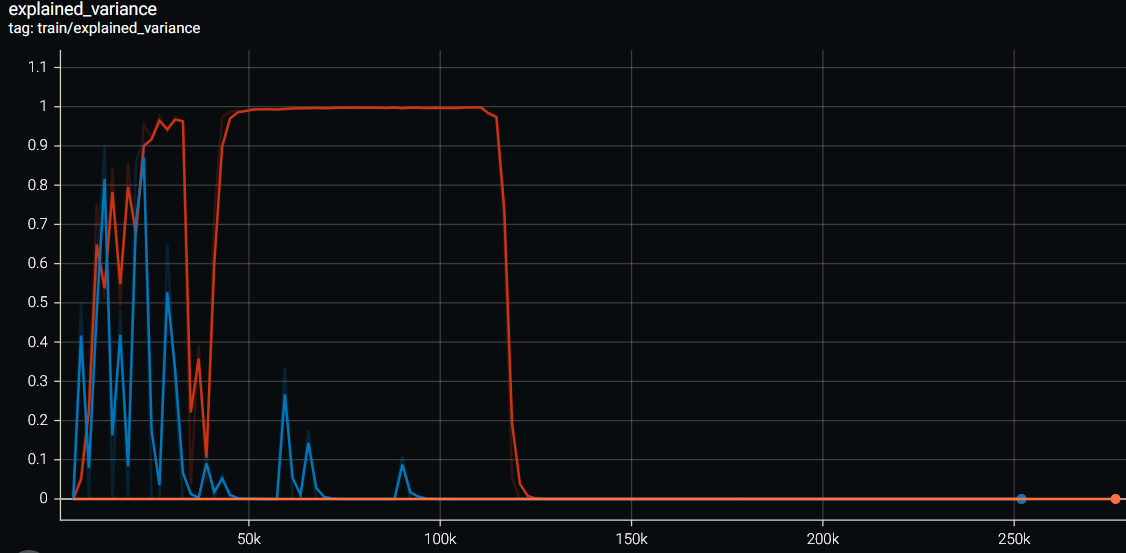
\includegraphics[width=10cm, height=7cm]{MyThesisImages/media/movement bad explained_variance.PNG}}\\
  \hline
  Clip Fraction &\raisebox{-0.5cm}{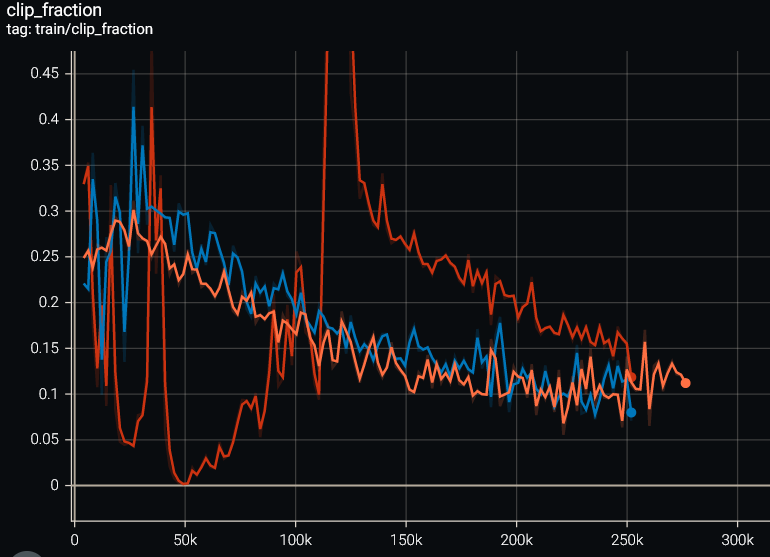
\includegraphics[width=10cm, height=7cm]{MyThesisImages/media/movement bad clip_fraction.PNG}}\\
  \hline

  \caption{Movement experiment 1 scalar curves. Three runs of the first experiment with different Observation spaces. Orange is a run with distance only, Blue is a run with distance + xy location, Dark Orange is a run with distance + xy location + camera rotation.}
\end{longtable} 

\begin{longtable}[H]
  {|m{5.5em}||m{23.5em}|}
  \hline
  Value Loss &\raisebox{-0.5cm}{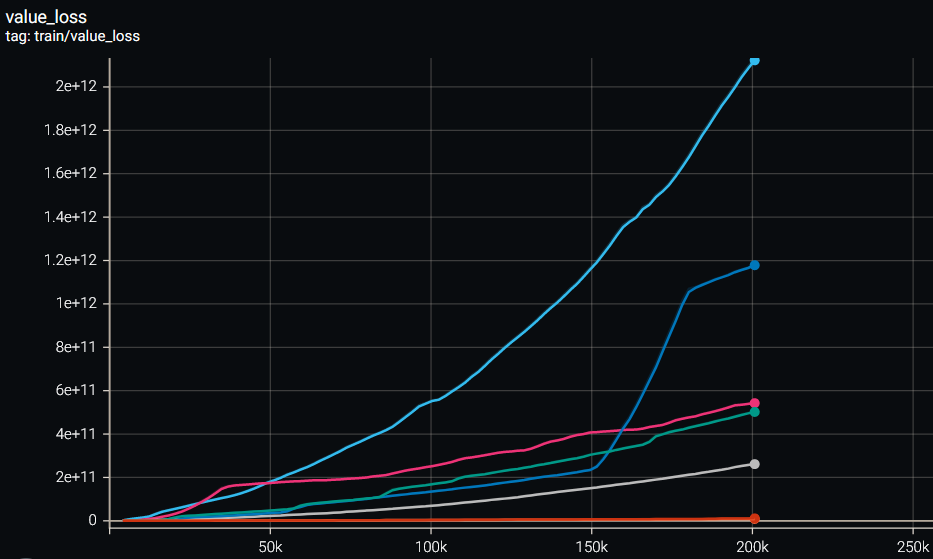
\includegraphics[width=10cm, height=7cm]{MyThesisImages/media/movement improved value_loss.PNG}}\\
  \hline
  STD &\raisebox{-0.5cm}{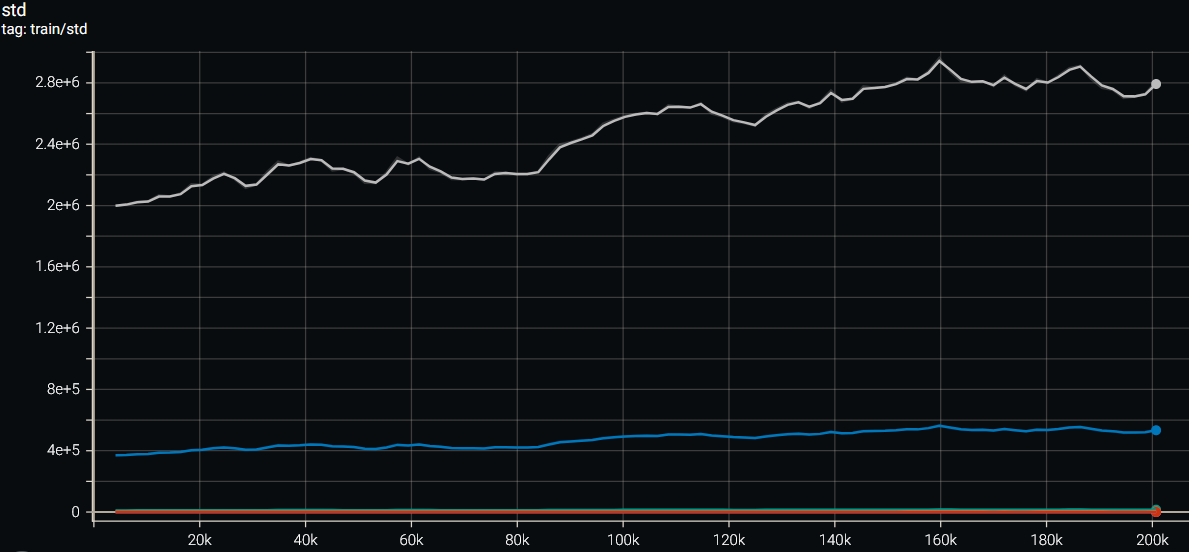
\includegraphics[width=10cm, height=7cm]{MyThesisImages/media/movement improved STD.PNG}}\\
  \hline
  Entropy Loss &\raisebox{-0.5cm}{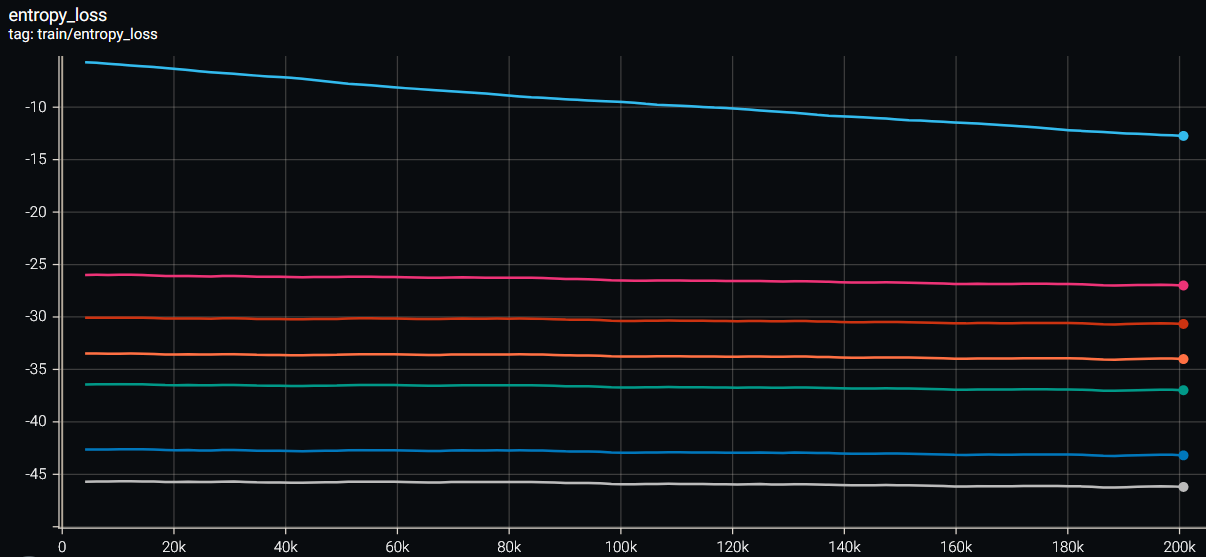
\includegraphics[width=10cm, height=7cm]{MyThesisImages/media/movement improved entropy_loss.PNG}}\\
  \hline
  Policy Gradient Loss &\raisebox{-0.5cm}{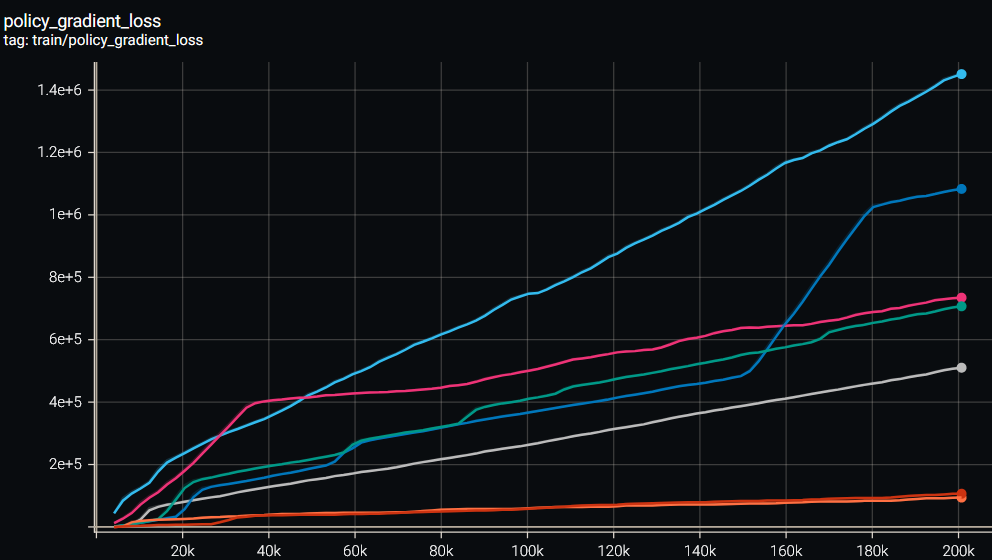
\includegraphics[width=10cm, height=7cm]{MyThesisImages/media/movement improved policy_gradient_loss.PNG}}\\
  \hline
  Approximate KL &\raisebox{-0.5cm}{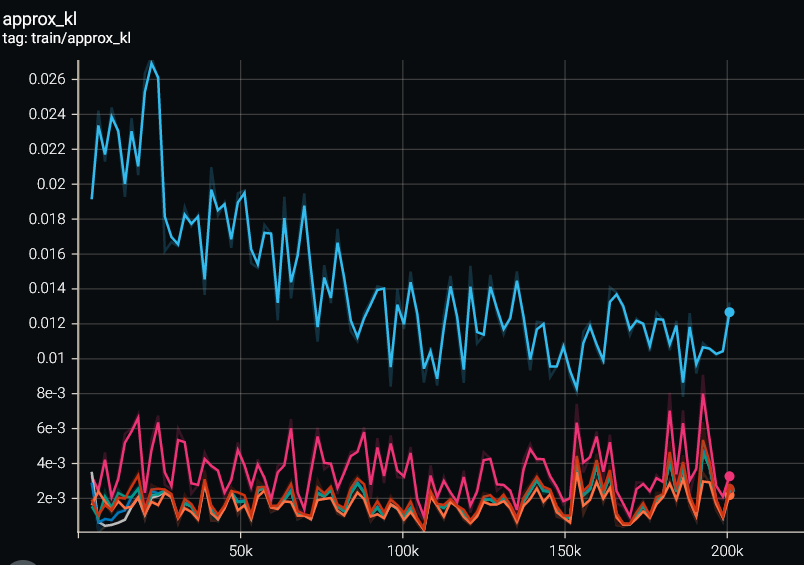
\includegraphics[width=10cm, height=7cm]{MyThesisImages/media/movement improved approximate_kl.PNG}}\\
  \hline
  Explained Variance &\raisebox{-0.5cm}{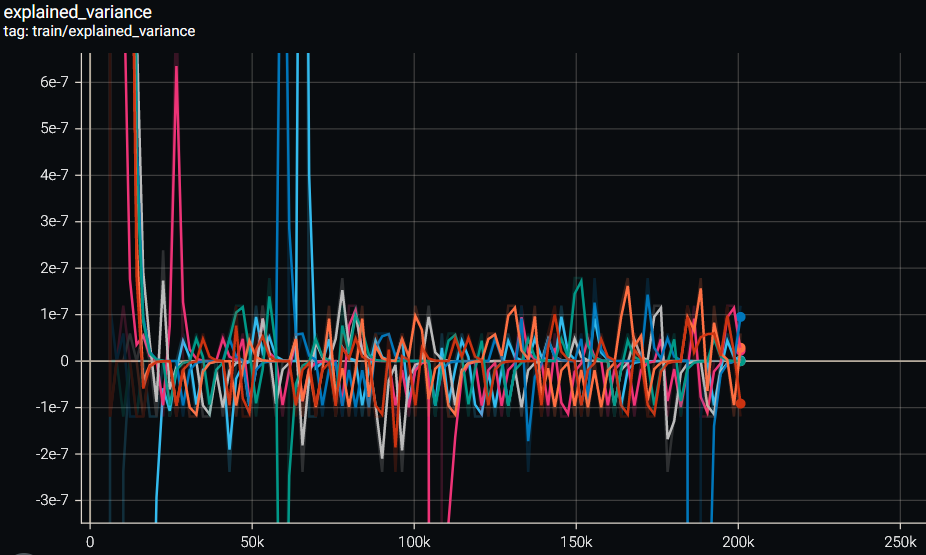
\includegraphics[width=10cm, height=7cm]{MyThesisImages/media/movement improved explained_variance.PNG}}\\
  \hline
  Clip Fraction &\raisebox{-0.5cm}{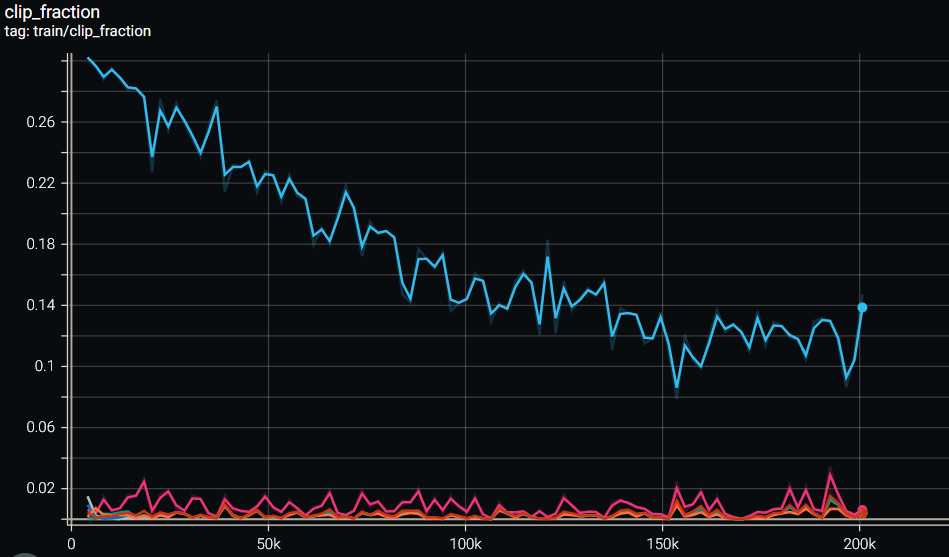
\includegraphics[width=10cm, height=7cm]{MyThesisImages/media/movement improved clip_fraction.PNG}}\\
  \hline

  \caption{Movement experiment 2 scalar curves. Light Blue is session 1, Pink is session 6, Dark Orange is session 11, Orange is session 16, Dark Green is session 21, Blue is session 31, White is session 36}
\end{longtable} 

\begin{longtable}[H]
  {|m{5.5em}||m{23.5em}|}
  \hline
  Value Loss &\raisebox{-0.5cm}{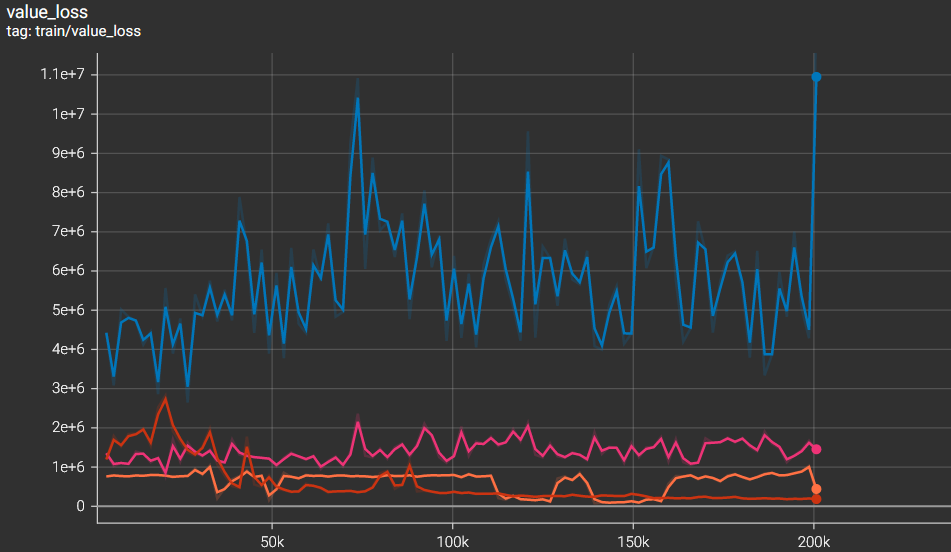
\includegraphics[width=10cm, height=7cm]{MyThesisImages/media/aiming no shooting value_loss.PNG}}\\
  \hline
  STD &\raisebox{-0.5cm}{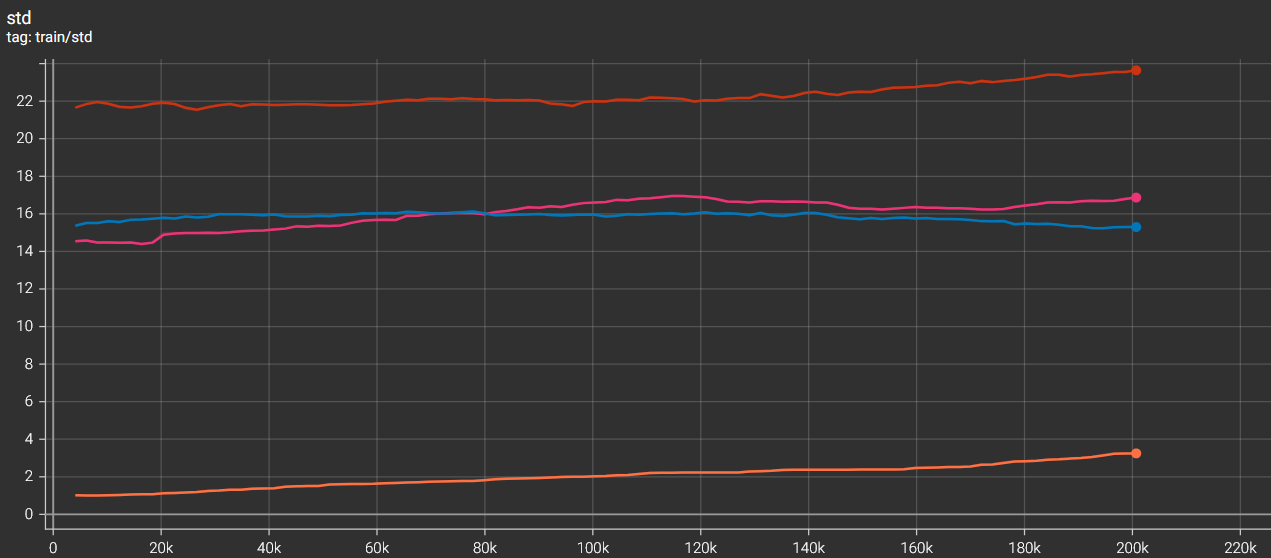
\includegraphics[width=10cm, height=7cm]{MyThesisImages/media/aiming no shooting std.PNG}}\\
  \hline
  Entropy Loss &\raisebox{-0.5cm}{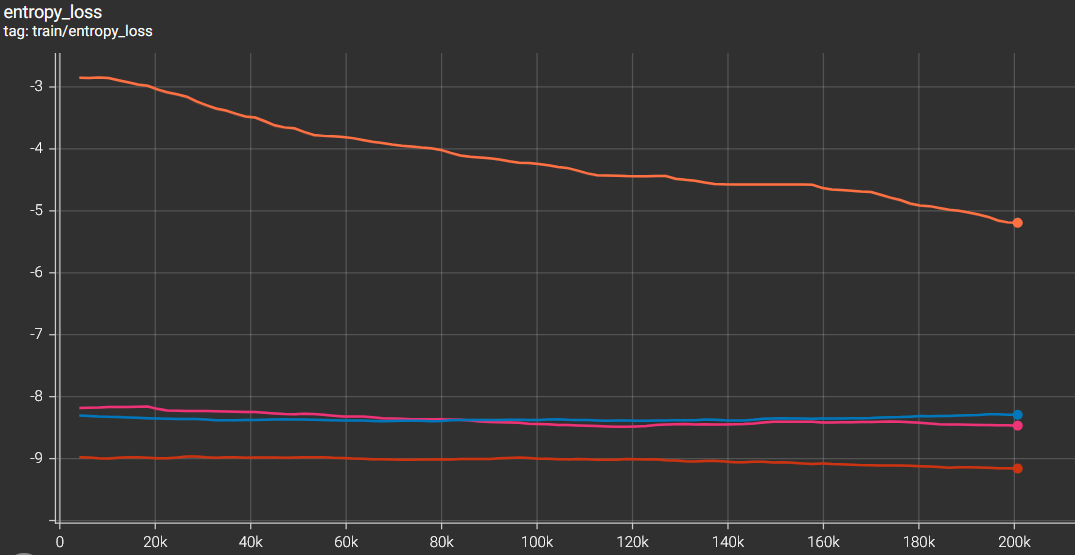
\includegraphics[width=10cm, height=7cm]{MyThesisImages/media/aiming no shooting entropy_loss.PNG}}\\
  \hline
  Policy Gradient Loss &\raisebox{-0.5cm}{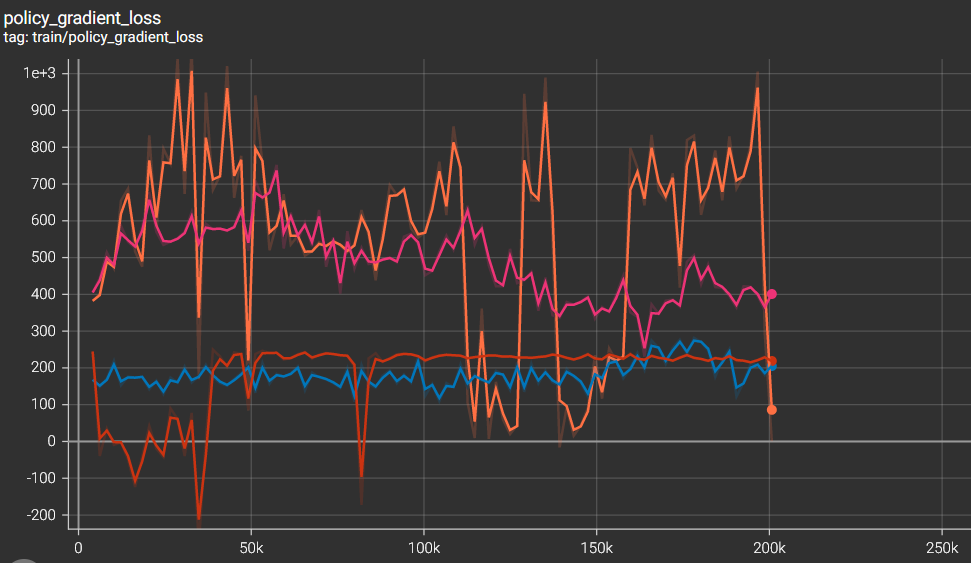
\includegraphics[width=10cm, height=7cm]{MyThesisImages/media/aiming no shooting policy_gradient_loss.PNG}}\\
  \hline
  Approximate KL &\raisebox{-0.5cm}{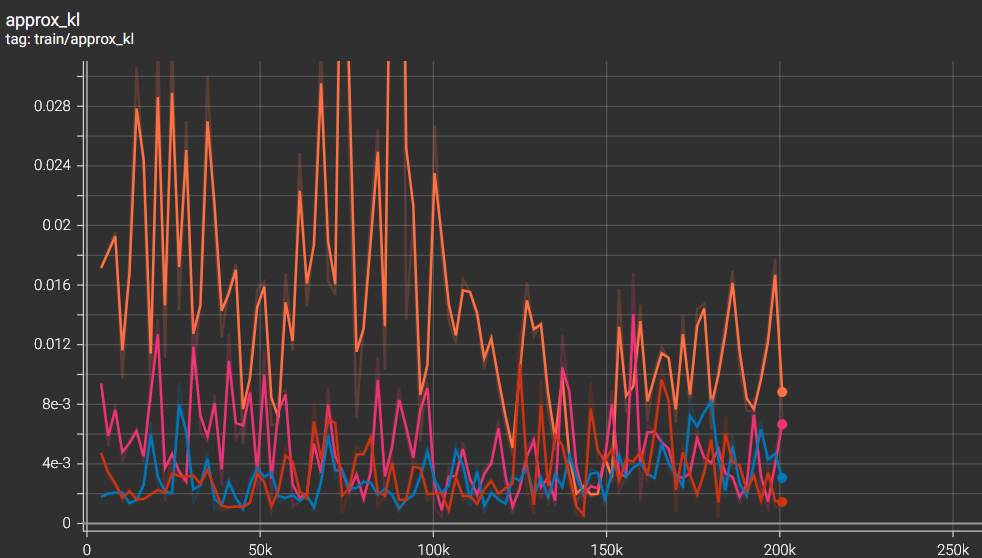
\includegraphics[width=10cm, height=7cm]{MyThesisImages/media/aiming no shooting approx_kl.PNG}}\\
  \hline
  Explained Variance &\raisebox{-0.5cm}{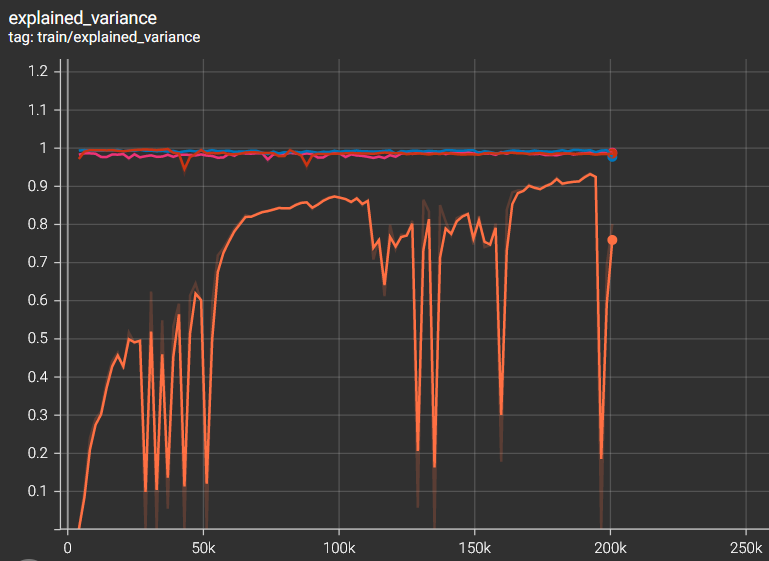
\includegraphics[width=10cm, height=7cm]{MyThesisImages/media/aiming no shooting explained_variance.PNG}}\\
  \hline
  Clip Fraction &\raisebox{-0.5cm}{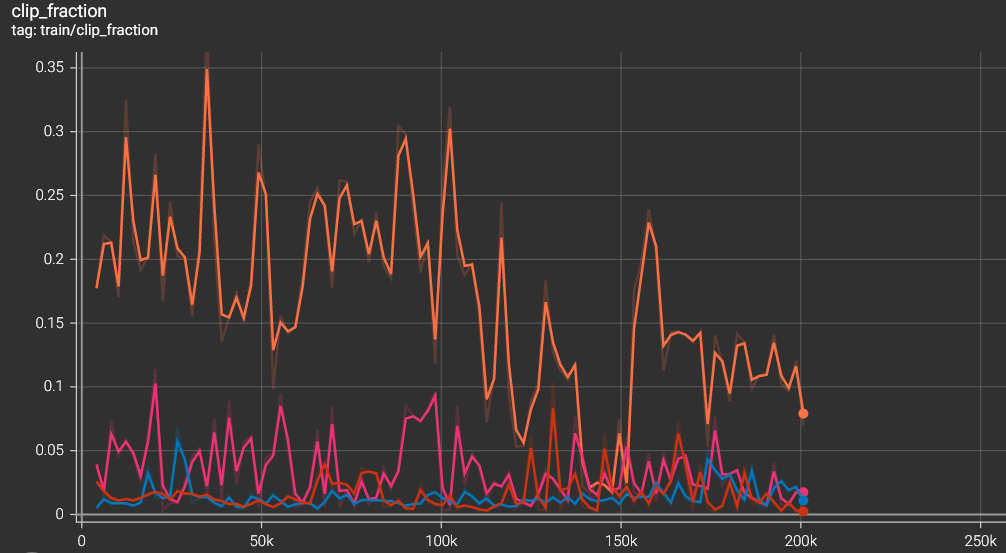
\includegraphics[width=10cm, height=7cm]{MyThesisImages/media/aiming no shooting clip_fraction.PNG}}\\
  \hline

  \caption{Aiming experiment 3 scalar curves. Orange is session 1, Pink is session 5, Dark Orange is session 10, Blue is session 16}
\end{longtable} 

\begin{longtable}[H]
  {|m{5.5em}||m{23.5em}|}
  \hline
  Value Loss &\raisebox{-0.5cm}{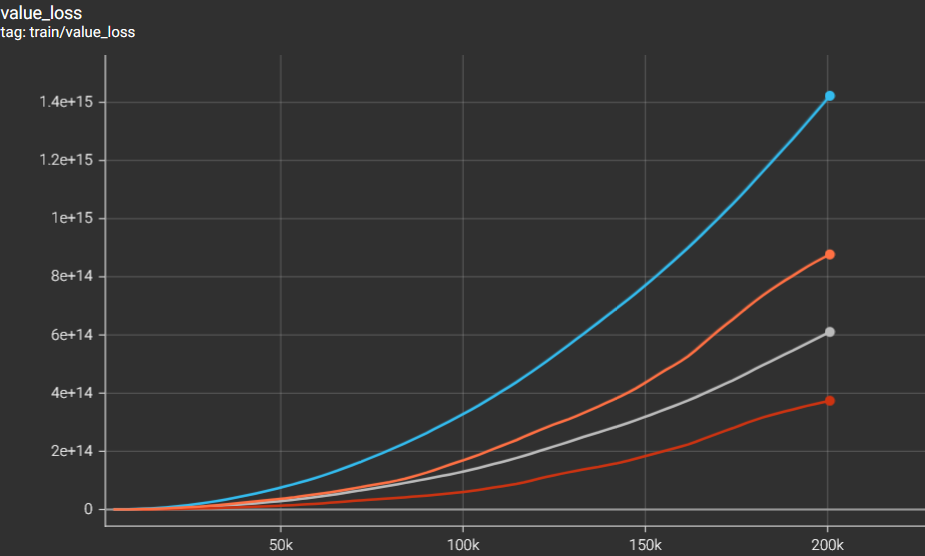
\includegraphics[width=10cm, height=7cm]{MyThesisImages/media/aiming shooting value_loss.PNG}}\\
  \hline
  STD &\raisebox{-0.5cm}{\includegraphics[width=10cm, height=7cm]{MyThesisImages/media/aiming shooting std.PNG}}\\
  \hline
  Entropy Loss &\raisebox{-0.5cm}{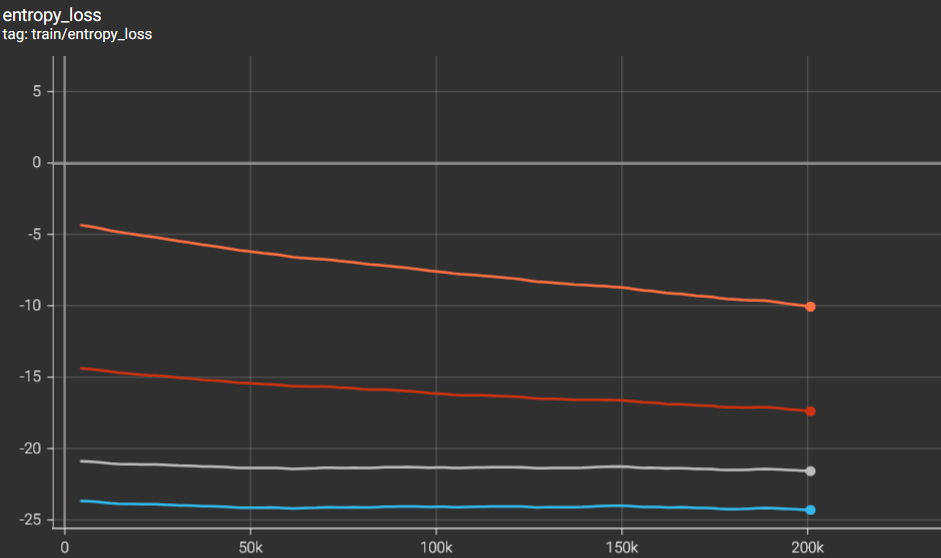
\includegraphics[width=10cm, height=7cm]{MyThesisImages/media/aiming shooting entropy_loss.PNG}}\\
  \hline
  Policy Gradient Loss &\raisebox{-0.5cm}{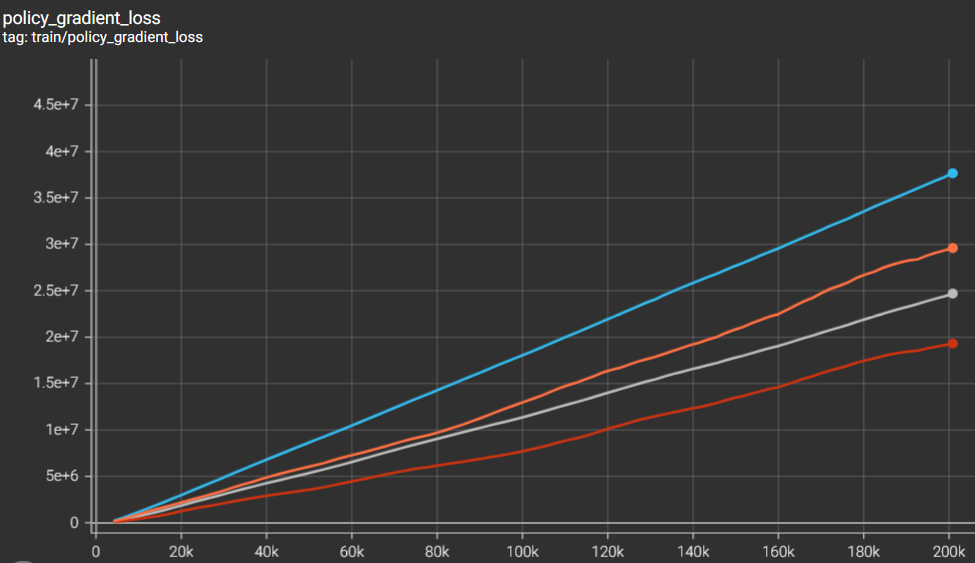
\includegraphics[width=10cm, height=7cm]{MyThesisImages/media/aiming shooting policy_gradient_loss.PNG}}\\
  \hline
  Approximate KL &\raisebox{-0.5cm}{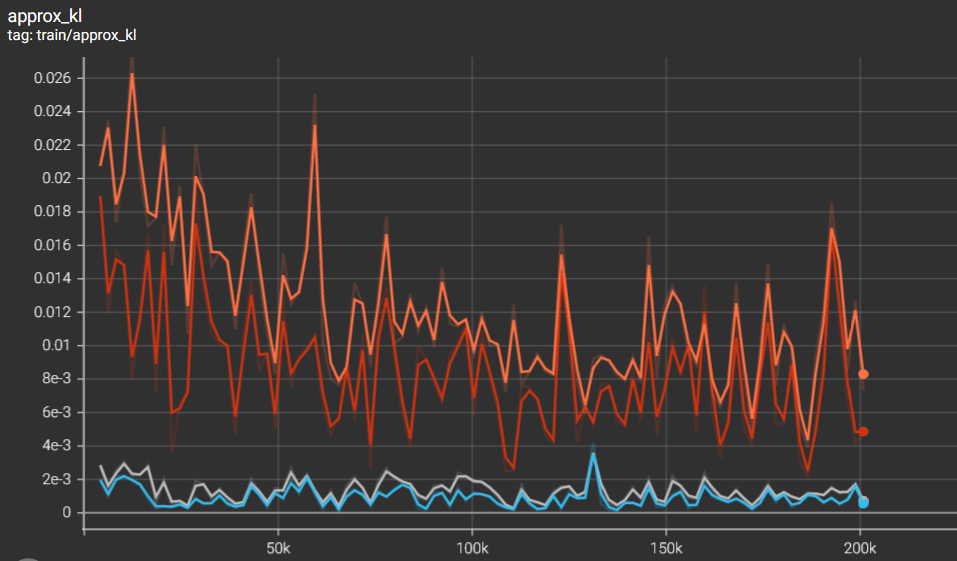
\includegraphics[width=10cm, height=7cm]{MyThesisImages/media/aiming shooting approximate_kl.PNG}}\\
  \hline
  Explained Variance &\raisebox{-0.5cm}{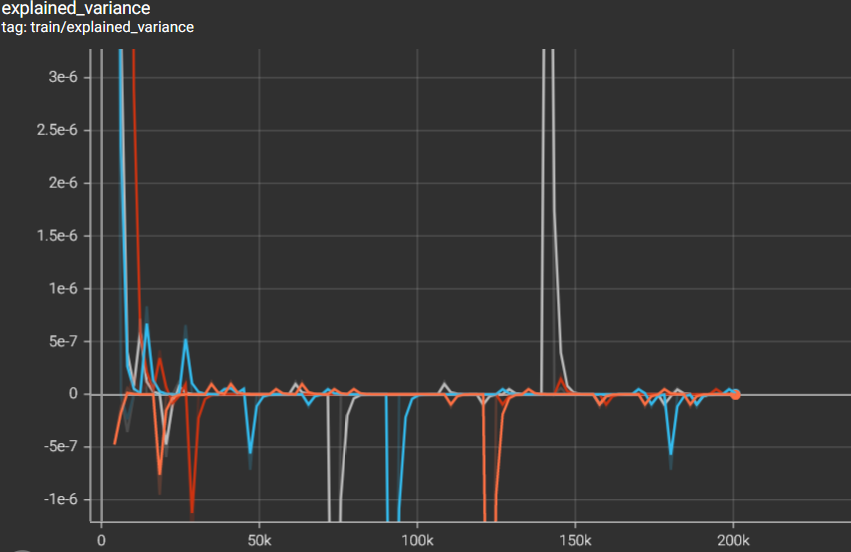
\includegraphics[width=10cm, height=7cm]{MyThesisImages/media/aiming shooting explained_variance.PNG}}\\
  \hline
  Clip Fraction &\raisebox{-0.5cm}{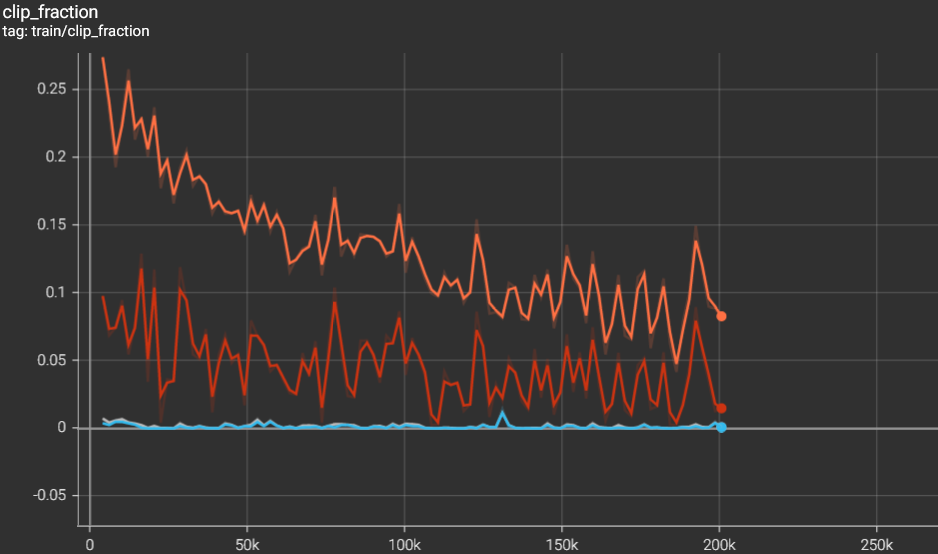
\includegraphics[width=10cm, height=7cm]{MyThesisImages/media/aiming shooting clip_fraction.PNG}}\\
  \hline

  \caption{Aiming+shooting experiment 4 scalar curves. Orange is session 1, Dark Orange is session 3, White is session 7, Blue is session 11}
\end{longtable} 

\section{(Sub-chapter 6.4) Adapting Unreal Engine Environment for Real-World Applications Simulation}

Training agents inside the unreal engine just like the demo game created for the thesis is only one of many possibilities focused on training game AI behavior. Most autonomous robots or other autonomous decision-making systems were mainly driven by complex algorithms which analyzed the sensor input data to perform predefined actions. With the rise of machine learning along with the significantly increased hardware performance, research has made a shift to training autonomous agents for commercial and industrial applications.
Bonsai\cite{bonsai_2020} was one of the first companies to focus on implementing RL to industrial applications and was acquired by Microsoft in 2018 that wanted to dive into creating "brains" for autonomous systems\cite{gurdeep_2018}.

A way of utilizing this combination of Game development and Deep
Reinforcement learning technology, is to use the capabilities of the
realistic simulation environment to recreate real-world scenarios and
train agents to deal with them, with a final goal of exporting the
trained AIs for use in real-world applications.

The designing process is not much different as we can get access to
every variable in real-world just like inside the simulation environment using specialized hardware.\\

\textbf{Most Common conversions to hardware:
}
\begin{itemize}
\item
  Get world location $\longleftrightarrow$ GPS
\item
  Line Trace Hit $\longleftrightarrow$  LiDAR Sensor
\item
  In game Camera $\longleftrightarrow$  Conventional Camera
\item
  Pixel Depth $\longleftrightarrow$  LiDAR Camera
\item
  Post Process Effect $\longleftrightarrow$  Infrared Camera
\end{itemize}

After carefully analyzing every possible real-world interaction and
recreating a detailed approximation of the environment, that the agent
will be eventually placed into, training inside unreal engine can be
conducted safely and with very low cost, avoiding hardware damage in
the initial phases when the agent will learn the environment.

There are three different options for utilizing this technology:

\begin{enumerate}
\def\labelenumi{\arabic{enumi}.}
\item
  Part of the training can be done by simulation and when it is decided
  the agent has reached a certain degree of the desired final behavior,
  it can be exported and continue to train using the real hardware.
\item
  Most of the training (85-95\%) can be done inside the simulation
  environment and then for the last 5-15\% the model can be finetuned in
  the real world.
\item
  All the training can be done inside the simulation environment and
  then export the final model for use in the real world.
\end{enumerate}

Applications vary from commercial, industrial, medical and military use.

\begin{itemize}
\item
  Robot control (commercial and industrial)
\item
  Vehicle driving (assistive or complete control)
\item
  Fire prevention and suppression
\item 
  Patient Vitals Monitoring
\item 
  Drug dosing
\item
  Remote terrain reconnaissance
\item
  Unmanned combat (Air and Land)
\end{itemize}

As this technology matures, applications utilizing autonomous AIs will
become more common, people will start getting comfortable being around
autonomous systems and having them assist or take over control in
certain scenarios, which will drive the market to invest in researching
this specialized field of computer science.

\pagebreak

\chapter{CHAPTER 7 CONCLUSIONS}

Video games earned a place among the largest entertainment industries,
even though there was a big gap between the scientific community and
game development industry in the past, it is gradually getting smaller
in recent years. Researchers have started to take video games seriously
and focus on implementing current technology and even developing new
one, for use in video games.

Video game development is a complex process combining artistic and
technical components in a sophisticated way to create a final product.
With the rise of deep learning and generative AI, capabilities have
increased significantly, revealing endless possibilities.

In this thesis some of the latest scientific literature was discussed
with a game development perspective, from behavioral artificial
intelligence building and improving upon traditional technics, to the
latest generative AI methods using GANs, VAEs and Diffusion based models
for content generation. Only a few scientists focus on videogame
specific research, but the promising results will surely drive the video
game industry to invest more resources for enticing further specialized
research.

A wide variety of AI based tools can be found online and developers can
have access to them in order to greatly enhance their arsenal with
minimal or no cost, compared to the traditional method of creating
everything by hand. Although the technology has not progressed enough to
meet the AAA game standards, a very good result can be achieved.

The video game industry is continuously changing and evolving in order
to meet and even exceed consumer expectations, it is inevitable that
artificial intelligence will definitely make its way inside the workflow
of game development process. Not as much as replacing the human aspect
but optimizing productivity, driving down costs and creating the
environment for faster turnover times. Big studios will be the last to
integrate such systems at least at the production level, as the
technology has not matured enough to meet the highest standards
demanded.

The last chapter focused on how a game engine can be leveraged as a
simulation environment to train Deep RL agents and how to design and
implement them inside Unreal Engine. It is a very intuitive process
especially with the use of the Blueprint visual scripting environment,
but it is a very computationally demanding task that will require
incredible amounts of training time. The more complex the desired
behavior the more difficult it will be to train a single agent, the use
of methods such as multi-agent training may be necessary for reducing
training times significantly and creating a realistic timeframe in which
a model can be trained and transferred for use in a real-world
application but with a huge increase of computational cost.

In the near future, AI technology will penetrate many industries
including the video game development scene. The use of AI will become
commonplace during development as well as in postproduction applications
due to its many advantages it can bring to the table but will also
leverage the simulation capabilities of the video game world to continue
evolving itself.

\pagebreak

\printbibliography[heading=bibintoc,title={BIBLIOGRAPHY}]

\end{document}